 % arara: clean: { files: [thesis.aux, thesis.bbl, thesis.blg, thesis.dvi, thesis.fdb_latexmk, thesis.fls, thesis.idx, thesis.ilg, thesis.ind, thesis.lof, thesis.log, thesis.lot, thesis.nlo, thesis.nls, thesis.out, thesis.pdf, thesis.ps, thesis.toc]}
% arara: latex:  { shell: yes }
% arara: bibtex
% arara: nomencl
% arara: latex
% arara: makeindex
% arara: latex:  { shell: yes }
% arara: dvips
% arara: ps2pdf

% ******************************* PhD Thesis Template **************************
% Please have a look at the README.md file for info on how to use the template

\documentclass[a4paper,12pt,times,numbered,print,index,draftmode,chapter]{Classes/PhDThesisPSnPDF}
% add "chapter" to only print out select chapters (defined below)

% ******************************************************************************
% ******************************* Class Options ********************************
% *********************** See README for more details **************************
% ******************************************************************************

% `a4paper'(The University of Cambridge PhD thesis guidelines recommends a page
% size a4 - default option) or `a5paper': A5 Paper size is also allowed as per
% the Cambridge University Engineering Deparment guidelines for PhD thesis
%
% `11pt' or `12pt'(default): Font Size 10pt is NOT recommended by the University
% guidelines
%
% `oneside' or `twoside'(default): Printing double side (twoside) or single
% side.
%
% `print': Use `print' for print version with appropriate margins and page
% layout. Leaving the options field blank will activate Online version.
%
% `index': For index at the end of the thesis
%
% `draft': For draft mode without loading any images (same as draft in book)
%
% `draftmode': Special draft mode with line numbers, images, and water mark with
% timestamp and custom text. Position of the text can also be modified.
%
% `abstract': To generate only the title page and abstract page with
% dissertation title and name, to submit to the Student Registry
%
% `chapter`: This option enables only the specified chapter and it's references
%  Useful for review and corrections.
%
% ************************* Custom Page Margins ********************************
%
% `custommargin`: Use `custommargin' in options to activate custom page margins,
% which can be defined in the preamble.tex. Custom margin will override
% print/online margin setup.
%
% *********************** Choosing the Fonts in Class Options ******************
%
% `times' : Times font with math support. (The Cambridge University guidelines
% recommend using times)
%
% `fourier': Utopia Font with Fourier Math font (Font has to be installed)
%            It's a free font.
%
% `customfont': Use `customfont' option in the document class and load the
% package in the preamble.tex
%
% default or leave empty: `Latin Modern' font will be loaded.
%
% ********************** Choosing the Bibliography style ***********************
%
% `authoryear': For author-year citation eg., Krishna (2013)
%
% `numbered': (Default Option) For numbered and sorted citation e.g., [1,5,2]
%
% `custombib': Define your own bibliography style in the `preamble.tex' file.
%              `\RequirePackage[square, sort, numbers, authoryear]{natbib}'.
%              This can be also used to load biblatex instead of natbib
%              (See Preamble)
%
% **************************** Choosing the Page Style *************************
%
% `default (leave empty)': For Page Numbers in Header (Left Even, Right Odd) and
% Chapter Name in Header (Right Even) and Section Name (Left Odd). Blank Footer.
%
% `PageStyleI': Chapter Name next & Page Number on Even Side (Left Even).
% Section Name & Page Number in Header on Odd Side (Right Odd). Footer is empty.
%
% `PageStyleII': Chapter Name on Even Side (Left Even) in Header. Section Number
% and Section Name in Header on Odd Side (Right Odd). Page numbering in footer


\newcommand{\nj}{\ensuremath{n_{\text{jet}}}\xspace}
\newcommand{\njlow}{\ensuremath{2 \leq \njet \leq 3}\xspace}
\newcommand{\njhigh}{\ensuremath{\njet \geq 4}\xspace}
\newcommand{\nb}{\ensuremath{n_{\text{b}}}\xspace}
\newcommand{\alphat}{\ensuremath{\alpha_{\text{T}}}\xspace}
\newcommand{\htalphat}{\texttt{HT\_AlphaT}\xspace}
\newcommand{\photon}{\texttt{Photon}\xspace}
\newcommand{\mt}{\ensuremath{M_{\textrm T}}\xspace}
\newcommand{\gj}{\ensuremath{\gamma} + jets\xspace}
\newcommand{\mj}{\ensuremath{\mu} + jets\xspace}
\newcommand{\mmj}{\ensuremath{\mu\mu} + jets\xspace}
\newcommand{\npre}{\ensuremath{N_{\textrm{pred}}}\xspace}
\newcommand{\nobs}{\ensuremath{N_{\textrm{obs}}}\xspace}
\newcommand{\njets}{\ensuremath{N_{\textrm{jet}}}\xspace}
\newcommand{\sq}{\ensuremath{\tilde{\rm q}}\xspace}
\newcommand{\st}{\ensuremath{\tilde{\rm t}}\xspace}
\newcommand{\gl}{\ensuremath{\tilde{\rm g}}\xspace}
\newcommand{\ewk}{\ensuremath{\mathrm{EWK}}\xspace}
\newcommand{\qcd}{\ensuremath{\mathrm{QCD}}\xspace}
\newcommand{\zInv}[1]{\ensuremath{Z_{\rm inv}^{#1}}\xspace}
\newcommand{\Pt}{\ensuremath{{p_{\text T}}}\xspace}
\newcommand{\dphi}{\ensuremath{\Delta \phi}}
\newcommand{\Et}{\ensuremath{{E_{\text T}}}\xs}
\newcommand{\ttj}{\ensuremath{\rm{t}\bar{\rm{t}} + jets}\xspace}
\newcommand{\wj}{\ensuremath{\rm W + jets}\xspace}
\newcommand{\zj}{\ensuremath{\rm Z + jets}\xspace}
\newcommand{\fb}{\ensuremath{fb^{-1}}}
\newcommand{\HT}{\ensuremath{H_T}\xspace}

% % these might not work...!
\def\eslash{{\hbox{$E$\kern-0.6em\lower-.05ex\hbox{/}\kern0.10em}}}
\def\vecmet{\mbox{$\vec{\eslash}_T$}} %missing ET vector
\def\vecet{\mbox{$\vec{E}_\text{T}$}} % ET vector
\def\MET{\mbox{$\eslash_\text{T}$}\xspace}
\def\met{\mbox{$\eslash_\text{T}$}\xspace}
% \def\hslash{{\hbox{$H$\kern-0.8em\lower-.05ex\hbox{/}\kern0.10em}}}
\def\MHT{\mbox{$\hslash_\text{T}$}\xspace}
% \def\mht{\mbox{$\hslash_\text{T}$}\xspace}
% \def\mhtmet{\mbox{$\hslash_\text{T} / \eslash_\text{T}$}\xspace}
% \def\bdphi{\mbox{$\Delta\phi^{*}$}\xspace}

% ********************************** Preamble **********************************
% Preamble: Contains packages and user-defined commands and settings
% ******************************************************************************
% ****************************** Custom Margin *********************************

% Add `custommargin' in the document class options to use this section
% Set {innerside margin / outerside margin / topmargin / bottom margin}  and
% other page dimensions
\ifsetCustomMargin
  \RequirePackage[left=37mm,right=30mm,top=35mm,bottom=30mm]{geometry}
  \setFancyHdr % To apply fancy header after geometry package is loaded
\fi

% *****************************************************************************
% ******************* Fonts (like different typewriter fonts etc.)*************

% Add `customfont' in the document class option to use this section

\ifsetCustomFont
  % Set your custom font here and use `customfont' in options. Leave empty to
  % load computer modern font (default LaTeX font).
  \RequirePackage{helvet}
\fi

% *****************************************************************************
% **************************** Custom Packages ********************************

% ************************* Algorithms and Pseudocode **************************

%\usepackage{algpseudocode}


% ********************Captions and Hyperreferencing / URL **********************

% Captions: This makes captions of figures use a boldfaced small font.
%\RequirePackage[small,bf]{caption}

\RequirePackage[labelsep=space,tableposition=top]{caption}
\renewcommand{\figurename}{Fig.} %to support older versions of captions.sty


% *************************** Graphics and figures *****************************

%\usepackage{rotating}
%\usepackage{wrapfig}

% Uncomment the following two lines to force Latex to place the figure.
% Use [H] when including graphics. Note 'H' instead of 'h'
%\usepackage{float}
%\restylefloat{figure}

% Subcaption package is also available in the sty folder you can use that by
% uncommenting the following line
% This is for people stuck with older versions of texlive
%\usepackage{sty/caption/subcaption}
\usepackage{subcaption}
\usepackage{xspace}

% ********************************** Tables ************************************
\usepackage{booktabs} % For professional looking tables
\usepackage{multirow}

%\usepackage{multicol}
%\usepackage{longtable}
%\usepackage{tabularx}


% ***************************** Math and SI Units ******************************

\usepackage{amsfonts}
\usepackage{amsmath}
\usepackage{amssymb}
\usepackage{siunitx} % use this package module for SI units
\usepackage[makeroom]{cancel}


% ******************************* Line Spacing *********************************

% Choose linespacing as appropriate. Default is one-half line spacing as per the
% University guidelines

% \doublespacing
\onehalfspacing
% \singlespacing


% ************************ Formatting / Footnote *******************************

%\usepackage[perpage]{footmisc} %Range of footnote options


% *****************************************************************************
% *************************** Bibliography  and References ********************

%\usepackage{cleveref} %Referencing without need to explicitly state fig /table

% Add `custombib' in the document class option to use this section
\ifuseCustomBib
   \RequirePackage[square, sort, numbers, authoryear]{natbib} % CustomBib

% If you would like to use biblatex for your reference management, as opposed to the default `natbibpackage` pass the option `custombib` in the document class. Comment out the previous line to make sure you don't load the natbib package. Uncomment the following lines and specify the location of references.bib file

%\RequirePackage[backend=biber, style=numeric-comp, citestyle=numeric, sorting=nty, natbib=true]{biblatex}
%\bibliography{References/references} %Location of references.bib only for biblatex

\fi

% changes the default name `Bibliography` -> `References'
\renewcommand{\bibname}{References}


% *****************************************************************************
% *************** Changing the Visual Style of Chapter Headings ***************
% This section on visual style is from https://github.com/cambridge/thesis

% Uncomment the section below. Requires titlesec package.

%\RequirePackage{titlesec}
%\newcommand{\PreContentTitleFormat}{\titleformat{\chapter}[display]{\scshape\Large}
%{\Large\filleft{\chaptertitlename} \Huge\thechapter}
%{1ex}{}
%[\vspace{1ex}\titlerule]}
%\newcommand{\ContentTitleFormat}{\titleformat{\chapter}[display]{\scshape\huge}
%{\Large\filleft{\chaptertitlename} \Huge\thechapter}{1ex}
%{\titlerule\vspace{1ex}\filright}
%[\vspace{1ex}\titlerule]}
%\newcommand{\PostContentTitleFormat}{\PreContentTitleFormat}
%\PreContentTitleFormat


% ******************************************************************************
% ************************* User Defined Commands ******************************
% ******************************************************************************

% *********** To change the name of Table of Contents / LOF and LOT ************

%\renewcommand{\contentsname}{My Table of Contents}
%\renewcommand{\listfigurename}{My List of Figures}
%\renewcommand{\listtablename}{My List of Tables}


% ********************** TOC depth and numbering depth *************************

\setcounter{secnumdepth}{2}
\setcounter{tocdepth}{2}


% ******************************* Nomenclature *********************************

% To change the name of the Nomenclature section, uncomment the following line

%\renewcommand{\nomname}{Symbols}


% ********************************* Appendix ***********************************

% The default value of both \appendixtocname and \appendixpagename is `Appendices'. These names can all be changed via:

%\renewcommand{\appendixtocname}{List of appendices}
%\renewcommand{\appendixname}{Appndx}

% ******************************** Draft Mode **********************************

% Uncomment to disable figures in `draftmode'
\setkeys{Gin}{draft=false}  % set draft to false to enable figures in `draft'

% These options are active only during the draft mode
% Default text is "Draft"
\SetDraftText{DRAFT}

% Default Watermark location is top. Location (top/bottom)
\SetDraftWMPosition{top}

% Draft Version - default is v1.0
%\SetDraftVersion{v1.1}

% Draft Text grayscale value (should be between 0-black and 1-white)
% Default value is 0.75
%\SetDraftGrayScale{0.8}


% ************************ Thesis Information & Meta-data **********************
% Thesis title and author information, refernce file for biblatex
% ************************ Thesis Information & Meta-data **********************
%% The title of the thesis
% \title{Searching for Supersymmetry in the all-hadronic channel with the \alphat 
% kinematic variable at CMS}
\title{My thesis it's really great might find SUSY.}
%\texorpdfstring is used for PDF metadata. Usage:
%\texorpdfstring{LaTeX_Version}{PDF Version (non-latex)} eg.,
%\texorpdfstring{$sigma$}{sigma}

%% Subtitle (Optional)
% \subtitle{Using the CUED template}

%% The full name of the author
\author{Chris Lucas}

%% Department (eg. Department of Engineering, Maths, Physics)
\dept{School of Physics}

%% University and Crest
\university{University of Bristol}
\crest{
\includegraphics[width=0.25\textwidth]{uni_crest.png}}

%% You can redefine the submission text:
% Default as per the University guidelines: This dissertation is submitted for
% the degree of Doctor of Philosophy
%\renewcommand{\submissiontext}{change the default text here if needed}

%% Full title of the Degree
\degree{Doctor of Philosophy}

%% College affiliation (optional)
% \college{King's College}

%% Submission date
% Default is set as {\monthname[\the\month]\space\the\year}
%\degreedate{2014} 

%% Meta information
\subject{LaTeX} \keywords{{LaTeX} {PhD Thesis} {Physics} {University of Bristol}}


% ***************************** Abstract Separate ******************************
% To printout only the titlepage and the abstract with the PhD title and the
% author name for submission to the Student Registry, use the `abstract' option in
% the document class.

\ifdefineAbstract
 \pagestyle{empty}
 \includeonly{Declaration/declaration, Abstract/abstract}
\fi

% ***************************** Chapter Mode ***********************************
% The chapter mode allows user to only print particular chapters with references
% Title, Contents, Frontmatter are disabled by default
% Useful option to review a particular chapter or to send it to supervisior.
% To use choose `chapter' option in the document class

\ifdefineChapter
 \includeonly{Chapter4/chapter4}
\fi

% ******************************** Front Matter ********************************
\begin{document}

\frontmatter

\begin{titlepage}

\maketitle

\end{titlepage}

% ******************************* Thesis Dedidcation ********************************

\begin{dedication} 

I would like to dedicate this thesis to my loving parents and Michelle Obama \ldots

\end{dedication}


% ******************************* Thesis Declaration ***************************

\begin{declaration}

I hereby declare that except where specific reference is made to the work of 
others, the contents of this dissertation are original and have not been 
submitted in whole or in part for consideration for any other degree or 
qualification in this, or any other university. This dissertation is my own 
work and contains nothing which is the outcome of work done in collaboration 
with others, except as specified in the text and Acknowledgements. This 
dissertation contains fewer than 65,000 words including appendices, 
bibliography, footnotes, tables and equations and has fewer than 150 figures.

% Author and date will be inserted automatically from thesis.tex \author \degreedate

\end{declaration}


% ************************** Thesis Acknowledgements **************************

\begin{acknowledgements}      


And I would like to acknowledge ...


\end{acknowledgements}

% ************************** Thesis Abstract *****************************
% Use `abstract' as an option in the document class to print only the titlepage and the abstract.
\begin{abstract}
A search for Supersymmetry in the jets and missing energy final state is
described using the CMS detector at the LHC, and the full 18.5~\fb 
`Parked' dataset
of $\sqrt{s} = 8$~\tev proton-proton collisions. This dataset was collected
using experimental, low-threshold triggers to increase sensitivity to softly
decaying new physics signatures. The search makes use of the
kinematic variable, \alphat, to reduce contributions from QCD multijet
processes by many orders of magnitude, down to a negligible level. Remaining
background sources originate from electroweak decays of heavy bosons and top
quarks, and are
estimated using a data-driven technique employing dedicated control regions. To
maintain sensitivity to a broad range of potential
manifestations
of Supersymmetry, the analysis categorises events in dimensions of the scalar
sum of hadronic energy, the number of jets and the number of jets originating
from b-quarks.
While this analysis aims to remain inclusive to many hadronically decaying SUSY
signatures, the work in this thesis exploits the low energy thresholds of the
`Parked' triggers and therefore considers models with compressed mass spectra.
As no statistically significant excess is observed, results are
interpreted within the context of decays of stop
particles relevant in the compressed spectra region. Stop decays to charm
quarks and via four-body decays to fermions are considered, both with the weakly
interacting Lightest SUSY Particle in the final state.
Limits are placed on $m_{\sTop}$ up to 275 GeV for the charm decay
and 250 GeV for the four-body decay. Natural units ($\hbar = c = 1$) are used
throughout this work.
\end{abstract}



% *********************** Adding TOC and List of Figures ***********************

\tableofcontents

\listoffigures

\listoftables

% \printnomenclature[space] space can be set as 2.5cm between symbol and
% description
\printnomencl

% ******************************** Main Matter *********************************
\mainmatter

%*******************************************************************************
%*********************************** First Chapter *****************************
%*******************************************************************************

\chapter{Introduction}  %Title of the First Chapter

\ifpdf
    \graphicspath{{Chapter1/Figs/Raster/}{Chapter1/Figs/PDF/}{Chapter1/Figs/}}
\else
    \graphicspath{{Chapter1/Figs/Vector/}{Chapter1/Figs/}}
\fi


%********************************** % First Section  *************************************
%Section - 1.1 
\label{sec:introduction_intro}

Our instinctive method of understanding is reductive - the idea of an
inventor attempting to make sense of the things around them, is
that of toasters, clocks radios, or even gearboxes broken down into
their smallest constituent parts to better understand what they're made of and,
ultimately, what's happening inside of them. This simple idea translates
perfectly to explain the work Particle Physicists have been undertaking with
not simple everyday household objects, but the Universe.

Since the beginnings of the field, physicists have questioned
what is
around us, and what it's made of. From the early research of scientists such as
Ernest Rutherford and Niels Bohr, the basic building
blocks of the universe have been searched for. For Particle Physicists, this is
the ultimate goal - a complete understanding of the nature of the Universe
at it's most
fundamental level. If a description can be written of the smallest
building blocks of
nature and how they interact, then ultimately we can understand
the Universe from the ground up.

Currently, our best attempt comes from the intersection of two very different
fields: Quantum Mechanics, the study of microscopic objects, and Relativity, the
study of very fast objects. The combination of these
two contrasting worlds gave birth to the field of Relativistic
Quantum Mechanics, and ultimately, the Standard Model.

First proposed in the 1960s, the Standard Model attempts to describe the
properties of the fundamental constituents of matter, and outline their
interactions through three of the four fundamental forces of nature, as
described in chapter~\ref{ch:theory}. Through
it's accurate description and predictions of not only particles such as
the electrons, quarks and gluons of which atoms are composed,
as well as fundamental constants of nature such as the fine structure constant
$\alpha$, the
Standard Model has exceptionally proven itself to be a triumph of
modern physics.

Despite it's continued accuracy in the face of substantial scrutiny, however,
the Standard Model fails to account for significant observations, for example
the absent description of gravity and the `other' 96\% of particles in the
Universe - the so-called `Dark Universe'. Similarly the Standard Model fails to
unify the forces at some higher mass scale, or accurately predict the mass of
the newly
discovered Higgs boson. As such, given how successfully it describes what it
can, the SM is widely considered
as a smaller component of some greater, all-encompassing theory.
This belief has led many to use this distinct theory as a building
block, on which extensions can be introduced to create Beyond the Standard Model
(BSM) theories - the goal being to fix the gaps in knowledge left by the SM.

Of the plethora of BSM theories, one particularly well motivated extension is
Supersymmetry (SUSY). The so-called `Supersymmetric' extension to the Standard
Model introduces supersymmetryic particles (or `sparticles') differing from
their SM partners by half a unit of spin - described in greater detail in
chapter~\ref{ch:theory}. The addition of sparticles fixes
many of the Standard Models problems, most notably that of the
divergent Higgs Mass and, crucially, provides a feasible
candidate particle for the elusive Dark Matter observed in abundance in the
Universe.

Particle physics as a field has developed largely via a cat and mouse game,
played out between theorists and experimentalists. While theoretical physicists
have
developed new theories and new particles, experimentalists have raced to build
greater and more advanced experiments with which to test them, and vice-versa.
Today, thanks to the incredibly hard work of thousands of physicists and
engineers, we are able to test such BSM theories with the Large
Hadron Collider (LHC) in Geneva, Switzerland.

The LHC, described in detail in chapter~\ref{ch:detector}, is a 27 km
circumference proton synchrotron, capable of colliding protons
at centre-of-mass energies far exceeding any previous experiment.
Using the LHC, we can reproduce the conditions observed a short time
after the Big Bang, where the incredibly high energies present were able to
produce countless particles that wouldn't be visible in today's universe. If
such exotic particles are created in the proton-proton collisions performed at
the LHC, it is the goal of experiments such as the Compact Muon Solenoid (CMS)
to detect them.

The CMS detector, also described in chapter~\ref{ch:detector}, is comprised of
multiple sub-detector systems, each designed
specifically to make precise measurements of the characteristics of the
different particles created. The detector is built such that it provides almost
complete hermetic coverage to detect particles travelling in all directions
from the point of collision. Through the study of global momentum imbalances,
the presence of weakly interacting particles can be inferred - a key technique
for searches for SUSY.

If sparticles were to be produced at the LHC they would immediately decay to
many well-understood SM particles, and finally the weakly interacting `Lightest
Supersymmetric Particle' (LSP), the theory's Dark Matter candidate. Of the many
different possible supersymmetric decays, hadronic channels offer the largest
branching fractions, although can present some of the most difficult experiment
challenges. Hadronic searches are of interest given their simple and relatively
quick ability to provide sensitivity to early discover at hadronic colliders
like the LHC.
% \emph{motivate why jets+MET is the best channel - high branching fractions?}
% \emph{early discovery - blunt, quick, simple}

The work described in this thesis consists of such a search for SUSY particles
decaying to quarks and missing-energy. The biggest obstacle to
searching for hadronic signatures of new physics, is dealing with the huge
(better word) hadronic backgrounds from Quantum Chromodynamics (QCD)
interactions. In this
analysis a powerful kinematic variable, \alphat, is used to differentiate
between QCD and potential signal events. The analysis backgrounds, selection and
the \alphat variable are described at length in chapter~\ref{ch:analysis}. The
remaining SM sources of background
are estimated using a data-driven transfer technique from dedicated control
samples, orthogonal to the search region - as outlined in
chapter~\ref{ch:background}.

Given the vast number of potential manifestations of SUSY, many different forms
could theoretically be realised in nature. Accordingly, this analysis
categorises events into dimensions of three different event-level variables,
the results for which are given in chapter~\ref{ch:results}.
Specific analysis categories can therefore be used to produce targeted
interpretations of different potential final states, thereby maintaining a broad
sensitivity to SUSY production, however may present itself in nature. In this
thesis,
interpretations are shown for two different decay channels of the \sTop
sparticle, and limits produced in terms of the \sTop mass. These interpretations
and discussions of the related efficiencies and systematics are presented in
chapter~\ref{ch:interpretation}, before final conclusions are made in
chapter~\ref{ch:conclusion}.

The analysis presented in this thesis is one of many such searches for
Supersymmetry performed at the LHC, each with the goal of understanding better
the nature of the largest scale objects of the Universe, by studying it's
smallest. Thanks to the Large Hadron Collider we find ourselves in a
historically familiar position in that we are again standing at the edge of the
energy frontier, peering into the unknown. Whatever we see, it's going to be
exciting.



% The physics
% objects, as constructed from energy deposits in the detector, are described in
% chapter~\ref{ch:objects} before going on to describe the datasets and montecarlo
% simulated samples used, in chapter~\ref{ch:samples}. The analysis itself is
% introduced in chapter~\ref{ch:analysis} including a detailed description of the
% \alphat variable, the selection criteria which form the signal region, and the
% physics processes which form the background to the search region.
% Chapter~\ref{ch:background} outlines the procedure for predicting the most
% significant form of background in the analysis, before the results of the
% analysis are presented in chapter~\ref{ch:results}. Finally, interpretations in
% different simplified SUSY models are presented in
% chapter~\ref{ch:interpretation} before conclusions are made in
% chapter~\ref{ch:conclusion}.
%*******************************************************************************
%****************************** Second Chapter *********************************
%*******************************************************************************

\chapter{Supersymmetry}

\ifpdf
    \graphicspath{{Chapter2/Figs/Raster/}{Chapter2/Figs/PDF/}{Chapter2/Figs/}}
\else
    \graphicspath{{Chapter2/Figs/Vector/}{Chapter2/Figs/}}
\fi


%********************************** % First Section  *************************************
\section{Introduction}  %Section - 1.1 
\label{sec:supersymmetry_intro}

Brief intro to what will be covered in this chapter

\section{Current understanding}
\label{sec:supersymmetry_current}
\subsection{Fundamental Forces of Nature}

\subsection{Particle Content of the Standard Model}
Go through the normal table of particles, explaining each section and how the relate 
to historic experimental observations.

\subsection{Failings of the Standard Model}
Overview

Main focus of section. Need to motivate beyond the standard model theories

\subsubsection{Fine tuning/heirarchy problem}
\subsubsection{Dark Matter/Energy}


%********************************** % Second Section  *************************************
\section{Overview of Supersymmetry}  %Section - 1.2
\label{sec:supersymmetry_overview}
Overview. A basic introduction.

Super-multiplets.

a broken symmetry

R-parity

solution to the heirarchy problem - loop corrections etc

\subsection{The Minimally Supersymmetric Standard Model}
talk about `Complete models'

mention the free parameters of the MSSM (hint at how they're eventually 
constrained within other models)

briefly mention the various symmetry breaking models - relation to visible/hidden sector 
etc.


\subsection{Simplified Model Spectra}
Overview. Signature vs model interpretations.

allow for theorists to easily interpret within their favoured complete model

allow easy comparison between various experimental searches.

\subsubsection{vs `Complete' models}
% \subsubsection{Gluino production and decay - only if needed for T1ttcc}

\subsection{Stop quark production and decay}
go through the various decay channels of the stop in the mStop vs mLSP plane
- which are relevant where

\subsection{Mass-degeneracy in SUSY}
Overview of the small deltaM region. Different area of phase space than many searches due to soft decay 
products.

currently largely inacessible

stop mass degeneracy line/gap

\subsubsection{Relevant Models}
Make link to the above section about stop decay channels

Why only relevant here?
- dark matter constraints - DM co-annihilation etc
- off-shell W

relic density is fulfilled in this region. omegah2

\subsubsection{Phenomenology}
briefly cover this with some poinient plots from early T2cc studies

MAY HAVE THIS HERE OR LATER
\subsubsection{Current Limits}

\subsection{Targetted models}
Full list with some minor comments and feynman diagrams

Currently: T2cc, T2degen, (maybe T1ttcc)
\chapter{The LHC and the CMS Detector}

% **************************** Define Graphics Path **************************
\ifpdf
    \graphicspath{{Chapter3/Figs/Raster/}{Chapter3/Figs/PDF/}{Chapter3/Figs/}}
\else
    \graphicspath{{Chapter3/Figs/Vector/}{Chapter3/Figs/}}
\fi


%********************************** % First Section  *************************************
\section{The Large Hadron Collider}  %Section - 1.1 
\label{sec:detector_lhc}

The Large Hadron Collider (LHC) is a 27 km circumference proton-proton 
synchrotron with maximum design centre of mass energy of
$\sqrt{s} = 14$ \tev, described in detail elsewhere \cite{Evans:2008zzb}. It
is the highest energy component of the CERN accelerator
complex, which is shown in figure~\ref{fig:cern_acc_complex}. The LHC
accelerates counter-rotating beams of protons using 400 MHz radio frequency
(RF) cavities, focusses the beam using multiple quadrupole and higher order magnets,
and maintains the beam trajectory using super-conducting, niobium-titanium 
dipole magnets, capable of producing an 8.4 T magnetic field. Such a high 
magnetic field is achieved by cooling the magnets to 1.9 K using super-fluid 
helium, and applying a 11.85 kA electric current.


\begin{figure}[ht!]
\centering
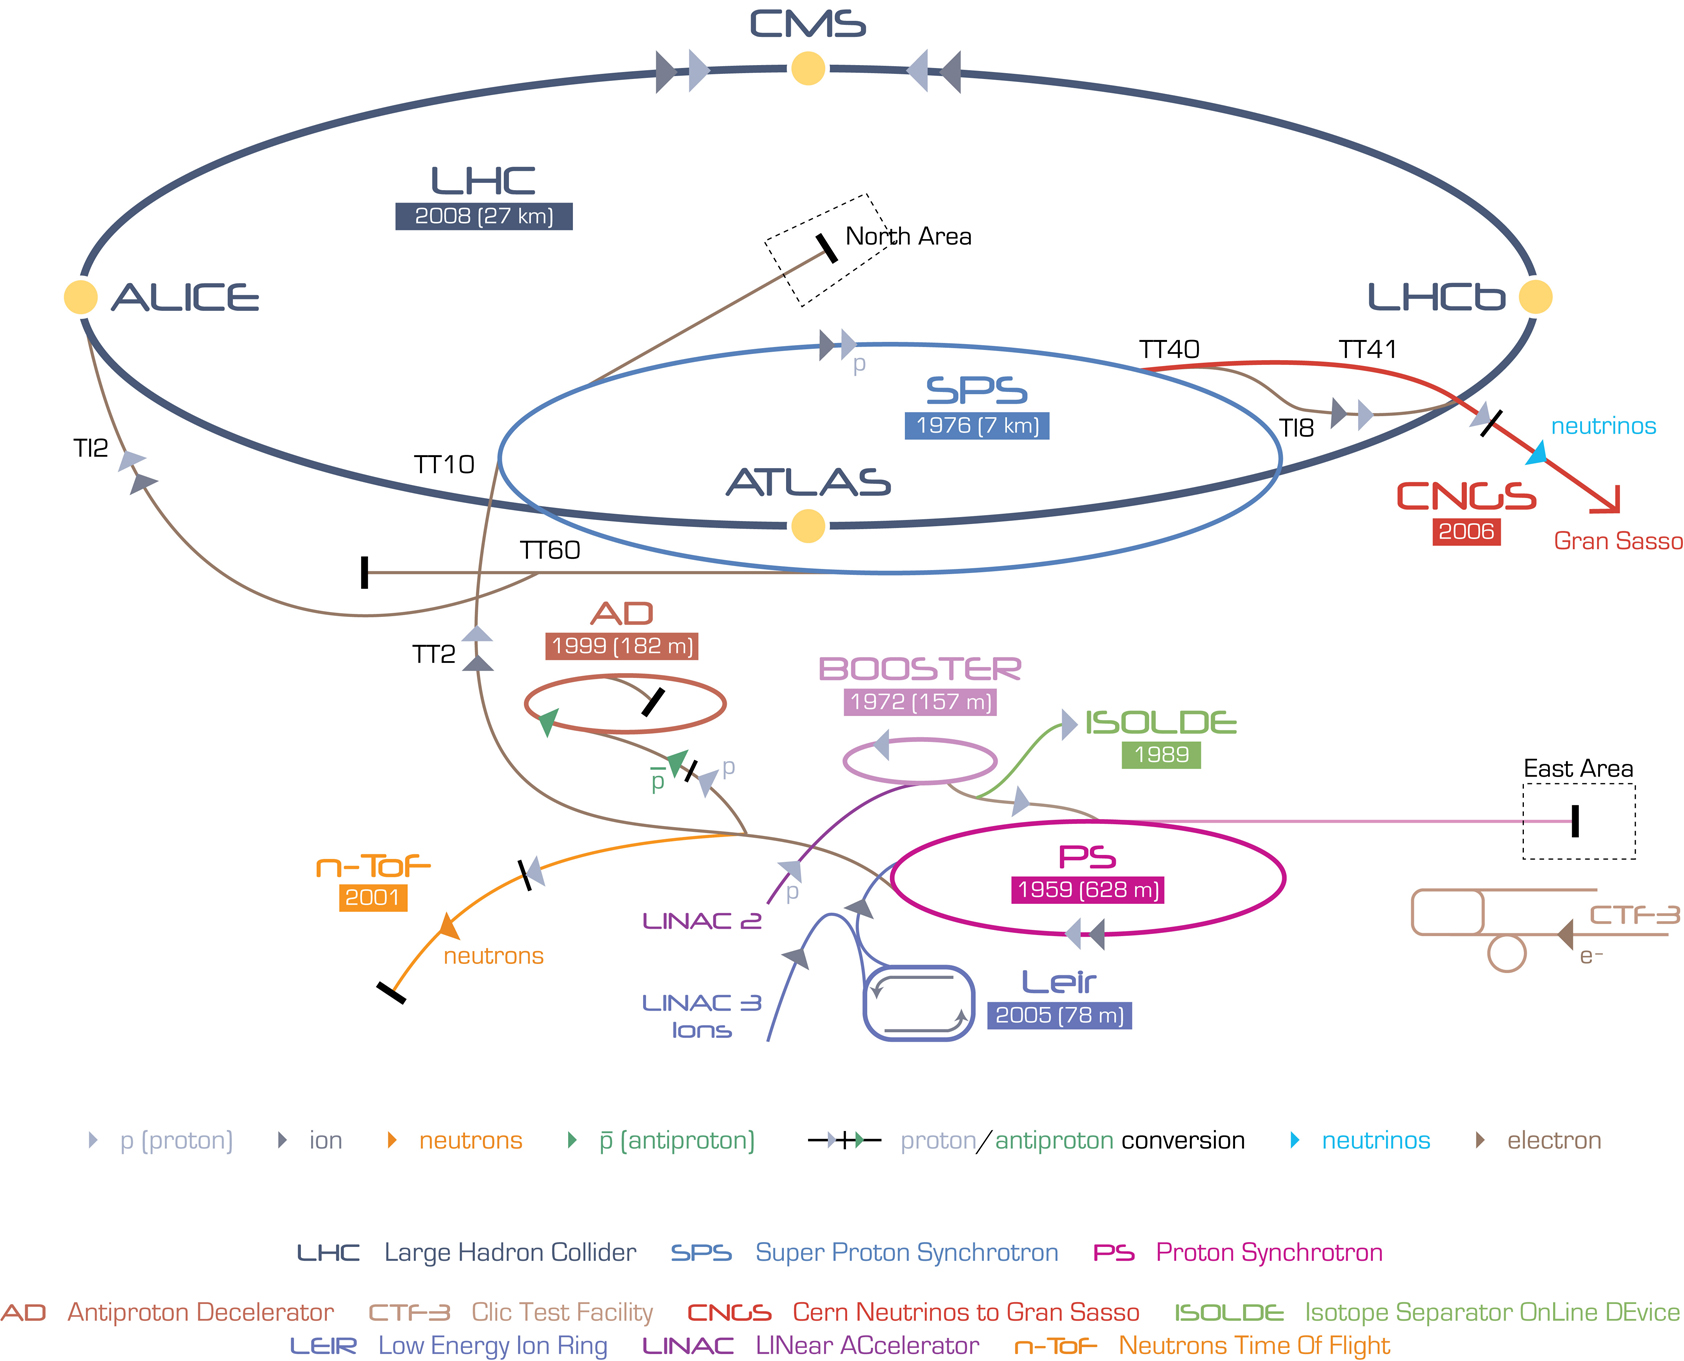
\includegraphics[width=0.7\textwidth]{Figs/machine/Cern-Accelerator-Complex.jpg}
\caption{Schematic diagram of the CERN accelerator complex, showing the various 
accelerators and storage rings, ultimately feeding the Large Hadron Collider.}
\label{fig:cern_acc_complex}
\end{figure}

The beams, consisting of approximately up to 1380 bunches of $\orderof(10^{11})$
protons, are brought into collision
at four points around the LHC ring within specialised detector systems, as shown
in figure~\ref{fig:lhc_diagram}. During the
first run of the LHC, `Run I', bunches were spaced in 50 ns intervals, giving
a bunch crossing rate of 20 MHz. Collisions proceed for a number of hours, 
while collision rates are maintained by scanning the transverse beam positions, 
until such a time when proton numbers are depleted and the beam recycled so that
the fill process can be repeated.

\begin{figure}[ht!]
\centering
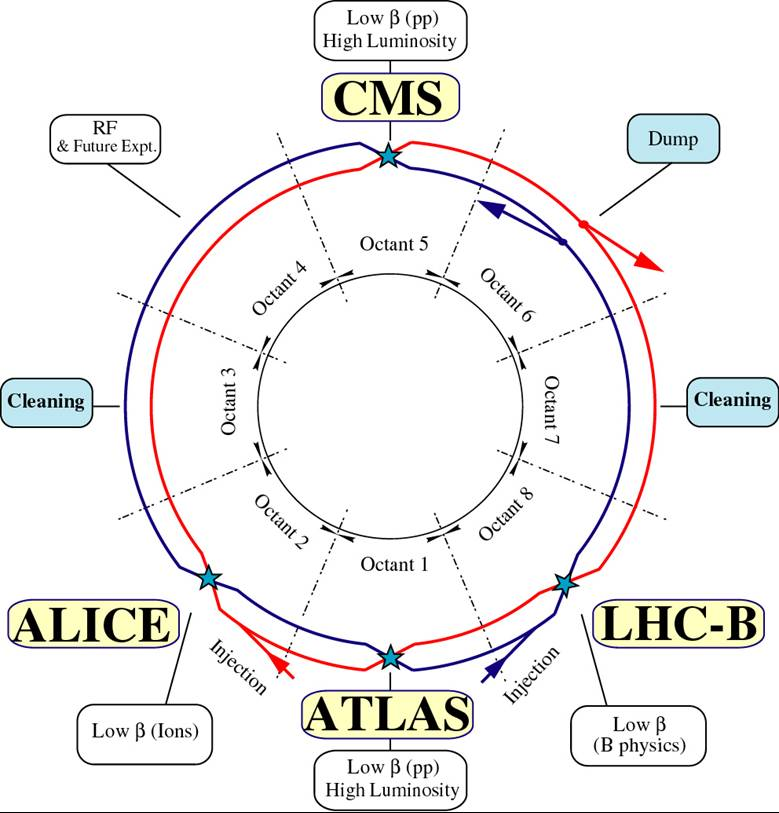
\includegraphics[width=0.5\textwidth]{Figs/machine/lhc-schematic.jpg}
\caption{Schematic diagram of the Large Hadron Collider, indicating the 
positions of the four collision points and their corresponding detector 
experiments.}
\label{fig:lhc_diagram}
\end{figure}


The rate of collisions at each interaction point is described by the 
instantaneous Luminosity, given by the equation:
% 
\begin{equation}
L_{inst.} = \frac{f_{orbit}n_{B}N_p^2}{A_{eff}}
\end{equation}
% 
where $f_{orbit}$ is the orbital frequency of bunches in the LHC, $n_B$ is the 
number of bunches in the machine, $N_p$ is the number of protons per bunch, and 
$A_{eff}$ is the effective area overlap between colliding bunches. The peak 
$L_{inst.}$ per day for CMS is shown in figure~\ref{fig:inst_lumi_day} and the
integral over time is shown in figure~\ref{fig:lumi_2012}, both for the full run
period throughout 2012.

\begin{figure}[h!]
  \centering
  \begin{subfigure}[b]{0.46\textwidth}
    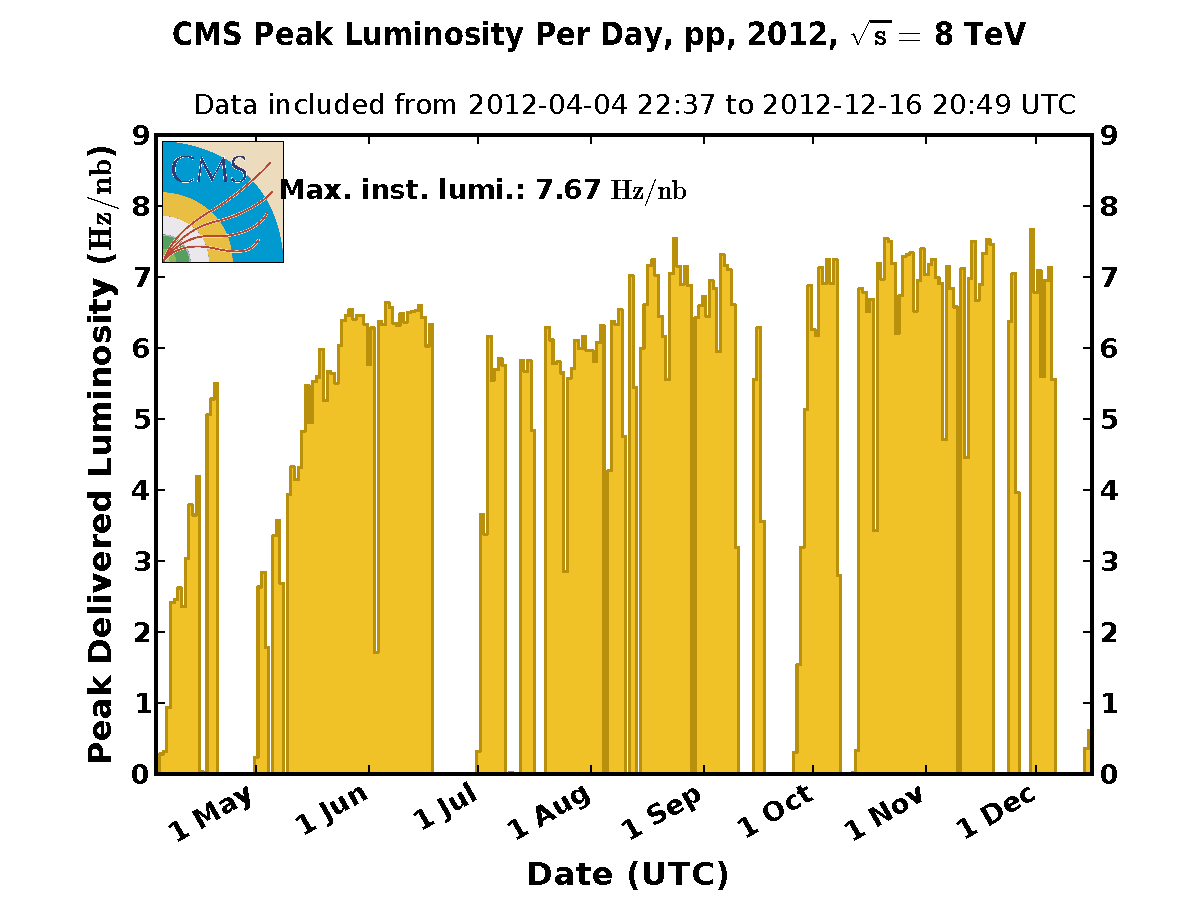
\includegraphics[width=\textwidth]{Figs/machine/peak_lumi_per_day_pp_2012.pdf}
    \caption{}
    \label{fig:inst_lumi_day}
  \end{subfigure}
  \begin{subfigure}[b]{0.46\textwidth}
    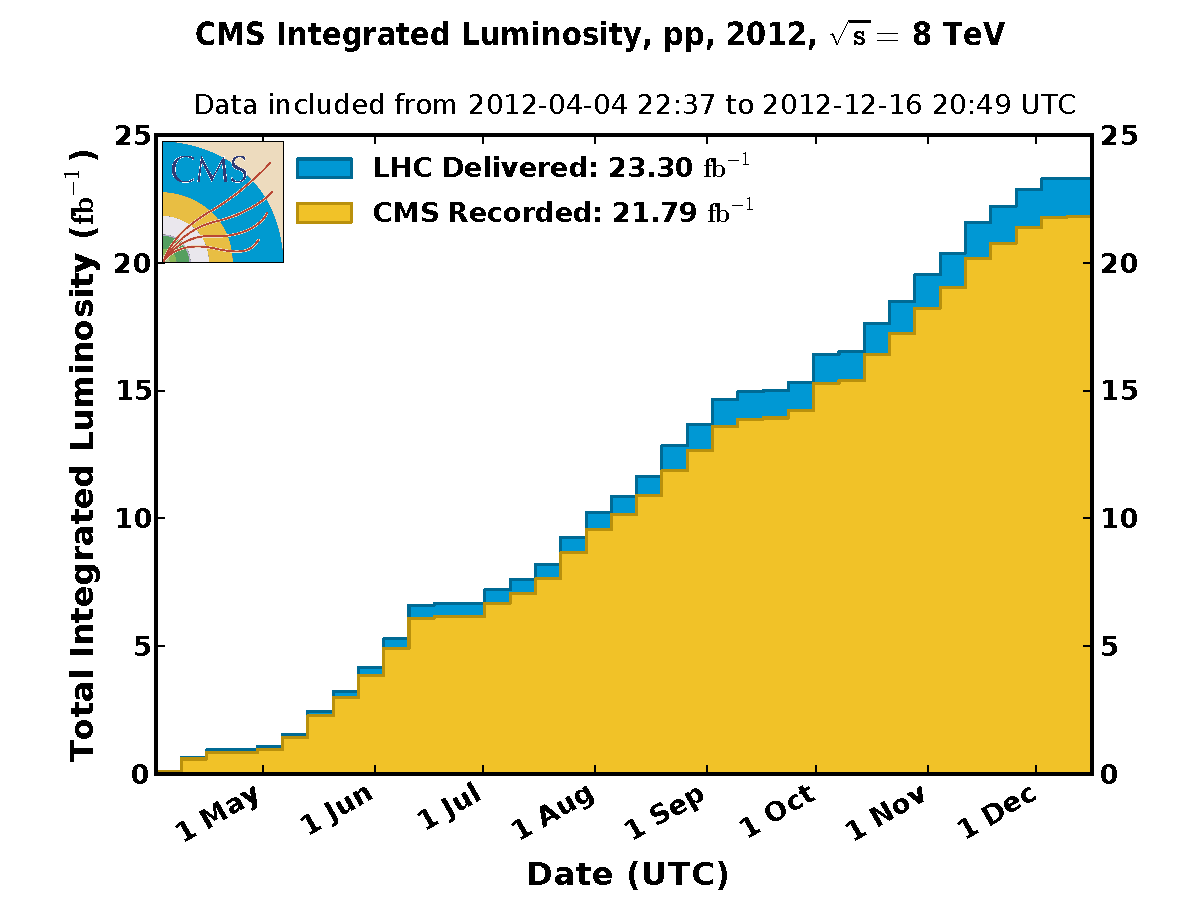
\includegraphics[width=\textwidth]{Figs/machine/int_lumi_per_week_cumulative_pp_2012.pdf}
    \caption{}
    \label{fig:int_lumi_week_cumu}
  \end{subfigure}
  \caption{The peak instantaneous luminosity for each day throughout 2012 
  (a),
  and the integrated luminosity delivered to and recorded at CMS (b)
  from \cite{cmslumi}.}
  \label{fig:lumi_2012}
\end{figure}

\begin{figure}
  \centering
  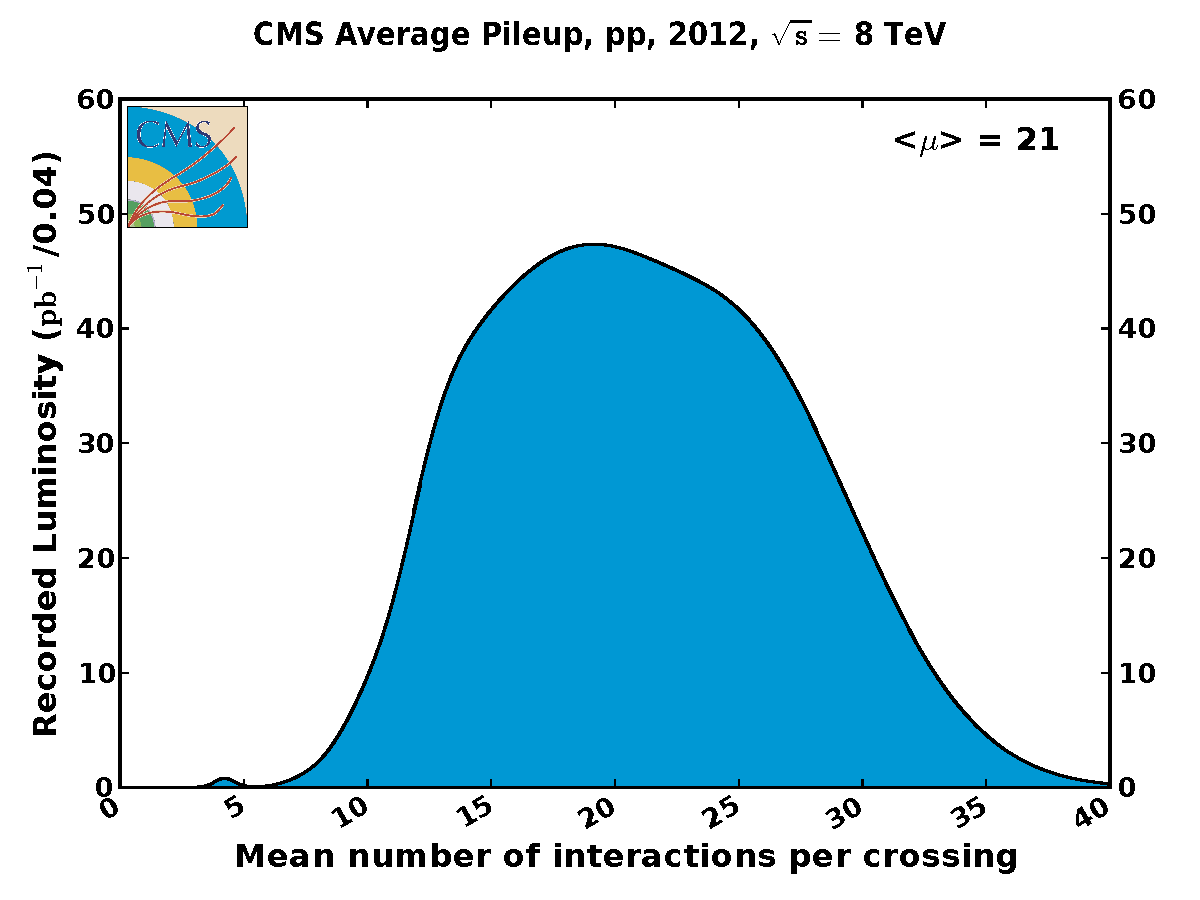
\includegraphics[width=0.6\textwidth]{Figs/machine/pileup_pp_2012.pdf}
  \caption{The average Pileup distribution as seen by the CMS detector
  throughout \runone, taken from \cite{cmslumi}.}
  \label{fig:pileup_runone}
\end{figure}

Simultaneous interactions happening at the time
of each bunch crossing are referred to as in-time pile up (PU), as opposed to 
overlapping particle decays from previous bunch crossings called out-of-time 
pile up (PU). Both phenomena cause significant
experimental challenges for detector readout and event reconstruction.
The average Pileup distribution for \runone is shown in
figure~\ref{fig:pileup_runone}

% The four detectors of the LHC are ALICE, ATLAS, CMS and LHCb. Of these,
% both ATLAS and CMS 
% are considered as general purpose detectors, optimised for the investigation of
% high-\Pt phenomena.

% The work in this thesis uses the CMS detector, which is discussed in 
% the following section.


%********************************** % Second Section  *************************************
\section{Compact Muon Solenoid}  %Section - 1.2 
\label{sec:detector_overview}

The Compact Muon Solenoid (CMS), is a
hermetic detector system (figure~\ref{fig:cms_diagram})
optimised for the study on high-\Pt objects and their decays \cite
{CMSexperiment}.
It is designed to make accurate measurements of the positions and momenta of
physics objects such as electrons, muons, taus,
photons and jets. Owing to an almost complete 4$\pi$ solid angle coverage, CMS is 
capable of also making accurate measurements of global momentum imbalances due
to the presence of weakly interacting particles.

\begin{sidewaysfigure}
  \centering
  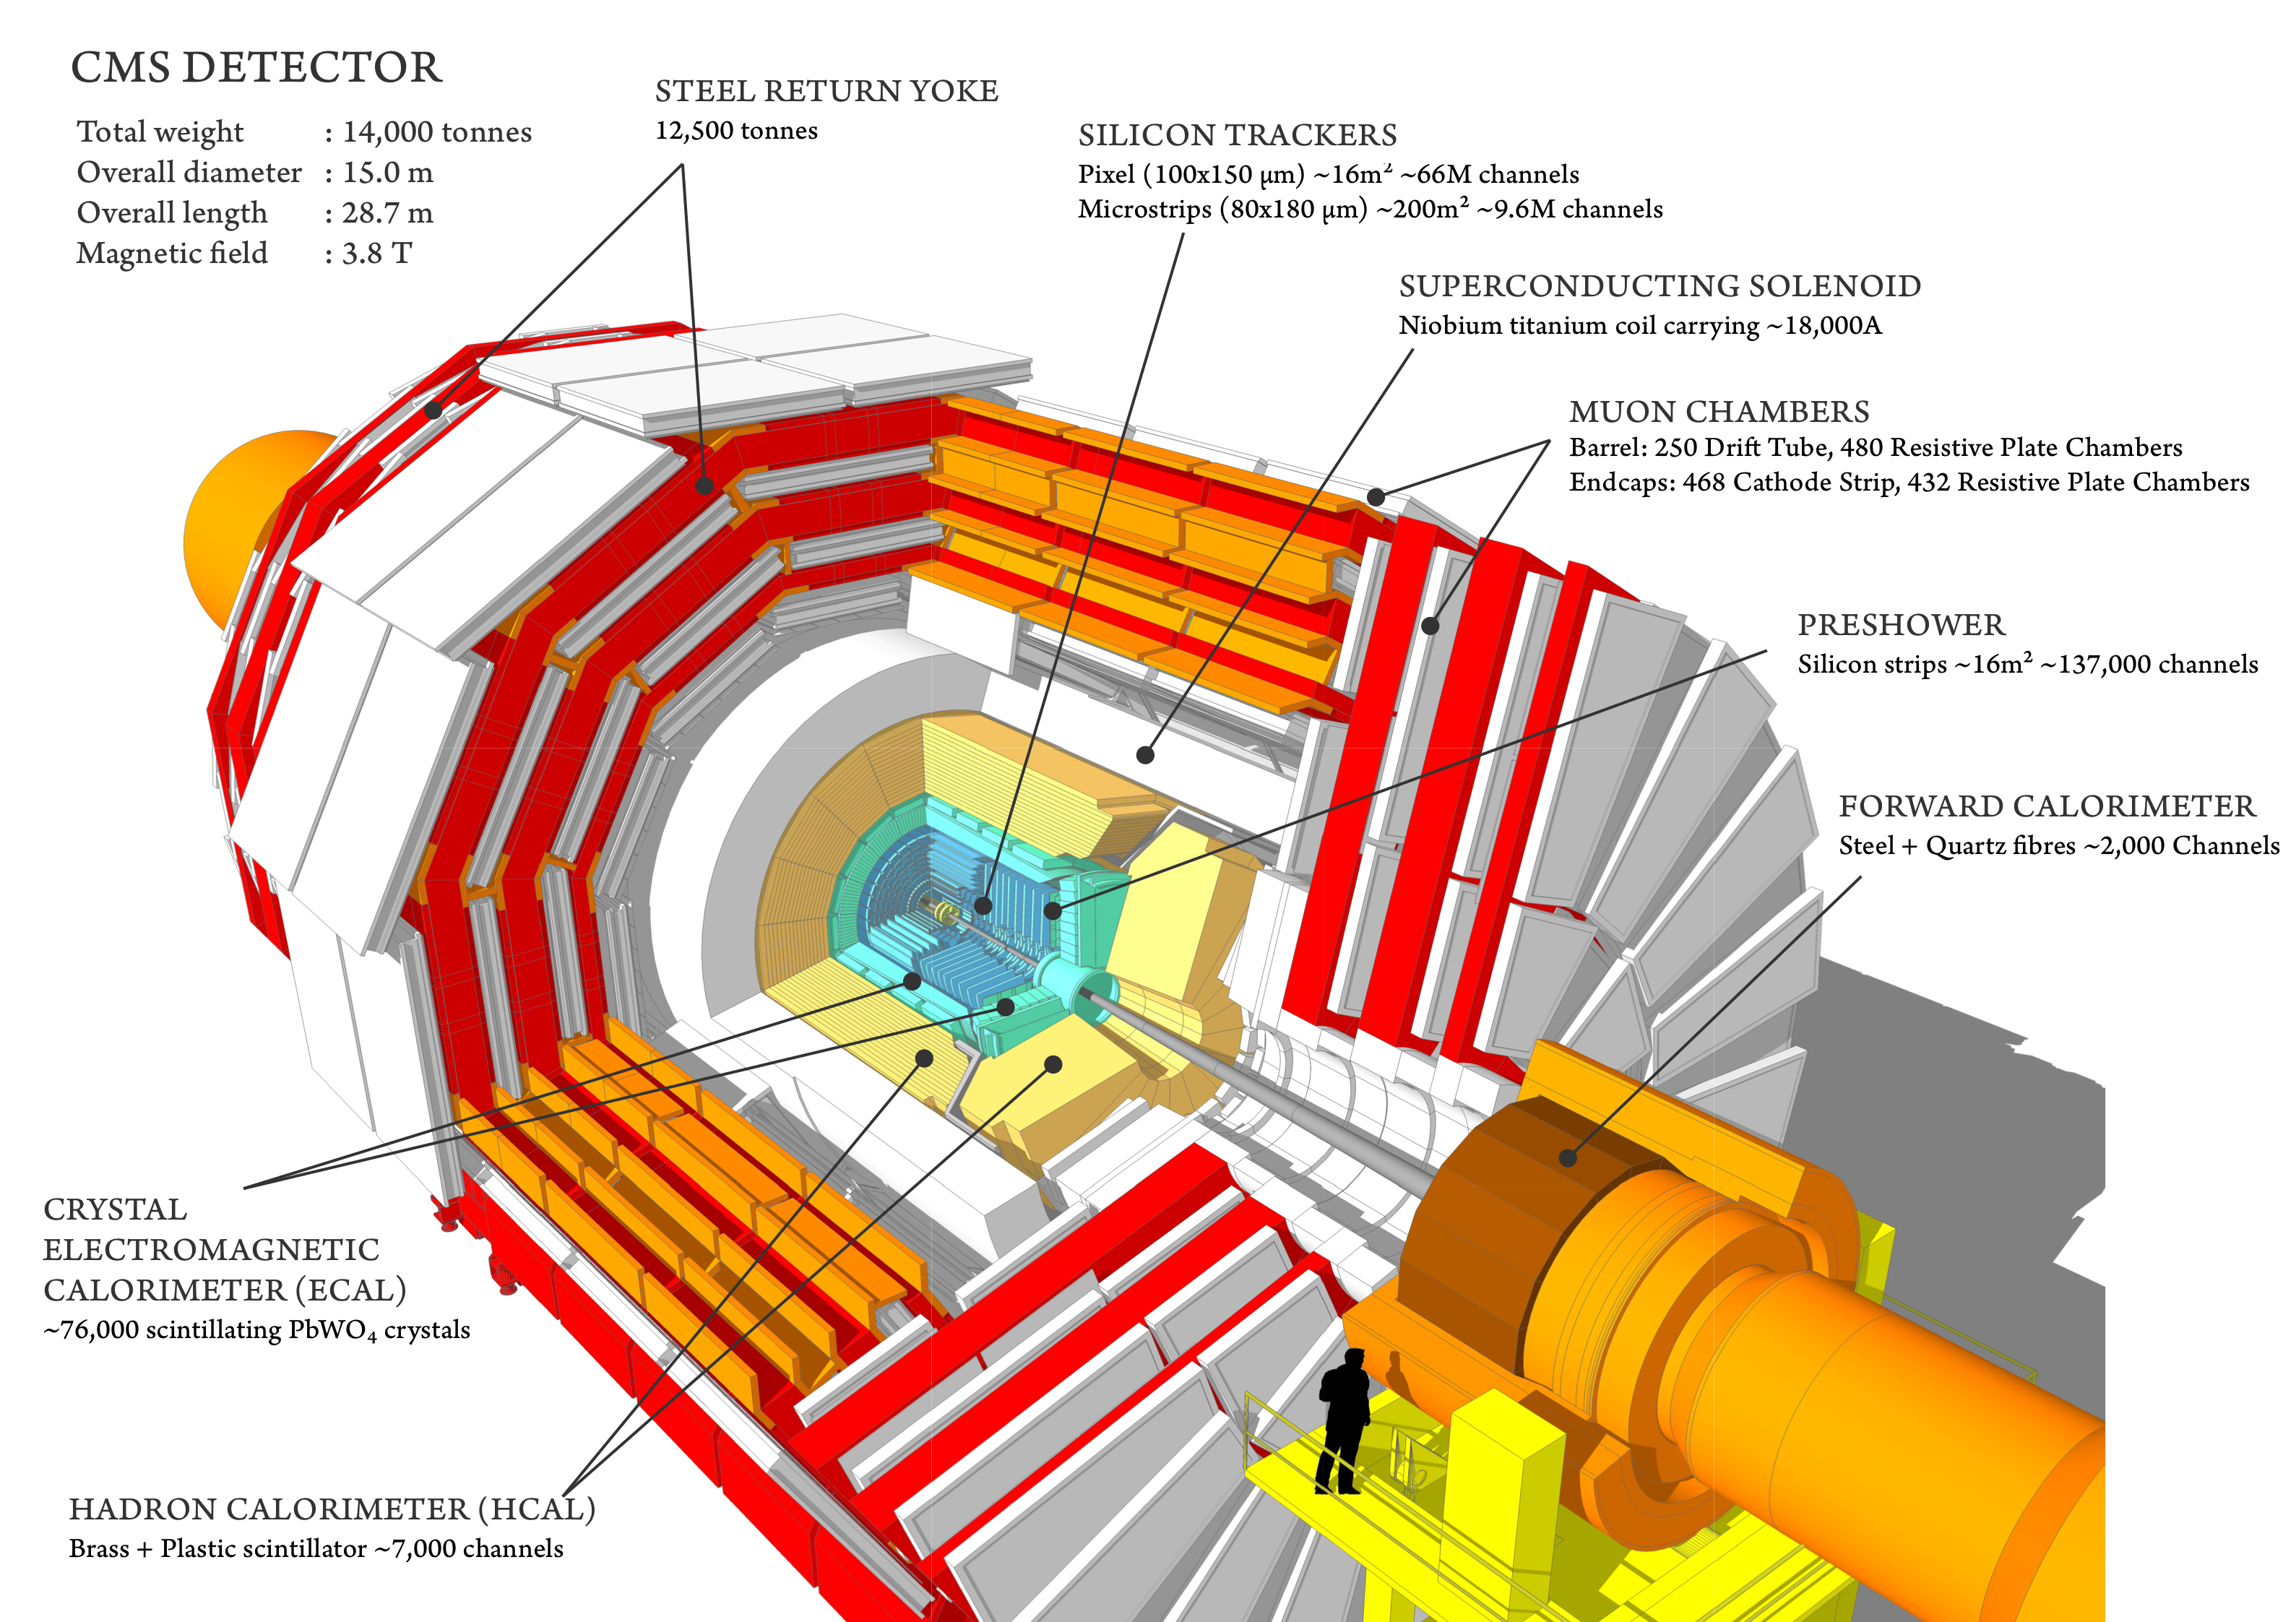
\includegraphics[width=\textwidth]{Figs/machine/cms_120918_02.png}
  \caption{Diagram of the Compact Muon Solenoid taken from
  \cite{Sakuma:2013jqa}.}
  \label{fig:cms_diagram}
\end{sidewaysfigure}

The cylindrical detector is 28 m in length, 15 m in diameter and has a mass of 
around 14,000 tonnes. 
The z-axis is taken to be the longitudinal dimension along the beamline, the
x-axis the perpendicular direction pointing towards the centre of the LHC ring, 
and the y-axis pointing skywards, perpendicular to these forming a right-handed 
co-ordinate system. The transverse plane is taken to be the plane of the x and y
axes.

Directions relative to the CMS detector are described with the variables $\phi$,
the angular direction in the transverse plane with the range $[-\pi, \pi]$, and 
the lorentz-invariant quantity `pseudo-rapidity', $\eta$, describing an angle
with respect to the z-axis, defined as:
% 
\begin{equation}
\eta = - ln \ tan \Bigg( \frac{\theta}{2} \Bigg)
\end{equation}
% 
where $\theta$ is the polar angle between the particle trajectory and the beam
pipe in the y-z plane.
Differences in these two variables, namely $\Delta \phi$ and $\Delta 
\eta$, are invariant under Lorentz boosts, and so can be used to construct a 
furthermore Lorentz-invariant angular separation between particles:
% 
\begin{equation}
\Delta R = \sqrt{ (\Delta \eta)^2 + (\Delta \phi)^2}
\end{equation}
% 
CMS is arranged in a layered configuration of sub-detectors, structured as a 
cylindrical barrel, completed by two end-caps. The barrel contains a
super-conducting solenoid magnet capable of producing a 3.8 T magnetic field. 
Operated at 4.5 K, with a 18.5 kA current, the longitudinal field produced bends
the trajectories of charged particles allowing for precise charge and momenta 
measurements.

%********************************** % Third Section  *************************************
\section{Detector Subsystems}  %Section - 1.3
\label{sec:detector_subsystems}

The layered structure of the CMS subsystems exists in both the barrel and
end-cap regions. The following describe each of the subsystems in more detail.

\subsection{Tracker}
% - inner three layers of pixel detectors
%     - also have end-caps of pixel detectors
% - what type of pixels? what pitch? technology?
% - provide 2d information of hit positions

% - further 10 layers of silicon strip detectors
%     - n-in-p?
%     - and end-

% - this detector system provides information of not only the vertex location and 
% tracking of charged particles, but also given the massive magnet, a 
% determination of both their charge and momenta.

The silicon tracker system consists of inner pixel-based and outer microstrip-
based detectors.

The pixel detector consists of three layers of silicon pixel sensors situated 
as close as 4 cm from the beamline, capable 
of producing 2D hit information of charged particles for use in vertex 
finding with a spatial resolution of $\sim 10 \mymathhyphen 20$\microm. The barrel section
is accompanied by two end-cap pixel detector
disks. Each sensor contains a 52 x 80 grid of 100 \microm x 150 \microm pixels, 
mounted to a lightweight mechanical substrate along with front-end readout 
electronics.

A further 10 layers of silicon microstrip detectors are used to accurately 
reconstruct the track path of charged particles. The sensors collectively cover 
an area of over 200 $\text{m}^2$, are of p-in-n type, and range from 320 \microm
to 500 \microm in thickness and pixel pitch ranging between 80 \microm and 
205 \microm, depending on distance from the beamline. The track path can be used
to determine both the charge and momentum of charged particles, the latter with
a $\Delta \Pt/\Pt$ of $\sim 1 \mymathhyphen 2 \%$ for a 100 \gev
particle.

All silicon detectors situated so close to the interaction point receive
high-doses of radiation, eventually ageing due to the damage inflicted. Subsequently, 
radiation hard sensor and front-end electronics materials and designs have been
selected to mitigate the effects of ageing due to radiation damage.

\subsection{Electromagenetic Calorimeter}

% - ecal made of scintillating lead tungstate (PbWO4) crystals
%     - each crystal is 0.017 x 0.017 (in deltaEta x deltaPhi dimensions), and 23 
%     cm in length
%         -   corresponds to about 25 radition lengths
%         - moliere radius?
%     - super-crystal arrangement?
% - each crystal has a photodetector to determine the level of scintillation light
% produced
%     - avalanche photo-diodes in the barrel, and vacuum photo-triodes in the 
%     endcap region
%     - radiation hardness?
%     - what material?

% - this detector system provides energy and spatial information of
% electromagnetically showering particles.

The Electromagnetic Calorimeter (ECAL) system provides accurate measurements of 
energy deposits and the identification of electromagnetically interacting 
particles, and can also produce spatial measurements when used in conjunction 
with data from the tracker system. The detector consists of scintillating
lead-tungstate
($\text{PbWO}_4$) crystals, each of dimension 0.017 x 0.017 ($\Delta \eta \times
\Delta \phi$) and 23 cm in length, corresponding to around 26 radiation lengths
and providing a Moli\`{e}re radius of 2.2 cm. In both the barrel and the
end-cap regions, individual crystals are clustered into super-towers, to match
with towers in the trigger system (the calorimeter trigger system is described
later in section~\ref{sec:detector_trigger}).

Scintillation light produced in each crystal is collected by either
avalanche photo-diodes in the barrel and vacuum photo-triodes in the
endcap. The detectors are required to be both radiation hard and capable of
operating within the strong magnetic environment of CMS.

The ECAL system is measured as having a $\Delta E/E$ resolution for a 100 \gev
particle of $\sim 0.5\%$, exceeding it's technical design requirements.

\subsection{Hadronic Calorimeter}

% - alternating layers of brass absorber and plastic scintillator
% - scintillators are sectioned into towers, 0.087x0.087 in barrel and 0.17x0.17 
% in the endcaps (double check this isn't just my interpretation of ted's eta 
% numbers)
% - light produced in the scintillator layers is transmitted via wavelength 
% shifting fibres to a hybrid photo-diode for detection

The Hadronic Calorimeter (HCAL) system measures the energy of hadronic showers 
originating from single-quarks and gluons (i.e. jets). It is constructed from
layers of alternating brass absorber and plastic scintillator, of which there
are 17 in the barrel and 19 in the endcaps. The latter are spatially
divided into towers measuring 0.087 x 0.087 in the barrel and end-caps. Hadronic
showers of particles deposit energy as scintillation light in the plastic layers,
which is transmitted via wavelength shifting fibres to be measured in hybrid
photo-diodes. The energy resolution of the HCAL system is calculated with
respect to $\pi$-meson energy reconstruction, and is measured to be
$\sim 90\%/\sqrt{E}$ in the barrel, and $\sim 100\%/\sqrt{E}$ in the endcap.

% \emph{can i ignore the HF region, as we ignore forward jets?}

\subsection{Muon Systems}

% - comprised of three different gaseous detector technologies, each with 
% different coverages in eta
% - drift tubes (DT)
%   - traditional technology, optimised for low occupancy
%   - central: eta < 1.2
% - cathode strip chambers (CSC)
%   - designed for high magnetic field and neutron backgrounds
%   - forward: 0.9 < eta < 2.4
% - resistive plate chambers (RPC)
%   - designed for high magnetic field and neutron backgrounds
%   - forward and central eta < 2.1

The muon system provides identification and precision measurements of
muon position and momenta. Energy deposits in the muon systems can be combined
with corresponding information from the tracker to improve momentum resolution
significantly. It is designed to have an energy resolution, $\Delta \Pt/\Pt$ of
$\sim10\%$ on it's own, and $\sim2\%$ when combined with tracker information,
both measured for muons with \Pt < 100 \gev.

\begin{figure}[ht!]
\centering
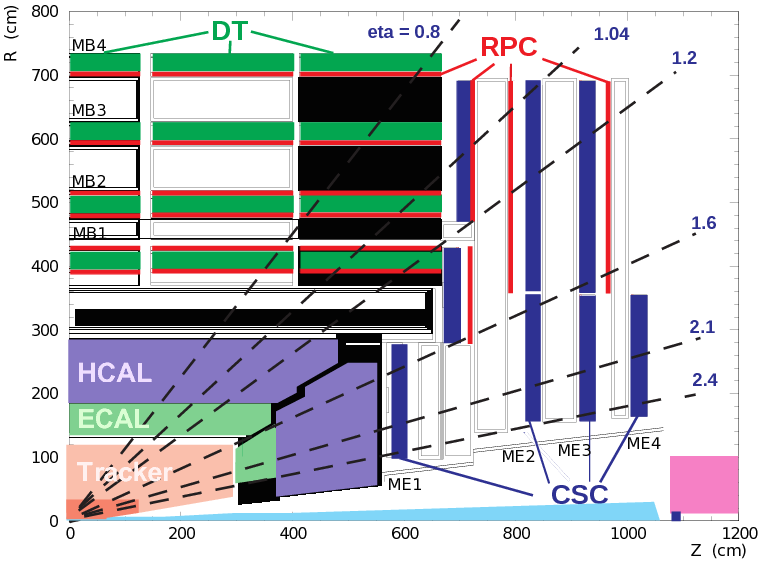
\includegraphics[width=0.6\textwidth]{Figs/machine/pictures_MuonSys-mod3.png}
\caption{Cross section of the CMS detector in the y-z plane, showing the three 
muon systems as well as other interior sub-detector systems.}
\label{fig:muon_system_diagram}
\end{figure}

Muons are detected in the outer layers of the detector, with the muon system 
comprised of three different gaseous detector technologies each with different 
pseudo-rapidity coverage, shown in figure~\ref{fig:muon_system_diagram}. The
central barrel region, $|\eta|<1.2$ is equipped with 
Drift Tube (DT) detectors - a traditional detector technology, optimised for low
-occupancy measurements. Cathode Strip Chambers (CSC) cover the forward region,
$0.9 < |\eta| < 2.4$, and dual-layered Resistive Plate Chambers (RPC) cover
$|\eta| < 2.1$ - both CSC and RPC detectors being optimised for operation in 
the presence of both high magnetic field and neutron background environments.

%********************************** % Fourth Section  *************************************
\section{Trigger and Data Acquisition}  %Section - 1.4
\label{sec:detector_trigger}

\subsection{Trigger system}
Events of interest are selected using a dedicated triggering system \cite{tridasTDR},
split into two distinct stages: the hardware-based Level-1 Trigger (L1) and
the software-based High-Level Trigger (HLT).

\subsubsection{Level-1 Hardware Trigger}
% - L1 system is hardware based running at a rate of 40 MHz
% - runs on coarse trigger primitive objects, constructed from raw energy deposits
% in the calorimeter and muon systems independently
%     - takes regional information from both the calorimeter and muon systems 
%     independently.
%     - combines regional data in the GCT/GMT
%     - feeds combined objects (from across entire detector) into the GT, where a 
%     L1 accept is made or not.
% \emph{can talk in more detail here about the calorimeter trigger path and the 
% GCT's job}
% - has approximately 3microsecs per events
% - objects considered at L1 are electrons, muons, jets (central and forward) and 
% energy sums (ETT, MET, HTT, MHT)
% - L1Accept is made dependent on the objects within an event meeting 1 of 127 (
% check!) simple threshold and multiplicity based requirements.
% - maximum available output bandwidth of the L1 system is 100 kHz, although the 
% output rate is kept lower than this to allow for stochastic fluctuations

The L1 system consists of a staged, modular design of custom built hardware 
electronics subsystems, as shown in figure~\ref{fig:l1_diagram}. 
The L1 trigger reconstructs energy deposits in the calorimeter and muon systems
into coarse `trigger-primitive' physics objects.
Regional information is gathered by separate modules 
before being combined in the Global Calorimeter Trigger (GCT) and Global Muon 
Trigger (GMT) systems, where physics objects are sorted according to energy. 
Finally, event objects are passed on to the Global Trigger (GT) where a 
`Level-1 Accept' (L1A) signal is issued or not, dependent on the event meeting 
one of up to 128 simple object threshold and multiplicity based requirements.

\begin{figure}[ht!]
  \centering
  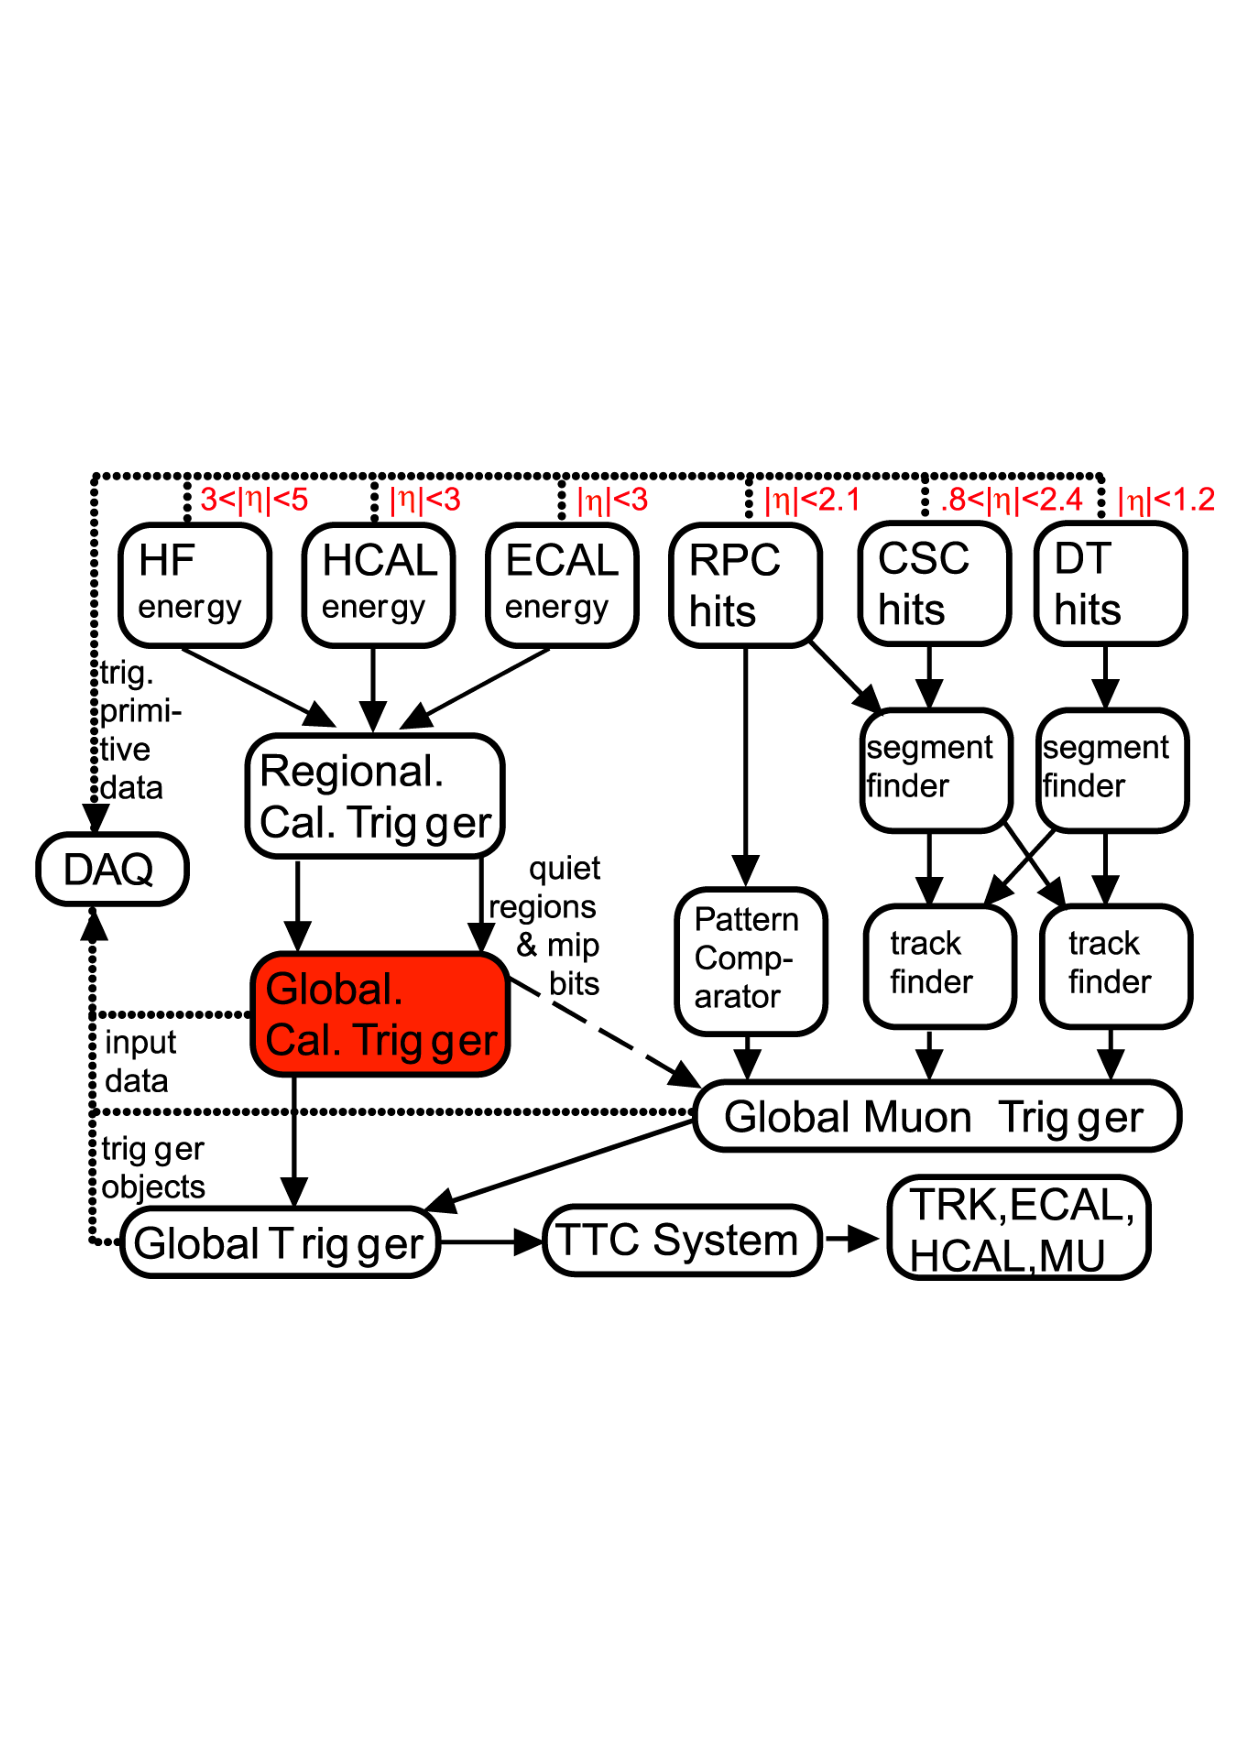
\includegraphics[width = 0.55\textwidth]{Figs/machine/L1_diagram.pdf}
  \caption{Schematic overview of the Level-1 hardware trigger system of CMS. $
  \eta$ coverage is shown in red and the data-flow indicated by arrow 
  direction.}
  \label{fig:l1_diagram}
\end{figure}

The L1 system is required to run at 40 MHz, equal to the maximal bunch-crossing
rate within CMS, with a L1A decision required within a latency of 3 $\mu s$. The
maximum available output bandwidth of the L1 system is 100 kHz, but typically is
maintained at a lower value to allow for stochastic rate fluctuations.

\subsubsection{High-level Trigger}
% - Following a L1A signal, candidate events are optically transmitted to the high
% level trigger, consisting of a large computer farm of the off the shelf server 
% PCs
% - events are reconstructed/built in more detail
% - passed on to a suite of analyst-designed software triggers which can 
% reconstruct more advanced objects and event variables, such as alphaT (as 
% described later in chapter BLAH) - has approximately 50ms per event
% - HLT reduces rate to around 300 events per second

Following a L1A signal, candidate events are optically transmitted to the HLT 
system, consisting of a large computer farm of server 
PCs. Due to the increase in available processing time of up to 50 ms, events can
be reconstructed in greater detail allowing for a closer emulation of offline 
reconstruction techniques. Complex analyst-designed trigger rules are used, 
which can employ more sophisticated event-level variables such as \alphat
(described in detail later in chapter~\ref{ch:5}).

The HLT reduces the event rate further by around two orders of magnitude,
producing an output event rate of up to 1 kHz. Events passing the HLT are
transmitted to Grid system \cite{Eck:840543} for full offline reconstruction.

\chapter{Object Definitions}
\label{ch:objects}

% **************************** Define Graphics Path **************************
\ifpdf
    \graphicspath{{Chapter4/Figs/Raster/}{Chapter4/Figs/PDF/}{Chapter4/Figs/}}
\else
    \graphicspath{{Chapter4/Figs/Vector/}{Chapter4/Figs/}}
\fi


%********************************** % First Section  *************************************

Physics objects are observed as energy deposits in the various detector 
subsystems throughout CMS. Specific definitions for the different 
objects used in this analysis are provided by the Physics Object Groups (\emph{POGs})
and are described in the following sections.


%********************************** % Second Section  *************************************
\section{Jets}  %Section - 1.2
\label{sec:objects_jets}

Jets are produced through the hadronisation and showering of a single quark or gluon 
through the calorimeter systems.Energy deposits 
are clustered using the anti-$k_T$ algorithm \cite{antikt} with
an $R=0.5$ cone size parameter. Jets are reconstructed from
calorimeter information and are widely known as `Calojets'. While many analyses use
`Particle Flow' (PF) techniques to reconstruct `PFJets' - jets constructed using information
from combinations of multiple sub-detector systems - this analysis continues to use `Calojets'
for compatibility with our well studied, Calojet-based signal triggers.
Table~\ref{tab:jet_id_loose} summarises the ID requirements used in this 
analysis, which correspond to the ``Loose'' working point \cite{ref:jet-id}.
% The raw energy measurements are subject to 
% effects from overlapping pp collisions (PU), therefore corrections are made to
% account for this . Clustered jets 
% are also corrected to establish a uniform response in $\eta$ and \Pt
% .
% Energy deposits clustered into jet objects are corrected to ensure a
% good translation between measured energy and parton energy.
Raw energy measurements that form jets have the following sequential
corrections \cite{ref:jet-jes, 2011JInst...611002C} applied:
\begin{description}
\item[L1] To remove energy originating from PU events, therefore removing any
dependence on luminosity across a dataset \cite{Cacciari2008119, 1126-6708-2008-04-005}.
\item[L2] To ensure a uniform energy response in $\eta$ across the calorimeter \cite{Chatrchyan:2011ds}.
\item[L3] To ensure a uniform response according to the \Pt of the deposit \cite{Chatrchyan:2011ds}.
\item[L2L3] Final, additional corrections to bring data and MC into agreement.
\end{description}


\begin{table}[!ht]
  \caption{Criteria for the ``loose'' jet identification working point.\label
  {tab:jet_id_loose}}
  \footnotesize
  \begin{center}
    \begin{tabular}{ll}
      \hline
      \hline
      Requirement                & Description                                                      \\
      \hline
      f$_{HPD} < 0.98$           & Fractional contribution from the ``hottest'' Hybrid Photo Diode. \\
      f$_{EM} > 0.01$            & Minimum electromagnetic fractional component.                    \\
      N$^{90}_{\rm hits} \geq$ 2 & Number of HCAL channels containing at least
      90\% of total energy.      \\
      \hline
      \hline
    \end{tabular}
  \end{center}
\end{table}


\subsection{Identification jets from b quarks}

Jets originating from b quarks can be identified using information from the 
vertex detector due to their increased lifetime with respect to gluons, light
flavour quarks (u, d, s) or charm quarks. 
B tagging algorithms are designed to determine the probability that a jet 
originates from a b quark, given, amongst other properties, the track
displacement from the primary vertex (PV). Each algorithm
calculates a value used to discriminate between a jet originating from a
b quark or other sources.

The Combined Secondary Vertex (CSV) algorithm \cite{CMS-PAS-BTV-12-001} is used
in this analysis. The distribution of discriminator values is shown in
Figure~\ref {fig:btag_csv_discrim}.
The ``Medium'' working point corresponds to a discriminator
threshold of $>0.679$, and is used in this analysis. This working point
corresponds
to a mistag rate for gluons/light-quarks of 1\%, and a pT dependent efficiency
in the range of 60-70\%, as shown in Figure~\ref{fig:btag_csv_eff}. Also
shown in Figure~\ref{fig:btag_csv_eff} are the MC scale factors, $SF_b$, defined
as the ratio of the CSV b tagging algorithm efficiency in data and MC, to be
applied to MC samples.

\begin{figure}[h!]
  \centering
  \begin{subfigure}[b]{0.46\textwidth}
    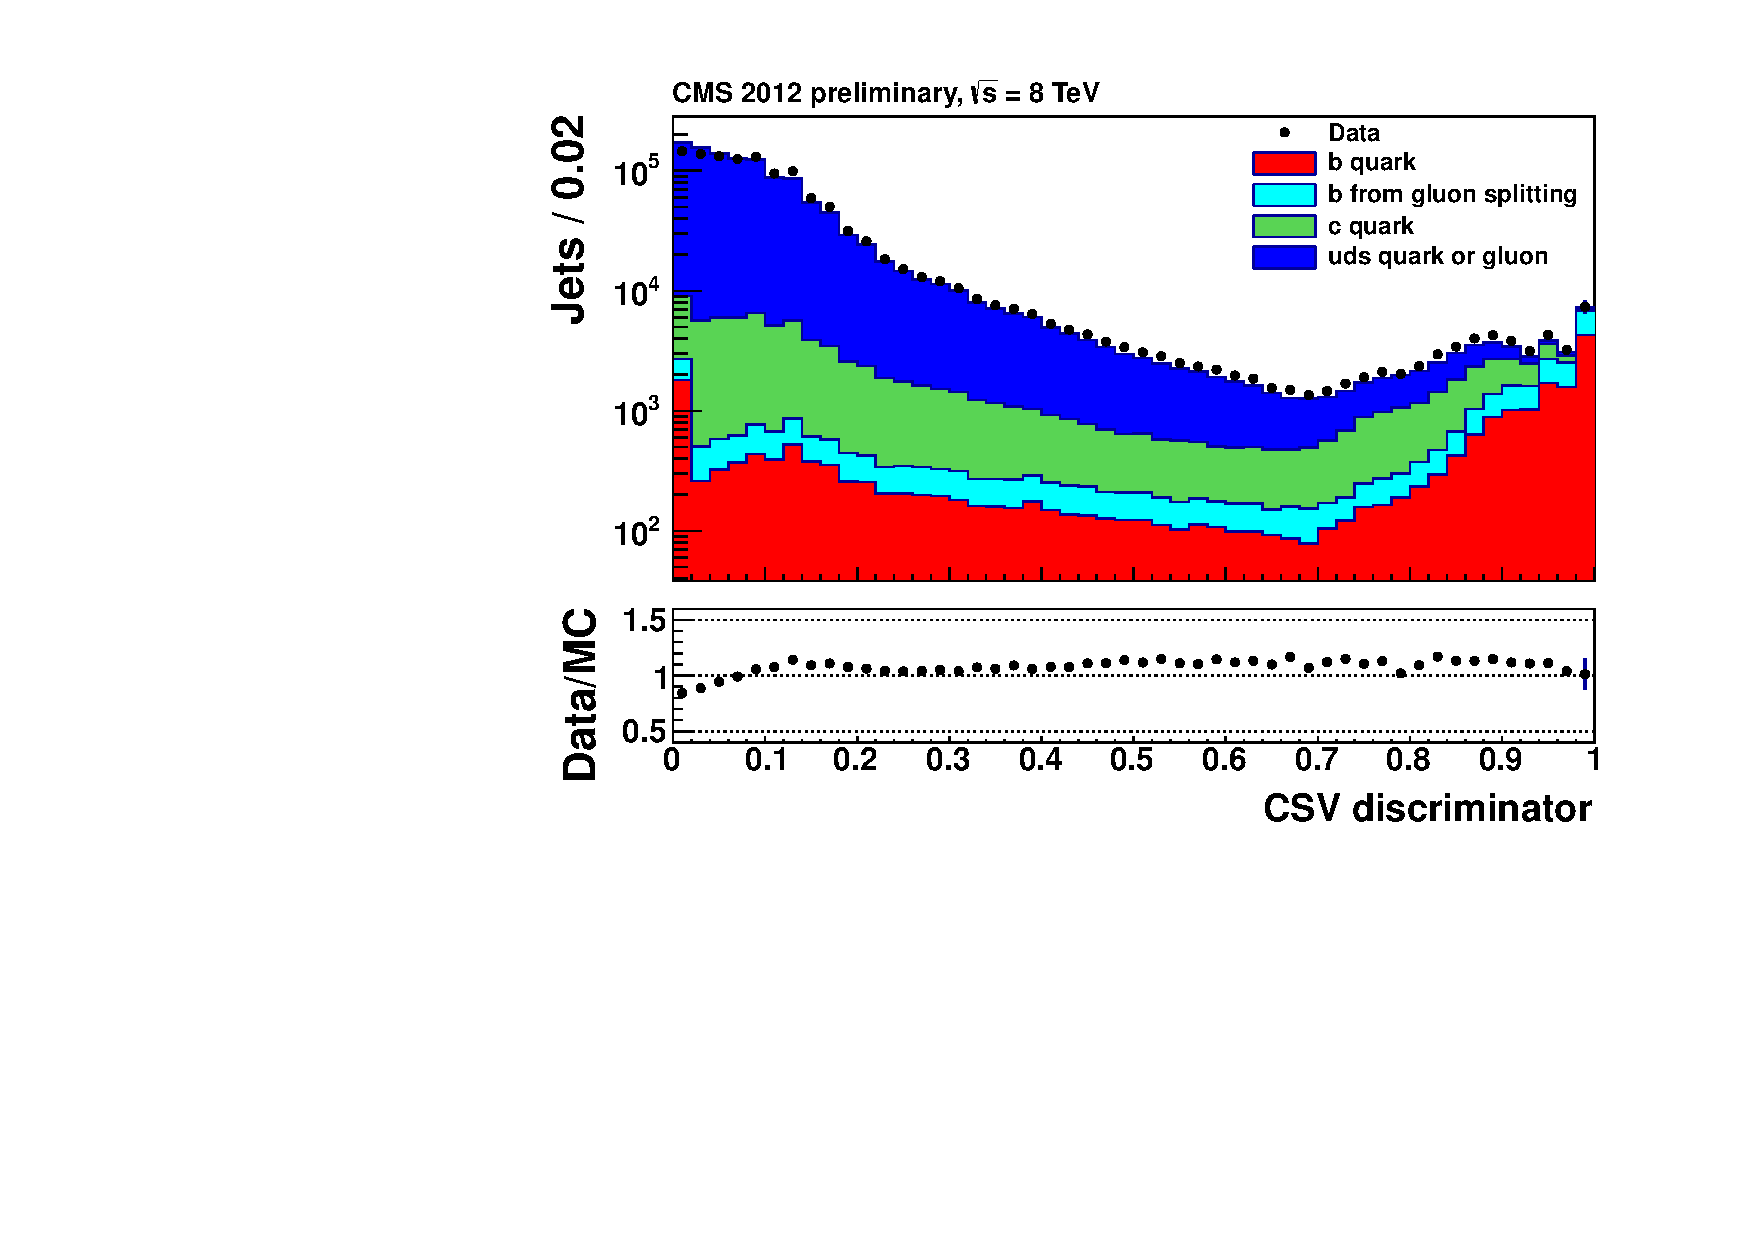
\includegraphics[width=\textwidth]{Figs/btag/csv_discrim.pdf}
    \caption{CSV Discriminator}
    \label{fig:btag_csv_discrim}
  \end{subfigure}
  \begin{subfigure}[b]{0.46\textwidth}
    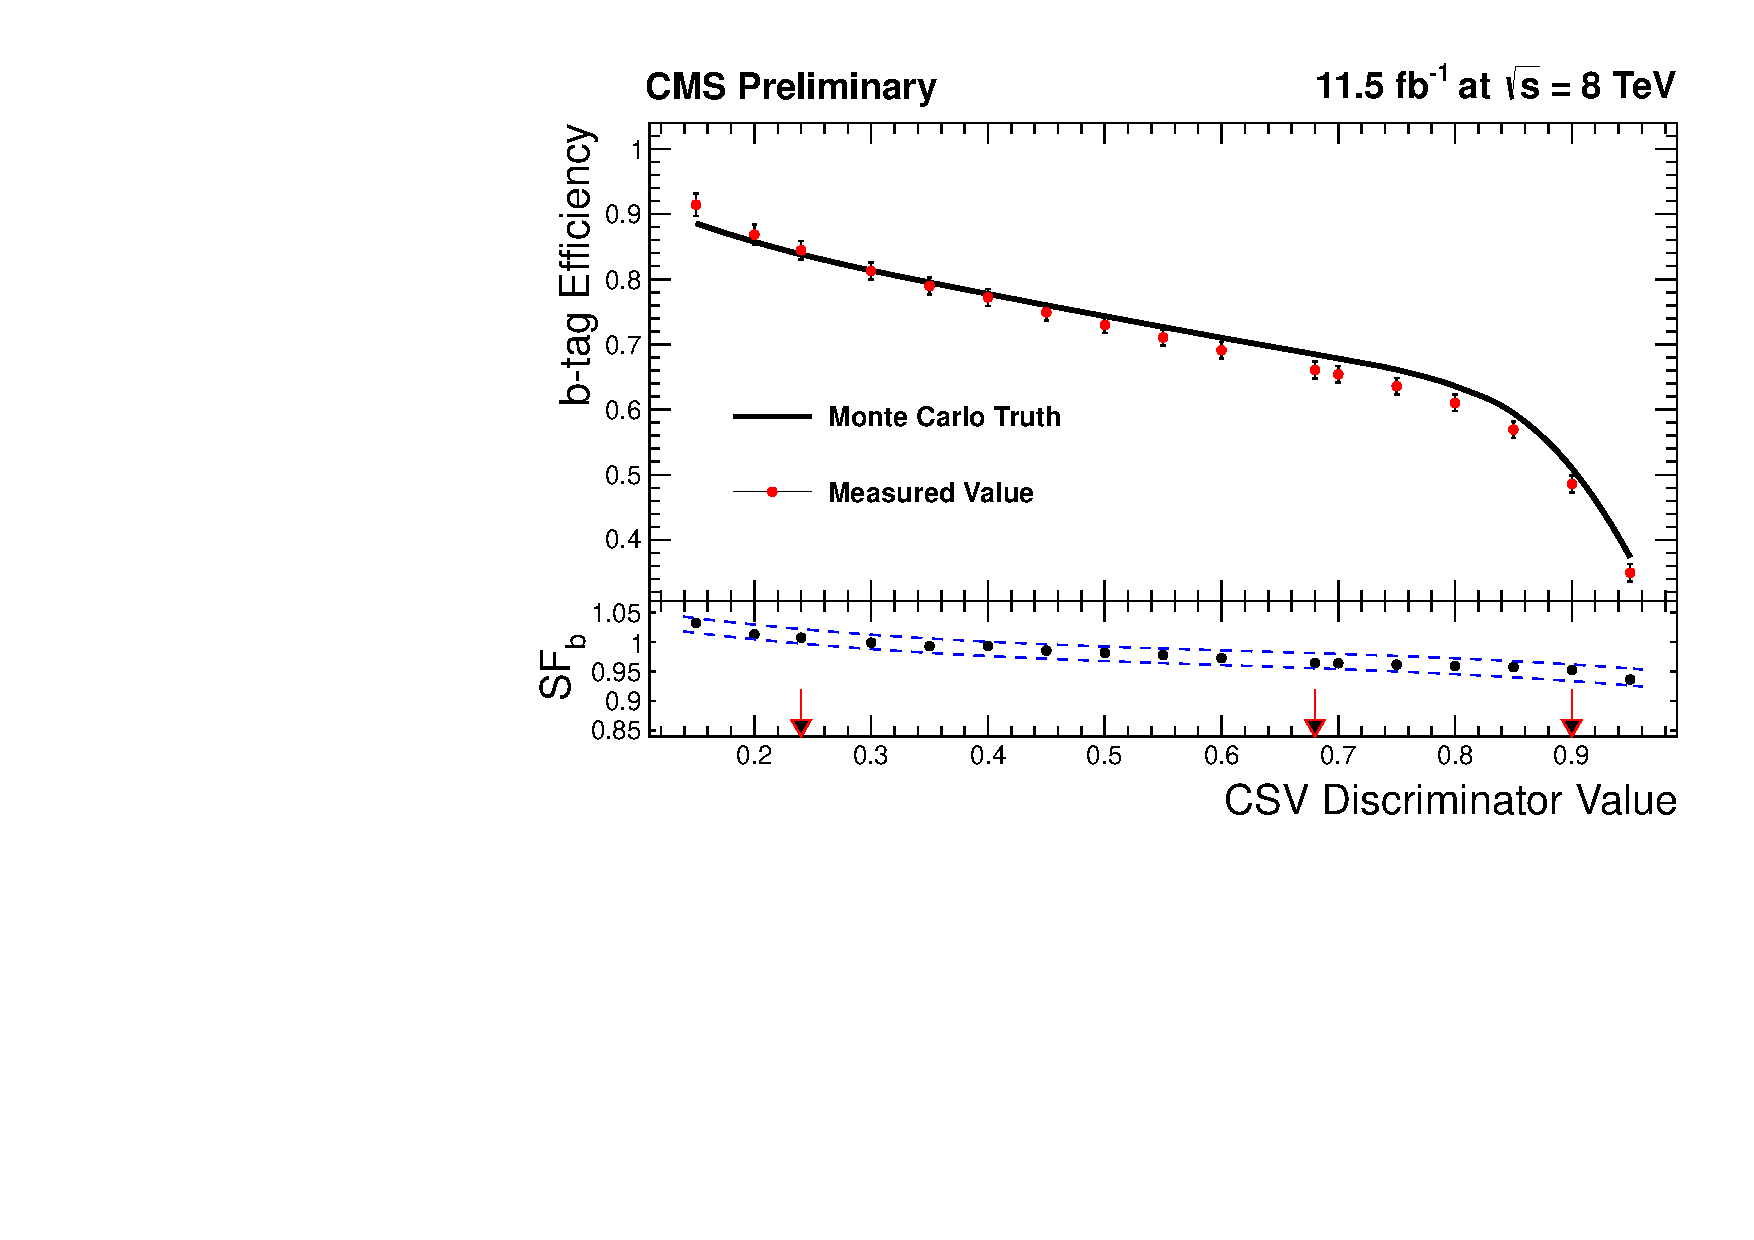
\includegraphics[width=\textwidth]{Figs/btag/csv_eff.pdf}
    \caption{CSV Efficiency}
    \label{fig:btag_csv_eff}
  \end{subfigure}
  \caption{The Combined Secondary Vertex b tagging algorithm discriminator
  distribution (left) and the b tagging efficiency (right) as measured in both
  data and simulation. MC scale factors are shown in the lower plot of
  \ref{fig:btag_csv_eff} \cite{CMS-PAS-BTV-13-001}.}
  \label{fig:btag_csv}
\end{figure}

%********************************** % Fourth Section  *************************************
\section{Muons}  %Section - 1.4
\label{sec:objects_muons}
Muons are identified from energy deposits predominantly in the muon systems and
the tracker using the muon \emph {POG's} Tight working point definition
\cite{ref:muon-id}, as summarised in Table~\ref{tab:muon-id}. This definition is
used in both the muon selection in the \mj and \mmj control regions, and the
muon veto in the hadronic signal region.
% 
\begin{table}[ht!]
  \caption{Muon identification (Tight working point).\label{tab:muon-id}}
  \centering
  \scriptsize
  \begin{tabular}{ lcp{8.7cm} }
    \hline
    \hline
    Variable & Requirement & Description \\
    \hline
    Global Muon                            & True      & Muon object 
    is reconstructed from both hits in the muon systems and matched hits in the 
    silicon tracker \\
    PFMuon                                 & True      & Muon object reconstructed
    with multiple subsystems using Particle Flow techniques\\ $\chi^{2}
    /ndof$ of fit & $<10$ & Goodness of fit
    of the global muon track fit. Suppresses hadronic punch-through and muons 
    decaying in flight.\\
    Muon chamber hits                      & $>0$      & At least 1 hit in a 
    muon chamber. Suppresses hadronic punch-through and muons 
    decaying in flight.\\
    Muon station hits                      & $>1$      & Muon hits in at least 2
    muon stations. Suppresses punch-through and accidental track-to-segment matches.
    Also makes consistent with trigger muon requirements. \\
    Transverse impact $d_{xy}$             & $<0.2$ mm & Tracker track is close 
    to Primary Vertex in the x-y plane. Helps suppress cosmic ray muons and muons 
    from decays in flight. \\
    Longitudinal distance $d_{z}$              & $<0.5$ mm & Tracker track is
    close 
    to Primary Vertex in z-direction. Suppresses muons from cosmic rays, decays in flight 
    and PU. \\
    Pixel hits                             & $>0$      & At least 1 pixel hit. 
    Suppresses muons from decays in flight. \\
    Track layer hits                       & $>5$      & Guarantees good \Pt 
    measurement. \\
    PF Isolation (PU corrected) & $<0.12$   & Particle Flow based 
    isolation, based on a cone size of $\Delta R < 0.4$, with ``$\Delta \beta$'' 
    PU corrections applied. \\
    \hline
    \hline
  \end{tabular}
\end{table}

%********************************** % Fifth Section  *************************************
\section{Photons}  %Section - 1.5
\label{sec:objects_photons}

Photon definitions are made relative to their position in the ECAL,
either
in the barrel or the endcap, as summarised in Table~\ref{tab:photon-id-egamma}. 
This Tight working point ID is defined by the \emph{POG} group
\cite{ref:photonidtwiki} and used for both the photon
selection in the \gj control region and as a veto in the hadronic signal region.

\begin{table}[t]
  \caption{Photon identification (Tight working point).\label{tab:photon-id-egamma}}
  \centering
  \scriptsize
  \begin{tabular}{ cccp{4.2cm} }
    \hline
    \hline
    Categories                    & Barrel                             & Endcap
    & Description                         \\
    \hline
    % Conversion safe electron veto & Yes                                & Yes &
% https://twiki.cern.ch/twiki/bin/viewauth/CMS/ConversionTools#Conversion_safe_electron_veto_fo  \\
    Single Tower H/E              & < 0.05                               & < 0.05                               
    & Ratio of energy deposited in the HCAL towers within $\Delta R<0.15$ of the ECAL 
    supercluster, and the ECAL supercluster itself. \\
    $\sigma_{i\eta i\eta}$        & < 0.11                               & < 0.31 & 
    The cluster shape covariance of the ECAL supercluster in the $\eta$
    dimension. \\
    &&&\multirow{4}{4.4cm}{PF-based isolation requirements to ensure no hadronic
    or electromagnetic 
    activity with a cone defined by $\Delta R < 0.3$. The isolation is
    corrected for PU effects.}\\
    PF charged hadron isolation   & < 0.70                               & < 0.50                               & \\
    PF neutral hadron isolation   & < 0.4 + 0.04 $\times$ $\Pt^{\gamma}$  & < 1.5 + 0.04 $\times$ $\Pt^{\gamma}$&
    \\
    PF photon isolation           & < 0.5 + 0.005 $\times$ $\Pt^{\gamma}$ & < 1.0 + 0.005 $\times$ $\Pt^{\gamma}$& \\
    \\
    \\
    \hline
    \hline
  \end{tabular}
\end{table}

%********************************** % Third Section  *************************************
\section{Electrons}  %Section - 1.3
\label{sec:objects_electrons}
The Electron \emph{POGs} Loose working point ID \cite{ref:electronidtwiki} is
used in this analysis to veto 
electrons from all areas of the analysis. This cut based identification is 
defined separately for the barrel and endcap regions of the detector, uses
information
from the calorimeter systems as well as the tracker, and is
summarised in Table~\ref{tab:ele-id}. The final two requirements are
specifically for the rejection of electrons originating from photons converted
into $e^-e^+$ pairs.

\begin{table}[h]
  \caption{Electron identification (Loose working point).\label{tab:ele-id}}
  \centering
  \scriptsize
  \begin{tabular}{ lccp{8.8cm} }
    \hline
    \hline
    Categories                                               & Barrel    &
    Endcap    & 
    Description \\
    \hline
    $\Delta \eta_{In}$                                       & < 0.007     &
    < 0.009     & 
    The difference between the track and ECAL supercluster in the $\eta$ dimension. \\
    $\Delta \phi_{In}$                                       & < 0.15      &
    < 0.10      &
    The difference between the track and ECAL supercluster in the $\phi$ dimension. \\
    $\sigma_{i\eta i\eta}$                                   & < 0.01      &
    < 0.03      & 
    The cluster shape covariance of the ECAL supercluster in the $\eta$ dimension. \\
    H/E                                                      & < 0.12      & < 0.10      &
    Ratio of energy deposited in the HCAL towers within $\Delta R<0.15$ of the ECAL 
    supercluster and the ECAL supercluster itself. \\
    d0 (vtx)                                                 & < 0.02      & < 0.02      &
    The transverse distance of the track from the PV. \\
    dZ (vtx)                                                 & < 0.2       & < 0.20      &
    The longitudinal distance of the track from the PV. \\
    $\lvert(1/E_{\textrm{ECAL}} - 1/p_{\textrm{trk}})\rvert$ & < 0.05      & < 0.05      &
    Comparison of the ECAL supercluster energy and the track \Pt, to suppress
    low \Pt fakes. \\
    PF relative isolation                                    & < 0.15      & 0< .15      &
    PF based isolation calculated from particle activity within a cone of
    $\Delta R < 0.3$. \\
    Vertex fit probability                                   & 10$^{-6}$ & 10$^{-6}$ &
    Probability of fit to potential conversion tracks. \\
    Missing hits                                             & $\leq1$         & $\leq1$         &
    Number of missing tracker hits due to possible conversion. \\
    \hline
    \hline
  \end{tabular}
\end{table}

%********************************** % Sixth Section  *************************************
\section{Energy Sums}  %Section - 1.6
\label{sec:objects_energy_sums}
Physics objects are combined in the form of kinematic variables
known as energy sums. The definitions of the energy sum variables are:
% 
\begin{equation}
    \begin{split}
    \Et = \sum_{i}^{} |\Ptvect_i| , \\
    \met = -\big|\sum_{i}^{} \Ptvect_i\big| , \\
    \HT = \sum_{i}^{\textrm{jets}} |\Ptvect_i| , \\
    \mhtvect = -\sum_{i}^{\textrm{jets}} \Ptvect_i, \\
    \mht = -\big|\sum_{i}^{\textrm{jets}} \Ptvect_i\big|; \\
    \end{split}
\label{eq:energy_sums}
\end{equation}
% 
namely the total transverse energy, total missing transverse energy (`MET'), total transverse
hadronic energy, total missing transverse energy vector and total missing transverse hadronic energy (`MHT').
These are calculated on the fly in the analysis using identified objects,
with the exception of \met which is constructed from PF candidates and subject to type-I
corrections (jets used for \met calculation are subject to prescribed Jet Energy
Corrections themselves). A full set of \met filters are defined by the MET \emph{POG} as
summarised in Table~\ref{tab:met_filters}. The filters account for various
physics and detector effects which can give un-physical or spurious \met 
signals.

\begin{table}[b!]
  \caption{\met filters employed in the analysis, as recommended by the MET \emph{POG}.}
  \label{tab:met_filters}
  \centering
  \scriptsize
  \begin{tabular}{ lp{11.2cm} }
    \hline
    \hline
    Filter Name & Description \\
    \hline
    Beam Halo CSC ID        & Beam interactions with residual gases in the beam pipe
    or with mechanical apertures, causing secondary particle production. Events 
    are vetoed if an event contains a positive beam halo ID from the CSC
    detectors. \\ \\
    HBHE Noise              & Noise originating from instrumentation issues with
    the HCAL's Hybrid Photo Diodes (HPDs) or the Readout Boxes (RBXs). Events are
    vetoed if they contain isolated clusters of noisy cells in either the barrel 
    or endcap.\\ \\
    Tracking Failure        & Significant energy deposits in the calorimeter 
    systems with no corresponding tracks due to tracker algorithm failure. 
    Events are vetoed if the summed \Pt of all tracks in the event is  equal to less than 
    10\% of the \HT.\\ \\
    HCAL Laser Misfire      & Calibration lasers being accidentally fired 
    through the HCAL during bunch crossings (as opposed to abort gaps). Events 
    are removed that contain such accidental laser firings. \\ \\
    DeadECAL Cell TP        & Dead or damaged ECAL crystals which cannot read 
    out energy deposits correctly. Trigger primitives are checked to determine 
    how much energy was lost, and events are appropriately masked. \\
    \hline
    \hline
  \end{tabular}
\end{table}

The \met variable only appears in the analysis in the calculation of the transverse
mass of the lepton system in the \mj control region (Section~\ref{sec:mujets_control_sample})
and in the \mhtmet variable (Section~\ref{sec:qcd_cleaning_below_thresh}) as an independent
estimator of the event's missing energy.

%********************************** % Seventh Section  *************************************
\section{Single Isolated Tracks}  %Section - 1.7
\label{sec:objects_sit}
Single Isolated Tracks are used to identify hadronically decaying $\tau$ leptons
and leptonically decaying W bosons where the corresponding lepton has failed
identification for whatever reason.
Summarised in Table~\ref{tab:sit-id}, the selection is based on PF
candidates. This ID is used as
a veto in all selections, with the selected `tag' lepton ignored in the \mj and
\mmj control selections. The ID definition is taken from \cite{singleleptonstop}.

\begin{table}[ht!]
  \caption{Single Isolated Track identification.\label{tab:sit-id}}
  \centering
  \scriptsize
  \begin{tabular}{ lcp{8.6cm} }
    \hline
    \hline
    Variable & Requirement & Description \\
    \hline
    Charge                      & $\neq 0$      & Candidate is charged. \\
    Track \Pt                   & $> 10$~\gev   & Track transverse momentum. \\
    $\Delta z(track, PV)$       & $<0.05$~cm     & Longitudinal distance of
    track
    from primary vertex. \\
    Relative Track Isolation    & $<0.1$        & Isolation relative to other PF 
    candidate tracks in cone of $\Delta R <0.3$ \\
    \hline
    \hline
  \end{tabular}
\end{table}

\chapter{The \alphat Analysis}
\label{ch:analysis}

% **************************** Define Graphics Path **************************
\ifpdf
    \graphicspath{{Chapter5/Figs/Raster/}{Chapter5/Figs/PDF/}{Chapter5/Figs/}}
\else
    \graphicspath{{Chapter5/Figs/Vector/}{Chapter5/Figs/}}
\fi


%********************************** % First Section  *************************************
\section{Analysis Overview}  %Section - 1.1 
\label{sec:selection_analysis_overview}

Analyses searching in the jets and \met final state encounter significant 
backgrounds from SM sources of both genuine and fake \met. Genuine \met 
originates from W and Z boson production, decaying with one or more neutrinos in
the final state. In this analysis background predictions are made for these
processes using 
extrapolations into the signal region from independent, process-specific control
samples, as described in chapter~\ref{ch:background}.
Fake \met predominantly is found due to mismeasurements of QCD 
multijet (MJ) events, which is the dominant process in the hadronic environment
and 
phase space considered in this analysis due to it's very large cross section. 
Small inconsistencies in the handling of such large backgrounds or rare detector
effects can therefore 
have a significant impact on an analysis. This background is reduced to an 
entirely negligible level using the dimensionless kinematic variable, \alphat
(described in section~\ref{sec:alphat}).

% OLD
% Analyses searching in the jets and \met final state encounter significant 
% backgrounds from SM sources of both genuine \met, originating from the leptonic 
% decays of W bosons, 
% and fake \met, originating from jet mis-measurement. The \alphat 
% analysis makes predictions for the former using a data-driven transfer factor 
% technique to extrapolate yields from statistically independent control samples 
% into the signal region. However the latter, sources of fake \met from QCD multijet events,
% are reduced to a negligible level using the kinematic 
% variable \alphat.

In this analysis events are binned in exclusive categories of \HT, 
and the multiplicity of jets and b-tagged jets,  
\nj and \nb, as summarised in table~\ref{tab:ht-bins}. Such binning allows for
targeted interpretations across the vast array of
possible simplified model final states, while reducing background yields to a 
minimum.

\begin{table}[ht!]
  \caption{\HT bin lower bounds used for each \nj and \nb category.\label
  {tab:ht-bins}}
  \centering
  \small
  \begin{tabular}{ lrrrrrrrrrrr }
    \hline
    \hline
    (\nj,\nb)       & \multicolumn{11}{c}{\HT bins (\gev)}                                                                                \\
    \hline
    (2-3,0)           & 200 & 275 & 325 & 375 & 475 & 575 & 675 & 775 & 875 & 975 & $>$1075  \\
    (2-3,1)           & 200 & 275 & 325 & 375 & 475 & 575 & 675 & 775 & 875 & 975 & $>$1075  \\
    (2-3,2)           & 200 & 275 & 325 & 375 & 475 & 575 & 675 & 775 & $>$875   & \multicolumn{2}{c}{} \\
%    (2-3,3)          & 200 & 275 & 325 & 375 & 475 & 575 & 675 & 775 & $>$875   & \multicolumn{2}{c}{} \\
    ($\geq$4,0)       & 200 & 275 & 325 & 375 & 475 & 575 & 675 & 775 & 875 & 975 & $>$1075  \\
    ($\geq$4,1)       & 200 & 275 & 325 & 375 & 475 & 575 & 675 & 775 & 875 & 975 & $>$1075  \\
    ($\geq$4,2)       & 200 & 275 & 325 & 375 & 475 & 575 & 675 & 775 & $>$875   & \multicolumn{2}{c}{} \\
    ($\geq$4,3)       & 200 & 275 & 325 & 375 & 475 & 575 & 675 & 775 & $>$875   & \multicolumn{2}{c}{} \\
    ($\geq$4,$\geq$4) & 200 & 275 & 325 & $>$375   & \multicolumn{7}{c}{}                                                        \\
    \hline
    \hline
  \end{tabular}
\end{table}

The main analysis signal region is described in the remainder of this chapter.


\subsection{The \alphat kinematic variable}
\label{sec:alphat}

% QCD multijet (MJ) events dominate the SM background in any search with multiple jets 
% in the final state. Jet energy mis-measurements in a 
% purely QCD MJ event can lead to non-negligible amounts of \mht, therefore 
% passing the signal selection.
Attempting to accurately measure the QCD contribution to the total background is
made very difficult given the hadronic environment of the LHC, and the lack of 
precise measurements and calculations of the large multijet cross sections. As an 
alternative approach, the goal of this analysis is to reduce QCD down to an
entirely negligible level through the use of the dimensionless kinematic
variable, \alphat. The di-jet variable
$\alpha$ was first proposed by Randall et al. in 2008 \cite{Randall:2008rw},
and later translated into the transverse plane for use with LHC analyses
\cite{CMS:2008vya, CMS-PAS-SUS-09-001}.
\alphat is defined for di-jets as:
% 
\begin{equation}
\alphat = \frac{ \sqrt{E_T^{j_2}/E_T^{j_1}} }{ \sqrt{2(1-cos(\Delta \phi))} } ,
\label{eq:alphat_di-jet}
\end{equation}
% 
where $E_T^{j_1}$ and $E_T^{j_2}$ are the reconstructed transverse energies of 
the first and second jets respectively, and $\Delta \phi$ is the seperation 
between the two jets in the $\phi$ plane.

A perfectly measured di-jet event containing back to back jets in $\phi$ of equal energy will
have an \alphat value of 0.5, whereas 
events with \met originating from jet energy mismeasurements will have values of $\alphat<0.5$.
Only events containing sources of genuine \met, whether from SM or BSM sources,
can have values of $\alphat > 0.5$.
% 
% \begin{equation}
% \alphat = \frac{E_T^{j_2}}{M_T} = \frac{\sqrt{}}
% \label{eq:alphat_di-jet}
% \end{equation}
% 
% where $E_T^{j_2}$ is the transverse energy of the less energetic jet and $M_T$ 
% is the transverse mass of the di-jet system, defined as:
% 
% \begin{equation}
% M_T = \sqrt{\bigg(\sum^2_{i=1}{E_T^{j_i}}\bigg)^2 - \bigg(\sum^2_{i=1}{p_x^{j_i}}\bigg)^2 - \bigg(\sum^2_{i=1}{p_y^{j_i}}\bigg)^2}
% \label{eq:mt}
% \end{equation}
% 
% where $E_T^{j_i}$, $p_x^{j_i}$ and $p_y^{j_i}$ are the transverse energy and 
% transverse momentum in the $x$ and $y$ planes, for the jet $j_i$.

The \alphat variable can be generalised to an n-jet case by considering the event as a 
pseudo-di-jet system, constructing each pseudo-jet such that the difference in \HT
between each pseudo-jet system, \deltaHT, is minimised. \alphat then takes the 
form:
% 
\begin{equation}
\alphat = \frac{1}{2} \times \frac{\HT-\deltaHT}{\sqrt{\HT^2 - \mht^2}} = 
\frac{1}{2} \times \frac{1-\frac{\deltaHT}{\HT}}{\sqrt{1 - \big(\frac{\mht}
{\HT}\big)^2}}.
\label{eq:alphat_njet}
\end{equation}
% 

The \alphat variable introduces a correlation between the two variables of \mht
and \deltaHT. This relationship is demonstrated in figure~\ref{fig:alphat_corr}
by the black contours of constant \alphat. The different physics sources
will populate various regions of this plane. Most notably QCD exhibits a strong
correlation between the two variables at low \alphat values
(figure~\ref{fig:alphat_corr_qcd}), while processes with real \met break this
correlation, sitting also at higher values of \alphat
(figures~\ref{fig:alphat_corr_zinv} and \ref{fig:alphat_corr_t2cc}).

\begin{figure}[h!]
  \centering
  \begin{subfigure}[b]{.46\textwidth}
    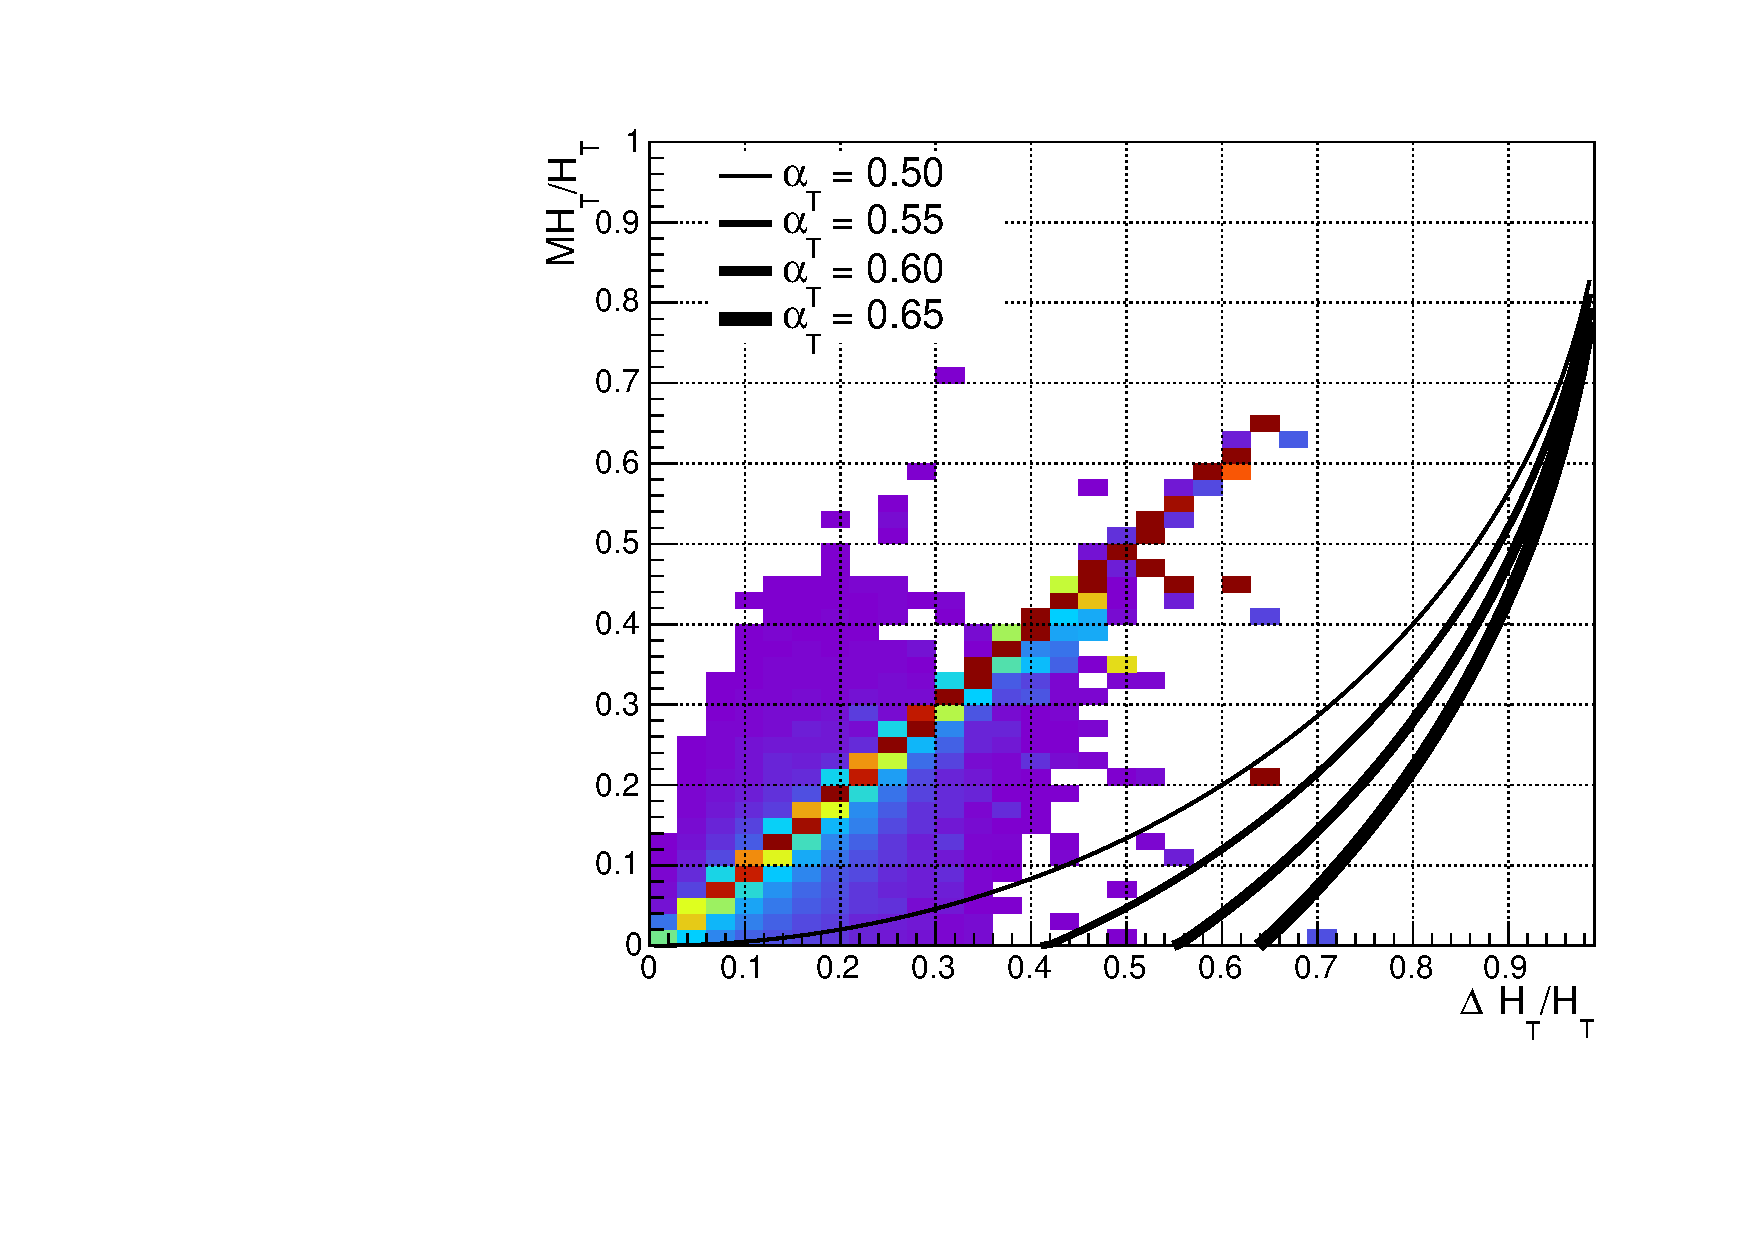
\includegraphics[width=\textwidth]{Figs/alphat/alphat_correlation_QCD.pdf}
    \caption{QCD}
    \label{fig:alphat_corr_qcd}
  \end{subfigure}
  \begin{subfigure}[b]{.46\textwidth}
    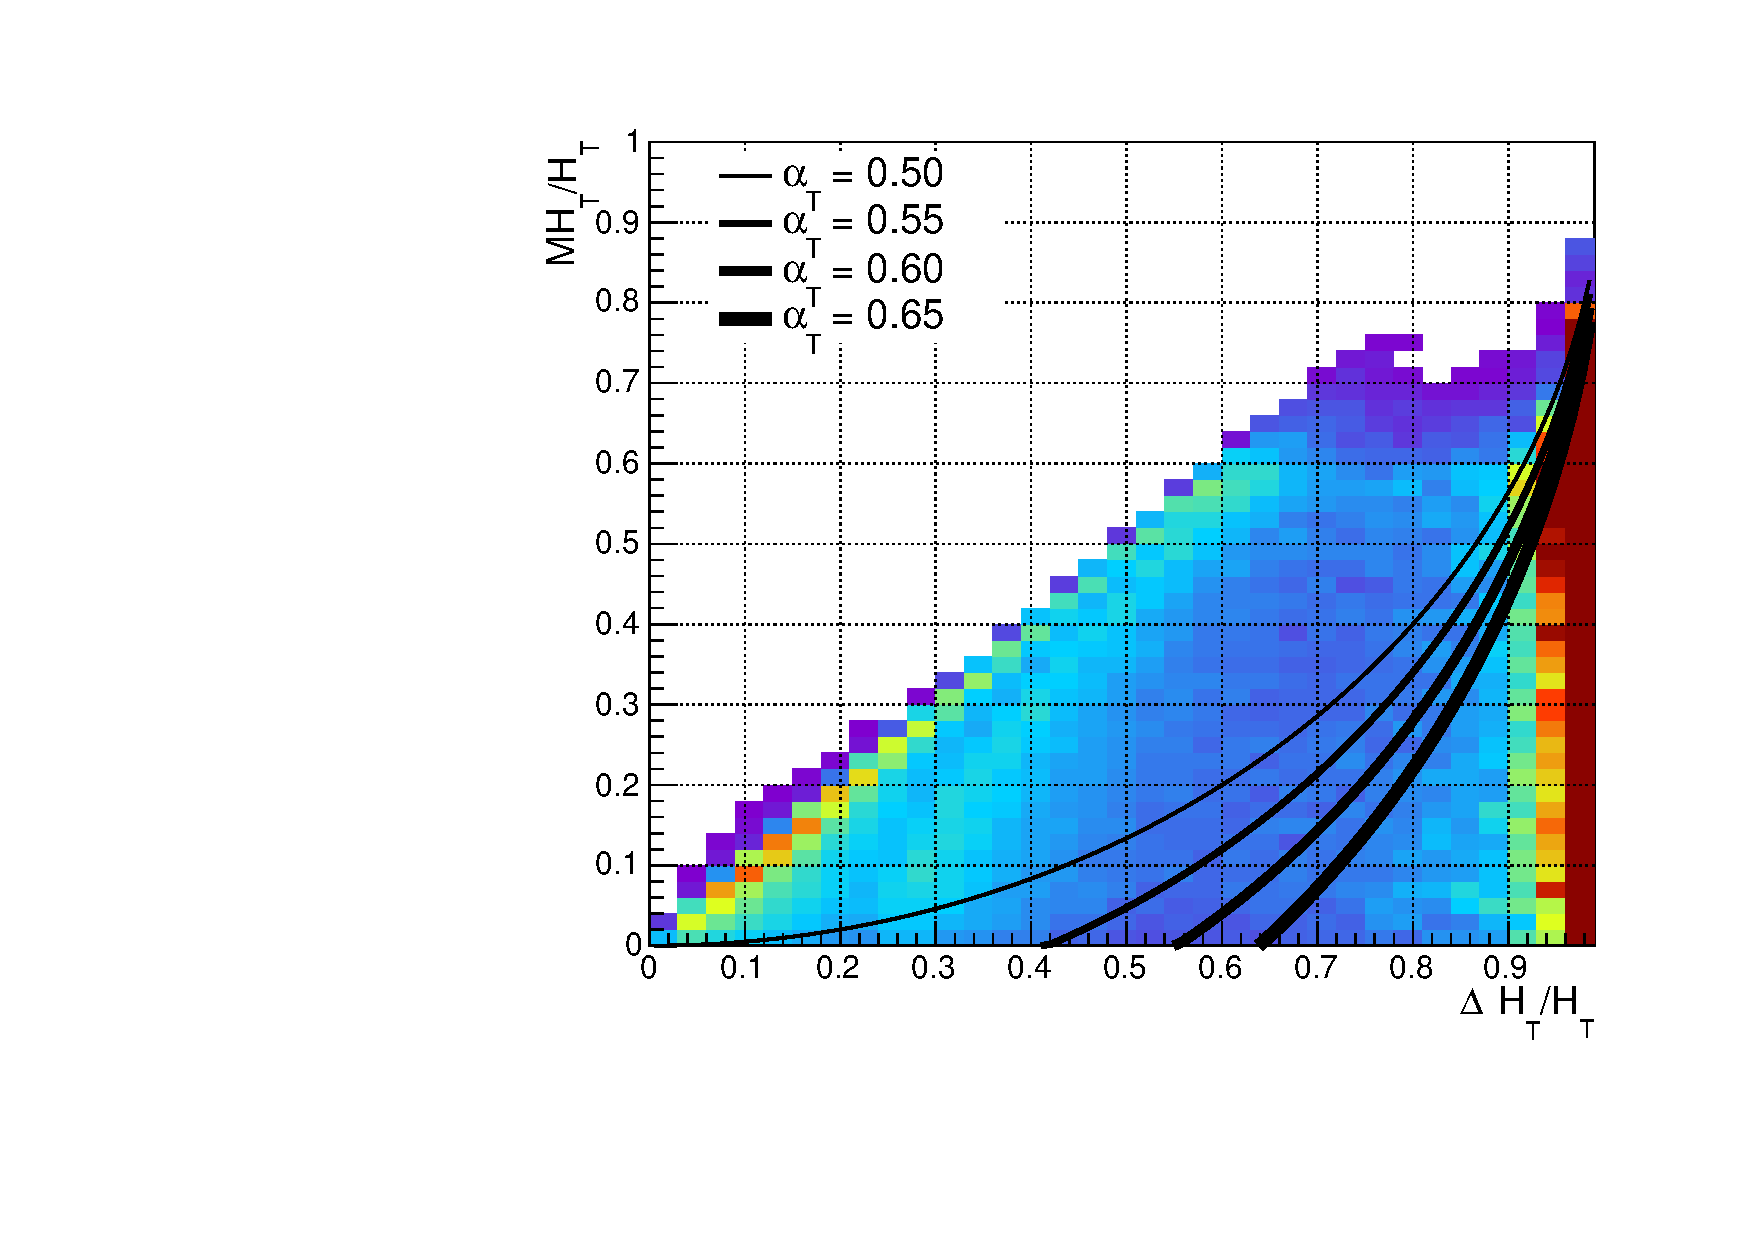
\includegraphics[width=\textwidth]{Figs/alphat/alphat_correlation_Zinv.pdf}
    \caption{\zinv}
    \label{fig:alphat_corr_zinv}
  \end{subfigure}\\
  \begin{subfigure}[b]{.46\textwidth}
    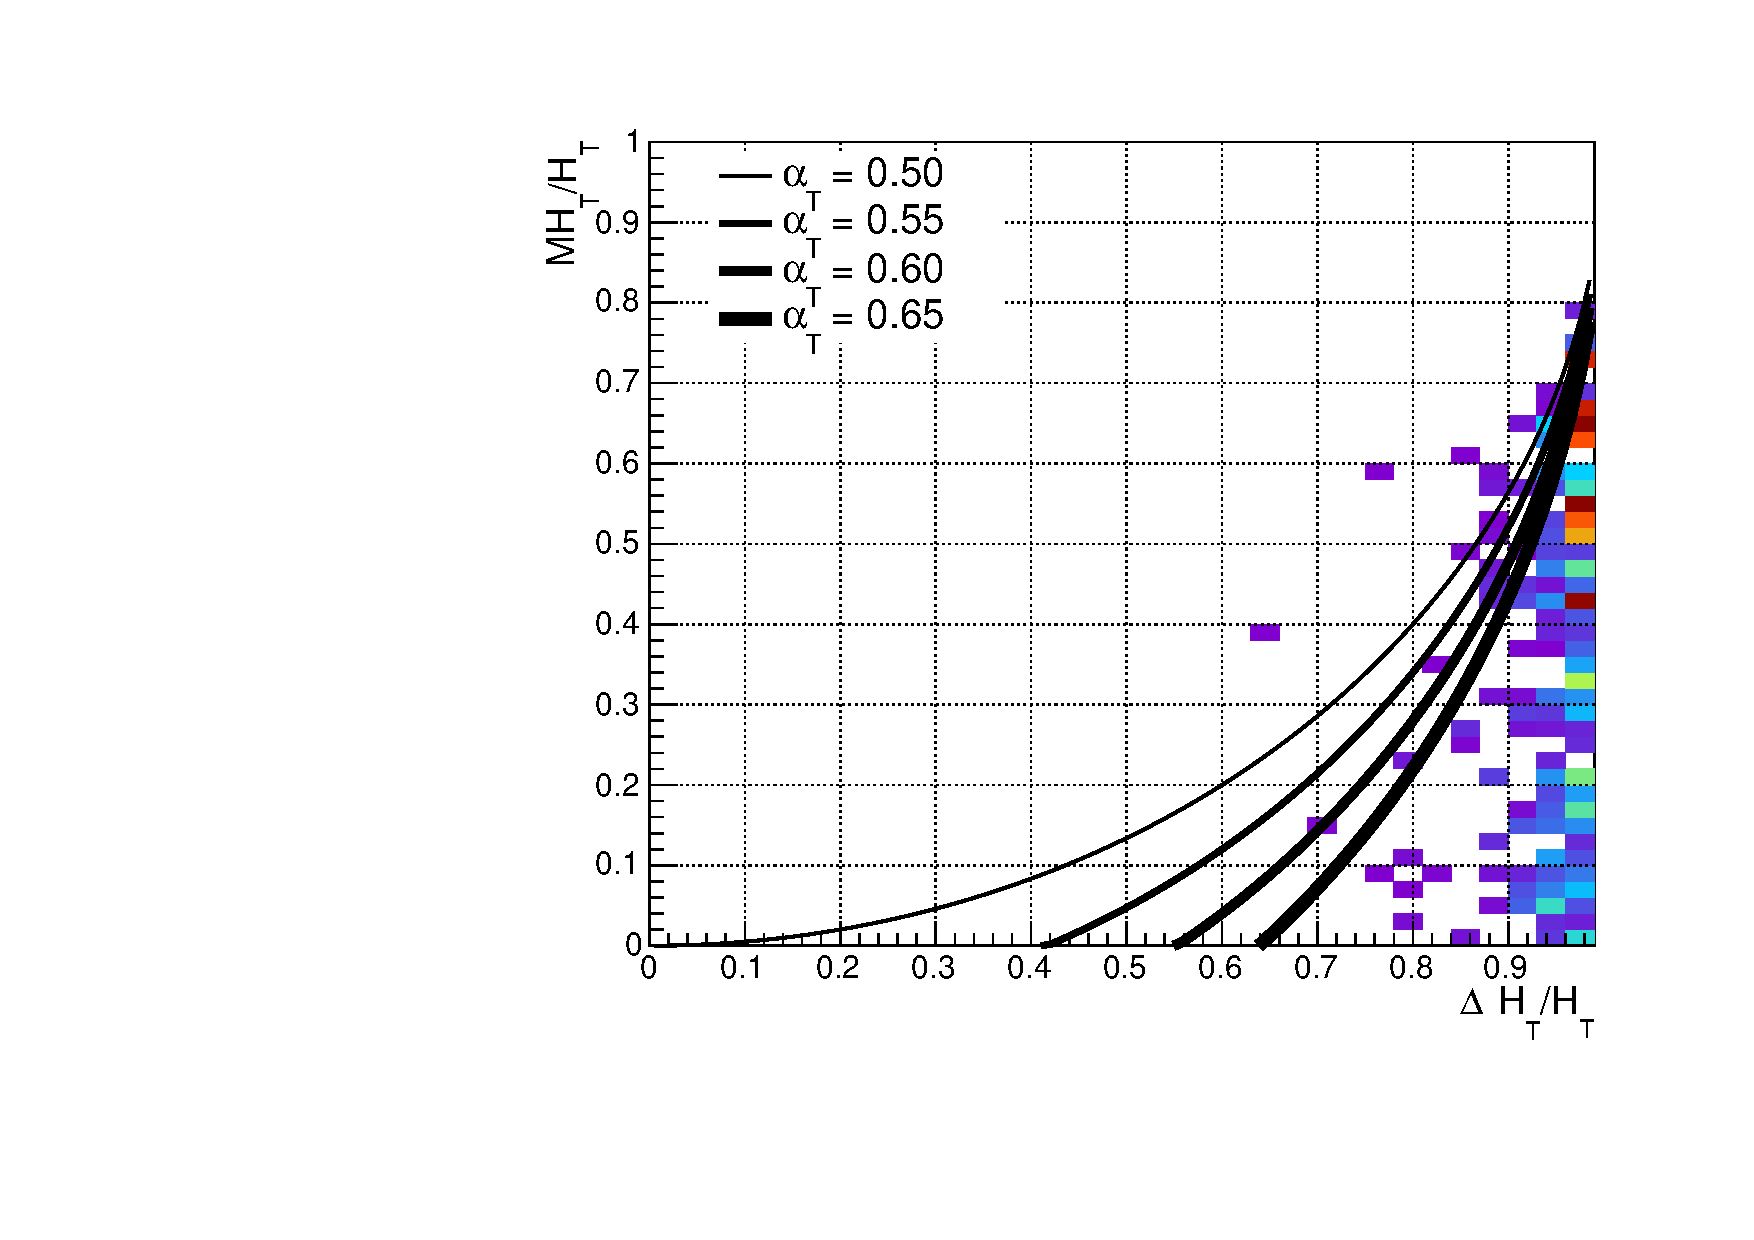
\includegraphics[width=\textwidth]{Figs/alphat/alphat_correlation_T2cc_250_240.pdf}
    \caption{\texttt{T2cc} (250, 240)}
    \label{fig:alphat_corr_t2cc}
  \end{subfigure}
  \caption{Plots showing the correlation between \mht and \deltaHT for QCD,
  \zinv and an example SUSY signature \texttt{T2cc} ($m_{\sTop} = 250$ \gev,
  $m_{\chiz} = 240$ \gev). Contours of constant \alphat are shown in black.
  Each axis is normalised according to the event \HT \emph{show all three?}.}
  \label{fig:alphat_corr}
\end{figure}

Through the requirement of \alphat in a given region of \HT, an implied missing
energy threshold is made. Figure~\ref{fig:alphat_mht_corr} shows this, for the
assumption of \deltaHT = 0 - an assumption which yields the minimal \mht values.
By lowering the \alphat threshold at higher \HT, the implicit missing energy
threshold can be maintained similar to that at low \HT.

\begin{figure}
  \centering
  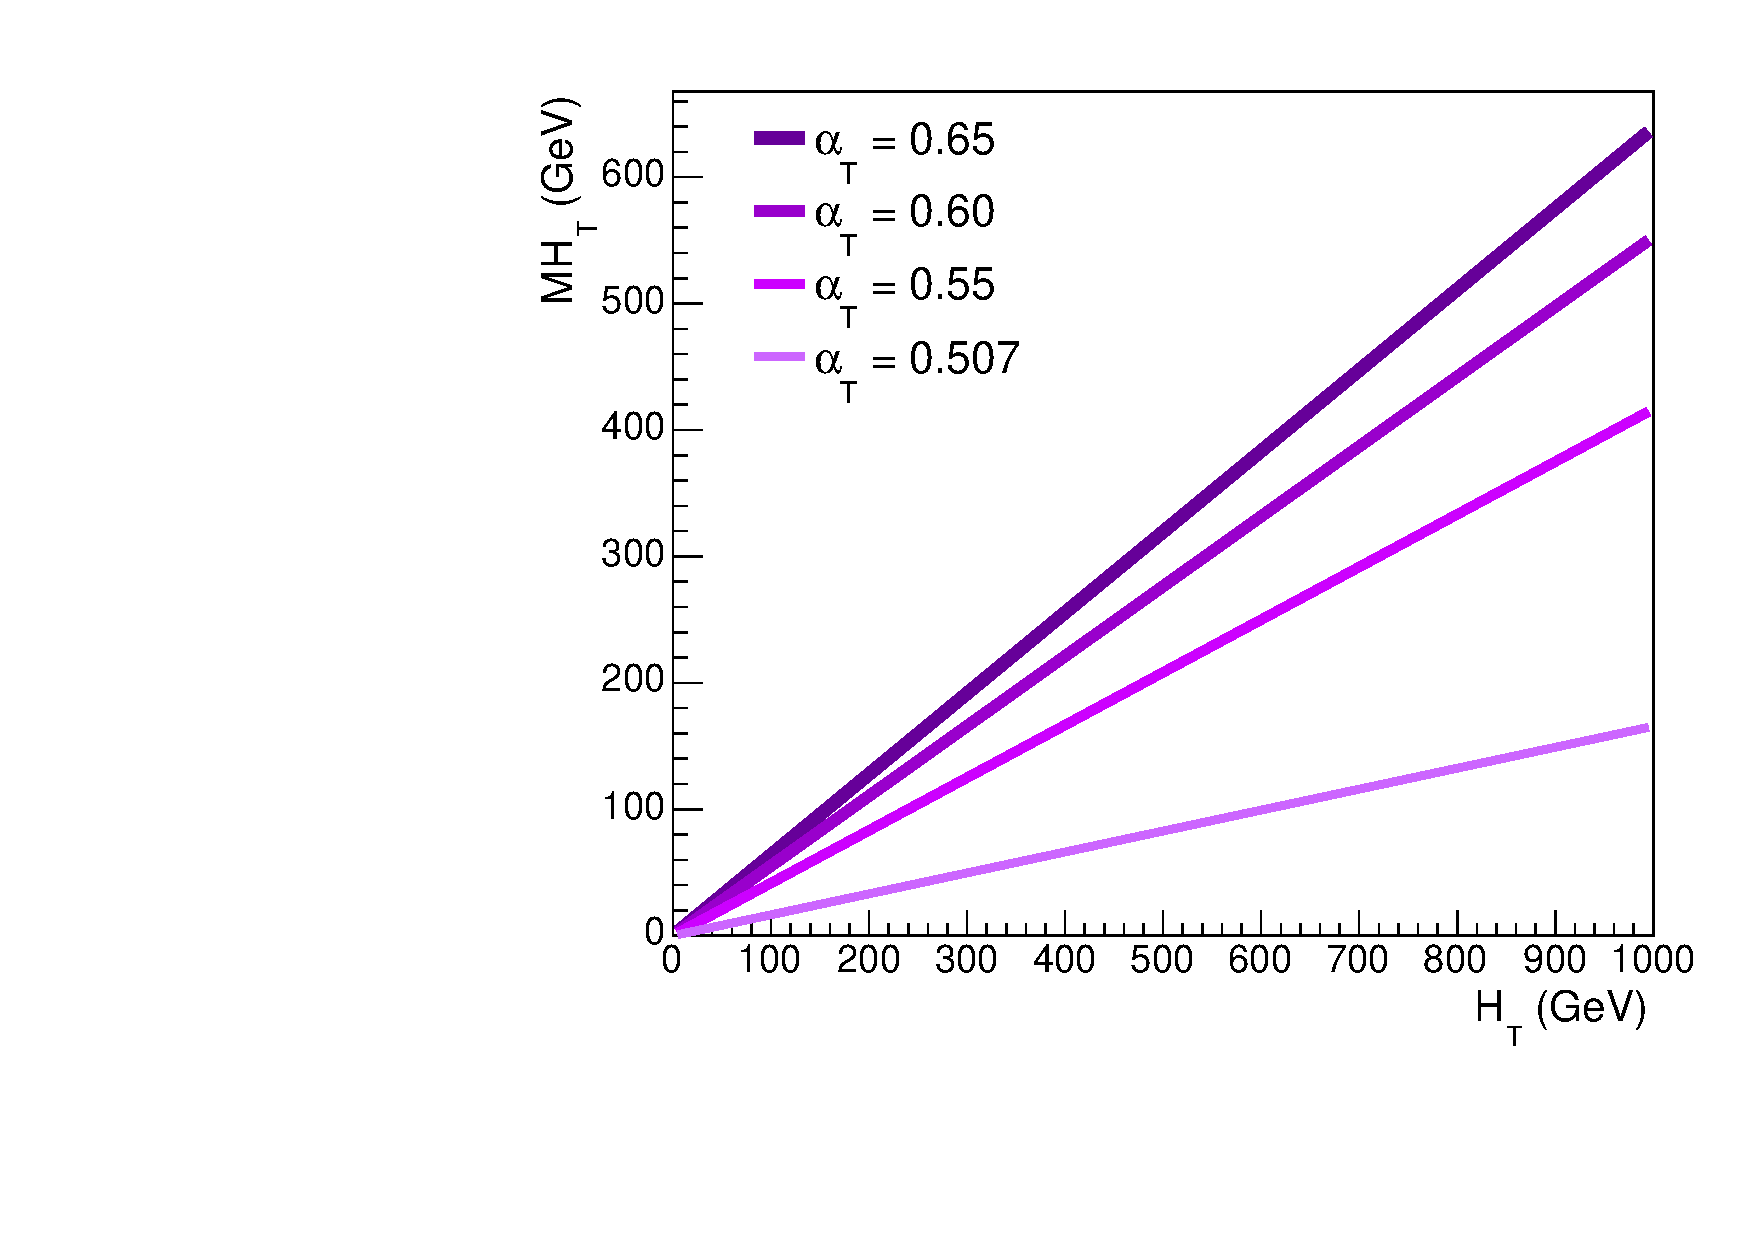
\includegraphics[width=0.7\textwidth]{Figs/alphat/mht_correlation.pdf}
  \caption{The correlation between \HT and \mht for different \alphat values,
  with the assumption of \deltaHT = 0.}
  \label{fig:alphat_mht_corr}
\end{figure}

%********************************** % First Section  *************************************

\section{Standard Model Backgrounds}
\subsection{Genuine \met}
The dominant EWK source of genuine missing energy comes from Z-boson 
production where the Z decays
to neutrinos, \zinv, with associated jet production. This source of background
is considered irreducible.

Events containing leptonic decays of W bosons, \wlnu, originating either
from direct W production, or via the decay of a top quark from \ttbar 
production, are sources of genuine 
missing energy, due to the presence of a weakly interacting neutrino which
evades detection. Such events are vetoed in the signal
region due to the presence of a 
lepton, however if the lepton is missed for whatever reason, leptonic W decays 
can pass the signal selection, forming a significant SM background.

% While lepton and photon vetoes employed in the signal region suppress 
% significant amounts of background from events with neutrinos, such events can 
% still persist if, for example, the lepton is not identified.
% Such processes are predominantly from \ttbar or W-boson production, where the 
% W decays via \wlnu. If the lepton is `lost' and evades our 
% lepton vetoes, significant missing energy can be produced not only from missing 
% the lepton, but from the presence of the neutrino. When such processes are accompanied 
% by associated jet production they are then able to pass our signal region selection.

Leptons can be `lost' for a variety different reasons, but ultimately for failing
the lepton ID criteria. There are numerous potential causes, the 
most prevalent being soft-leptons below ID threshold or non-isolated leptons 
which pass the ID quality cuts but fail the isolation requirement.


% \emph{move to selection section}
% Events containing a Single Isolated Track (SIT) are vetoed from the signal 
% region. This tracker based veto is particularly useful for vetoing additional events 
% that contain leptons which have failed our lepton ID requirements entirely, and 
% are therefore not considered by the leptonic vetoes. Additionally, the veto also
% removes background contributions from single-pronged hadronical decays of $\tau$
% leptons.

While originally designed to target hadronically decaying tau leptons, 
this requirement reduces the remaining lost-lepton backgrounds also.

Following the hadronic selection requirements,
any remaining contributions from SM EWK backgrounds are estimated using a 
fully data-driven transfer factor technique, described in detail in
Section~\ref{sec:background_overview}. A breakdown of the EWK background 
composition is shown in Figure~\ref{fig:background_decomp}, split into the main 
categories of \zinv, \wj, \ttbar and remaining residual backgrounds, such as
single top quark, diboson and Drell-Yann processes.

\begin{figure}[hb!]
\centering
\hspace{0cm}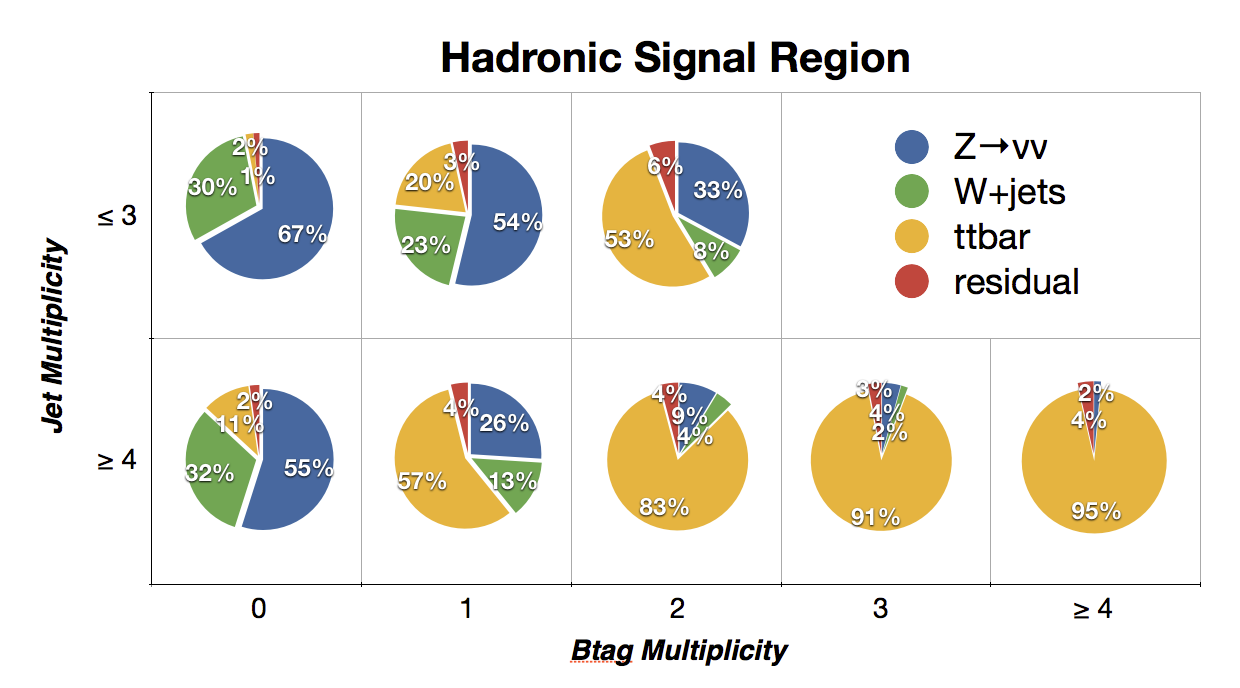
\includegraphics[width=0.9\textwidth, trim=0 00 0 0, clip=true]
{Figs/ra1_had_bg_comp_v3.png}
\caption{The breakdown of the total electroweak background into component
processes as a function of \nj and \nb, for \HT>200 \gev.}
\label{fig:background_decomp}
\end{figure}

\subsection{Fake \met}

As mentioned previously, the dominant source of background for analyses 
searching for a multijet final state is from QCD. A fully-measured QCD event 
would consist of multiple jets balancing each other in all planes, however in 
order to enter the signal region, an event must contain missing energy, 
\mht (equivalent to \met in all-hadronic events).

The most common way for a balanced multijet (MJ) event to gain \mht is when one 
or more of the jets are mis-measured, such that their vectorial sum then leads to non-zero
\mht. This can occur due to detector issues, or due to stochastic fluctuations
within
the inherant jet-resolution of the 
detector. The former is protected against by the \met filters summarised in 
table~\ref{tab:met_filters} and using a filter to remove events
affected by non-functioning or damaged regions of the ECAL system, where 
events are vetoed if they contain significant energy deposits within a given 
distance from a known problematic region. The latter is dealt with using a
cut on the \alphat variable where 
events with fake missing energy signatures give values $<0.5$.

QCD MJ events can also appear to contain non-zero missing energy 
due to the threshold requirements of jets. If an event contains 
one or more jets below the analysis threshold, then the 
event is measured as imbalanced and containing \mht. Events such as these are largely 
removed with the \alphat requirement, however in addition a requirement is made on the
ratio \mhtmet.

% Finally, it is also possible for rare instrumentation effects to lead to jet 
% energy
% mismeasurements. To protect against this, a suite of MET filters are defined by 
% the JetMET \emph{POG}, and are applied to all selections.


\section{Signal Triggers}

Events are collected at the HLT using a dedicated suite of
signal triggers. For an event to pass the trigger
requirements, it must exceed both a \HT and an \alphat threshold. Trigger rate 
can be maintained by varying the
threshold requirement on each of these independent requirements, as shown in
Table~\ref{tab:sig_trigs}. Each \HT bin in the analysis is seeded by a
particular signal
trigger, with a 25 \gev offset in online and offline \HT, with the exception of
the 200 \gev bin.

Exclusively for this analysis, the additional `Parked' trigger 
\\\verb!HT200_AlphaT0p57! is included, seeding the new \HT> 200 \gev bin. Such a low
threshold allow sensitivity to be maintained for softer physics signatures, such
as those expected from compressed spectra SUSY decays.

\begin{table}[!ht]
  \caption{Signal triggers, the L1 seed triggers and their efficiencies measured
  for per \HT and \nj category.}
  \label{tab:sig_trigs}
  \centering
  \scriptsize
  \begin{tabular}{ cccccc }
    \hline
    \hline
    Offline \HT       & Offline \alphat & L1 seed (\verb!L1_?!)         & Trigger (\verb!HLT_?!)  & \multicolumn{2}{c}{Efficiency (\%)}          \\ [0.5ex]
    region (\gev)         & threshold       & (highest thresholds)          &                         & $2 \leq \nj \leq 3$ & $\nj \geq 4$       \\ [0.5ex]
    \hline
    $200 < \HT < 275$ & 0.65            & \verb!DoubleJetC64!           & \verb!HT200_AlphaT0p57! & $81.8^{+0.4}_{-0.4}$  & $78.9^{+0.3}_{-0.4}$ \\
    $275 < \HT < 325$ & 0.60            & \verb!DoubleJetC64!           & \verb!HT200_AlphaT0p57! & $95.2^{+0.3}_{-0.4}$  & $90.0^{+1.2}_{-1.3}$ \\
    $325 < \HT < 375$ & 0.55            & \verb!DoubleJetC64 OR HTT175! & \verb!HT300_AlphaT0p53! & $97.9^{+0.3}_{-0.3}$  & $95.6^{+0.9}_{-1.0}$ \\
    $375 < \HT < 475$ & 0.55            & \verb!DoubleJetC64 OR HTT175! & \verb!HT350_AlphaT0p52! & $99.2^{+0.2}_{-0.2}$  & $98.7^{+0.5}_{-0.7}$ \\
    $\HT > 475$       & 0.55            & \verb!DoubleJetC64 OR HTT175! & \verb!HT400_AlphaT0p51! & $99.8^{+0.1}_{-0.3}$  & $99.6^{+0.3}_{-0.7}$ \\
    \hline
    \hline
  \end{tabular}
\end{table}

Trigger efficiencies are measured using an unbiased single muon reference
trigger,
\\\verb!HLT_IsoMu24_eta2p1!, using a muon tag and probe method where a
single muon is selected and then subsequently ignored from the analysis when 
calculating event level variables such as \HT, \mht and \alphat. Efficiencies 
are measured for each \HT bin and for each \nj category, as summarised in 
table~\ref{tab:sig_trigs}. Example trigger `turn-on' curves are shown for the 3 
lowest \HT bins in figures~\ref{fig:eff_alphat_le3j} and \ref{fig:eff_alphat_ge4j}.
The curves are shown both differentially and cumulatively, to show the
efficiency for events of a given \alphat value and above an \alphat threshold
respectively.
Across the higher \HT 
bins the triggers are fully efficient. Inefficiencies in the low \HT bins are
understood as being due to the relatively high threshold L1 seed trigger used
for this region, in order to maintain
low rates in the high PU environment encountered throughout \runone. Lower 
efficiencies are also observed in the \njhigh category attributed to the presence of 
softer jets, as an increased number of jets must equate to the same total \HT 
requirement of the bin.

\afterpage{%
\begin{figure}[!ht]
  \centering
    \begin{subfigure}[b]{0.48\textwidth}
      
\includegraphics[width=\textwidth,page=11, trim=0 0 0 20, clip=true]{figures/trigger/HT200_275_73_73_36_AlphaT_le3j_RunAtFNAL}
      \caption{Differential, $200 < \HT < 275 $ \gev}
    \end{subfigure}
    \begin{subfigure}[b]{0.48\textwidth}
      
\includegraphics[width=\textwidth,page=18, trim=0 0 0 20, clip=true]{figures/trigger/HT200_275_73_73_36_AlphaT_le3j_RunAtFNAL}
      \caption{Cumulative, $200 < \HT < 275 $ \gev}
    \end{subfigure} \\
    \vspace{0.5cm}\begin{subfigure}[b]{0.48\textwidth}
      
\includegraphics[width=\textwidth,page=11, trim=0 0 0 20, clip=true]{figures/trigger/HT275_325_73_73_36_AlphaT_le3j_RunAtFNAL}
      \caption{Differential, $275 < \HT < 325 $ \gev}
    \end{subfigure}
    \begin{subfigure}[b]{0.48\textwidth}
      
\includegraphics[width=\textwidth,page=18, trim=0 0 0 20, clip=true]{figures/trigger/HT275_325_73_73_36_AlphaT_le3j_RunAtFNAL}
      \caption{Cumulative, $275 < \HT < 325 $ \gev}
    \end{subfigure} \\
    \vspace{0.5cm}\begin{subfigure}[b]{0.48\textwidth}
      
\includegraphics[width=\textwidth,page=11, trim=0 0 0 20, clip=true]{figures/trigger/HT325_375_86_86_43_AlphaT_le3j_RunAtFNAL}
      \caption{Differential, $325 < \HT < 375 $ \gev}
    \end{subfigure}
    \begin{subfigure}[b]{0.48\textwidth}
      
\includegraphics[width=\textwidth,page=18, trim=0 0 0 20, clip=true]{figures/trigger/HT325_375_86_86_43_AlphaT_le3j_RunAtFNAL}
      \caption{Cumulative, $325 < \HT < 375 $ \gev}
    \end{subfigure} \\
  
    \caption{\label{fig:eff_alphat_le3j}
      Differential (left) and Cumulative (right) efficiency turn-on curves for 
      the signal triggers, for the three lowest \HT bins and \njlow.}
\end{figure}
\clearpage
}

\afterpage{%
\begin{figure}[!ht]
  \centering
    \begin{subfigure}[b]{0.48\textwidth}
      
\includegraphics[width=\textwidth,page=11]{figures/trigger/HT200_275_73_73_36_AlphaT_ge4j_RunAtFNAL}
      \caption{Differential, $200 < \HT < 275 $ \gev}
    \end{subfigure}
    \begin{subfigure}[b]{0.48\textwidth}
      
\includegraphics[width=\textwidth,page=18]{figures/trigger/HT200_275_73_73_36_AlphaT_ge4j_RunAtFNAL}
      \caption{Cumulative, $200 < \HT < 275 $ \gev}
    \end{subfigure} \\
    \begin{subfigure}[b]{0.48\textwidth}
      
\includegraphics[width=\textwidth,page=11]{figures/trigger/HT275_325_73_73_36_AlphaT_ge4j_RunAtFNAL}
      \caption{Differential, $275 < \HT < 325 $ \gev}
    \end{subfigure}
    \begin{subfigure}[b]{0.48\textwidth}
      
\includegraphics[width=\textwidth,page=18]{figures/trigger/HT275_325_73_73_36_AlphaT_ge4j_RunAtFNAL}
      \caption{Cumulative, $275 < \HT < 325 $ \gev}
    \end{subfigure} \\
    \begin{subfigure}[b]{0.48\textwidth}
      
\includegraphics[width=\textwidth,page=11]{figures/trigger/HT325_375_86_86_43_AlphaT_ge4j_RunAtFNAL}
      \caption{Differential, $325 < \HT < 375 $ \gev}
    \end{subfigure}
    \begin{subfigure}[b]{0.48\textwidth}
      
\includegraphics[width=\textwidth,page=18]{figures/trigger/HT325_375_86_86_43_AlphaT_ge4j_RunAtFNAL}
      \caption{Cumulative, $325 < \HT < 375 $ \gev}
    \end{subfigure} \\
  
    \caption{\label{fig:eff_alphat_ge4j}
      Differential (left) and Cumulative (right) efficiency turn-on curves for 
      the signal triggers, for the three lowest \HT bins and \njhigh.}
\end{figure}
\clearpage
}

All triggers were present throughout \runone, however the 
\\\verb!HLT_HT200_AlphaT0p57! trigger was used as part of the `Parked' stream of 
data which was reconstructed at a later date, following the active data taking 
period. During data taking triggers may have `prescale' factors applied to them 
such that only every $n$ triggered events are actually recorded, however all of
the signal triggers remained unprescaled for the entirety of the 8 \tev
data taking.


\section{Selection Criteria}
\label{sec:selec_crit}

Event selection requirements for the hadronic signal region are chosen with an
aim to
maintain sensitivity to hadronically decaying sparticle production, while 
rejecting as many QCD-type processes as possible. To do so, requirements are 
made on:

\begin{description}
\item[Jets]
Events are required to contain at least two jets with at least
$\HT > 200$ \gev, to ensure the presence of significant hadronic activity. As 
mentioned previously, events are categorised by \HT, with jet \Pt
requirements on the two leading and the remaining additional jets seperately.
The jet \Pt thresholds vary as a function of the \HT bin of the event, as shown in
Table~\ref{tab:jet_pt_thresholds}, in order to maintain a similar kinematic
phase space throughout the \HT range.

\begin{table}[h!]
  \caption{Jet \Et thresholds per \HT bin.\label{tab:jet_pt_thresholds}}
  \centering
  \footnotesize
  \begin{tabular}{ lcccc }
    \hline
    \hline
    \HT bin        & 200--275 & 275--325 & 325--375 & $>$375 \\
    \hline
    Lead jet       & 73.3     & 73.3     & 86.7     & 100.0  \\
    Second jet     & 73.3     & 73.3     & 86.7     & 100.0  \\
    All other jets & 36.7     & 36.7     & 43.3     & 50.0   \\
    \hline
    \hline
  \end{tabular}
\end{table}

\item[Leptons]
Any events containing leptons are vetoed to ensure hadronic events
are considered, thereby suppressing events with genuine \met from leptonic decays to
neutrinos such as \wlnu.

\item[Photons]
Events containing photons are vetoed, for similar reasons as the leptonic 
vetoes, in order to maintain a purely hadronic environment.

\item[Single Isolated Tracks]
Events containing a Single Isolated Track (SIT) are vetoed from the signal 
region. This tracker based veto is particularly useful for vetoing additional events 
that contain leptons which have failed our lepton ID requirements entirely, and 
are therefore not considered by the leptonic vetoes. Additionally, the veto also
removes background contributions from single-pronged hadronical decays of $\tau$
leptons.

\item[Event]
The topology of the event is required to pass a threshold of $\alphat > 0.55$, 
a requirement which itself varies as a function of the \HT category being
considered, always
chosen such that the signal triggers are in the efficiency plateau. While no
absolute \met requirement is made, the cut on
\alphat imposes an implied threshold, which maintains the analysis'
sensitivity to very low regions of \met as shown by figure~\ref{fig:alphat_mht_corr}.

\end{description}

\section{Residual QCD cleaning}

While the \alphat requirement removes many order of magnitude of QCD events,
there still exists scenarios in which events may pass the signal region
selection. Accordingly, further requirements are made to ensure the search
region is free of any residual QCD contamination.

\subsection{Multiple jets below threshold}
\label{sec:qcd_cleaning_below_thresh}

\begin{figure}[ht!]
\centering
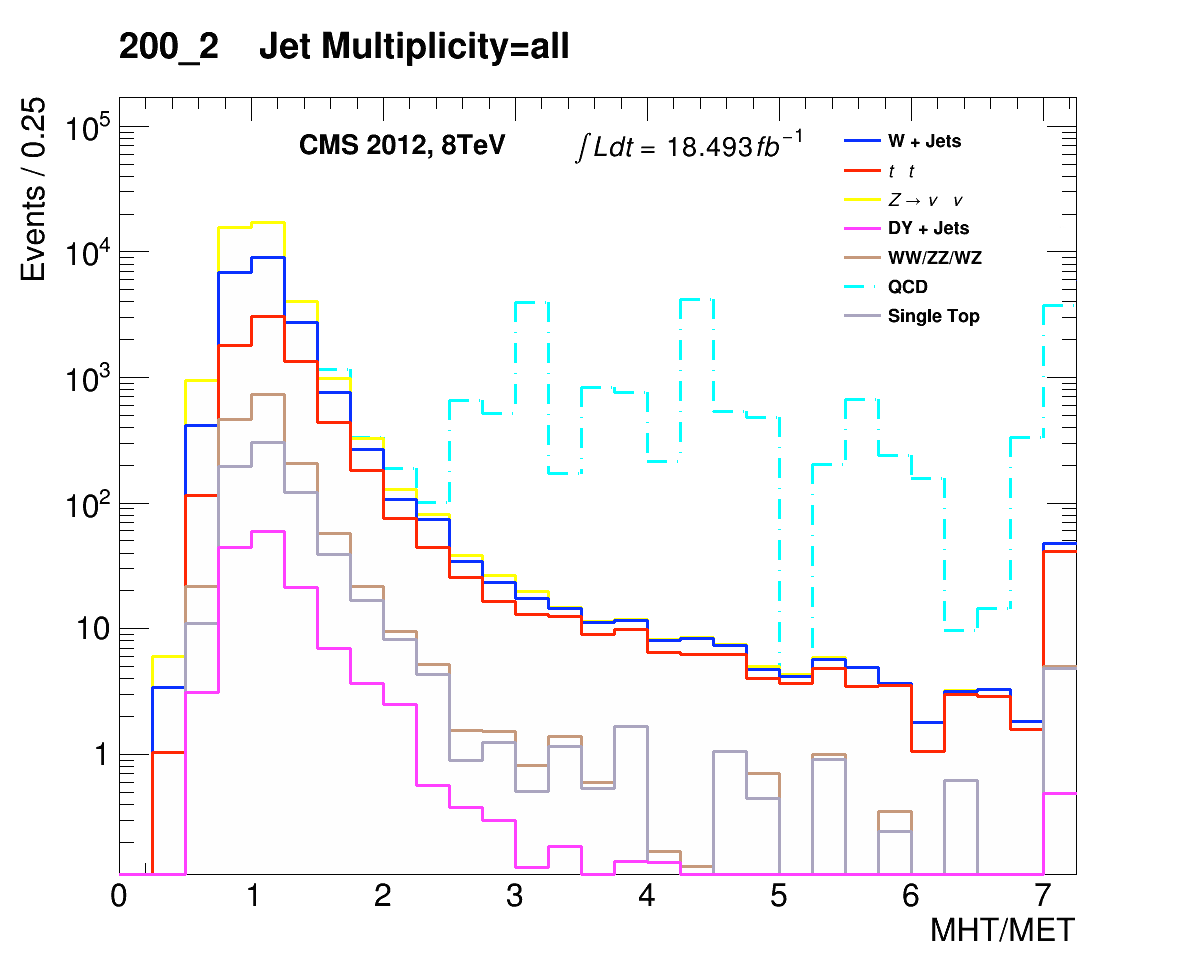
\includegraphics[width=0.6\textwidth]
{Figs/datamc/had/v1/Stacked_MHTovMET_all_200_upwards.png}
\caption{The \mhtmet distribution of MC events following the hadronic selection
criteria, minus the \mhtmet requirement.The MC yields are stacked,
with the QCD contribution shown in cyan. The plot is for a fully inclusive
selection of $\nb \geq 0$, $\nj \geq 2$ and \HT > 200 \gev.}
\label{fig:full_mhtmet_distro}
\end{figure}

Events can acquire non-negligible amounts of \mht without the presence of
real \met if multiple jets are below the analysis threshold, where their
configuration can conspire to give a topology passing the \alphat thresholds.
Such events will contain a disparity between the energy deposit based \met and
jet object based \mht variables. This effect is seen in
figure~\ref{fig:full_mhtmet_distro} where the presence of significant QCD
contamination at high values of \mhtmet is observed, despite an \alphat
requirement. To protect against this scenario, events are required to have a low
ratio of the two variables, specifically \mhtmet < 1.25.


\subsection{Instrumental effects}

Fake \mht may also be produced if jets overlap with areas of the calorimeter 
system which are damaged or known to be faulty, where jets can be mis-measured or 
lost as a result. To protect against this, for a given jet $j$, the angular separation
between the event \mht, calculated excluding jet $j$, and the jet itself is used, defined
as:
% 
\begin{equation}
\dphistar_j = \Delta \phi\big(\overrightarrow{\Pt}_j,-\sum_{i\neq j}
{\overrightarrow{\Pt}_i}\big) .
\label{eq:biasdphi}
\end{equation}
% 
An advantage of this variable with respect to the often used
$\Delta R(jet, MHT)$ is it's detection of spurious missing energy vectors caused
by both under-measurements and over-measurements of a jet's transverse momentum.
A small value of $\dphistar_j$ indicates that the momentum vector of $j$
is aligned with the \mht vector, implying the jet is mis-measured. Events are 
vetoed if a jet with \dphistar< 0.5 is within $\Delta R < 0.3$ of a known
`dead' region of the ECAL.

Multiple event filters are applied to remove any jet mismeasurements arising due
to instrumental effects, however previously un-discovered and
therefore rare detector effects may hypothetically be present. To check
for this, the
jet giving the minimum \dphistar value in an event, \mindphistar, is found,
and a single entry of the $\eta$ and $\phi$ direction of the jet's axis is entered
into a map of the detector, figure~\ref{fig:hotspots}. Any areas of instrumental issue would
be visible as clusters of high event counts. Figures~\ref{fig:hotspots_2d_nodeadECAL} and
\ref{fig:hotspots_1d_nodeadECAL} shows the detector map and the 1d distribution
of counts are shown before the dead ECAL filter is applied. Areas of
potential instrumental defects are clearly visible, notably as outliers in
figure~\ref{fig:hotspots_1d_nodeadECAL}. Following the application of the dead
ECAL filter the hotspot areas and the corresponding outliers removed, as seen in
figures~\ref{fig:hotspots_2d_withdeadECAL} and
\ref{fig:hotspots_1d_withdeadECAL}, indicating there to be no
remaining instrumental issues.

\begin{figure}[h!]
  \begin{center}
    \begin{subfigure}[b]{0.46\textwidth}
      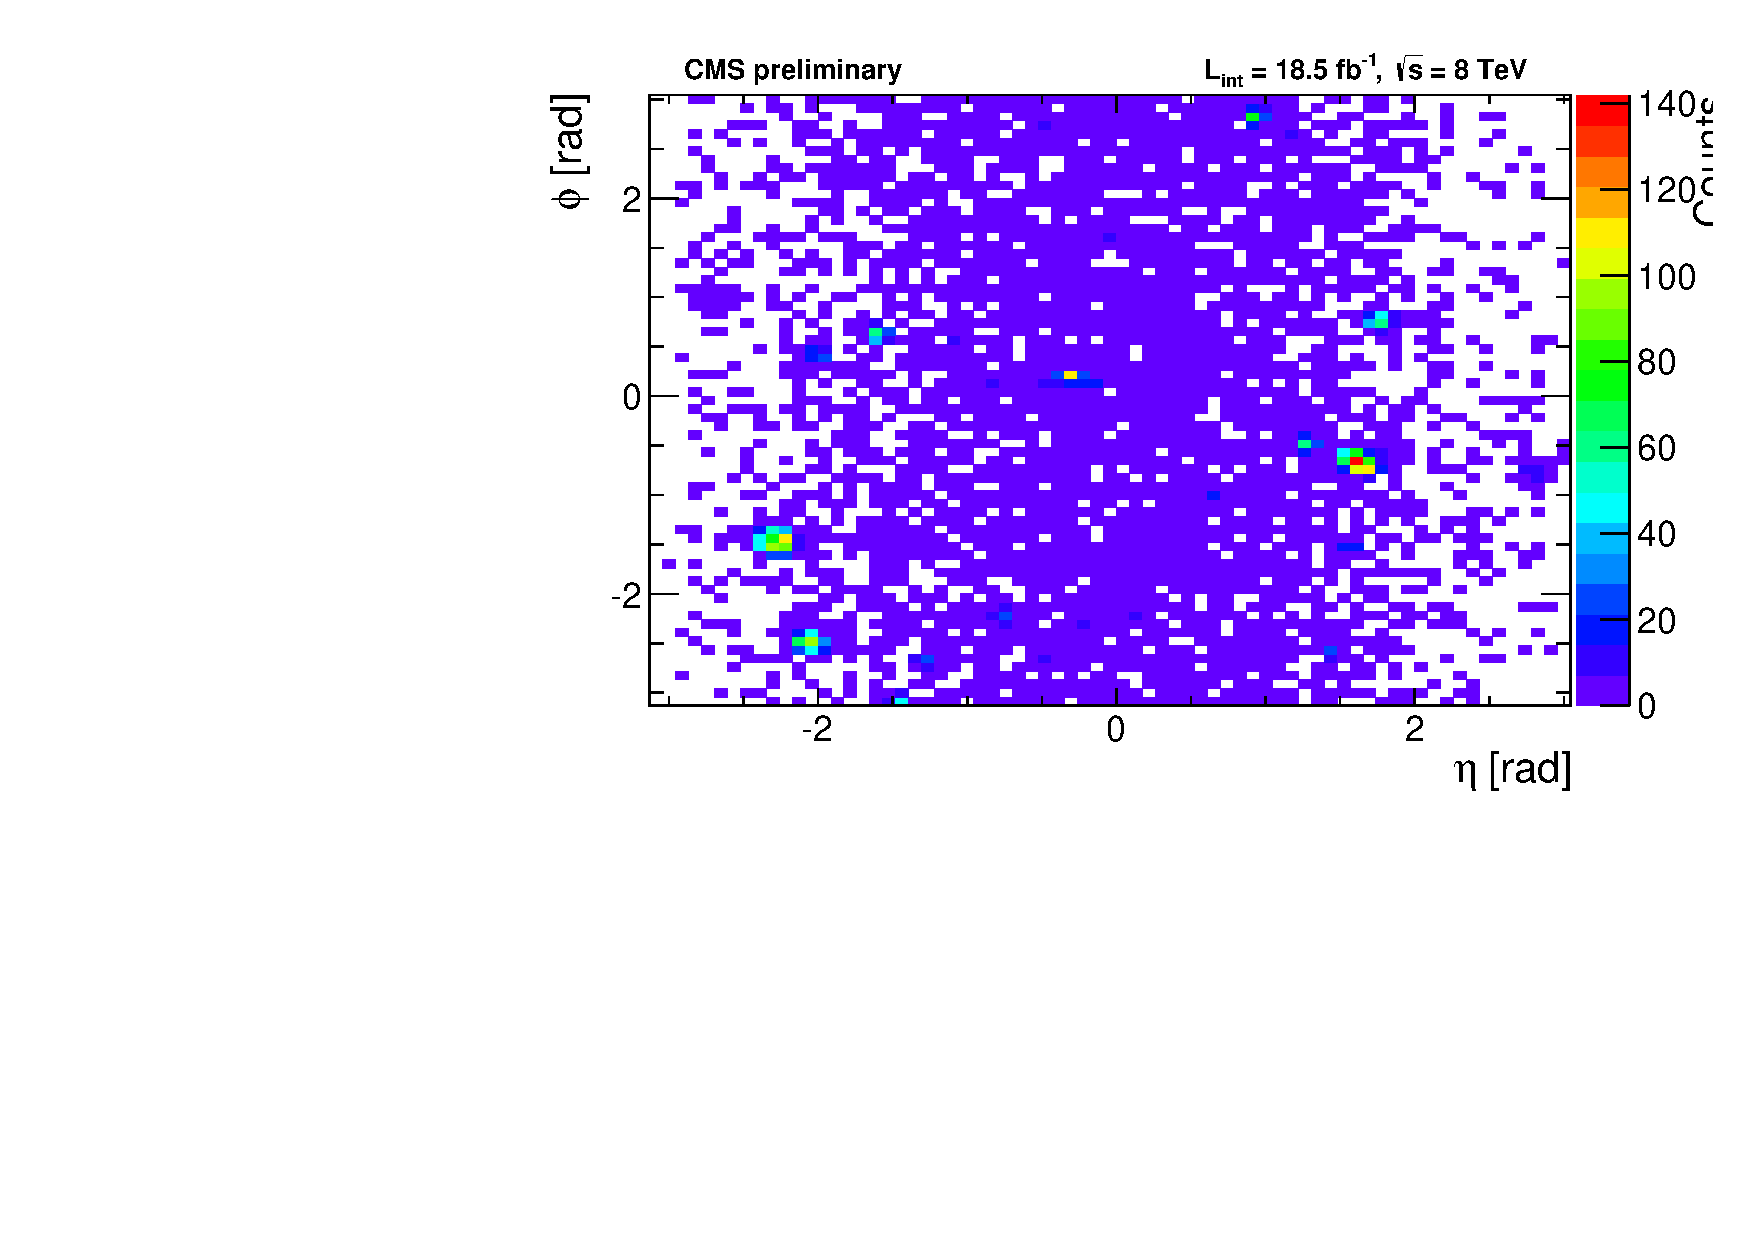
\includegraphics[width=\textwidth]{Figs/dphi/HT_dependent_AlphaT_thresholds/th2d_denom_summed_ge2j_ge0b_200.pdf}
      \caption{No ``dead ECAL filter''.}
      \label{fig:hotspots_2d_nodeadECAL}
    \end{subfigure}
    \begin{subfigure}[b]{0.46\textwidth}
      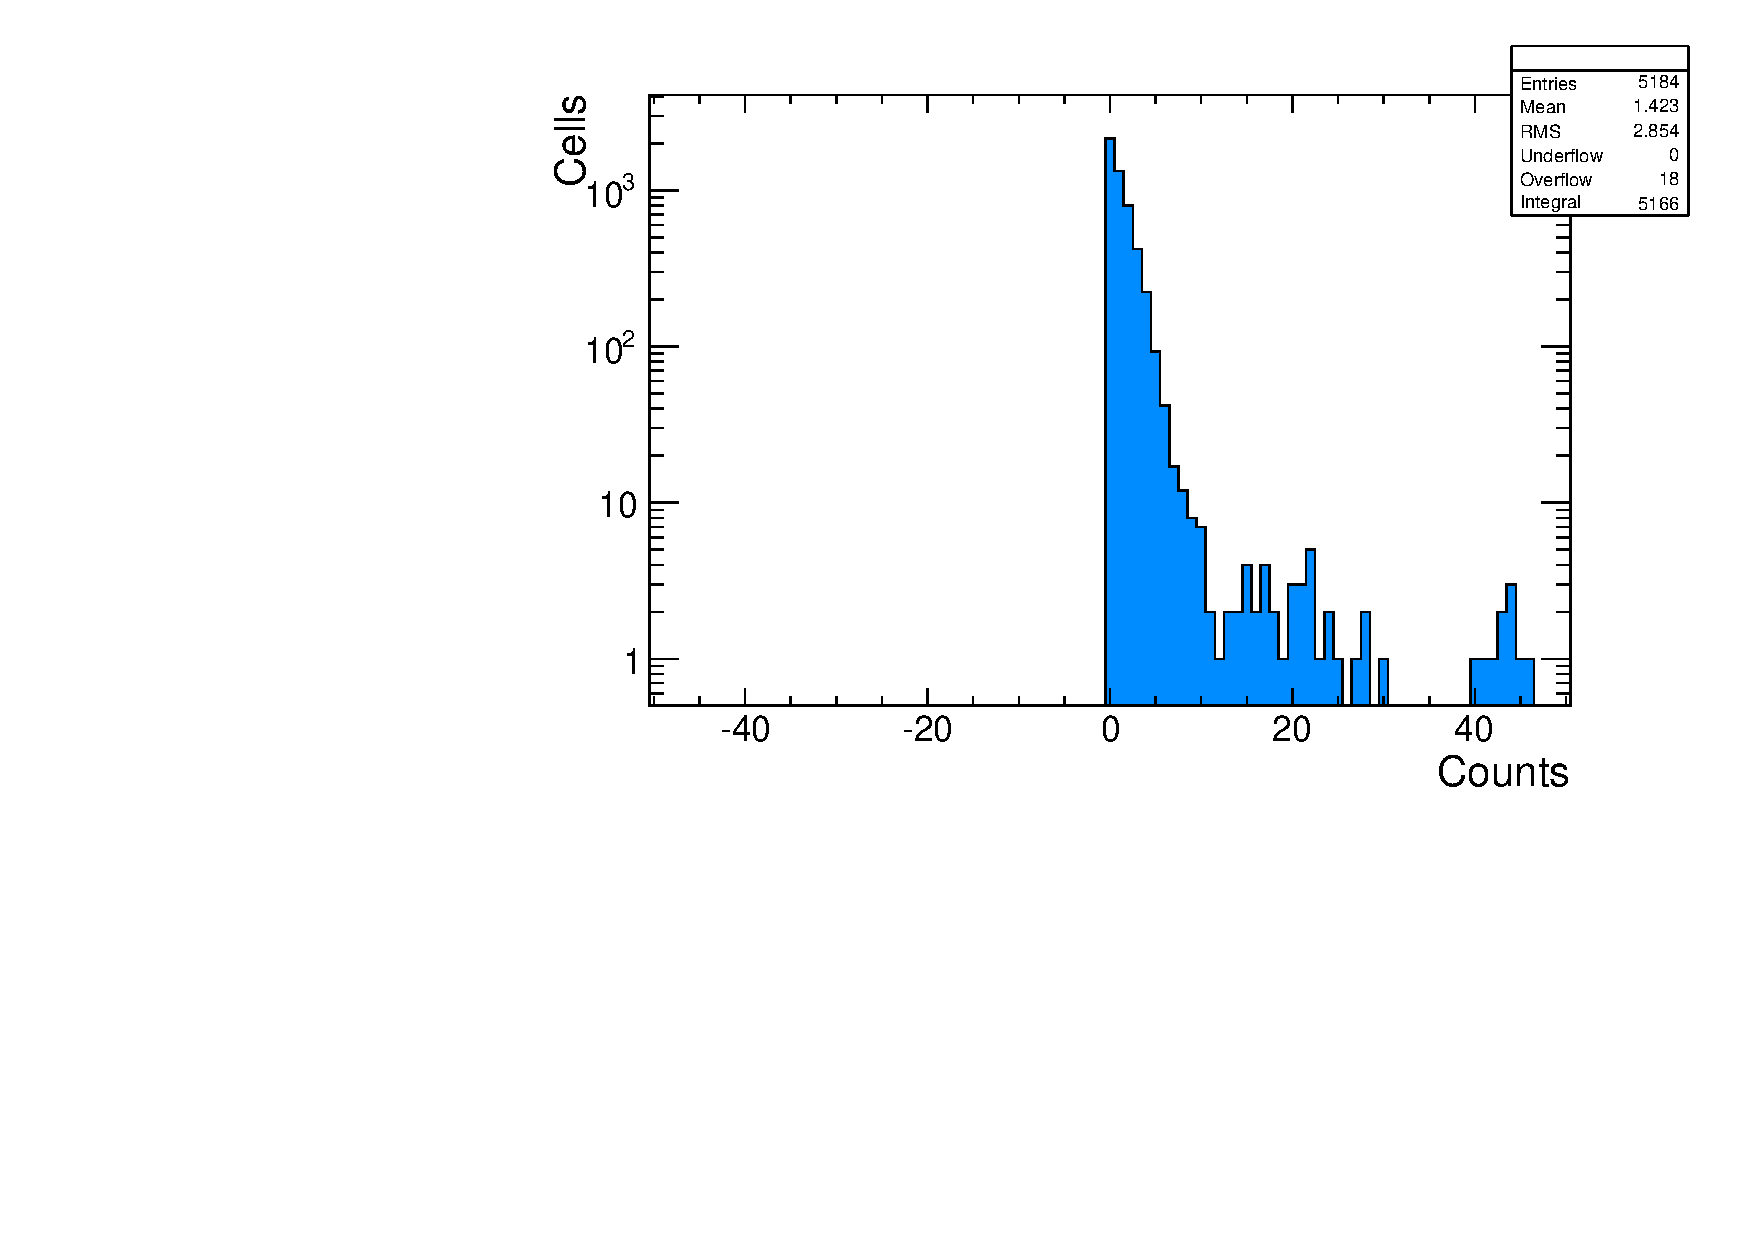
\includegraphics[width=\textwidth]{Figs/dphi/HT_dependent_AlphaT_thresholds/th1d_denom_summed_ge2j_ge0b_200.pdf}
      \caption{No ``dead ECAL filter''.}
      \label{fig:hotspots_1d_nodeadECAL}
    \end{subfigure} \\ 
    \begin{subfigure}[b]{0.46\textwidth}
      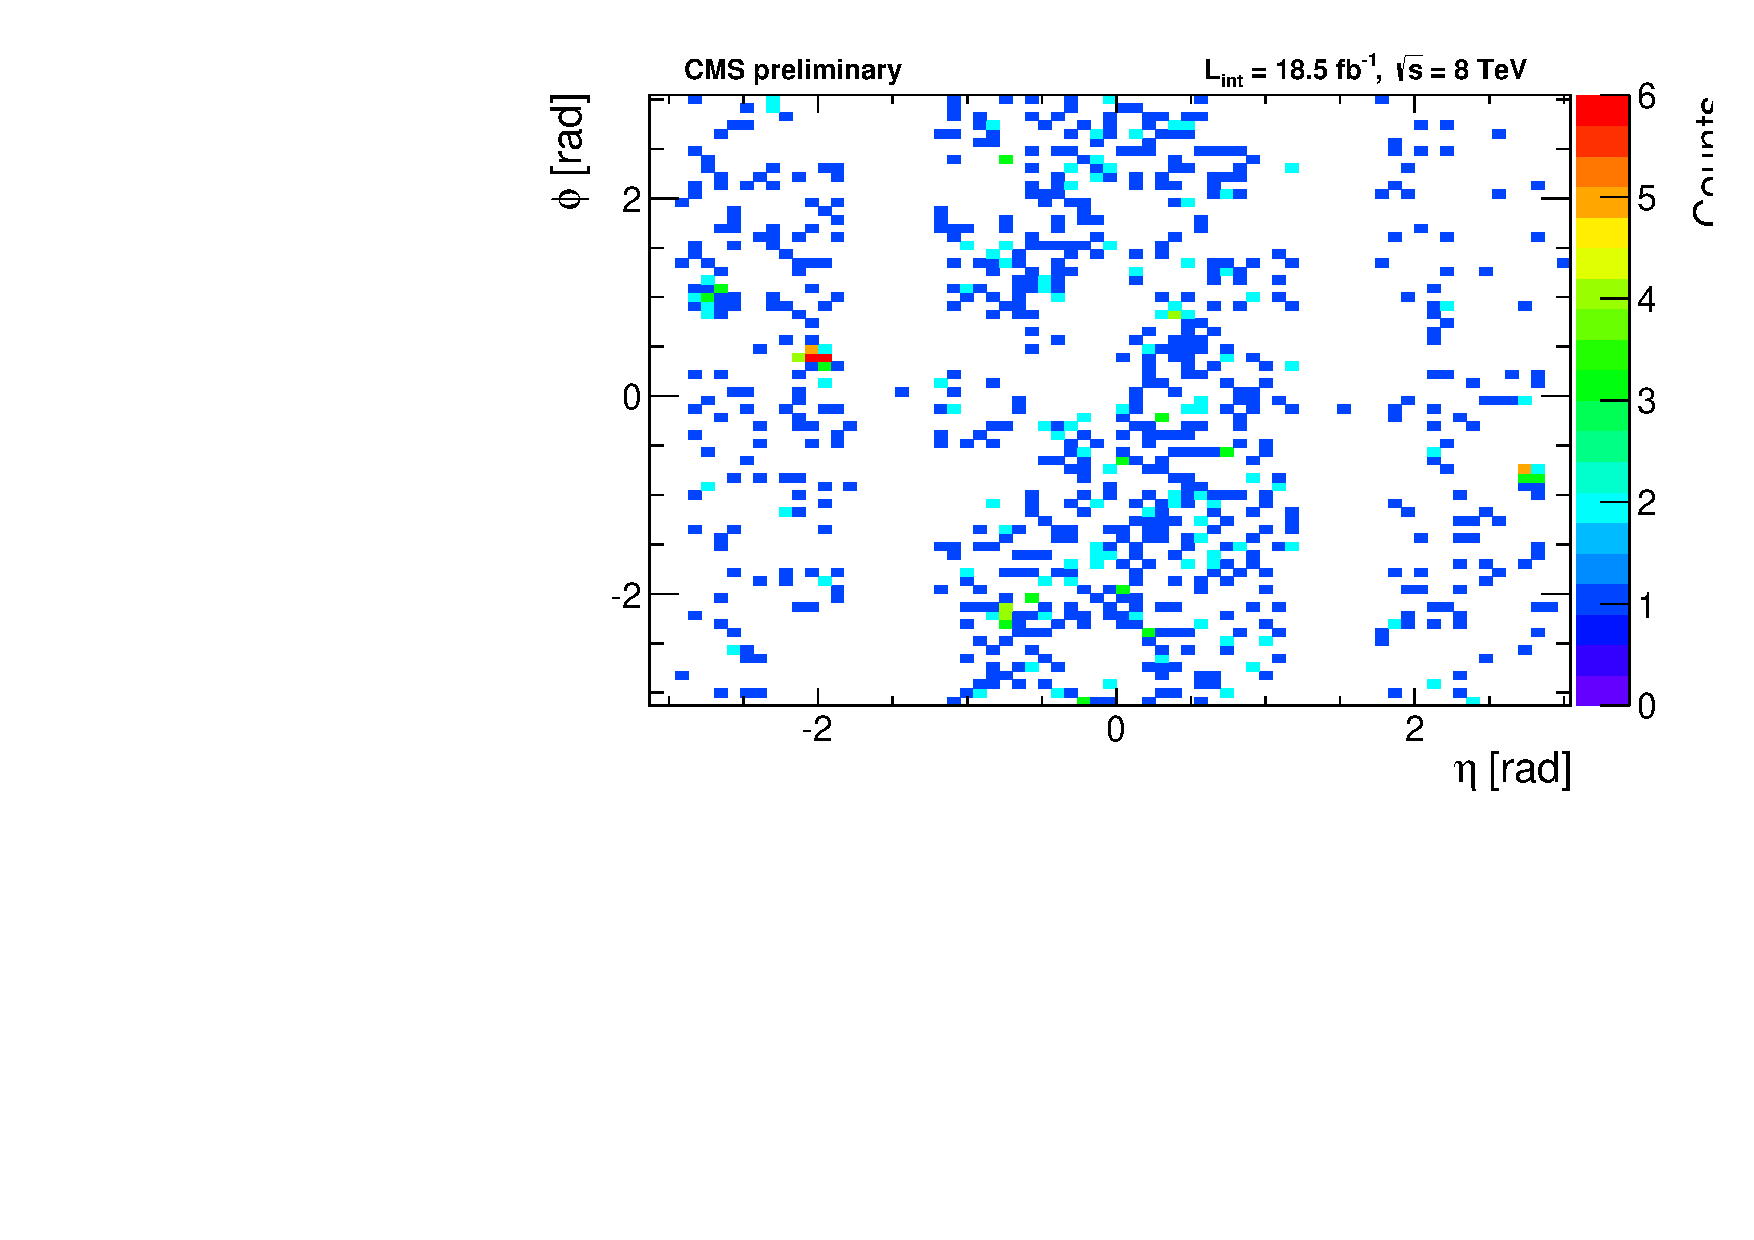
\includegraphics[width=\textwidth]{Figs/dphi/Nominal_AlphaT_thresholds/th2d_numer_summed_ge2j_ge0b_200.pdf}
      \caption{With ``dead ECAL filter''.}
      \label{fig:hotspots_2d_withdeadECAL}
    \end{subfigure}
    \begin{subfigure}[b]{0.46\textwidth}
      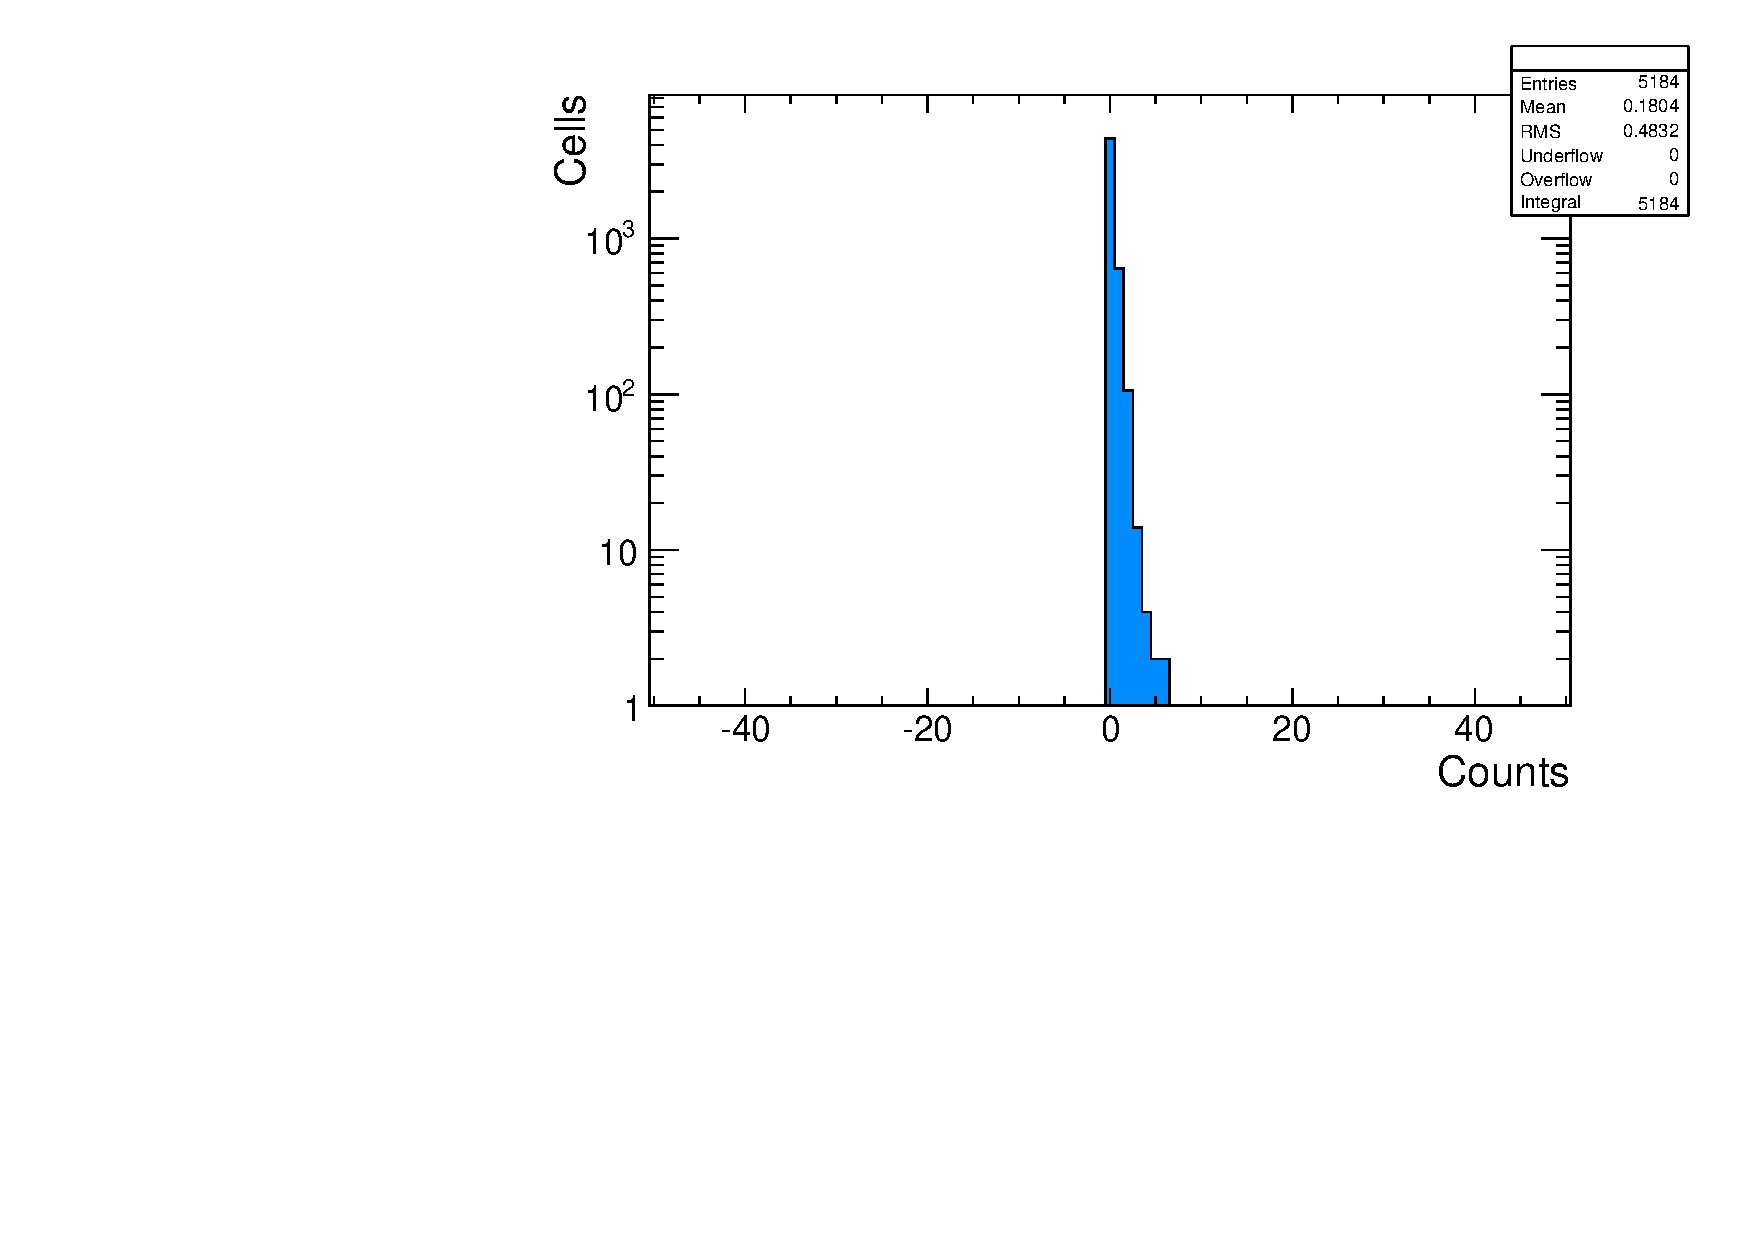
\includegraphics[width=\textwidth]{Figs/dphi/Nominal_AlphaT_thresholds/th1d_numer_summed_ge2j_ge0b_200.pdf}
      \caption{With ``dead ECAL filter''.}
      \label{fig:hotspots_1d_withdeadECAL}
    \end{subfigure} \\ 
    \caption{Distribution of jets in ($\eta$,$\phi$)-space that are
      responsible for an event satisfying the requirement $\dphistar <
      0.3$, with (a,b) and without (c,d) the ``dead ECAL filter''
      requirement applied as part of the signal region selection.}
    \label{fig:hotspots}
  \end{center}
\end{figure}

\subsection{Heavy-flavour jet decays}
\emph{This section is still a work in progress and will be updated inline with
our analysis note.}

Jets can also appear to be mis-measured if they contain the parton
shower contains heavy flavour mesons which decay leptonically. In rare
circumstances, these decays can give the largest fraction of the available
momenta to the neutrino, leading to significant amounts of real \met and
soft-leptons which evade the lepton vetoes (see appendix~\ref{ch:app_dphistar}).
This effect is compounded when multiple neutrinos are produced in the shower,
with a significant fraction of the jet's energy is invisible.

To better study events of this type a control sample is defined, based on using
the single-object \HT trigger, \verb!HLT_HT750!, which remained un-prescaled
throughout \runone. As opposed to the typical signal trigger, the lack of an
\alphat requirement allows lower regions of \alphat to be studied. The region is
therefore defined by \HT > 775 \gev and \alphat > 0.507, where this trigger is
full efficient. Due to the intrinsic correlation of \HT and \mht in the \alphat
variable (figure~\ref{fig:alphat_mht_corr}), this selection leads to an
effective \mht requirement similar to that of the low \HT categories of the
nominal analysis.

Events containing jets containing real \met sources are likely to have
$\mht \approx \met$, and would therefore not be protected against by the \mhtmet
described in section~\ref{sec:qcd_cleaning_below_thresh}. Consider the ratio
of events passing and failing the \mhtmet requirement:
% 
\begin{equation}
\label{eq:rmhtmet}
\rmhtmet = \frac{N(\mhtmet<1.25)}{N(\mhtmet>1.25)}.
\end{equation}
% 
This variable is plotted as a function of \alphat with the predicted EWK
background (as determined using the method outlined in
chapter~\ref{ch:background})
subtracted, leaving only QCD multijet events.
In the absence of events with jets containing real \met a strong
exponential decrease would be expected. However, given these events populate the
\mhtmet < 1.25 region, a constant pedestal is observed REF REF, leading to the
conclusion of residual QCD contamination in the signal region.

\emph{rmhtmet plots!}

Jets containing a \met source appear to be mismeasured and will therefore
populate a region of low \dphistar.
Figure~\ref{fig:qcd_region_pred_dphistar_incl} shows the data compared to the
EWK background prediction (this method is discussed later in
chapter~\ref{ch:background})
as a function of the \mindphistar value of each event. The disagreement observed
at low \mindphistar is well accounted for by the yield from QCD MC. It should be
noted that while MC can be relied on for a qualitative understanding of the QCD
contamination, it should not be used to determine a quantitative understanding
of the phenomenon.

\begin{figure}
  \centering
  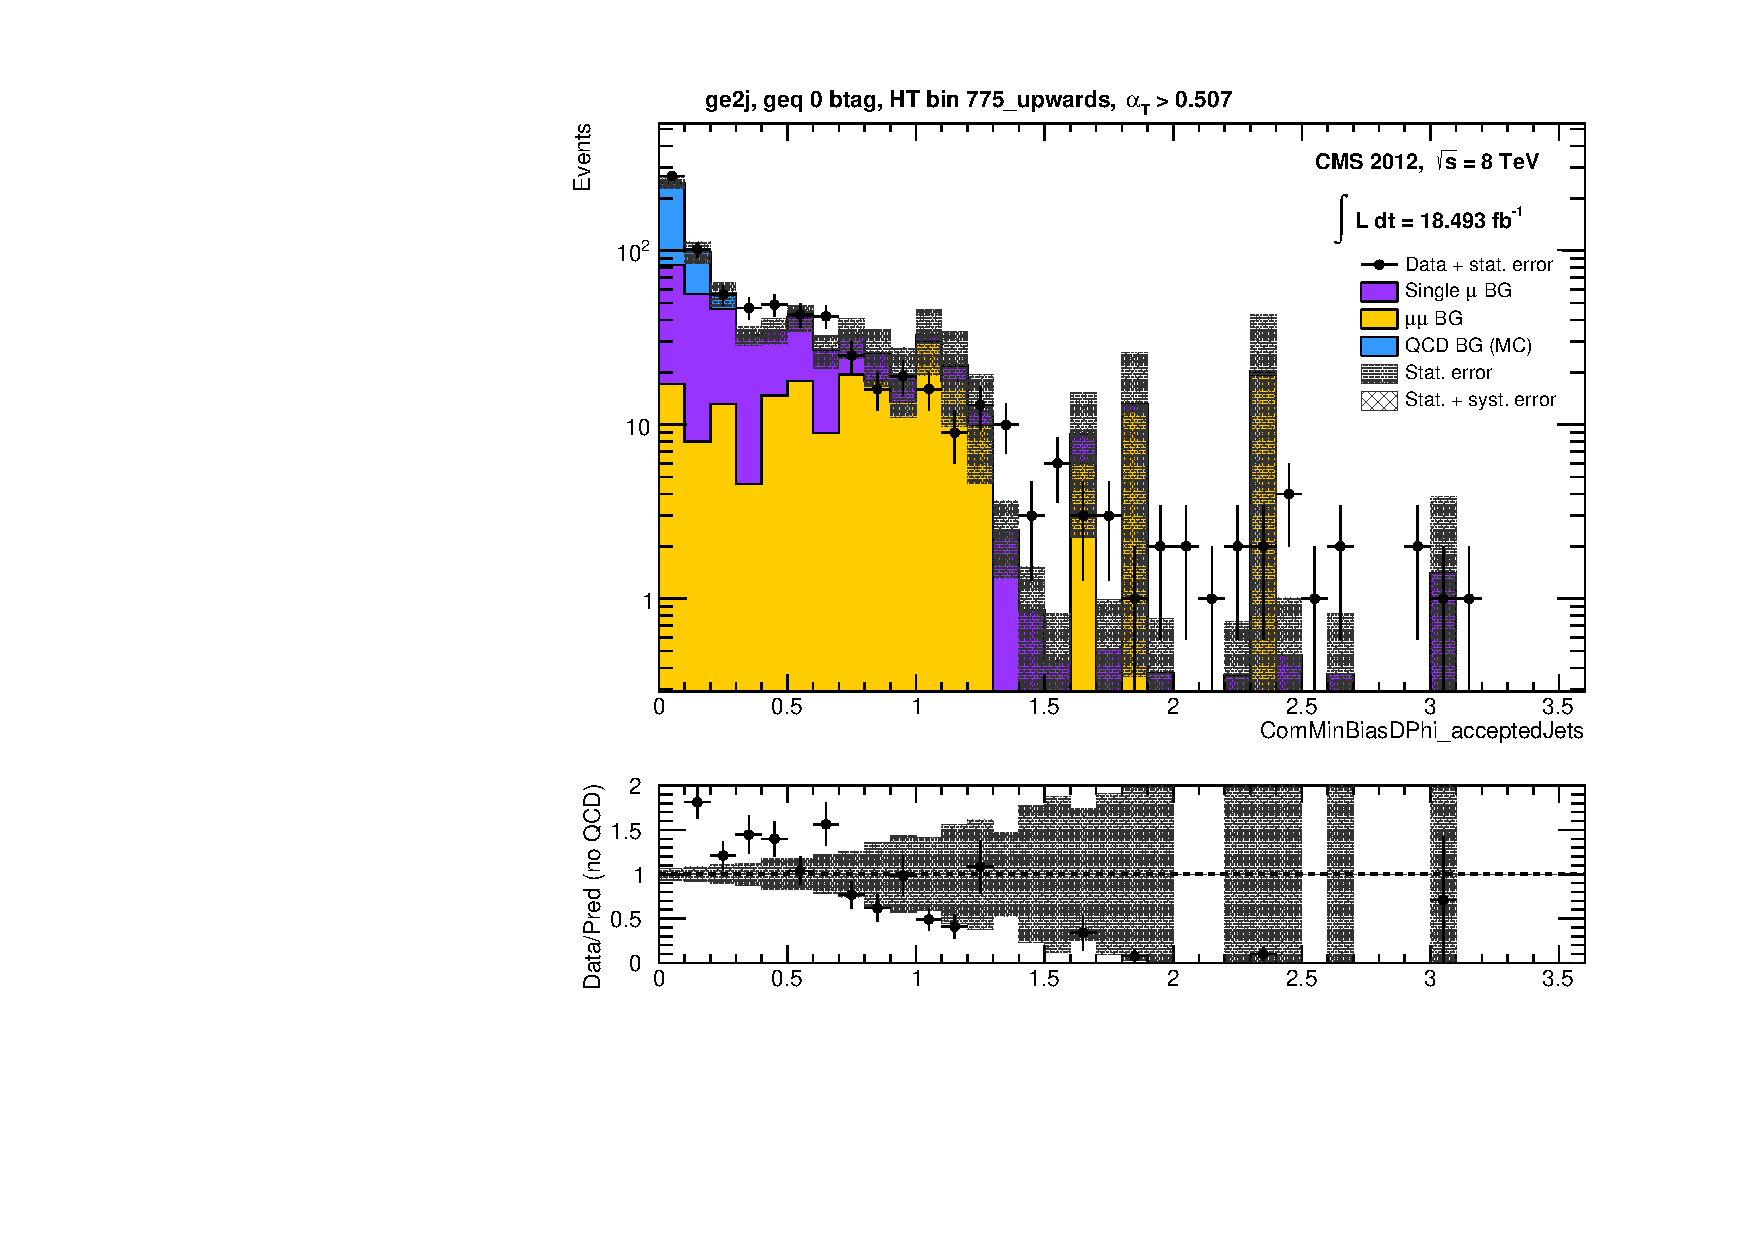
\includegraphics[width=0.6\textwidth]
  {Figs/datapred/qcd_study_region/ge2j_ge0b_775_upwards/Prediction_ComMinBiasDPhi_acceptedJets_all_775_upwards_QCD}
  \caption{Data (black points) against the EWK background prediction 
  (stacked, yellow and purple) as a function of \mindphistar. The expected yield
  from QCD MC (cyan) is stacked on top of the EWK prediction. The plot represents
  the QCD control study region, with $\nb \geq 0$, $\nj \geq 2$, $\HT > 775
  \gev$ and $\alphat > 0.507$.}
  \label{fig:qcd_region_pred_dphistar_incl}
\end{figure}

As motivated by figure~\ref{fig:qcd_region_pred_dphistar_incl}, the residual QCD
events appear to be well isolated in the region $\mindphistar < 0.3$. The effect
of applying this threshold in the QCD control study region is shown in
figure~\ref{fig:data_pred_dphistar_eff}. The $\dphistar > 0.3$ requirement
removes these events entirely (CHECK!).

\begin{figure}[h!]
  \centering
  \begin{subfigure}[b]{0.46\textwidth}
    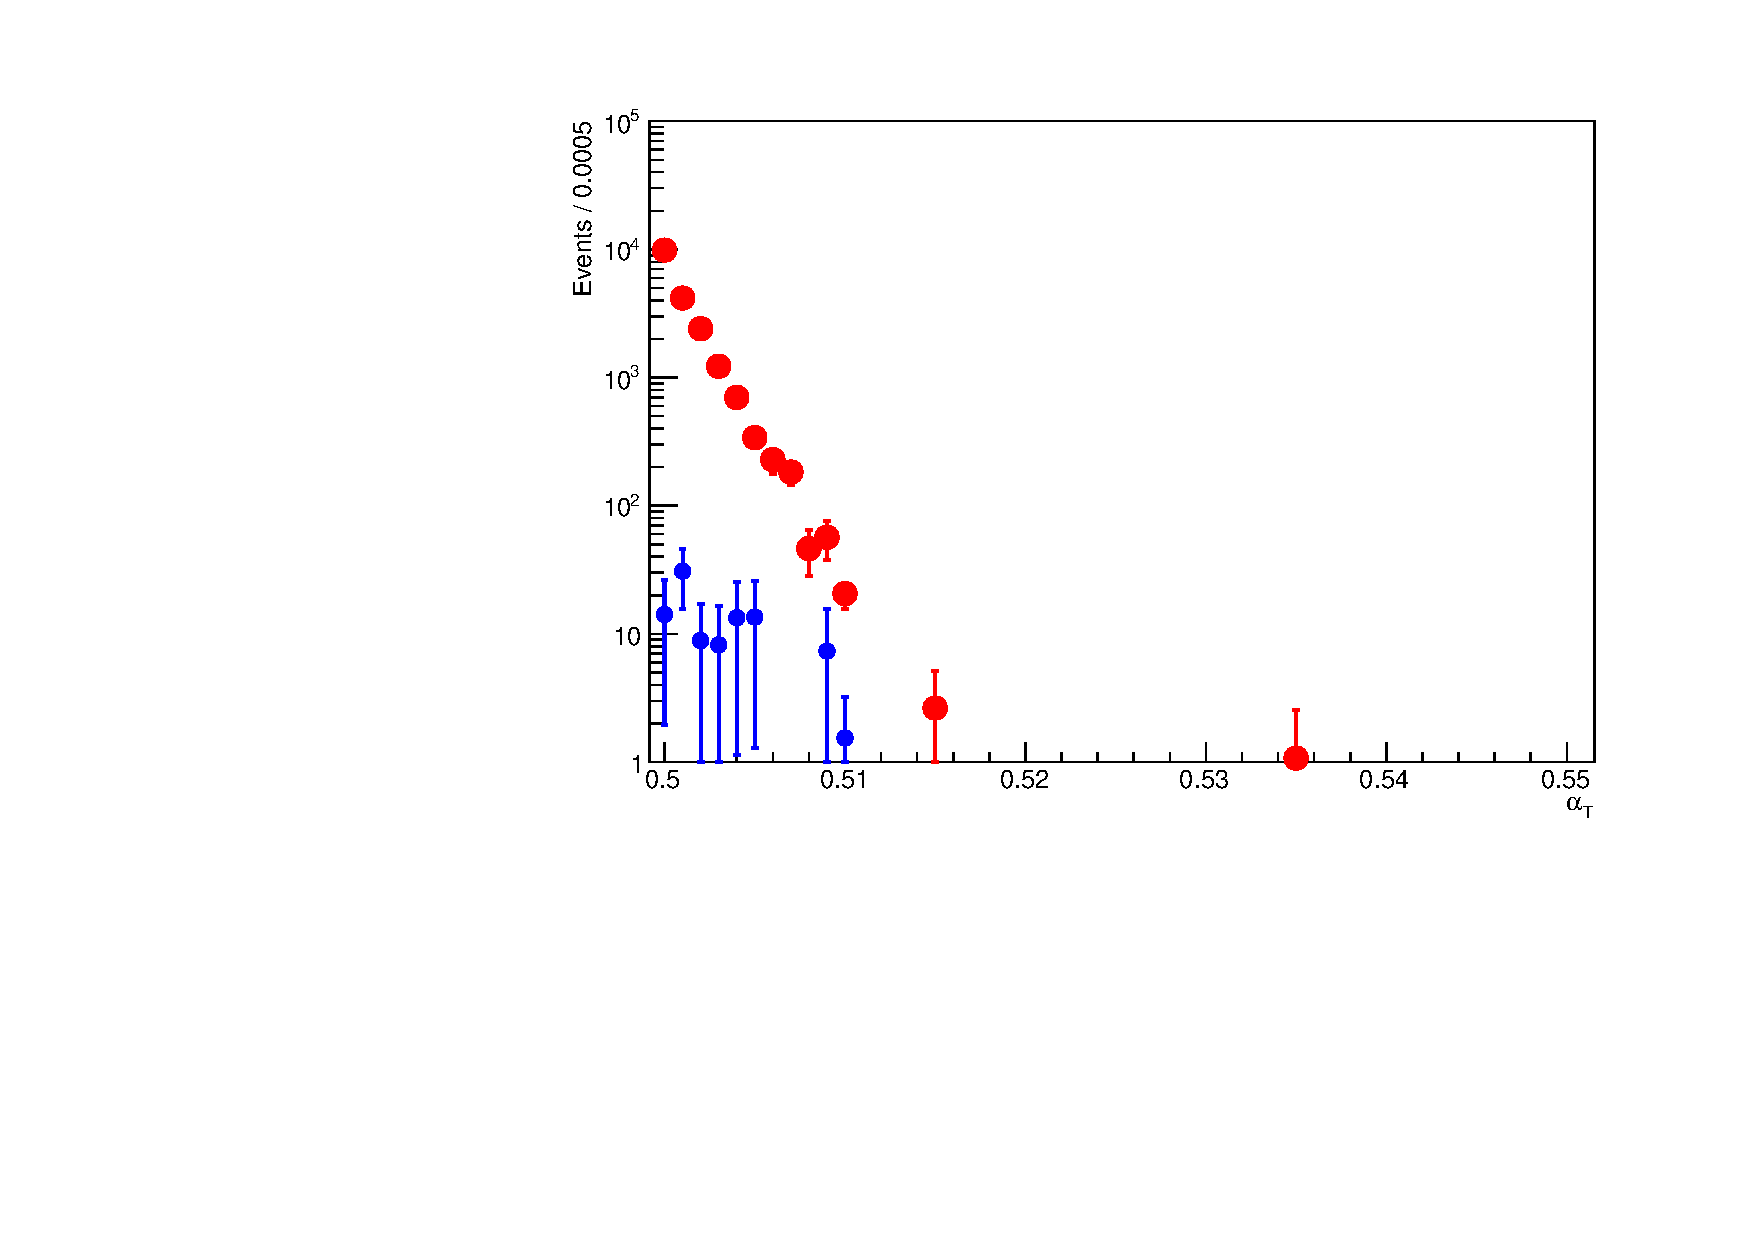
\includegraphics[width=\textwidth]{Figs/dphi/chris2/qcd_mc/dphi_incl/dphi_eq3j_ge0b_775}
    \caption{$\nj = 3$, simulation}
    \label{fig:dphi_acceptance_sim_3j}
  \end{subfigure}
  \begin{subfigure}[b]{0.46\textwidth}
    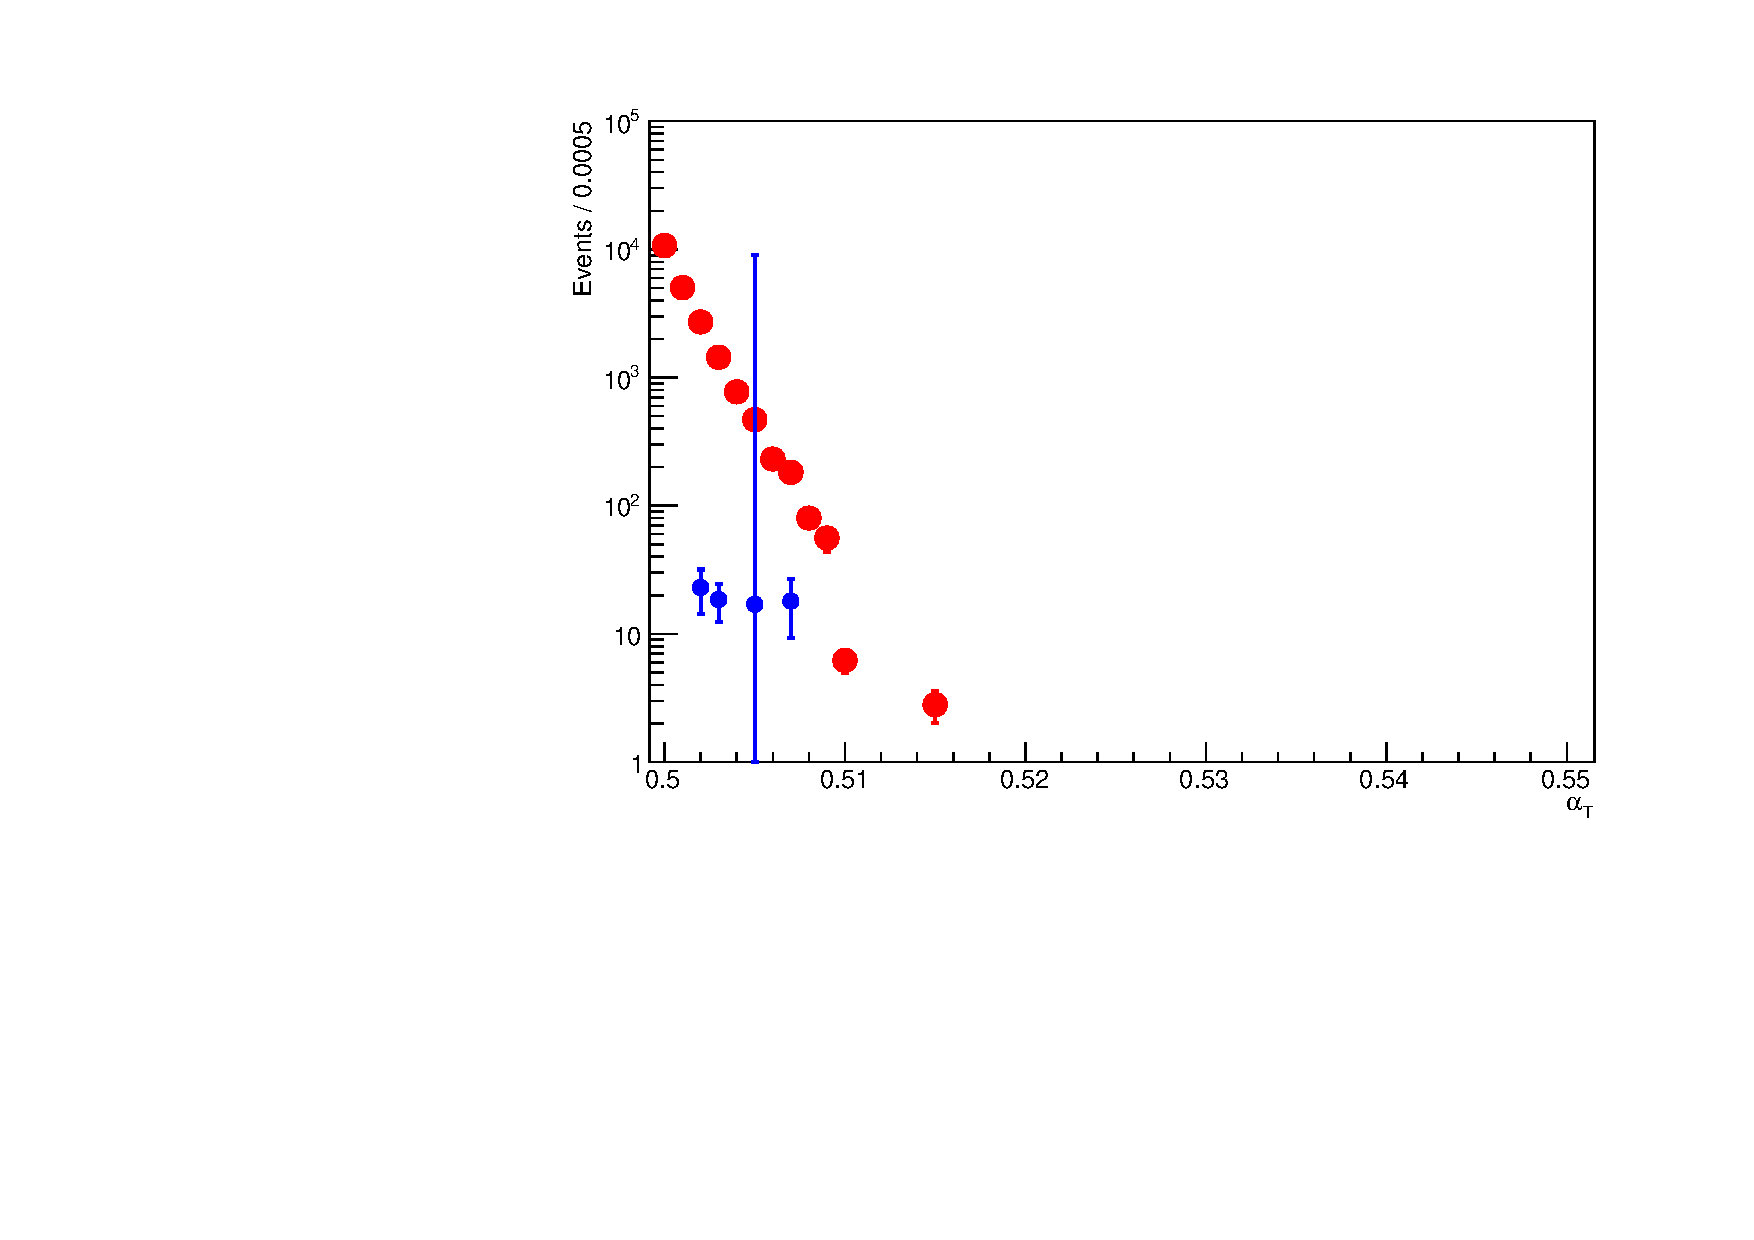
\includegraphics[width=\textwidth]{Figs/dphi/chris2/data/dphi_incl/dphi_eq3j_ge0b_775}
    \caption{$\nj = 3$, data}
    \label{fig:dphi_acceptance_data_3j}
  \end{subfigure}\\
  \begin{subfigure}[b]{0.46\textwidth}
    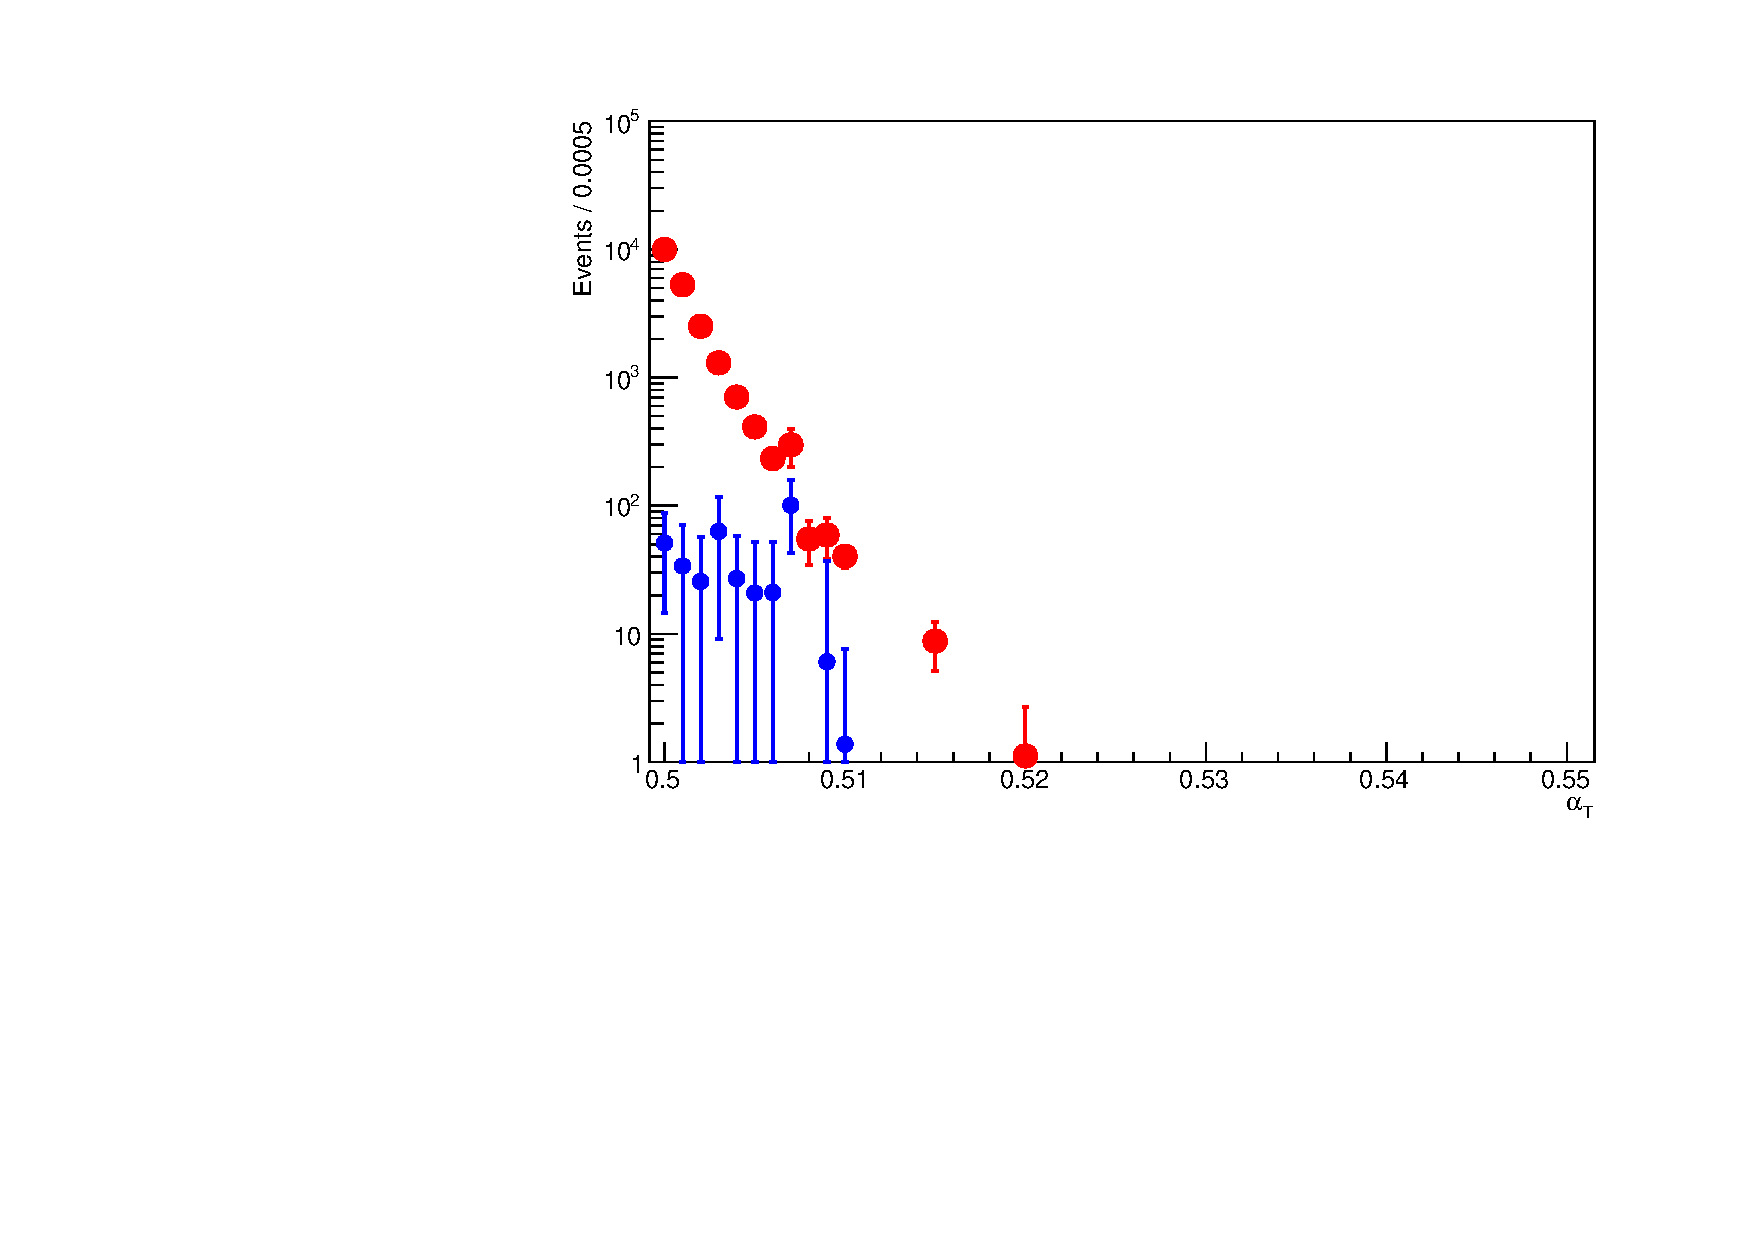
\includegraphics[width=\textwidth]{Figs/dphi/chris2/qcd_mc/dphi_incl/dphi_eq4j_ge0b_775}
    \caption{$\nj = 4$, simulation}
    \label{fig:dphi_acceptance_sim_4j}
  \end{subfigure}
  \begin{subfigure}[b]{0.46\textwidth}
    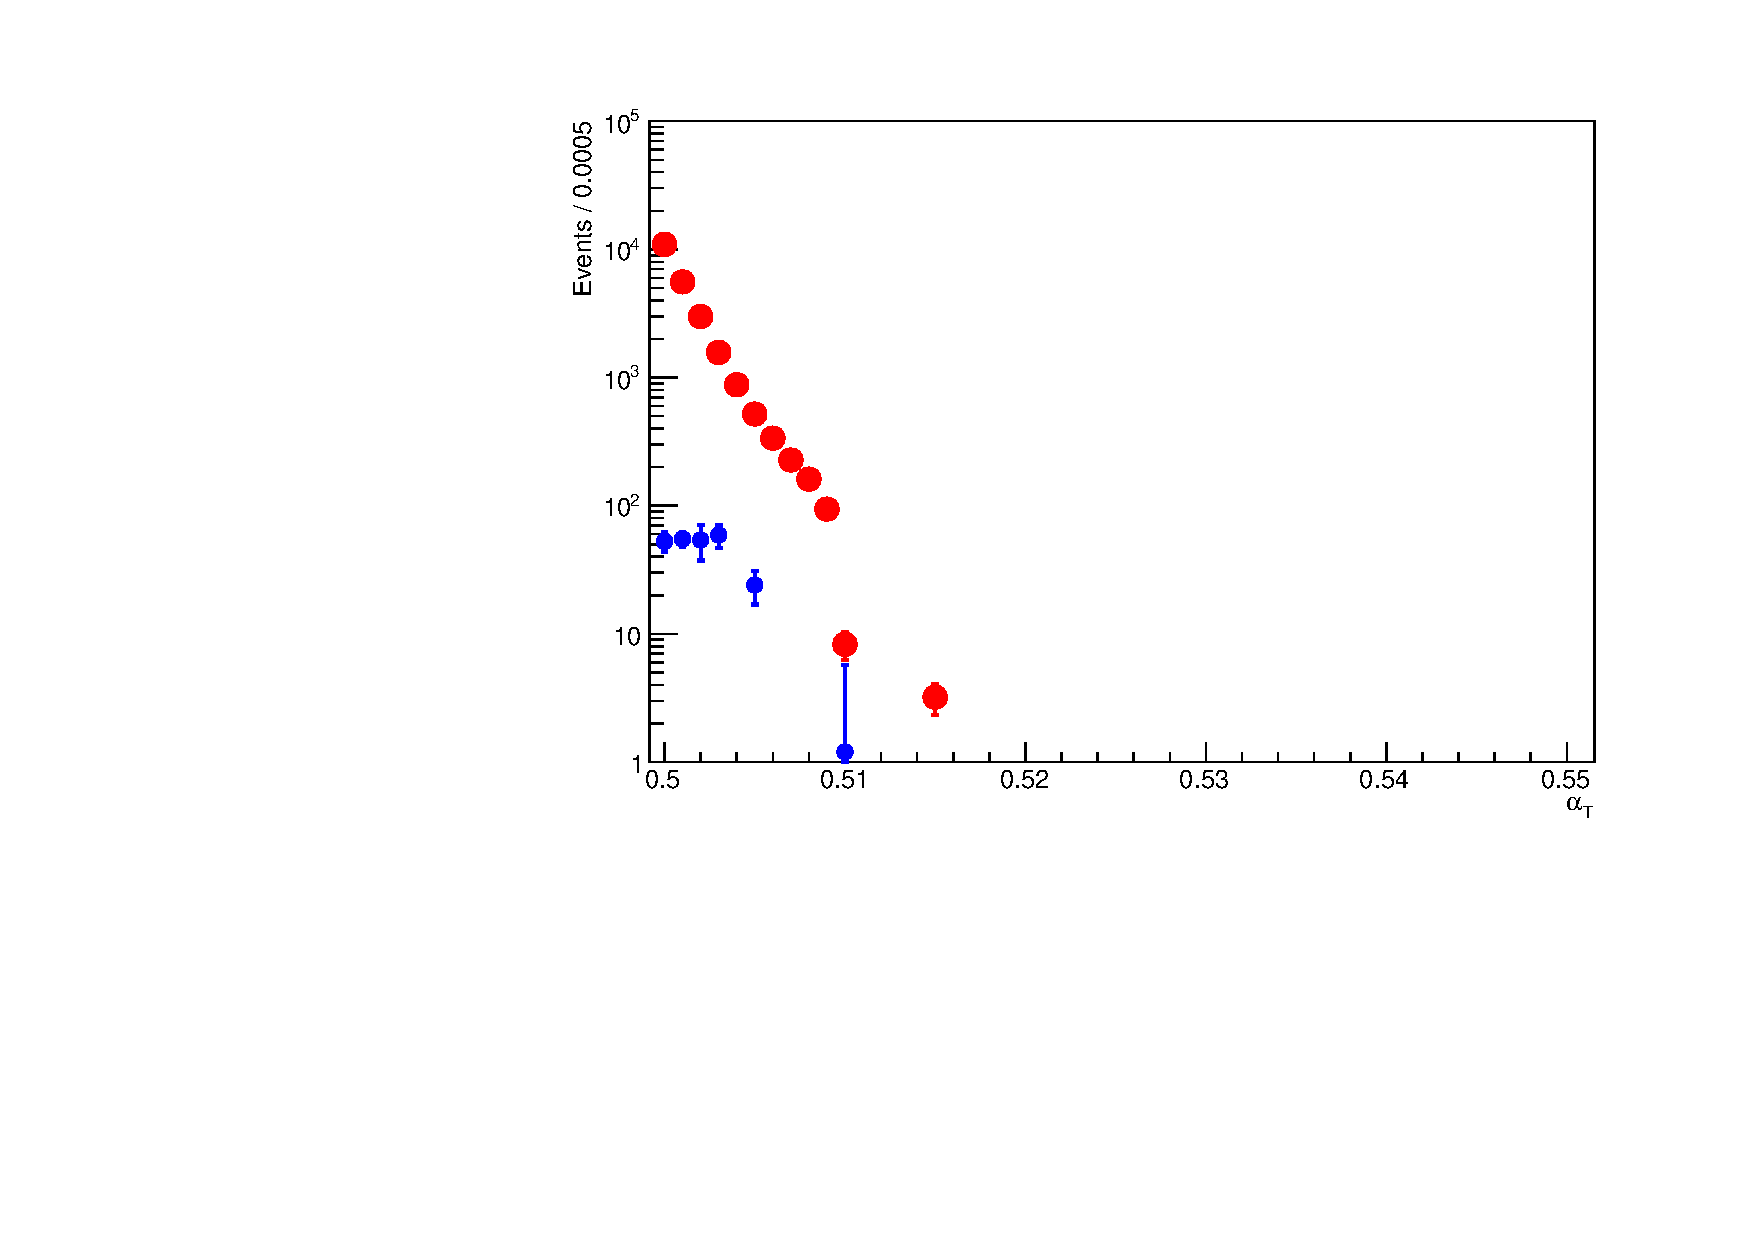
\includegraphics[width=\textwidth]{Figs/dphi/chris2/data/dphi_incl/dphi_eq4j_ge0b_775}
    \caption{$\nj = 4$, data}
    \label{fig:dphi_acceptance_data_4j}
  \end{subfigure}\\
  \caption{The \alphat distribution for events with no \dphistar
    requirement (red circles) and with the $\dphistar > 0.3$
    requirement (blue circles) as determined from QCD multijet
    simulation (left column) or data (right column) and the exclusive
    $\nj =3$
    (top row) or $\nj = 4$ (bottom row). The QCD control study region
    requirements have been applied, $\HT > 775$ \gev and $\alphat > 0.507$, with
    $\nb \geq 0$.}
    \label{fig:data_pred_dphistar_eff}
\end{figure}

\emph{R(MHTMET) plots}

\emph{dphistar pass/fail plots}

Events are required to have \dphistar > 0.3, in
order to clean any remaining events with jets containing sources of genuine \met jet (see
appendix~\ref{ch:app_dphistar}).

% For bins of $\HT>375$ \gev the leading two jets in the event are required to 
% have $\Pt>100$ \gev, with all additional jets having half the requirement of
% $\Pt>50$ \gev. In order to maintain a similar kinematic phase space throughout
% the many \HT bins, these jet \Pt requirements are scaled for the lower \HT bins 
% as shown in Table~\ref{tab:jet_pt_thresholds}.

\section{Predicting high-\nb event yields}
\label{sec:formula_method}

Determining yields for high-\nb analysis categries directly from simulation
becomes
inherently reliant on not only MC modelling, but also on the physics
distribution of jet-flavours. For EWK samples, given the underlying abundance of
low b-jet multiplicity events, high-\nb categories become dominated by
mis-tagging of light-flavour jets, leading to large statistical uncertainties.
In order to reduce this reliance on direct MC yields, a method has been
developed REF using flavour tagging efficiencies and the underlying quark
flavour distribution, both measured directly from simulation in order to
statistically determine more precise yields, particularly for the high-\nb
categories.

This method and it's validation are described in detail in REF. The approach can
be summarised by:
% 
\begin{equation}
\begin{split}
N(n) = \sum_{n_b^{gen} + n_c^{gen} + n_{\text{light}}^{gen} = n_{jet}^{cat}}\:
\sum_{n_b^{tag} + n_c^{tag} + n_{\text{light}}^{tag} = n}
N(n_b^{gen}, n_c^{gen}, n_q^{gen}) \times \\
P(n_b^{tag}, n_b^{gen}, \epsilon_{b}) \times
P(n_c^{tag}, n_c^{gen}, \epsilon_{c}) \times
P(n_{\text{light}}^{tag}, n_{\text{light}}^{gen}, \epsilon_{\text{light}}) ,
\end{split}
\end{equation}
% 
where $N(n)$ is represents the predicted yield of $n$ b-tagged events for a
given
analysis category and \HT bin. The jet-flavour tagging probability
terms $P(n_b^{tag}, n_b^{gen}, \epsilon_{b})$,
$P(n_c^{tag}, n_c^{gen}, \epsilon_{c})$ and 
$P(n_{\text{light}}^{tag}, n_{\text{light}}^{gen}, \epsilon_{\text{light}})$ are measured for each \HT bin and
analysis category for each simulated sample, including the flavour tagging
effiencies $\epsilon_b$, $\epsilon_c$ and $\epsilon_{\text{light}}$ as also measured from
each sample. Finally, $N(n_b^{gen}, n_c^{gen}, n_q^{gen})$ represents the
distribution of actual generator-level jet flavours in the events.

In the large-statistic sample limit this technique would not be necessary,
as enough high-\nb events would be present to sufficiently reduce statistical
uncertainties. However, in the absence of this un-feasible scenario,
this technique
makes uses of all events in a sample, thereby reducing the uncertainties
and ultimately delivering more precise yields from simulation.


\section{Example distributions and cutflow}

Example distributions from MC simulations of \alphat, \HT, \mht and jet \Pt  are
shown in figure~\ref{fig:datamc_had_inc}.

\begin{figure}[!ht]
  \centering
    \begin{subfigure}[b]{0.48\textwidth}
      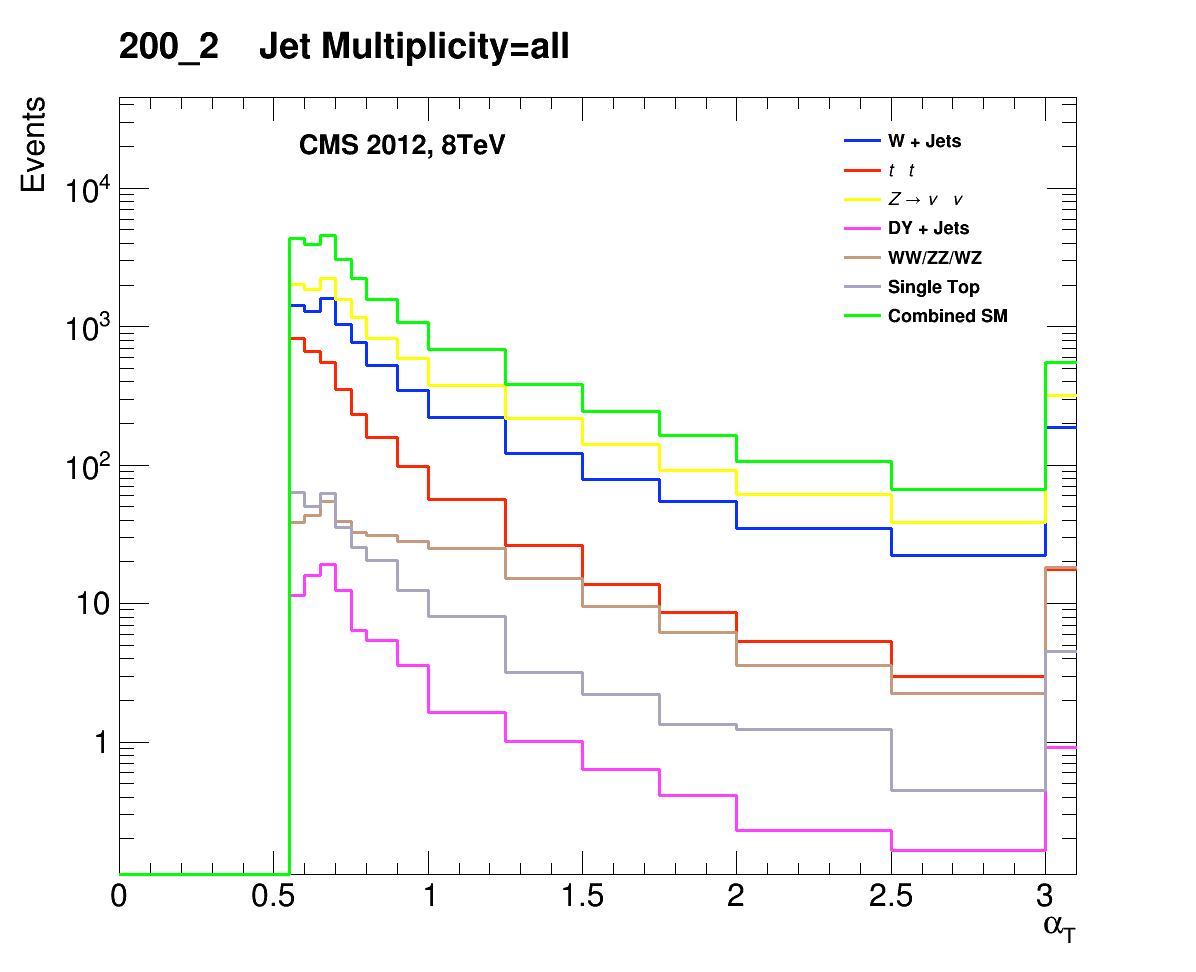
\includegraphics[width=\textwidth]{Figs/datamc/had/v1/AlphaT_all_200_upwards}
      \caption{\alphat}
    \end{subfigure}
    \begin{subfigure}[b]{0.48\textwidth}
      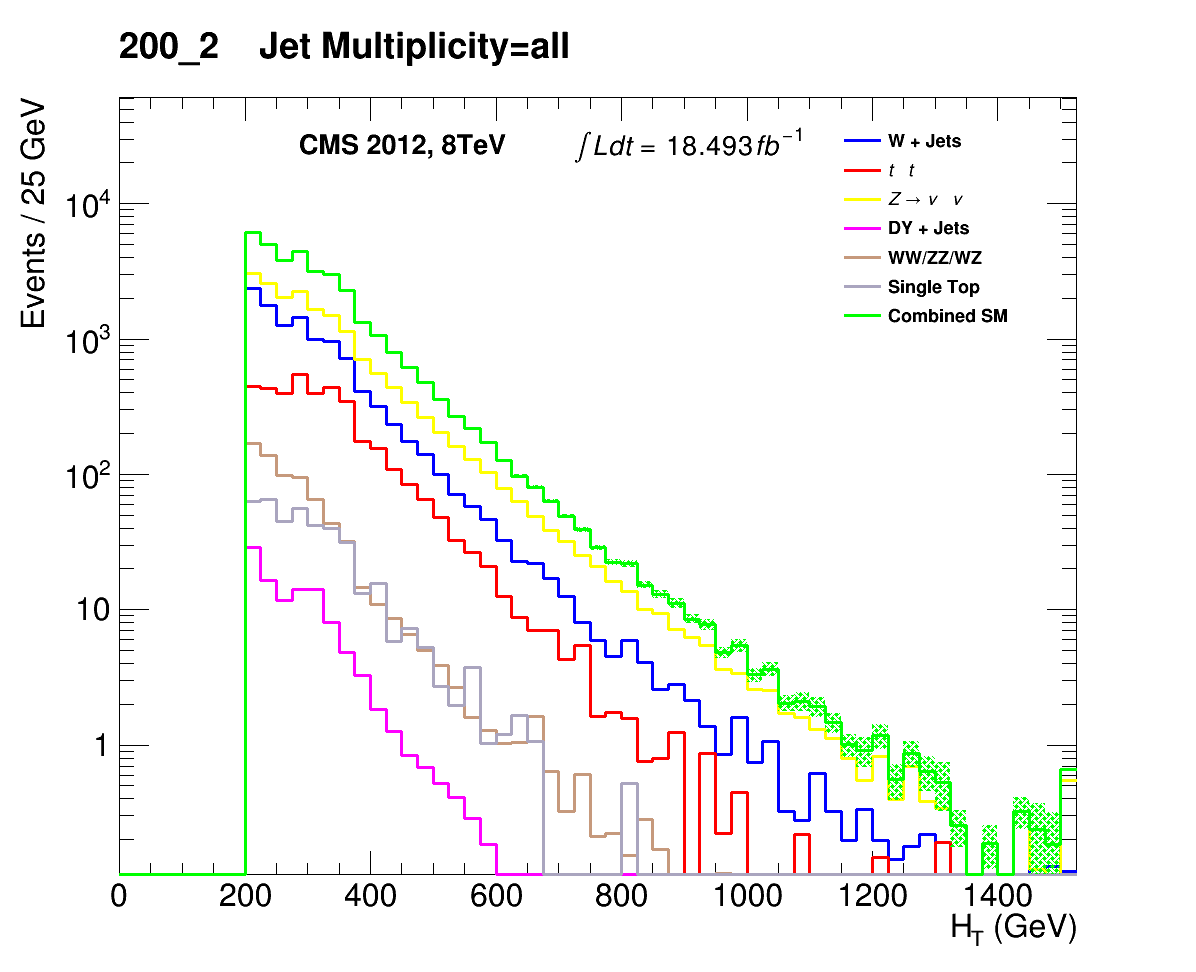
\includegraphics[width=\textwidth]{Figs/datamc/had/v1/HT_all_200_upwards}
      \caption{\HT}
    \end{subfigure} \\
    \begin{subfigure}[b]{0.48\textwidth}
      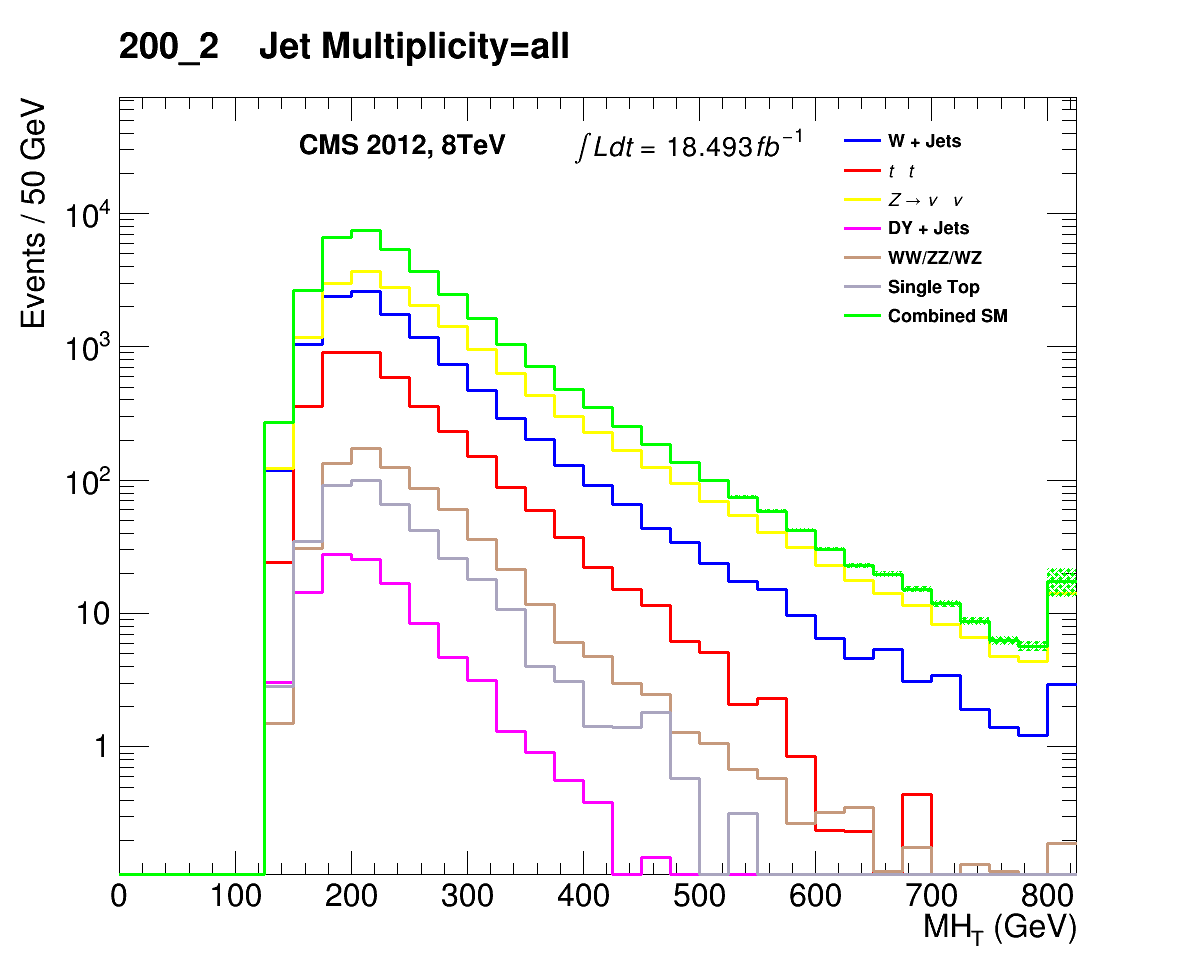
\includegraphics[width=\textwidth]{Figs/datamc/had/v1/MHT_all_200_upwards}
      \caption{\mht}
    \end{subfigure}
    \begin{subfigure}[b]{0.48\textwidth}
      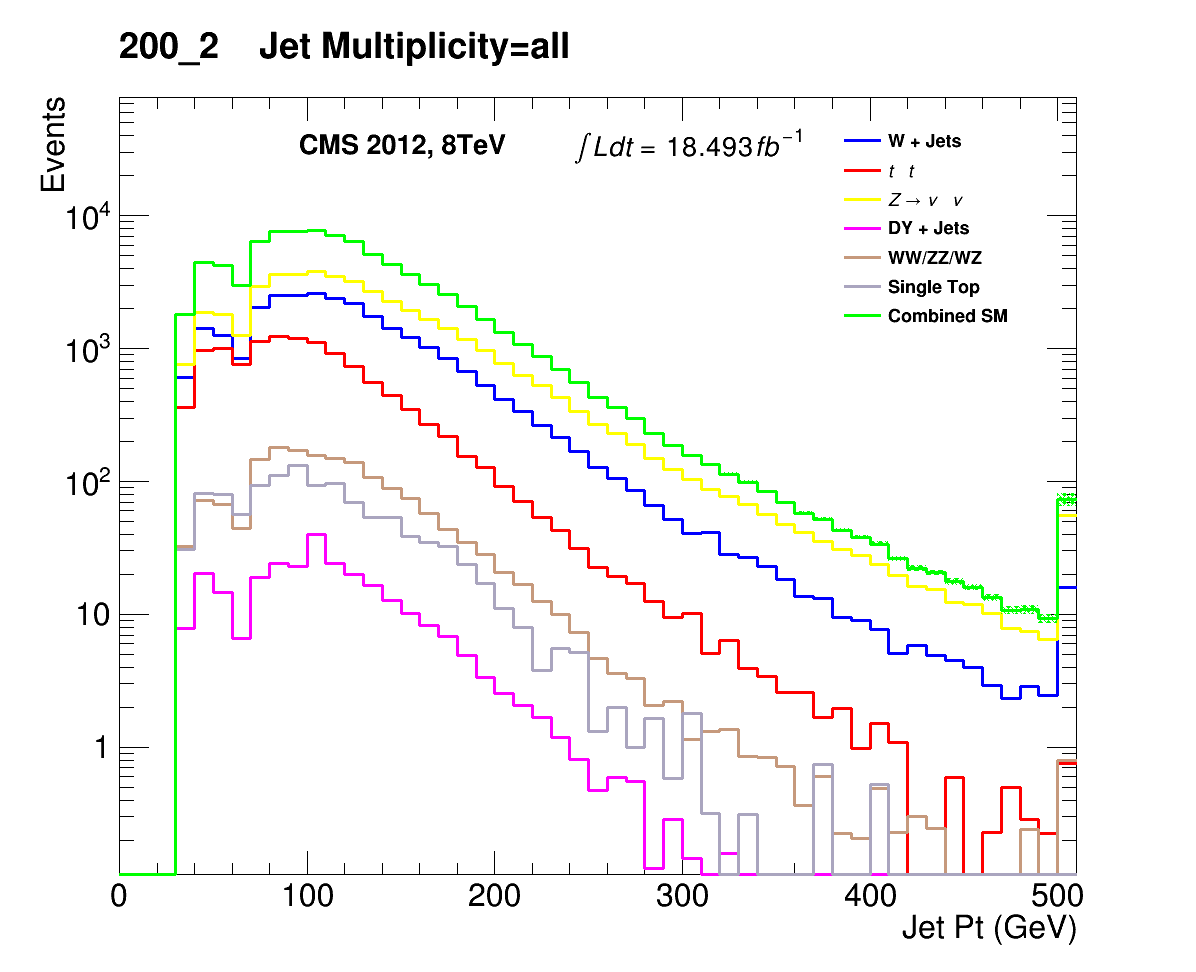
\includegraphics[width=\textwidth]{Figs/datamc/had/v1/CommonJetPt_all_200_upwards}
      \caption{Jet \Pt}
    \end{subfigure} \\
    \caption{\label{fig:datamc_had_inc}
    MC distributions for the full hadronic signal selection. The 
    sum of the individual sample contributions is shown in green. Plots
    are for $\HT>200$ \gev, $\nj\geq2, \nb\geq0$.
    }
\end{figure}
  
The cutflow yields are shown in table~\ref{tab:had_data_cutflow} for data in the
\HT > 375 \gev region, with an inclusive selection on \nj and \nb.

\begin{table}[ht!]
  \caption{The cutflow of the hadronic selection in data. The subscript `fail'
  indicates an object which did not meet all ID requirements, and so is not
  considered as a `common object'. The event selection follows an inclusive
  selection in data of $\HT > 375$ \gev, $\nj \geq 2$ and $\nb \geq 0$. }
  \label{tab:had_data_cutflow}
  \centering
  \footnotesize
  \begin{tabular}{ lcc }
    \hline
    \hline
    Cut Name    & Eff (\%) & N \\
    \hline
  Event Count  & 100.00  & 161866108.00 \\
  Good Event JSON Filter  & 94.97  & 153716716.00 \\
  $\nj \geq 2$  & 98.68  & 151689664.00 \\
  MET Filters & 98.81  & 149885013.00 \\
  Vertex Noise Filter & 99.91  & 149746017.00 \\
  DeadECAL Filter & 35.44  & 53066597.00 \\
  Select seed Trigger & 3.76  & 1995549.00 \\
  $n_{e} = 0$ & 98.48  & 1965269.00 \\
  $n_{\gamma} = 0$  & 97.70  & 1920124.00 \\
  $n_{\mu} = 0$ & 98.36  & 1888711.00 \\
  $\text{EMF}_{max}$ for all jets > 0.1 & 99.99  & 1888576.00 \\
  Leading jet \Pt > 100 \gev  & 97.83  & 1847501.00 \\
  Leading jet $\eta$ < 2.5  & 97.31  & 1797777.00 \\
  Sub-Leading jet \Pt > 100 \gev  & 81.75  & 1469654.00 \\
  $n_{jet, fail} = 0$ & 81.73  & 1201096.00 \\
  $\Delta R(\mu^i_{fail}, jet^j) < 0.5$ & 98.77  & 1186370.00 \\
  $(\sum_{}^{n_{vertices}}{\Pt}$) / \HT & 100.00  & 1186368.00 \\
  recHitCut & 98.44  & 1167861.00 \\
  $n_{SIT} = 0$ & 85.77  & 1001646.00 \\
  \mindphistar > 0.3  & 19.50  & 195361.00 \\
  \HT > 375 \gev  & 73.33  & 143255.00 \\
  \mhtmet < 1.25  & 9.26  & 13263.00 \\
  \alphat > 0.55  & 38.25  & 5073.00 \\
    \hline
    \hline
  \end{tabular}
\end{table}







\chapter{Background Estimation}
\label{ch:background}

% **************************** Define Graphics Path **************************
\ifpdf
    \graphicspath{{Chapter6/Figs/Raster/}{Chapter6/Figs/PDF/}{Chapter6/Figs/}}
\else
    \graphicspath{{Chapter6/Figs/Vector/}{Chapter6/Figs/}}
\fi

Predictions of EWK SM backgrounds are made using independent control regions
designed to mimic a specific background process observed in the signal region.
These regions are orthogonal to the signal region due to the
selection of leptons or photons - particles which are subsequently ignored such 
that the selection kinematics of each event is kept similar to the corresponding
process. For each sample, Transfer Factors (TF) are 
constructed from yields in MC, to extract a prediction in the signal 
region for a given process. This process is described at length in
section~\ref{sec:background_overview}. The validity of this procedure is
extensively tested using a suite of Closure Tests, probing multiple
characteristics of the prediction technique while allowing for \HT-dependent
systematic errors to be derived on the prediction.

Predictions made using this technique alone are considered as ``primitive'' 
predictions and are used only in analysis development and the derivation of 
background systematics. In order to determine final background counts for
interpretation and
limit-setting, a fit is made across all signal and control regions, using the 
likelihood model as described later in chapter~\ref{ch:results}. The derived 
transfer factors and individual yields enter as terms in the likelihood, where 
all related systematics, potential correlations and signal contamination are
accounted for.

Residual contamination from QCD processes are removed through additional
cleaning cuts. Studies performed in a QCD enriched sideband region in \alphat
lead to the definition of these cuts, as described in
section~\ref{sec:qcd_cleaning}, ensuring no significant QCD remains.

% Thresholds of the \alphat variable are determined such that the QCD MJ 
% contribution to the SM background is negligible. These are found using a
% data-driven method, employing sidebands in both the \mhtmet and \alphat variables, 
% described in section~\ref{sec:background_qcd}. Following the 
% application of these thresholds, any QCD contributions are considered negligible
% and are therfore not considered in the likelihood model.

%********************************** % First Section  *************************************
\section{Overview of Electroweak background prediction method}  %Section - 1.1 
\label{sec:background_overview}

% Contributions from Standard Model background processes are estimated using a data-driven 
% prediction technique, employing dedicated control samples.
A transfer factor is constructed from MC samples as the ratio 
of the yield in the signal region, \\$N_{MC}^{signal}\big(\HT, \nj, \nb\big)$,
and the yield of a given control region, \\$N_{MC}^{control}\big(\HT, \nj,
\nb\big)$, as a function of the analysis binning, \HT, \nj and \nb, defined as:
% 
\begin{equation}
TF = \frac{N_{MC}^{signal}\big(\HT, \nj, \nb\big)}{N_{MC}^{control}\big(\HT, \nj, \nb\big)} .
\label{eq:transfer_factor}
\end{equation}
% 
For a given \HT, \nj and \nb bin, the TF is used to extrapolate a yield in data from
the control region, $N_{data}^{control}\big(\HT, \nj, \nb\big)$,
to give a prediction in the signal region $N_{pred}^{signal}\big(\HT, \nj,
\nb\big)$, using:
%
\begin{equation}
N_{pred}^{signal}\big(\HT, \nj, \nb\big) = N_{data}^{control}\big(\HT, \nj, \nb\big)
\times TF .
\label{eq:transfer_equation}
\end{equation}
% 
The control samples are statistically independent and each used for predicting 
specific background processes.

MC yields are defined by process from the following samples:
W + jets (\numw),
\ttbar + jets (\numtt), DY + jets (\numdy), $\gamma$ + jets(\numgam),
single top + jets (\numtop), WW + jets, WZ + jets and ZZ + jets (\numdibo), and
\zinv + jets (\numzinv).

% Predictions made using this technique alone are considered as ``na\"{i}ve'' 
% predictions and are used only in analysis development and the derivation of 
% background systematics. In order to determine final yields for interpretation and 
% limit-setting, a fit is made across all signal and control regions, using the 
% full likelihood model, described later in chapter~\ref{ch:7}. The derived 
% transfer factors and individual yields enter as terms in the likelihood, where 
% all related systematics, potential correlations and signal contamination are
% accounted for in the fit. 

The denominator of each transfer factor is constructed using the sum of
\textit{all} MC sample yields, for a given control region and
analysis category:
% 
\begin{equation}
N_{MC}^{control}\big(\HT, \nj, \nb\big) = \numw + \numtt + \numdy + \numgam + 
\numtop + \numdibo + \numzinv .
\label{eq:trans_fact_denom}
\end{equation}
% 
The numerator is constructed according to the b tag multiplicity being 
considered. For $\nb \leq 1$, the \mj control region is used to predict 
lost-lepton background, e.g. \ttbar + jets and W + jets. All MC samples
are therefore used with the exception of \zinv + jets:
% 
\begin{equation}
N_{MC}^{signal}\big(\HT, \nj, \nb \leq 1\big) = \numw + \numtt + \numdy + \numgam + 
\numtop + \numdibo .
\label{eq:trans_fact_num_le1b_noz}
\end{equation}
% 
In this \nb region the \zinv + jets component of the background is predicted
with the \mmj and \gj control samples, using only the \zinv MC yields:
% 
\begin{equation}
N_{MC}^{signal}\big(\HT, \nj, \nb \leq 1 \big) = \numzinv .
\label{eq:trans_fact_num_le1b_z}
\end{equation}
%
For $\nb \geq 2$, the \mj sample is used to produce a prediction for all 
SM processes, including \zinv, and therefore the numerator of the TF is defined as:
% 
\begin{equation}
N_{MC}^{signal}\big(\HT, \nj, \nb \geq 2 \big) = \numw + \numtt + \numdy + \numgam + 
\numtop + \numdibo + \numzinv ,
\label{eq:trans_fact_num_geq2b}
\end{equation}
% 
or equivalently:
% 
\begin{equation}
N_{MC}^{signal}\big(\HT, \nj, \nb \geq 2 \big) = N_{MC}^{signal}\big(\HT, \nj, \nb \leq 1\big) + \numzinv .
\end{equation}

The \mmj and \gj control samples are not used beyond the $\nb \leq 1$ categories
due to the statistical limitations of such samples at high b tag multiplicities.
A full summary of the control regions used for predictions per analysis category
is shown in table~\ref{tab:control_prediction_summary}.

It should be noted that although two separate control samples are 
used to estimate the \zinv background contribution, the result of each is
considered by the global likelihood fit to produce the final background
prediction.

\begin{table}[ht!]
  \caption{The control samples used to produce SM background predictions for each 
  analysis category (\nb, \nj).}
  \label{tab:control_prediction_summary}
  \centering
  \small
  \begin{tabular}{ lll }
    \hline
    \hline
    \nj     & \nb     & Control samples \\ [1.0ex]
    \hline
    2--3    & 0       & \mj, \mmj, \gj  \\
    2--3    & 1       & \mj, \mmj, \gj  \\
    2--3    & 2       & \mj             \\
    $\geq$4 & 0       & \mj, \mmj, \gj  \\
    $\geq$4 & 1       & \mj, \mmj, \gj  \\
    $\geq$4 & 2       & \mj             \\
    $\geq$4 & 3       & \mj             \\
    $\geq$4 & $\geq4$ & \mj             \\
    \hline
    \hline
  \end{tabular}
\end{table}

By employing a technique that uses a ratio of MC yields, direct dependence on
MC modelling is 
greatly reduced. Sources of error inherent to MC samples, such as mismodelling effects, 
will cancel in the ratio. These errors can potentially include kinematic
mismodelling, which would affect analysis acceptance, and mismodelling of 
instrumental effects, which could affect object 
reconstruction efficiencies. However, any remaining systematics such as these
and others are probed using dedicated Closure Tests (CT), described in detail
in section~\ref{sec:closure_tests}.


%********************************** % Second Section  *************************************
\section{Control samples}  %Section - 1.2
\label{sec:background_control}

Control sample definitions are designed such that they are as kinematically
similar as possible
to the signal region, with the exception of a selected `tag' muon or 
photon. The `tagged' particle is then subsequently ignored for the calculation of all analysis 
variables, such as \HT, \met, \alphat etc.
Other differences include mass-window
and minor kinematic cuts, aimed at enriching the control samples in certain processes.
% The samples themselves are statistically independent, and orthogonal to the 
% signal region
Due to the selection of the tagged lepton or photon, the control samples are
orthogonal to the signal region and therefore minimise any
possible signal contamination. However, a full treatment of the
signal-contamination and sample cross-correlation is taken into account in the
background fit and final limit-setting. 

The following sections will describe the control regions in more detail,
including their targeted background estimations, selection cuts specific to each
and their trigger requirements.

\subsection{\mj}

The \mj control sample is constructed by selecting a single muon with associated 
jets. This region is used to predict backgrounds from processes such as \wj and
\ttj. This covers not only the leptonic decays of such productions, where the 
lepton is not identified for whatever reason, but also the hadronic decays of tau 
leptons [from high-\Pt W bosons]. The event selection therefore is optimised to 
select W bosons decaying to a muon and a neutrino in the phase-space of the 
signal.

\subsubsection{Triggers}
\label{sec:mujets_control_trigger}
Events are collected using the loosely-isolated, $\eta$-restricted
\verb!HLT_IsoMu24_eta2p1! trigger, which was in place throughout the 8 \tev
data-taking period. The efficiency of this trigger was measured by the muon
\emph{POG} in bins of the muon \Pt and $\eta$, as summarised 
in table~\ref{tab:muon-trig-effs}. Statistical uncertainties are at the
per-mille level, and systematics are taken to be 1\%.

% \begin{table}[!ht]
%   \caption{Muon trigger efficiencies (\%) for the \mj selection listed by \HT bin and
%   \nj category.}
%   \label{tab:muon-trig-effs}
%   \centering
%   \small
%   \begin{tabular}{ cccc }
%     \hline
%     \hline
%     \HT (GeV) & 2-3 & $\geq$4 \\ [0.5ex]
%     \hline
% %    200--275  & 89.1 & 89.8  \\
% %    275--325  & 89.3 & 89.8  \\
% %    325--375  & 89.5 & 90.0  \\
% %    375--475  & 89.7 & 90.3  \\
% %    475--575  & 89.8 & 90.5  \\
% %    575--675  & 90.0 & 90.6  \\
% %    675--775  & 90.1 & 90.7  \\
% %    775--875  & 90.2 & 90.8  \\
% %    875--975  & 90.4 & 90.6  \\
% %    975--1075 & 90.3 & 90.6  \\
% %    $>$1075   & 90.0 & 91.2  \\
%     150--200  & 87.2 & 88.1  \\
%     200--275  & 87.5 & 88.1  \\
%     275--325  & 87.8 & 88.2  \\
%     325--375  & 87.9 & 88.4  \\
%     375--475  & 88.1 & 88.6  \\
%     475--575  & 88.2 & 88.8  \\
%     575--675  & 88.4 & 88.9  \\
%     675--775  & 88.5 & 89.0  \\
%     775--875  & 88.6 & 89.1  \\
%     875--975  & 88.8 & 89.0  \\
%     975--1075 & 88.7 & 89.0  \\
%     $>$1075   & 88.4 & 89.6  \\
%     \hline
%     \hline
%   \end{tabular}
% \end{table}

\begin{table}[h!]
  \caption{Muon trigger efficiencies (\%) for the \mj selection listed by \HT bin and
  \nj category.}
  \label{tab:muon-trig-effs}
  \centering
  \footnotesize
  \begin{tabular}{ l|cccccccccccc }
    \hline
    \hline
    \multirow{2}{*}{\nj} & \multicolumn{10}{c}{HT bin low edge (GeV)} \\
    & 150 & 200 & 275 & 325 & 375 & 475 & 575 & 675 & 775 & 875 & 975 & 1075 \\
    \hline
    2--3 & 87.2 & 87.5 & 87.8 & 87.9 & 88.1 & 88.2 & 88.4 & 88.5 & 88.6 & 88.8 &
    88.7 & 88.4 \\
    $\geq$4 & 88.1 & 88.1 & 88.2 & 88.4 & 88.6 & 88.8 & 88.9 & 89.0 & 89.1 &
    89.0 & 89.0 & 89.6 \\
    \hline
    \hline
  \end{tabular}
\end{table}

\subsubsection{Selection Criteria}
\label{sec:mujets_control_selection}
A single tight isolated muon is selected, with \Pt > 30~\gev and $|\eta| <$2.1.
The transverse mass of the W, reconstructed by the 
$\mu$ and the \met (originating from the $\nu_{\mu}$), is required to be in a 
loose window around $m_W$, $30 < M(\mu, \met) < 125$~\gev. Events are vetoed if
$\Delta R(\mu, jet_{i}) < 0.5$,
for all jets $i$ in the event. To keep the selection as close to the signal 
region as possible, other cuts such as the single isolated track veto and 
\mhtmet cuts are also applied.

\begin{figure}[t]
  \centering
    \begin{subfigure}[b]{0.48\textwidth}
      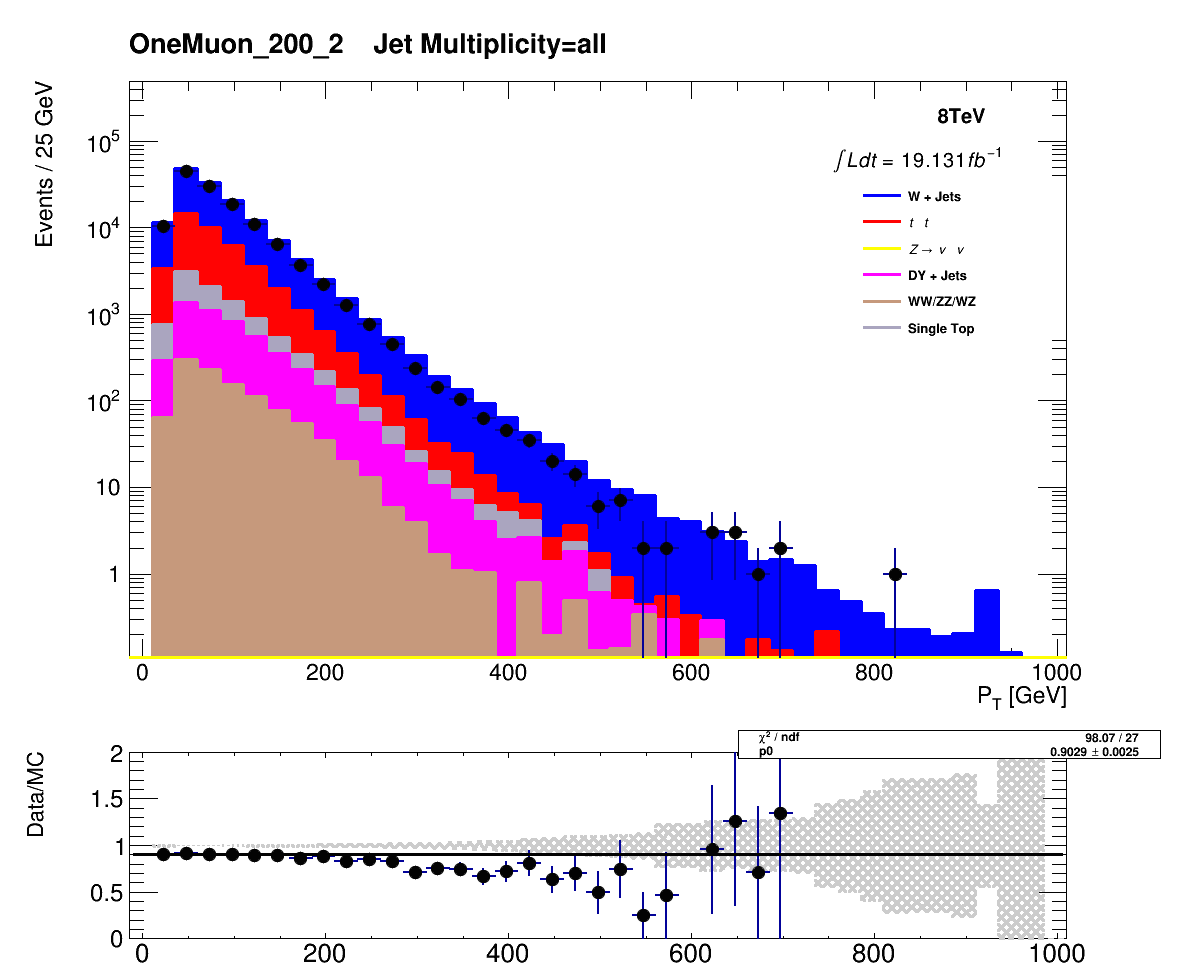
\includegraphics[width=\textwidth]{Figs/datamc/mu/Stacked_MuPt_all_OneMuon_200_upwards}
      \caption{$\mu$ \Pt}
    \end{subfigure}
    \begin{subfigure}[b]{0.48\textwidth}
      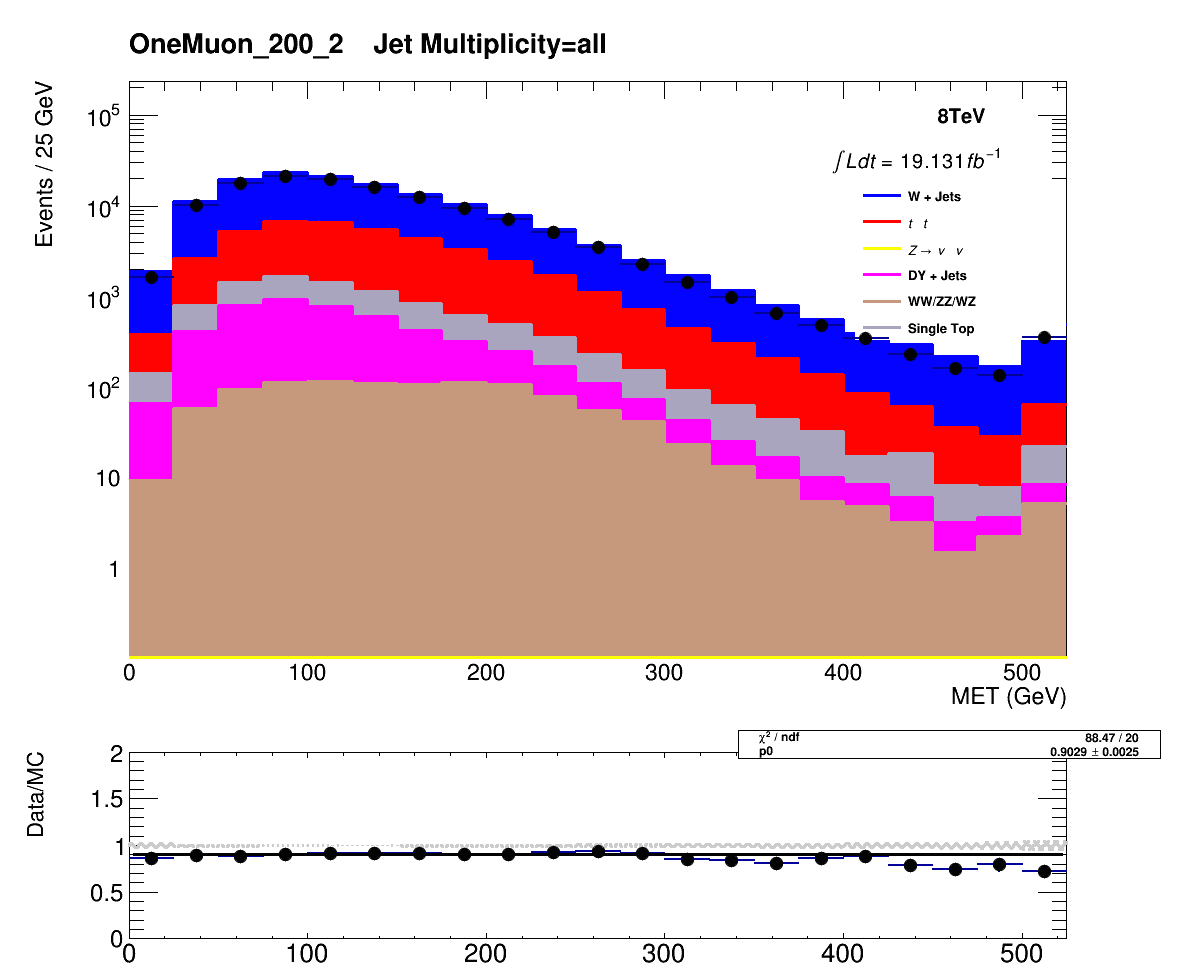
\includegraphics[width=\textwidth]{Figs/datamc/mu/Stacked_MET_Corrected_all_OneMuon_200_upwards}
      \caption{\met (corrected for $\mu$)}
    \end{subfigure} \\
    \caption{\label{fig:datamc_mu_inc}
    Comparison of data with MC for the \mj control selection. Plots 
    are for $\HT>200$~\gev, $\nj\geq2, \nb\geq0$.
    }
\end{figure}

Specifically for the \mj (and \mmj) control samples, no \alphat requirement is
made in order to increase the statistics and therefore the predictive power of 
the samples. This is possible as other requirements, in particular the 
requirement of
a single muon and a specific invariant mass window, greatly reduce any potential
contamination from QCD MJ events. The viability of this is specifically tested 
by dedicated closure tests described later in section~\ref{sec:closure_tests}.

Example distributions of $\mu$ \Pt and $\mu\text{-corrected}$ \met for this selection
are shown in figure~\ref{fig:datamc_mu_inc}.


\subsection{\mmj}
The \mmj sample is constructed to predict background contributions from \zinv 
decays, mimicking this decay via the kinematically similar $Z\to\mu\mu + jets$
process where both muons are subsequently ignored.
The sample is used to provide low \HT coverage for the \zinv background 
prediction, where the \gj sample (section~\ref{sec:gjets_control_sample})
is unable to do so.

\subsubsection{Triggers}
The trigger used is the same as for the \mj sample, as described in
section~\ref{sec:mujets_control_trigger}. Trigger efficiencies are significantly
improved for the dimuon selection given that either of the muons 
can cause a positive trigger decision, as shown in table~\ref{tab:dimuon-trig-effs}. 
Systematic errors are considered of the same magnitude as for the \mj trigger
efficiencies.

% \begin{table}[!ht]
%   \caption{Muon trigger efficiencies (\%) for the \mmj selection listed by
%   \HT bin and \nj category.}
%   \label{tab:dimuon-trig-effs}
%   \centering
%   \small
%   \begin{tabular}{ cccc }
%     \hline
%     \hline
%     \HT (GeV) & 2-3 & $\geq$4 \\ [0.5ex]
                                       
%     \hline
%     150--200  & 98.4 & 98.4  \\
%     200--275  & 98.5 & 98.4  \\
%     275--325  & 98.5 & 98.4  \\
%     325--375  & 98.6 & 98.6  \\
%     375--475  & 98.6 & 98.5  \\
%     475--575  & 98.6 & 98.6  \\
%     575--675  & 98.6 & 98.6  \\
%     675--775  & 98.7 & 98.6  \\
%     775--875  & 98.6 & 98.6  \\
%     875--975  & 98.7 & 98.6  \\
%     975--1075 & 98.7 & 98.8  \\
%     $>$1075   & 98.7 & 98.7  \\
%     \hline
%     \hline
%   \end{tabular}
% \end{table}

\begin{table}[!h]
  \caption{Muon trigger efficiencies (\%) for the \mmj selection listed by \HT bin and
  \nj category.}
  \label{tab:dimuon-trig-effs}
  \centering
  \footnotesize
  \begin{tabular}{ l|cccccccccccc }
    \hline
    \hline
    \multirow{2}{*}{\nj} & \multicolumn{10}{c}{HT bin low edge (GeV)} \\
    & 150 & 200 & 275 & 325 & 375 & 475 & 575 & 675 & 775 & 875 & 975 & 1075 \\
    \hline
    2--3 & 98.4 & 98.5 & 98.5 & 98.6 & 98.6 & 98.6 & 98.6 & 98.7 & 98.6 & 98.7 &
    98.7 & 98.7 \\
    $\geq 4$ & 98.4 & 98.4 & 98.4 & 98.6 & 98.5 & 98.6 & 98.6 & 98.6 & 98.6 & 98.6 & 98.8 &
    98.7 \\
    \hline
  \end{tabular}
\end{table}

\subsubsection{Selection Criteria}

\begin{figure}[t]
  \centering
    \begin{subfigure}[b]{0.48\textwidth}
      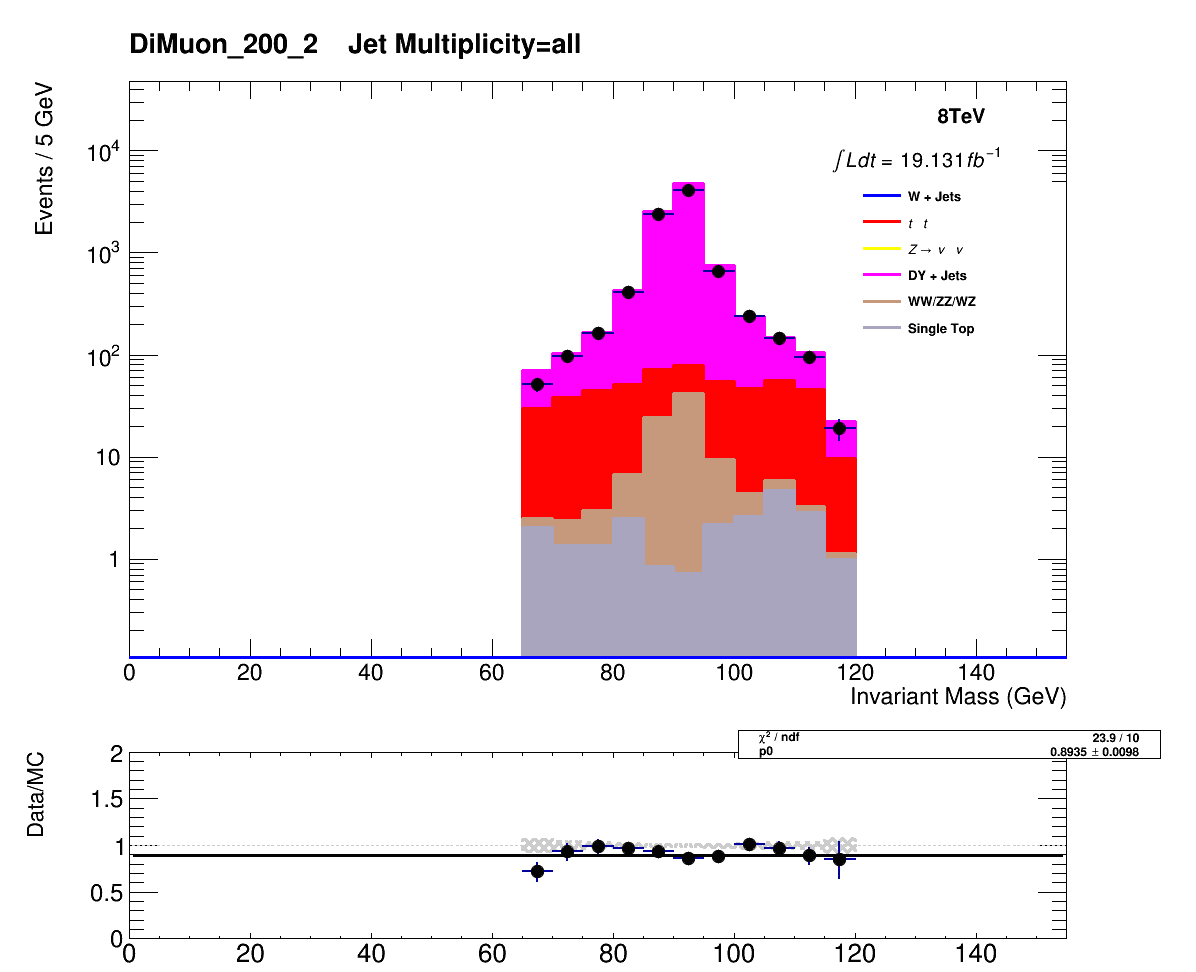
\includegraphics[width=\textwidth]{Figs/datamc/mumu/Stacked_DiMuon_Mass_all_DiMuon_200_upwards}
      \caption{$M_T(\mu, \mu)$}
    \end{subfigure}
    \begin{subfigure}[b]{0.48\textwidth}
      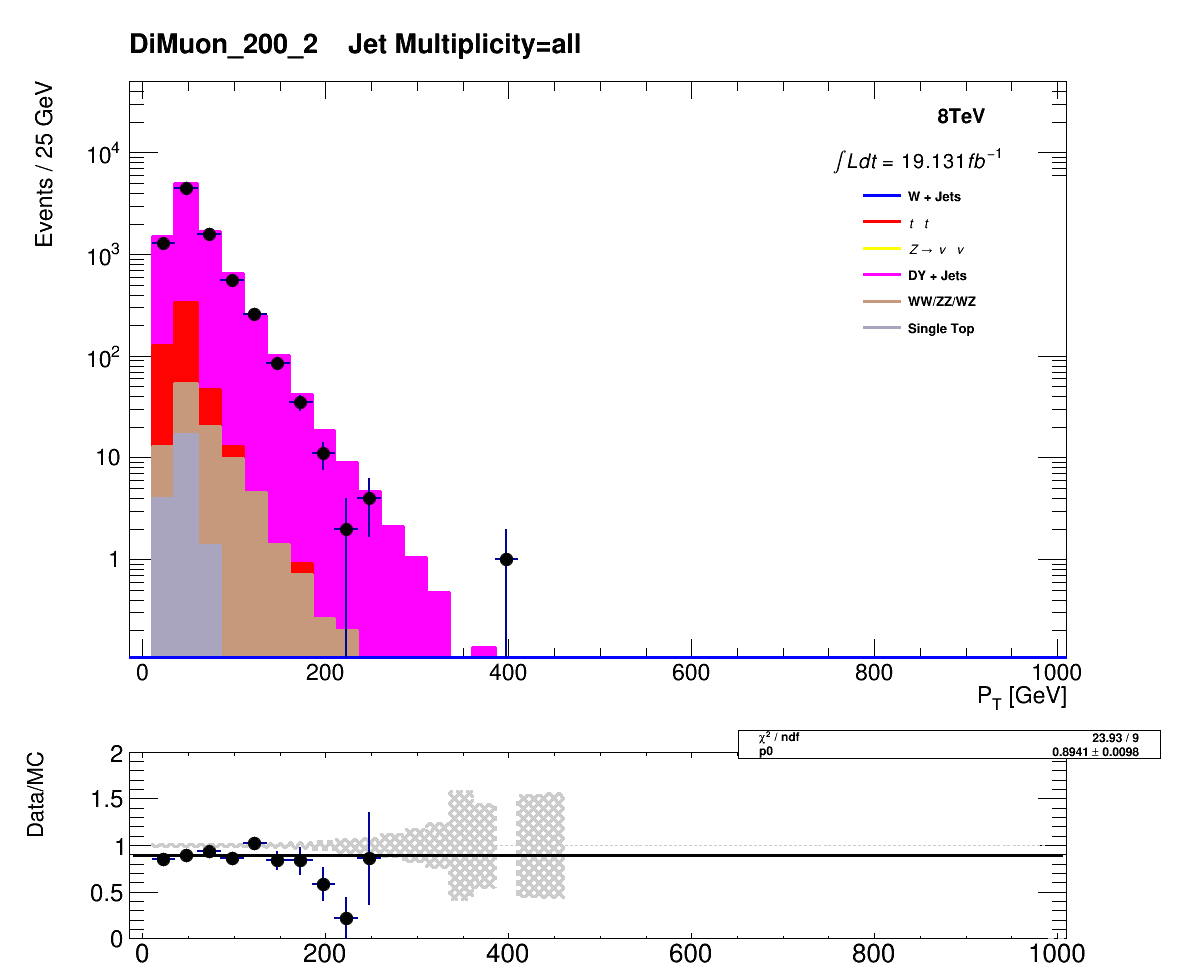
\includegraphics[width=\textwidth]{Figs/datamc/mumu/Stacked_SecondMuPt_all_DiMuon_200_upwards}
      \caption{Second $\mu$ \Pt}
    \end{subfigure} \\
    \caption{\label{fig:datamc_mumu_inc}
    Comparison of data with MC for the \mmj control selection. Plots 
    are for $\HT>200$~\gev, $\nj\geq2, \nb\geq0$.}
\end{figure}

The selection for the \mmj sample is very similar to that of the \mj sample, 
described in section~\ref{sec:mujets_control_selection}, with differences chosen
to enrich the sample in Z bosons decaying to pairs of muons in the kinematic 
phase space of the signal region. Two tight isolated muons are selected, each 
with $\Pt > 30$~\gev and $|\eta| < 2.1$. Their invariant mass is required to be
tight around $m_Z$, $m_Z - 25 < M_{\mu_1\mu_2} < m_Z + 25$~\gev. Furthermore, a 
veto is made on events satisfying $\Delta R(\mu_i, jet_j) < 0.5$, for every muon 
$i$ and every jet $j$. Similarly as in the \mj sample selection, no \alphat
requirement is made.

Example distributions of transverse mass of the muon pair, $M_T(\mu\mu)$, and
$\mu_2$ \Pt for this selection are shown in figure~\ref{fig:datamc_mumu_inc}.

\subsection{\gj}
\label{sec:gjets_control_sample}
The \gj sample is used to predict the \zinv background contribution, given it's 
similar kinematics when the $\gamma$ is ignored from the event, as well as a
larger
production cross section relative to \mmj. Due to trigger thresholds, the \gj
sample cannot make predictions for $\HT<375$~\gev, and so is complimentary to
the \mmj sample prediction.

\subsubsection{Triggers}
Events are collected using the \verb!HLT_Photon150! trigger. The trigger's 
efficiency is measured using the \verb!HLT_Photon90! trigger as a reference and
is found to be 100$\%$ efficient for $E_T^{\gamma}>165$~\gev and $\HT>375$~\gev,

as shown by the turn on curves in figure~\ref{fig:photon_control_trigeff}.

\begin{figure}[t]
  \centering
  \begin{subfigure}[b]{0.35\textwidth}
    \includegraphics[width=\textwidth, page=3,trim=40 40 160 120,clip=true]{figures/trigger/g_barrel_375_caloJet_le3j.pdf}
    \caption{\njlow}
    \label{fig:photon_control_trigeff_le3j}
  \end{subfigure}
  \begin{subfigure}[b]{0.35\textwidth}
    \includegraphics[width=\textwidth, page=3,trim=40 40 160 120,clip=true]{figures/trigger/g_barrel_375_caloJet_ge4j.pdf}
    \caption{\njhigh}
    \label{fig:photon_control_trigeff_ge4j}
  \end{subfigure}
  \caption{Efficiency turn-on curves for the photon trigger, based on the \gj 
  selection, for \HT > 375~\gev, with \njlow (Left) and \njhigh(Right).}
  \label{fig:photon_control_trigeff}
\end{figure}

\subsubsection{Selection Criteria}
Exactly one photon satisfying tight isolation criteria is required, with 
$\Pt > 165$~\gev and $|\eta|<1.45$. In addition, events are vetoed if
$\Delta R(\gamma, jet_i)<1.0$ is satisfied, for all jets $i$ in the event.

An example distribution of the $\gamma$ \Pt for this selection is shown
in figure~\ref{fig:datamc_pho_inc}.

\begin{figure}[!ht]
  \centering
    \begin{subfigure}[b]{0.48\textwidth}
      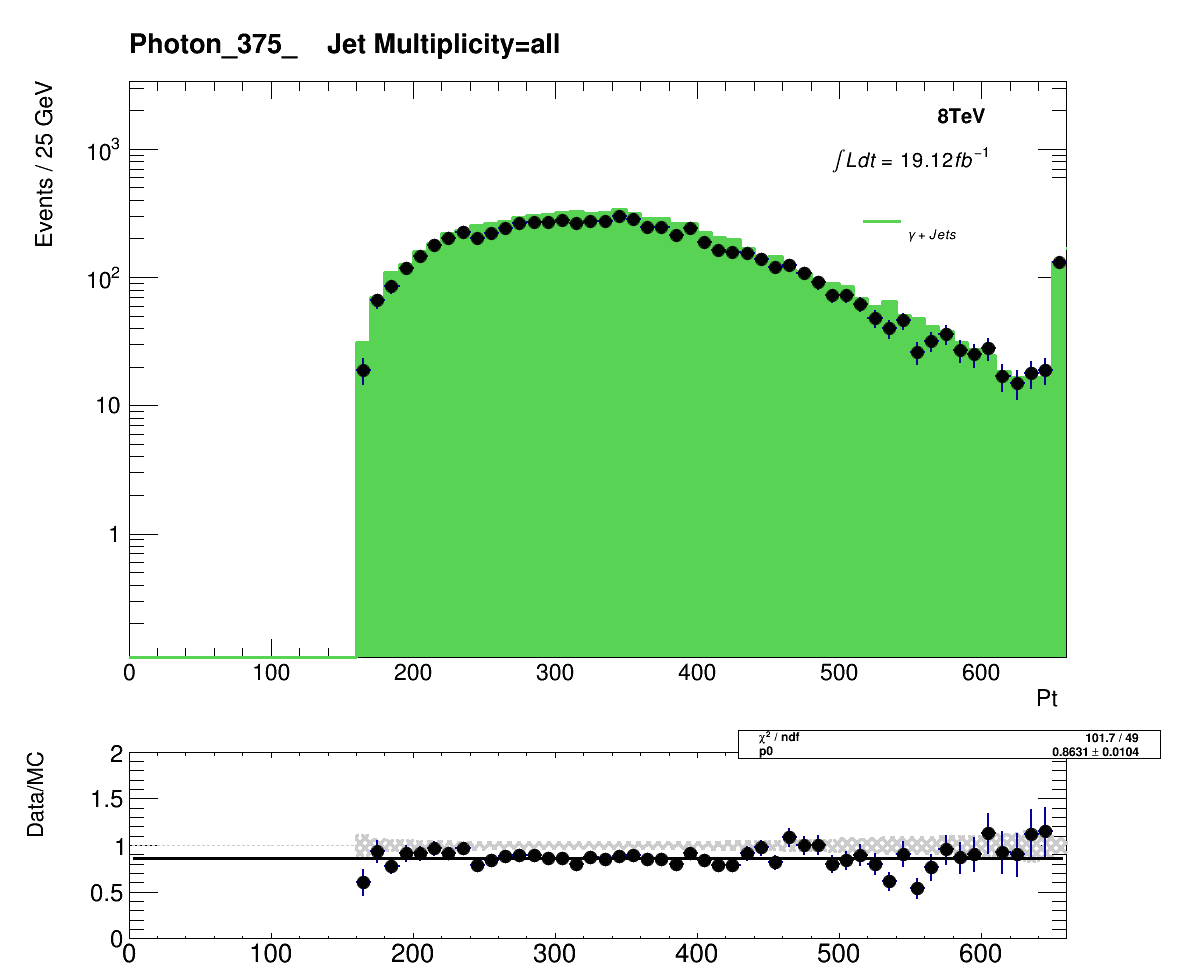
\includegraphics[width=\textwidth]{Figs/datamc/pho/Stacked_PhotonPt_all_Photon_375_upwards}
      \caption{$\gamma$ $\Pt$}
    \end{subfigure}
    \caption{\label{fig:datamc_pho_inc}
    Comparison of data with MC for the \gj control selection. Plot 
    is for $\HT>200$~\gev, $\nj\geq2, \nb\geq0$.}
\end{figure}

%********************************** % Third Section  *************************************
% \section{Estimating multijet backgrounds}  %Section - 1.3
% \label{sec:background_qcd}

% A data-driven technique has been developed to measure any remaining QCD events
% in the signal region. This is used to determine a \HT dependent \alphat
% requirement such that QCD is at the sub-percent level with respect to the total
% EWK background.

% \subsection{Multijet control sample}
% In order to predict the contamination of QCD MJ events in the signal region a 
% control region of hadronic events is constructed.

% \subsubsection{Triggers}
% Events are collected using a suite of triggers requiring various thresholds of 
% \HT. By using single-object \HT triggers it is possible to study events
% across a spectrum of \alphat values. The high rates expected through these
% triggers were maintained throughout
% the 2012 run with a variety of prescales. Each trigger seeds a single \HT bin in
% the analysis, with a 25 \gev offset between the online trigger requirement and 
% the offline threshold. Efficiencies are measured with the same technique as the
% signal triggers, using the \verb!HLT_IsoMu24_eta2p1! trigger as a reference. 
% The efficiencies of these triggers are summarised in table~\ref{tab:ht-triggers}.

% \begin{table}[!ht]
%   \caption{List of \texttt{HTxxx} triggers and their efficiencies
%     (\%), as measured in data for each \HT bin and \nj category. Also listed are
%     the typical prescales applied and the L1 seed triggers.}
%   \label{tab:ht-triggers}
%   \centering
%   \scriptsize
%   \begin{tabular}{ ccccll }
%     \hline
%     \hline
%     Offline \HT & L1 seed (\verb!L1_?!) & Trigger (\verb!HLT_?!) &    Typical & \multicolumn{2}{c}{Efficiency (\%)}\\ [0.5ex]
%    region (\gev) & (highest thresholds) &  & prescale & \multicolumn{1}{c}{$2 \leq \nj \leq 3$} & \multicolumn{1}{c}{$\nj \geq 4$} \\ [0.5ex]

%     \hline
%     $200 < \HT < 275$  & \verb!DoubleJetC64!           & \verb!HT250! & 4800     & $\phantom{1}66.4 \pm 14.1$                & $154.3 \pm 154.3$                     \\
%     $275 < \HT < 325$  & \verb!DoubleJetC64 OR HTT175! & \verb!HT250! & 2400     & $\phantom{1}97.3 \pm 23.0$                & $\phantom{1}91.7 \pm \phantom{1}53.1$ \\
%     $325 < \HT < 375$  & \verb!DoubleJetC64 OR HTT175! & \verb!HT300! & 1200     & $\phantom{1}79.5 \pm 20.6$                & $198.1 \pm \phantom{1}81.2$           \\
%     $375 < \HT < 475$  & \verb!DoubleJetC64 OR HTT175! & \verb!HT350! & 600      & $108.7 \pm 18.7$                          & $\phantom{1}54.5 \pm \phantom{1}31.6$ \\
%     $475 < \HT < 575$  & \verb!DoubleJetC64 OR HTT175! & \verb!HT450! & 150      & $110.6 \pm 15.9$                          & $106.4 \pm \phantom{1}26.8$           \\
%     $575 < \HT < 675$  & \verb!DoubleJetC64 OR HTT175! & \verb!HT550! & 70       & $\phantom{1}96.1 \pm 14.7$                & $104.4 \pm \phantom{1}23.1$           \\
%     $675 < \HT < 775$  & \verb!DoubleJetC64 OR HTT175! & \verb!HT650! & 25       & $\phantom{1}94.3 \pm 15.4$                & $101.2 \pm \phantom{1}21.5$           \\
%     $775 < \HT < 875$  & \verb!DoubleJetC64 OR HTT175! & \verb!HT750! & 1        & $\phantom{1}96.9 \pm \phantom{1}6.1$      & $\phantom{1}94.4 \pm \phantom{11}8.3$ \\
%     $875 < \HT < 975$  & \verb!DoubleJetC64 OR HTT175! & \verb!HT750! & 1        & $100.0 \pm \phantom{1}8.4$                & $100.0 \pm \phantom{1}12.6$           \\
%     $975 < \HT < 1075$ & \verb!DoubleJetC64 OR HTT175! & \verb!HT750! & 1        & $100.0 \pm 11.2$                          & $100.0 \pm \phantom{1}15.3$           \\
%     $\HT > 1075$       & \verb!DoubleJetC64 OR HTT175! & \verb!HT750! & 1        & $100.0 \pm 15.0$                          & $100.0 \pm \phantom{1}22.9$           \\
%     \hline
%     \hline
%   \end{tabular}
% \end{table}

% \subsubsection{Selection Criteria}
% The selection of this sample matches that of the hadronic signal region, with 
% the exception that both the \alphat and \mhtmet requirements are removed 
% ensuring a very high yield of QCD MJ events.


% \subsection{Prediction Technique}

% Events from the hadronic control sample are used to populate a plane of \mhtmet 
% and \alphat. A prediction of the EWK contribution to this sample is determined 
% from the \mj control sample with the \mhtmet requirement removed, using the TF 
% factor method described in section~\ref{sec:background_overview}. The prediction
% is subtracted from the hadronic control sample yields as a function of \mhtmet
% and \alphat, leaving a pure sample of QCD MJ events (SHOW PLOTS?).

% By considering events both above and below the nominal \mhtmet threshold of
% 1.25, the ratio \rmhtmet is constructed, defined as:
% % 
% \begin{equation}
% \label{eq:rmhtmet}
% \rmhtmet = \frac{N(\mhtmet<1.25)}{N(\mhtmet>1.25)}
% \end{equation}

% A fit is made to this variable as a function of \alphat, using an exponential 
% functional form:
% % 
% \begin{equation}
% \label{eq:fit_exp}
% \rmhtmet(\alphat) = e^{{-(a+b.\alphat)}^n}
% \end{equation}
% % 
% both for $n=0$ and also when $n$ is allowed to float as a free 
% parameter within the range $0-2$ in order to span the scenarios from flat to a
% Gaussian form. Example distributions and fits are shown in FIGURE.

% QCD yield predictions are made and compared with the relevant EWK background 
% contributions in table~\ref{tab:qcd-pred-data}. \alphat thresholds are chosen 
% for each \HT bin such that the ratio of QCD to EWK is at the sub-percent level. 
% The chosen \alphat threshold values are summarised in
% table~\ref{tab:alphat_thresholds_qcd}.

% \begin{table}[h!]
% \centering
% \scriptsize
%   \caption{QCD multijet background contribution prediction summarised for the 
%   main analysis categories of \nb, \nj and \HT as a function of \alphat. The 
%   predicted EWK background contribution is included for comparison, and a 
%   the ratio of QCD/EWK is also shown.}
% \label{tab:qcd-pred-data}
% \begin{tabular}{ccccrrr}
% \hline
% \hline
% \nj & \nb & \HT (GeV) & Bkgd & \multicolumn{3}{c}{\alphat threshold} \\
% \cline{5-7}
%  & & & & \multicolumn{1}{c}{0.550}   & \multicolumn{1}{c}{0.600}   & \multicolumn{1}{c}{0.650} \\
% \hline
% 2--3 & 0 & 200--275 & QCD  & $\left(3.8 \pm 1.3 \pm 1.2 \right) \times 10^{3}$ & $\left(4.1 \pm 2.4 \pm 3.0 \right) \times 10^{1}$ & $\left(0.9 \pm 0.8 \pm 1.5 \right) \times 10^{0}$\\
% 2--3 & 0 & 200--275 & EWK  & $\left(2.1 \pm 0.1\right) \times 10^{4}$ & $\left(1.5 \pm 0.0\right) \times 10^{4}$ & $\left(1.2 \pm 0.0\right) \times 10^{4}$\\
% 2--3 & 0 & 200--275 & Ratio  & $0.2 \pm 0.1$ & $0.003 \pm 0.003$ & $0.0001 \pm 0.0001$\\ [1.0ex]
% 2--3 & 0 & 275--325 & QCD  & $\left(1.0 \pm 0.3 \pm 1.5 \right) \times 10^{4}$ & $\left(0.2 \pm 0.1 \pm 0.7 \right) \times 10^{0}$ & $\left(0.8 \pm 0.3 \pm 4.8 \right) \times 10^{-3}$\\
% 2--3 & 0 & 275--325 & EWK  & $\left(7.9 \pm 0.2\right) \times 10^{3}$ & $\left(5.3 \pm 0.2\right) \times 10^{3}$ & $\left(4.0 \pm 0.2\right) \times 10^{3}$\\
% 2--3 & 0 & 275--325 & Ratio  & $1 \pm 2$ & $0.0000 \pm 0.0001$ & $\left(0 \pm 1\right) \times 10^{-6}$\\ [1.0ex]
% 2--3 & 0 & 325--375 & QCD  & $\left(2.8 \pm 0.4 \pm 2.1 \right) \times 10^{1}$ & $\left(0.9 \pm 0.2 \pm 1.3 \right) \times 10^{-1}$ & $\left(0.6 \pm 0.4 \pm 1.2 \right) \times 10^{-3}$\\
% 2--3 & 0 & 325--375 & EWK  & $\left(3.4 \pm 0.1\right) \times 10^{3}$ & $\left(2.2 \pm 0.1\right) \times 10^{3}$ & $\left(1.7 \pm 0.1\right) \times 10^{3}$\\
% 2--3 & 0 & 325--375 & Ratio  & $0.008 \pm 0.006$ & $\left(4 \pm 6\right) \times 10^{-5}$ & $\left(4 \pm 8\right) \times 10^{-7}$\\ [1.0ex]
% $\geq 4$ & 0 & 200--275 & QCD  & $\left(2.8 \pm 1.5 \pm 1.3 \right) \times 10^{3}$ & $\left(1.1 \pm 0.7 \pm 0.2 \right) \times 10^{1}$ & $\left(0.2 \pm 0.2 \pm 0.0 \right) \times 10^{0}$\\
% $\geq 4$ & 0 & 200--275 & EWK  & $\left(4.3 \pm 0.3\right) \times 10^{2}$ & $\left(2.0 \pm 0.1\right) \times 10^{2}$ & $\left(1.0 \pm 0.1\right) \times 10^{2}$\\
% $\geq 4$ & 0 & 200--275 & Ratio  & $7 \pm 5$ & $0.06 \pm 0.04$ & $0.002 \pm 0.002$\\ [1.0ex]
% $\geq 4$ & 0 & 275--325 & QCD  & $\left(1.5 \pm 1.2 \pm 1.0 \right) \times 10^{4}$ & $\left(1.5 \pm 1.7 \pm 0.3 \right) \times 10^{0}$ & $\left(0.1 \pm 0.2 \pm 0.0 \right) \times 10^{-1}$\\
% $\geq 4$ & 0 & 275--325 & EWK  & $\left(1.2 \pm 0.0\right) \times 10^{3}$ & $\left(5.3 \pm 0.2\right) \times 10^{2}$ & $\left(2.9 \pm 0.1\right) \times 10^{2}$\\
% $\geq 4$ & 0 & 275--325 & Ratio  & $\left(1 \pm 1\right) \times 10^{1}$ & $0.003 \pm 0.003$ & $\left(4 \pm 7\right) \times 10^{-5}$\\ [1.0ex]
% $\geq 4$ & 0 & 325--375 & QCD  & $\left(0.7 \pm 0.1 \pm 0.8 \right) \times 10^{0}$ & $\left(2.5 \pm 0.6 \pm 6.5 \right) \times 10^{-5}$ & $\left(0.7 \pm 0.3 \pm 2.8 \right) \times 10^{-8}$\\
% $\geq 4$ & 0 & 325--375 & EWK  & $\left(4.8 \pm 0.3\right) \times 10^{2}$ & $\left(2.0 \pm 0.1\right) \times 10^{2}$ & $\left(1.1 \pm 0.1\right) \times 10^{2}$\\
% $\geq 4$ & 0 & 325--375 & Ratio  & $0.002 \pm 0.002$ & $\left(1 \pm 3\right) \times 10^{-7}$ & $\left(1 \pm 3\right) \times 10^{-10}$\\ [1.0ex]
% %2--3 & $\geq 1$ & 200--275 & QCD  & $\left(2.2 \pm 1.1 \pm 4.5 \right) \times 10^{2}$ & $\left(0.5 \pm 0.2 \pm 3.2 \right) \times 10^{0}$ & $\left(0.3 \pm 0.1 \pm 4.5 \right) \times 10^{-2}$\\
% %2--3 & $\geq 1$ & 200--275 & EWK  & $\left(3.7 \pm 0.1\right) \times 10^{3}$ & $\left(2.5 \pm 0.1\right) \times 10^{3}$ & $\left(1.9 \pm 0.1\right) \times 10^{3}$\\
% %2--3 & $\geq 1$ & 200--275 & Ratio  & $0.1 \pm 0.1$ & $0.000 \pm 0.001$ & $\left(0 \pm 2\right) \times 10^{-5}$\\ [1.0ex]
% \hline
% \hline
% \end{tabular}
% \end{table}

% \emph{RELATED SYSTEMATICS?}

% \begin{table}[!ht]
%   \caption{\alphat thresholds for each analysis \HT bin as determined from the 
%   QCD MJ prediction method, such that QCD is at the sub-percent level.}
%   \label{tab:alphat_thresholds_qcd}
%   \centering
%   \small
%   \begin{tabular}{ cc }
%     \hline
%     \hline
%     \HT (GeV) & \alphat threshold \\ [0.5ex]
                                       
%     \hline
%     200--275  & 0.65 \\
%     275--325  & 0.60 \\
%     >325  & 0.55 \\
%     \hline
%     \hline
%   \end{tabular}
% \end{table}


%********************************** % Fifth Section  *************************************
\section{Systematic uncertainties on SM background predictions}  %Section - 1.5
\label{sec:background_systematics}

In order to probe the levels at which the transfer factors are sensitive to 
relevant uncertainties, a statistically powerful ensemble of Closure Tests
(CT's) have been designed. The CT method works by constructing a TF to
extrapolate from one sub-region of a particular control sample into another 
control sample sub-region. In doing so, tests can be designed to specifically 
probe any potential sources of bias in the transfer factors.

\subsection{Closure tests}
\label{sec:closure_tests}

Closure tests are performed as a function of \HT, in the two \nj categories,
\njlow and \njhigh. The level of closure is represented by the statistical 
consistency between predicted and observed yields for each test, in the absence 
of any assumed systematic uncertainty. The test statistic is defined as $(N_{obs}
- N_{pred}) / N_{pred}$, with any bias being observed as a statistically 
significant deviation from zero, or trend in \HT.

\begin{figure}[ht!]
  \centering
  \begin{subfigure}[b]{0.7\textwidth}
    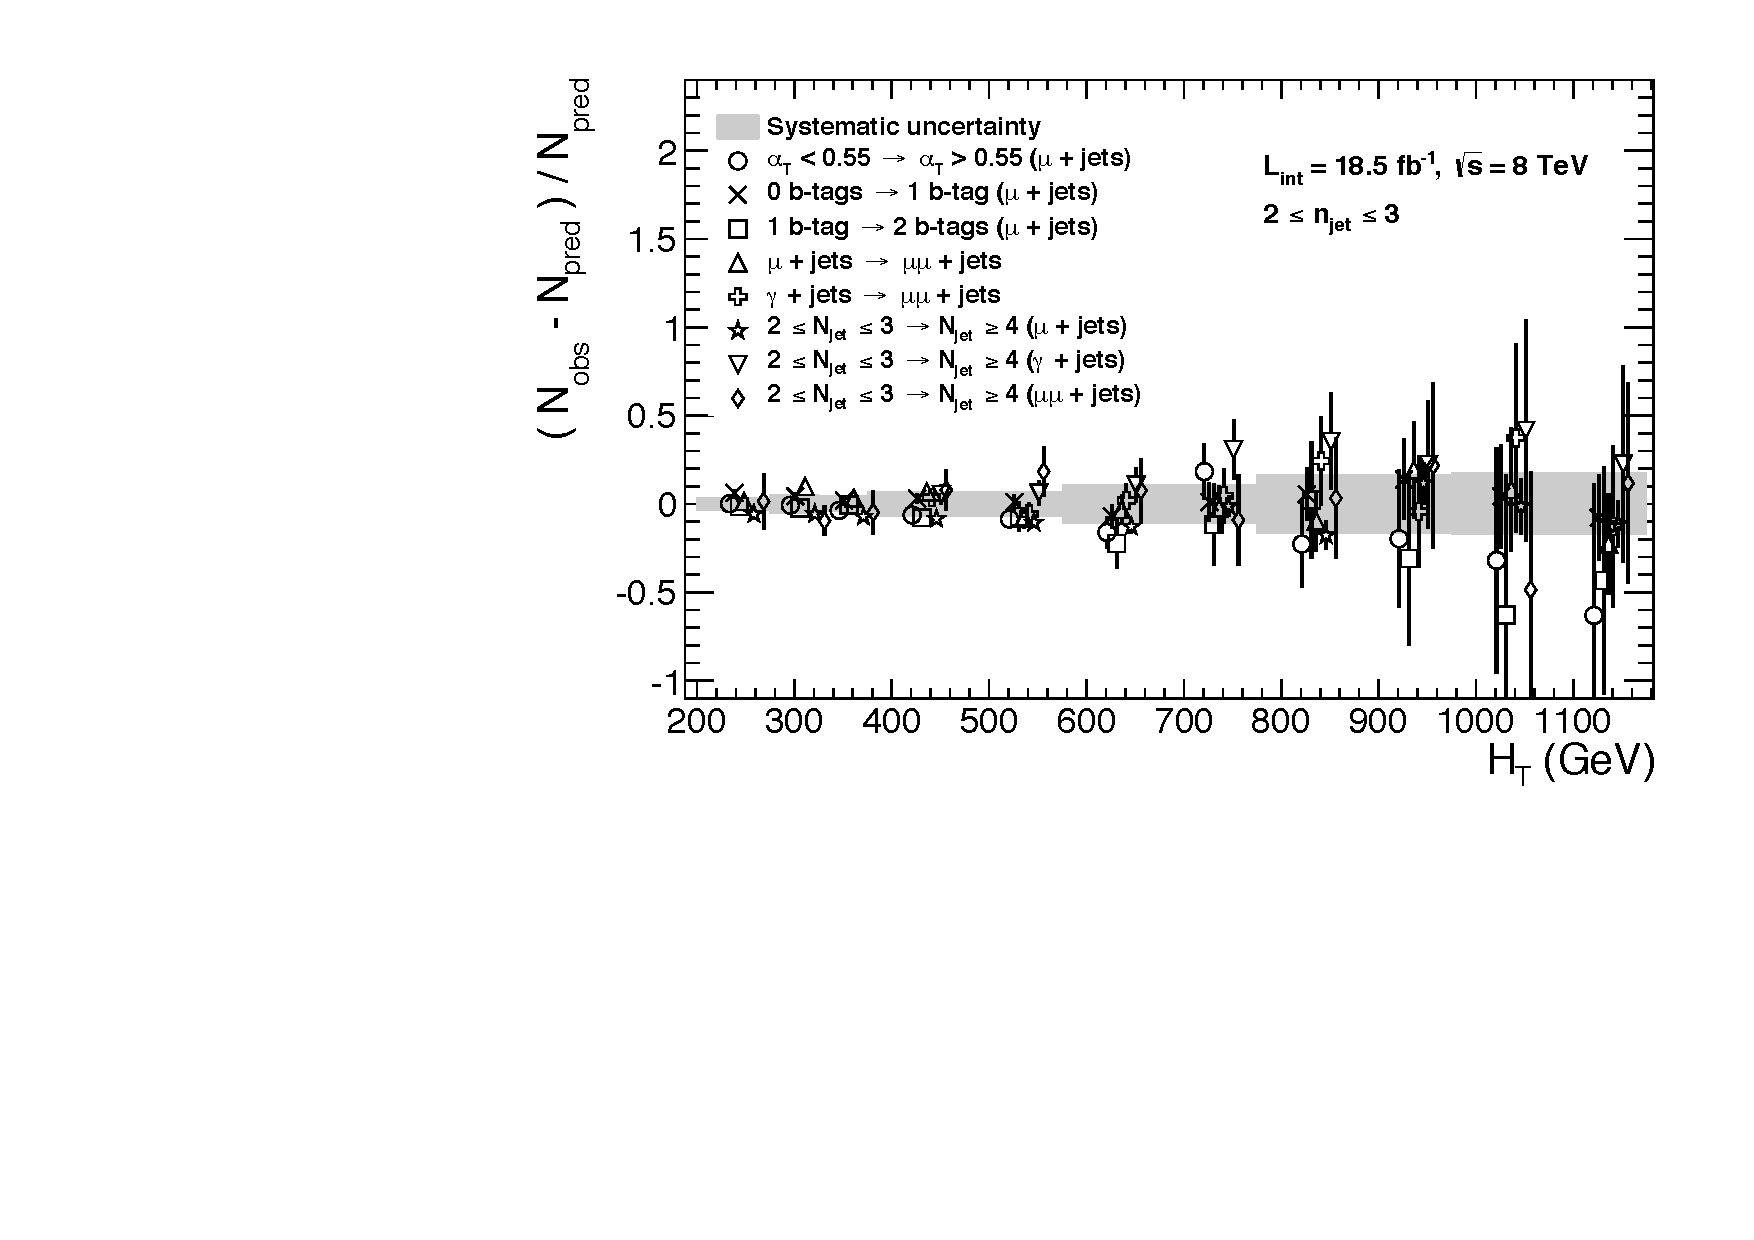
\includegraphics[width=\textwidth]{Figs/syst/v0/le3j/summary_plot}
    \caption{$2 \leq \nj \leq 3$}
    \label{fig:closure_summary_le3j}
  \end{subfigure}             
  \begin{subfigure}[b]{0.7\textwidth}
    \includegraphics[width=\textwidth]{Figs/syst/v0/ge4j/summary_plot}
    \caption{$\nj \geq 4$}
    \label{fig:closure_summary_ge4j}
  \end{subfigure}
  \caption{The results of the eight core closure tests (open symbols), shown 
  over the systematic uncertainty bands for each of the five \HT regions
  (shaded grey), for the two jet multiplicity regions (a) \njlow and (b) \njhigh.}
  \label{fig:closure_summary}
\end{figure}

Figure~\ref{fig:closure_summary} shows a summary of the eight closure tests 
considered as `core' tests for the analysis, split into both
\njlow (figure~\ref{fig:closure_summary_le3j}) 
and \njhigh (figure~\ref{fig:closure_summary_ge4j}). It should be noted that 
numerous other tests are also considered, but that these eight represent those 
deemed most important to the background prediction and are therefore used to
derive related uncertainties.

The first test, represented by open circles, tests the modelling of the \alphat 
variable in the \mj control sample. In the analysis a prediction is made 
between the \mj sample, which has no \alphat requirement, and the 
signal region, with it's tight \alphat requirement. This particular test probes
the validity of the prediction between the `bulk' of the \alphat distribution in
the control sample
and the `tail' of the distribution in the signal region. A similar test, not
shown here, is performed for the \mmj control sample.

The next two tests, represented by crosses and open squares, probe the
different b tag multiplicities in the \mj control sample. The b tag 
requirements greatly change the relative admixture of, for example, \wj (\nb=0)
and \ttj (\nb=1) events.
It is important to note that this test is 
considered conservative, given that the admixture of \wj to \ttj events 
varies minimally between control and signal regions, where this extrapolation is 
made between identical \nb categories in the analysis. Given the focus on b
tagging, these tests also investigate the modelling of b quark jets in the
simulated data.

Represented by open triangles, a similar test is made for the relative
admixture of \zj to \wj and \ttj, by  predicting between the \mj and \mmj
control regions. Again, this test is considered conservative, and also probes
the muon reconstruction and trigger efficiencies between the different muon
multiplicities. These are however already well studied by the muon \emph{POG}
using data-driven techniques.

As described in section~\ref{sec:background_overview}, the \zinv prediction 
is made from both the \gj and \mmj samples, and so a test is constructed to 
predict between these two orthogonal control regions, as shown by the open 
crosses.

The final three tests, indicated by open stars, triangles and diamonds, make 
predictions between the two different jet multiplicity categories in each 
control sample, thereby 
testing jet reconstruction and modelling. These tests are also considered 
conservative as the analysis only predicts between identical \nj categories in 
the control and signal regions.

Summary plots of these eight tests are shown in
figure~\ref{fig:closure_summary}, indicating no statistically significant biases
or \HT dependencies. Figures~\ref{fig:closure_fit_le3j_pol0} and \ref{fig:closure_fit_ge4j_pol0} show
zeroeth order polynomial fits (blue lines) made to each individual test to assess the 
level of any potential bias present. In addition, first order polynomial fits 
(red lines) are made to assess any potential \HT dependence present in the
tests, as shown
in figures~\ref{fig:closure_fit_le3j_pol1} and \ref{fig:closure_fit_ge4j_pol1}.
The best-fit values, $\chi^2$ and $p$-values 
obtained from both fits are summarised for each \nj category in
tables~\ref{tab:syst-fits-le3j}, \ref{tab:syst-fits-ge4j} and
\ref{tab:syst-fits-njet}.

The fits show no significant biases or trends and therefore indicate good
closure. The only exception is the 0 b-jets \ra 1 b-jet (\mj) test for the
\njhigh category which has a sub-optimal goodness of fit value. This is 
attributed to upwards and downwards fluctuations in the adjacent 475-575~\gev
and 575-675~\gev bins respectively. Also shown in table~\ref{tab:syst-fits-ge4j},
when the same fit is made after summing these two bins significantly improved
fit parameters are observed. This leads to the conclusion that these two
bins contain a statistical fluctuation as opposed to a systematic bias.

\begin{figure}[ht!]
  \centering
  \begin{subfigure}[b]{0.46\textwidth}
    \includegraphics[width=\textwidth]{figures/syst/v0/le3j/summary_plot_pol0}
    \caption{$2 \leq \nj \leq 3$ (constant function fits)}
    \label{fig:closure_fit_le3j_pol0}
  \end{subfigure}
  \begin{subfigure}[b]{0.46\textwidth}
    \includegraphics[width=\textwidth]{figures/syst/v0/le3j/summary_plot_pol1}
    \caption{$2 \leq \nj \leq 3$ (linear function fits)}
    \label{fig:closure_fit_le3j_pol1}
  \end{subfigure}
  \begin{subfigure}[b]{0.46\textwidth}
    \includegraphics[width=\textwidth]{figures/syst/v0/ge4j/summary_plot_pol0}
    \caption{$\nj \geq 4$ (constant function fits)}
    \label{fig:closure_fit_ge4j_pol0}
  \end{subfigure}
  \begin{subfigure}[b]{0.46\textwidth}
    \includegraphics[width=\textwidth]{figures/syst/v0/ge4j/summary_plot_pol1}
    \caption{$\nj \geq 4$ (linear function fits)}
    \label{fig:closure_fit_ge4j_pol1}
  \end{subfigure}
  \caption{The results of the eight core closure tests (open symbols), shown 
  over the systematic uncertainty bands for each of the five \HT regions
  (shaded grey), for the two jet multiplicity regions (a) \njlow and (b) \njhigh 
  separately. Included are zeroeth order (left column, blue) and first order
  (right column, red) fits to each individual closure test.}
  \label{fig:closure_fits}
\end{figure}

\begin{table}[!ht]
  \caption{Results of zeroeth (i.e. constant) and first order (i.e. linear) fits
  for five sets of closure tests, performed in the \njlow category.}
  \label{tab:syst-fits-le3j}
  \centering
  \tiny
  \begin{tabular}{ llrccccrc }
    \hline
    \hline
                                              &          & \multicolumn{4}{c}{Constant fit} &          & \multicolumn{2}{c}{Linear fit}                        \\
    \cline{3-6}\cline{8-9}                                                                  
    Closure test                              & Symbol   & Best fit value                   & $\chi^2$ & d.o.f. & $p$-value &  & Slope ($10^{-4}$) & $p$-value \\
    \hline                                                                                                                                  
    $\alphat < 0.55 \ra \alphat > 0.55$ (\mj) & Circle   & $-0.02 \pm 0.01$                 & 11.3     & 10     & 0.34      &  & $-2.9 \pm 1.1$    & 0.83      \\ 
    0 b-jets \ra 1 b-jet (\mj)                & Times    & $ 0.04 \pm 0.01$                 & 5.8      & 10     & 0.83      &  & $-1.5 \pm 0.9$    & 0.97      \\ 
    1 b-jet \ra 2 b-jets (\mj)                & Square   & $-0.03 \pm 0.02$                 & 5.3      & 10     & 0.87      &  & $-3.0 \pm 1.7$    & 0.99      \\ 
    \mj \ra \mmj                              & Triangle & $ 0.03 \pm 0.02$                 & 12.3     & 10     & 0.27      &  & $-1.3 \pm 1.1$    & 0.28      \\ 
    \gj \ra \mmj                              & Cross    & $-0.02 \pm 0.03$                 & 3.0      & 7      & 0.88      &  & $ 0.0 \pm 2.7$    & 0.81      \\ 
    \hline
    \hline
  \end{tabular}
\end{table}

\begin{table}[!ht]
  \caption{Results of zeroeth (i.e. constant) and first order (i.e. linear) fits
  for five sets of closure tests, performed in the \njlow category. An
  additional test marked with a $\dag$ is listed, as described in the text.}
  \label{tab:syst-fits-ge4j}
  \centering
  \tiny
  \begin{tabular}{ llrccccrc }
    \hline
    \hline
                                              &          & \multicolumn{4}{c}{Constant fit} &          & \multicolumn{2}{c}{Linear fit}                        \\
    \cline{3-6}\cline{8-9}                                                                  
    Closure test                              & Symbol   & Best fit value                   & $\chi^2$ & d.o.f. & $p$-value &  & Slope ($10^{-4}$) & $p$-value \\
    \hline                                                                                                                                 
    $\alphat < 0.55 \ra \alphat > 0.55$ (\mj) & Circle   & $-0.02 \pm    0.02$              & 17.6     & 10     & 0.06      &  & $-3.1 \pm 1.7$    & 0.11      \\ 
    0 b-jets \ra 1 b-jet (\mj)                & Times    & $-0.06 \pm 0.02$                 & 31.2     & 10     & 0.00      &  & $-4.1 \pm 1.2$    & 0.02      \\ 
    0 b-jets \ra 1 b-jet (\mj)$^{ \dag}$      & Times    & $-0.05 \pm 0.02$                 & 13.4     & 9      & 0.15      &  & $-3.9 \pm 1.3$    & 0.78      \\ 
    1 b-jet \ra 2 b-jets (\mj)                & Square   & $ 0.06 \pm    0.02$              & 13.7     & 10     & 0.19      &  & $ 2.5 \pm 1.6$    & 0.28      \\ 
    \mj \ra \mmj                              & Triangle & $ 0.11 \pm    0.05$              & 4.8      & 10     & 0.90      &  & $ 0.4 \pm 2.7$    & 0.85      \\ 
    \gj \ra \mmj                              & Cross    & $-0.00 \pm 0.07$                 & 2.3      & 7      & 0.94      &  & $-5.3 \pm 4.7$    & 0.99      \\ 
    \hline
    \hline
  \end{tabular}
\end{table}

\begin{table}[!ht]
  \caption{Results of zeroeth (i.e. constant) and first order (i.e. linear) fits
  for the three sets of closure tests probing the accuracy of jet multiplicity 
  modelling in MC, for each control sample.} 
  \label{tab:syst-fits-njet}
  \centering
  \footnotesize
  \begin{tabular}{ llrccccrc }
    \hline
    \hline
           &                   & \multicolumn{4}{c}{Constant fit} &          & \multicolumn{2}{c}{Linear fit}                        \\
    \cline{3-6}\cline{8-9}
    Sample & Symbol            & Best fit value                   & $\chi^2$ & d.o.f. & $p$-value &  & Slope ($10^{-4}$) & $p$-value \\
    \hline                                                                                                            
    \mj    & Star              & $-0.08 \pm 0.01$                 & 9.3      & 10     & 0.50      &  & $0.6 \pm 0.7$     & 0.48      \\ 
    \gj    & Inverted triangle & $ 0.09 \pm 0.04$                 & 3.7      & 7      & 0.82      &  & $5.1 \pm 3.2$     & 0.98      \\ 
    \mmj   & Diamond           & $-0.00 \pm 0.05$                 & 4.7      & 10     & 0.91      &  & $2.5 \pm 2.9$     & 0.92      \\ 
    \hline
    \hline
  \end{tabular}
\end{table}

\subsection{Background systematic uncertainty summary}
Under the assumption of closure for the eight core tests,
systematic errors are derived for each \nj category in seven regions of \HT.
Values are calculated by summing in quadrature the weighted mean and sample 
variance for all eight tests in a given \HT region. These values are summarised 
in table~\ref{tab:syst_values} and also in the summary plots of figure~\ref{fig:closure_summary},
shown as grey bands.

\begin{table}[!ht]
  \caption{Summary of the magnitude of systematic uncertainties (\%) derived 
  from the eight core closure tests, for each \nj category and \HT region.}
  \label{tab:syst_values}
  \centering
  \footnotesize
  \begin{tabular}{ cccccccc }
    \hline
    \hline
            & \multicolumn{7}{c}{\HT region (GeV)}                                \\
    \cline{2-8}
    \nj   & 200--275 & 275--325 & 325--375 & 375--575 & 575--775 & 775-975 & $>975$ \\
    \hline                                                                                                                                  
    2--3    & 4        & 6        & 6        & 8        & 12       & 17      & 19     \\
    $\geq$4 & 6        & 6        & 11       & 11       & 18       & 20      & 26     \\
    \hline                                                                                                                                  
    \hline
  \end{tabular}
\end{table}

Systematic values are considered as fully uncorrelated between the 
different analysis categories and the \HT regions, which is again 
considered as a conservative approach given that some correlation is to be 
expected, for example between adjacent \HT bins.

%********************************** % blah Section  *************************************

\section{QCD control}
\label{sec:qcd_cleaning}

While the \alphat requirement removes many orders of magnitude of QCD events,
there still exist scenarios in which these events may pass the signal region
selection. Accordingly, further requirements are made to ensure the search
region is free of any residual QCD contamination.

\subsection{Multiple jets below threshold}
\label{sec:qcd_cleaning_below_thresh}

Events are able to acquire non-negligible amounts of \mht without the presence
of
real \met if multiple jets are below the jet \Pt threshold and their
configuration conspires to form a topology that gives high values of \alphat.
Such events will contain a disparity between the \met and
\mht variables, given that the former is reconstructed using energy deposits
and the latter with reconstructed jet objects.
Figure~\ref{fig:full_mhtmet_distro} shows the significant contribution of QCD at
high \mhtmet values, even following the \alphat requirement.
To protect against this scenario, events are required to have \mhtmet < 1.25.

\begin{figure}[t]
\centering
\includegraphics[width=0.6\textwidth]
{Figs/datamc/had/v1/Stacked_MHTovMET_all_200_upwards.png}
\caption{The \mhtmet distribution of MC events following the hadronic selection
criteria, minus the nominal \mhtmet requirement.The MC yields are stacked,
with the QCD contribution shown in cyan. The plot is for a fully inclusive
selection of $\nb \geq 0$, $\nj \geq 2$ and \HT > 200~\gev.}
\label{fig:full_mhtmet_distro}
\end{figure}

\subsection{Instrumental effects}

Fake \mht may also be produced if jets overlap with areas of the calorimeter 
system which are damaged or known to be faulty (hereby referred to as `dead'),
and jets are mismeasured or lost as a result. To protect against this, for a
given jet $j$ the angular separation between the event \mht, calculated
excluding jet $j$, and the jet itself is defined as:
% 
\begin{equation}
\dphistar_j = \Delta \phi\big(\overrightarrow{\Pt}_j,-\sum_{i\neq j}
{\overrightarrow{\Pt}_i}\big) .
\label{eq:biasdphi}
\end{equation}
% 
An advantage of this variable with respect to the often used
$\Delta R(\overrightarrow{\Pt}_j, \mht)$ is it's detection of spurious missing
energy vectors
caused
by both under-measurements and over-measurements of a jet's energy.
A small value of $\dphistar_j$ indicates that the momentum vector of the jet $j$
is aligned with the \mht vector, implying the jet to be mismeasured. Events are
vetoed if a jet with \dphistar< 0.5 is within $\Delta R < 0.3$ of a known
`dead' region of the calorimeter.

To protect against further jet mismeasurements arising due to
instrumental effects, multiple event filters are applied. However, previously
undiscovered and therefore rare detector effects may still be
present. To check for such issues the
jet giving the minimum \dphistar value in an event, \mindphistar, is found
and a single entry of the $\eta$ and $\phi$ direction of the jet's axis is entered
into a map of the detector, shown in figure~\ref{fig:hotspots}. Any areas of
instrumental issue would
be visible as clusters of high event counts.
Figures~\ref{fig:hotspots_2d_nodeadECAL} and \ref{fig:hotspots_1d_nodeadECAL}
show the detector map and the 1D distribution
of counts before the dead ECAL filter is applied, with areas of
potential instrumental defects clearly visible, notably as outliers in
1D distribution. Following the application of the dead
ECAL filter the hotspot areas and the corresponding outliers are removed, as
seen in figures~\ref{fig:hotspots_2d_withdeadECAL} and
\ref{fig:hotspots_1d_withdeadECAL}. The lack of localised high-count regions or
the presence of a tail in the 1D distribution indicate there to be
no significant instrumental issues remaining.

\begin{figure}[h!]
  \begin{center}
    \begin{subfigure}[b]{0.46\textwidth}
      \includegraphics[width=\textwidth]{Figs/dphi/HT_dependent_AlphaT_thresholds/th2d_denom_summed_ge2j_ge0b_200.pdf}
      \caption{No ``dead ECAL filter''.}
      \label{fig:hotspots_2d_nodeadECAL}
    \end{subfigure}
    \begin{subfigure}[b]{0.46\textwidth}
      \includegraphics[width=\textwidth]{Figs/dphi/HT_dependent_AlphaT_thresholds/th1d_denom_summed_ge2j_ge0b_200.pdf}
      \caption{No ``dead ECAL filter''.}
      \label{fig:hotspots_1d_nodeadECAL}
    \end{subfigure} \\ 
    \begin{subfigure}[b]{0.46\textwidth}
      \includegraphics[width=\textwidth]{Figs/dphi/Nominal_AlphaT_thresholds/th2d_numer_summed_ge2j_ge0b_200.pdf}
      \caption{With ``dead ECAL filter''.}
      \label{fig:hotspots_2d_withdeadECAL}
    \end{subfigure}
    \begin{subfigure}[b]{0.46\textwidth}
      \includegraphics[width=\textwidth]{Figs/dphi/Nominal_AlphaT_thresholds/th1d_numer_summed_ge2j_ge0b_200.pdf}
      \caption{With ``dead ECAL filter''.}
      \label{fig:hotspots_1d_withdeadECAL}
    \end{subfigure} \\ 
    \caption{Distribution of jets in ($\eta$, $\phi$)-space that are
      responsible for an event satisfying the requirement $\mindphistar <
      0.3$, with (a, b) and without (c, d) the ``dead ECAL filter''
      requirement applied as part of the signal region selection.}
    \label{fig:hotspots}
  \end{center}
\end{figure}

\subsection{Heavy-flavour jet decays}

Jets can also appear to be mismeasured if the parton
shower contains heavy flavour mesons which decay leptonically EXAMPLE. In rare
circumstances, these decays can give the largest fraction of the available
momenta to the neutrino, leading to significant amounts of real \met and
soft-leptons which can evade the lepton vetoes.
This effect is compounded when multiple neutrinos are produced in the shower,
with a significant fraction of the jet's energy therefore evading detection. An
example event display is shown in appendix~\ref{ch:app_dphistar}, in
figure~\ref{fig:event_display_QCD}.

To better study events of this type a study region is defined, populated by the
the single-object \HT trigger, \verb!HLT_HT750!, which remained unprescaled
throughout \runone. As opposed to a typical signal trigger, the lack of an
\alphat requirement allows lower regions of \alphat to be studied. The region is
therefore defined by \HT > 775~\gev and \alphat > 0.507, where this trigger is
fully efficient. Due to the intrinsic correlation of \HT and \mht within the
\alphat variable (figure~\ref{fig:alphat_mht_corr}), this selection provides
an effective \mht requirement similar to that of the low \HT categories of the
nominal analysis.

\begin{figure}[t]
  \centering
  \includegraphics[width=0.6\textwidth]
  {Figs/datapred/qcd_study_region/ge2j_ge0b_775_upwards/Prediction_ComMinBiasDPhi_acceptedJets_all_775_upwards_QCD}
  \caption{Data (black points) against the EWK background prediction 
  (stacked, yellow and purple) as a function of \mindphistar. The expected yield
  from QCD MC (cyan) is stacked on top of the EWK prediction, but not included
  in the ratio plot. The plot represents
  the QCD control study region, with $\nb \geq 0$, $\nj \geq 2$, $\HT > 775
 ~\gev$ and $\alphat > 0.507$.}
  \label{fig:qcd_region_pred_dphistar_incl}
\end{figure}

Jets containing a \met source will appear as mismeasured and therefore
populate a region of low \dphistar (equation~\ref{eq:biasdphi}).
Figure~\ref{fig:qcd_region_pred_dphistar_incl} shows the data compared to the
EWK background prediction (this method is discussed later in
chapter~\ref{ch:background})
as a function of the \mindphistar value of each event. The disagreement observed
at low \mindphistar is well accounted for by the yield from QCD MC. However, it
should be noted that while MC can provide a qualitative understanding of the QCD
contamination, it should not be relied upon to determine a quantitative
understanding of the phenomenon.

As motivated by figure~\ref{fig:qcd_region_pred_dphistar_incl}, the residual QCD
events appear to be well isolated in the region $\mindphistar < 0.3$. The effect
of applying this threshold in the QCD control study region is shown in
figure~\ref{fig:data_pred_dphistar_eff}.
% 
\begin{figure}[h!]
  \centering
  \begin{subfigure}[b]{0.46\textwidth}
    \includegraphics[width=\textwidth]{Figs/dphi/chris2/qcd_mc/dphi_incl/v2/dphi_eq3j_ge0b_775}
    \caption{$\nj = 3$, simulation}
    \label{fig:dphi_acceptance_sim_3j}
  \end{subfigure}
  \begin{subfigure}[b]{0.46\textwidth}
    \includegraphics[width=\textwidth]{Figs/dphi/chris2/data/dphi_incl/v2/dphi_eq3j_ge0b_775}
    \caption{$\nj = 3$, data}
    \label{fig:dphi_acceptance_data_3j}
  \end{subfigure}\\
  \begin{subfigure}[b]{0.46\textwidth}
    \includegraphics[width=\textwidth]{Figs/dphi/chris2/qcd_mc/dphi_incl/v2/dphi_eq4j_ge0b_775}
    \caption{$\nj = 4$, simulation}
    \label{fig:dphi_acceptance_sim_4j}
  \end{subfigure}
  \begin{subfigure}[b]{0.46\textwidth}
    \includegraphics[width=\textwidth]{Figs/dphi/chris2/data/dphi_incl/v2/dphi_eq4j_ge0b_775}
    \caption{$\nj = 4$, data}
    \label{fig:dphi_acceptance_data_4j}
  \end{subfigure}\\
  \caption{The \alphat distribution for events with no \mindphistar
    requirement (red circles) and with the $\mindphistar > 0.3$
    requirement (blue circles) as determined from QCD multijet
    simulation (left column) or data (right column) and the exclusive
    $\nj =3$
    (top row) or $\nj = 4$ (bottom row). Note that negligible QCD contamination
    is seen in the $\nj = 2$ category, not shown here. The QCD control study
    region requirements have been applied, $\HT > 775$~\gev and $\alphat >
    0.507$, with $\nb \geq 0$.}
    \label{fig:data_pred_dphistar_eff}
\end{figure}
% 
When considering simulation (figures~\ref{fig:dphi_acceptance_sim_3j} and
\ref{fig:dphi_acceptance_sim_4j}), the requirement of \mindphistar > 0.3 appears
to remove any contributions. However care
must be taken when interpreting the same plots for data
(figures~\ref{fig:dphi_acceptance_data_3j} and
\ref{fig:dphi_acceptance_data_4j}). To extract the QCD MJ contribution from
data,
observed event counts are corrected to subtract the contribution from the EWK
background processes, as estimated using the standard EWK background prediction
process which itself has inherent statistical and systematic uncertainties.
Subsequently, the QCD prediction as shown in the plots, has a non-zero error
associated
with it. Despite this, it is still visible that the \mindphistar > 0.3
requirement
leads to QCD MJ observations in data that are compatible with zero.


% Events with jets containing real \met sources are likely to have
% $\mht \approx \met$ by definition, and would therefore not be protected against
% by the \mhtmet threshold
% described in section~\ref{sec:qcd_cleaning_below_thresh}. Consider the ratio
% of events passing and failing the \mhtmet requirement, as
% % 
% \begin{equation}
% \label{eq:rmhtmet}
% \rmhtmet = \frac{N(\mhtmet<1.25)}{N(\mhtmet>1.25)}.
% \end{equation}
% % 
% Another method to determine the QCD MJ contamination is to study this variable
% plotted as a function of \alphat after subtracting the
% predicted EWK background, leaving only QCD multijet events.
% In the absence of events with jets containing sources of real \met, a strong
% exponential decrease as a function of \alphat would be expected. However, given
% these events populate the
% \mhtmet < 1.25 region, a constant pedestal in \alphat is observed, as is shown
% in figure~\ref{fig:rmhtmet_dphi_data_sim}.

%   \begin{figure}[p!]
%     \centering
%     \begin{subfigure}[b]{0.46\textwidth}
%       \includegraphics[width=\textwidth]{Figs/dphi/chris2/qcd_mc/dphi_lt0p3/v2/ratio_eq3j_ge0b_775}
%       \caption{Simulation, $\nj = 3$, \mindphistar < 0.3}
%       \label{fig:rdphi_sim_j3_lt0p3}
%     \end{subfigure}
%     \begin{subfigure}[b]{0.46\textwidth}
%       \includegraphics[width=\textwidth]{Figs/dphi/chris2/data/dphi_lt0p3/v2/ratio_eq3j_ge0b_775}
%       \caption{Data, $\nj = 3$, \mindphistar < 0.3}
%       \label{fig:rdphi_data_j3_lt0p3}
%     \end{subfigure} \\

%     \begin{subfigure}[b]{0.46\textwidth}
%       \includegraphics[width=\textwidth]{Figs/dphi/chris2/qcd_mc/dphi_gt0p3/v2/ratio_eq3j_ge0b_775}
%       \caption{Simulation, $\nj = 3$, \mindphistar > 0.3}
%       \label{fig:rdphi_sim_j3_gt0p3}
%     \end{subfigure}
%     \begin{subfigure}[b]{0.46\textwidth}
%       \includegraphics[width=\textwidth]{Figs/dphi/chris2/data/dphi_gt0p3/v2/ratio_eq3j_ge0b_775}
%       \caption{Data, $\nj = 3$, \mindphistar > 0.3}
%       \label{fig:rdphi_data_j3_gt0p3}
%     \end{subfigure} \\

%     \begin{subfigure}[b]{0.46\textwidth}
%       \includegraphics[width=\textwidth]{Figs/dphi/chris2/qcd_mc/dphi_lt0p3/v2/ratio_eq4j_ge0b_775}
%       \caption{Simulation, $\nj = 4$, \mindphistar < 0.3}
%       \label{fig:rdphi_sim_j4_lt0p3}
%     \end{subfigure}
%     \begin{subfigure}[b]{0.46\textwidth}
%       \includegraphics[width=\textwidth]{Figs/dphi/chris2/data/dphi_lt0p3/v2/ratio_eq4j_ge0b_775}
%       \caption{Data, $\nj = 4$, \mindphistar < 0.3}
%       \label{fig:rdphi_data_j4_lt0p3}
%     \end{subfigure} \\

%     \begin{subfigure}[b]{0.46\textwidth}
%       \includegraphics[width=\textwidth]{Figs/dphi/chris2/qcd_mc/dphi_gt0p3/v2/ratio_eq4j_ge0b_775}
%       \caption{Simulation, $\nj = 4$, \mindphistar > 0.3}
%       \label{fig:rdphi_sim_j4_gt0p3}
%     \end{subfigure}
%     \begin{subfigure}[b]{0.46\textwidth}
%       \includegraphics[width=\textwidth]{Figs/dphi/chris2/data/dphi_gt0p3/v2/ratio_eq4j_ge0b_775}
%       \caption{Data, $\nj = 4$, \mindphistar > 0.3}
%       \label{fig:rdphi_data_j4_gt0p3}
%     \end{subfigure}
%     \caption{Ratio of events passing and failing the \mhtmet < 1.25
%     requirement, both for simulation (left column) and data (right column).
%     Individual plots are shown for all combinations of $\nj = 3$ or $\nj = 4$,
%     and \mindphistar > 0.3 or \mindphistar < 0.3. Note that data plots
%     represent events counts after the EWK background prediction has been
%     subtracted.}
%     \label{fig:rmhtmet_dphi_data_sim}
%   \end{figure}

% When the QCD-enriched \mindphistar < 0.3 region is considered, for low \alphat
% values the ratio \rmhtmet is seen to fall exponentially. However at
% higher \alphat values, where the bulk of QCD events are rejected, the
% constant pedestal arises due to heavy-flavour QCD jets. Inverting
% the \mindphistar requirement reduces the pedestal to entirely negligible
% levels. Similarly to figure~\ref{fig:data_pred_dphistar_eff}, data counts are
% corrected to remove the EWK background prediction and so gain a reasonably
% large uncertainty, however still agree statistically with zero.

As a consequence of these studies of events with jets containing sources of
genuine \met jet, the analysis
additionally requires that all events have \mindphistar > 0.3 in the signal
region. The effect of this requirement on signal efficiency for the models 
considered in this thesis are discussed in appendix~\ref{ch:app_dphistar}.

% For bins of $\HT>375$~\gev the leading two jets in the event are required to 
% have $\Pt>100$~\gev, with all additional jets having half the requirement of
% $\Pt>50$~\gev. In order to maintain a similar kinematic phase space throughout
% the many \HT bins, these jet \Pt requirements are scaled for the lower \HT bins 
% as shown in Table~\ref{tab:analysis_thresholds}.

% \emph{NOTE: have removed the `naive' predictions section}

% \section{Primitive predictions from Transfer Factors}
% \label{sec:background_predictions}
% Predictions are made using the transfer factor method alone for the EWK
% background processes. These predictions precede the full predictions made using
% the more sophisticated simultaneous fit method, as described later in
% chapter~\ref{ch:7}.


% \clearpage
% NOTE - All plots currently from:

% \begin{verbatim}
%         out_dict["28Jan_fullLatestReRun_dPhi_gt0p3_v0"] = {

%                 "path_name": "rootfiles/Root_Files_28Jan_fullLatestReRun_dPhi_gt0p3_v0",

%                 # All Runs
%                 "had_lumi": 18.493,
%                 "mu_lumi": 19.131,
%                 "ph_lumi": 19.12,

%                 # taken from parked final (change if necessary)
%                 "wj_corr": 0.94,
%                 "dy_corr": 0.94,
%                 "tt_corr": 1.17,

%         }
% \end{verbatim}
\chapter{Results}
\label{ch:7}

% **************************** Define Graphics Path **************************
\ifpdf
    \graphicspath{{Chapter7/Figs/Raster/}{Chapter7/Figs/PDF/}{Chapter7/Figs/}}
\else
    \graphicspath{{Chapter7/Figs/Vector/}{Chapter7/Figs/}}
\fi


%********************************** % First Section  *************************************
\section{Likelihood Model}  %Section - 1.1 
\label{sec:results_likelihood}
The likelihood is defined for each analysis category of \nb and \nj as follows.

\subsection{Hadronic Signal Region}

Let $n^i$ be the observed number of events 
following full selection in the $i^{th}$ of $N$ bins of \HT. The likelihood is 
constructed as:
% 
\begin{equation}
L_{hadronic} = \prod_i \text{Pois}(n^i | b^i + s^i),
\end{equation}
% 
where $b^i$ and $s^i$ represent the expected number of background events from SM 
processes and the expected number of signal events in the bin $i$. Pois is 
the Poisson distribution:

\begin{equation}
f(k;\lambda) = \frac{1}{k!}\lambda^k e^{-\lambda}.
\end{equation}


\subsection{Electroweak Background Contribution}
The background is considered to be entirely EWK in origin ($b^i = \text{EWK}^i$), as QCD
is made negligible, so can be deconstructed using the relative fraction
of \zinv events, \fzinv as:
% 
\begin{equation}
\text{Z}_{inv}^i = \fzinv \times \text{EWK}^i,
\label{eq:ewk_frac_z}
\end{equation}
\begin{equation}
\text{ttW}^i = (1-\fzinv) \times \text{EWK}^i,
\label{eq:ewk_frac_ttw}
\end{equation}
% 
where $\text{EWK}^i$ is number of expected events from the total EWK background,
$\text{Z}_{\text{inv}}^i$ is the number of expected events from the \zinv 
contribution and $\text{ttW}^i$ is the number of expect events from the W boson 
production and top quark decay contribution, all in the $i^{th}$ bin. The variable 
\fzinv is allowed to float between 0 and 1.

EWK backgrounds are predicted using sideband control samples and transfer 
factors (chapter~\ref{ch:6}). Let $n_{\gamma}^i$, $n_{\mu}^i$ and $n_{\mu\mu}^i$ be 
the observed event counts in the \gj, \mj and \mmj control samples, 
respectively, with corresponding yields in MC: \mcp, \mcm, \mcmm. These are
further seperated into seperate contributions from \zinv,
\mczinv, and \text{ttW}, \mcttw. Transfer
factors are defined as the inverse as those of the analysis:
% 
\begin{equation}
r_{\gamma}^i = \frac{\mcp}{\mczinv};\;\;\;
r_{\mu\mu}^i = \frac{\mcmm}{\mczinv};\;\;\;
r_{\mu}^i = \frac{\mcm}{\mcttw},
\end{equation}
% 
and so likelihoods are written as:
% 
\begin{equation}
L_{\gamma} = \prod_i \text{Pois}(n_{\gamma}^i | \rhopz \cdot r^i_{\gamma} \cdot Z^i_{\text{inv}}),
\label{eq:lterm_pho}
\end{equation}
\begin{equation}
L_{\mu\mu} = \prod_i \text{Pois}(n_{\mu\mu}^i | \rhommz \cdot r^i_{\mu\mu} \cdot Z^i_{\text{inv}}),
\label{eq:lterm_mumu}
\end{equation}
\begin{equation}
L_{\mu} = \prod_i \text{Pois}(n_{\mu}^i | \rhomw \cdot r^i_{\mu} \cdot ttW^i + s_{\mu}^i).
\label{eq:lterm_mu}
\end{equation}
% 
Both equations~\ref{eq:lterm_pho} and \ref{eq:lterm_mumu} are used to estimate the 
maximum likelihood value for $Z^i_{\text{inv}}$, alongside equation~\ref{eq:lterm_mu} 
for $ttW^i$, all considered simulataneously through the relationships defined in
equations~\ref{eq:ewk_frac_z} and \ref{eq:ewk_frac_ttw}.

The terms \rhopz, \rhommz and \rhomw are correction factors accomodating the
systematic uncertainties associated with the control sample based background 
predictions. The relative uncertainties are derived in
section~\ref{sec:closure_tests} and represented by the terms \sigmapz, \sigmammz
and \sigmamw, their 
values summarised in table~\ref{tab:syst_values}. Systematics enter the total
likelihood as:
% 
\begin{equation}
L_{\gamma\text{ syst.}} = \prod_j \text{Logn}(1.0 | \rhopz, \sigmapz),
\end{equation}
\begin{equation}
L_{\mu\mu\text{ syst.}} = \prod_j \text{Logn}(1.0 | \rhommz, \sigmammz),
\end{equation}
\begin{equation}
L_{\mu\text{ syst.}} = \prod_j \text{Logn}(1.0 | \rhomw, \sigmamw),
\end{equation}
% 
where Logn is the log-normal distribution (as recommended by \cite{cousins-log-normal}):
% 
\begin{equation}
\text{Logn}(x|\mu, \sigma) = \frac{1}{x\sqrt{2\pi}\text{ln}k} exp \Bigg(-\frac{\text{ln}^2 \big(\frac{x}{\mu}\big)}{2\text{ln}^2k}\Bigg); \xspace k = 1+\sigma
\end{equation}
% 
These terms are combined as:
% 
\begin{equation}
L_{EWK\text{ syst.}} = L_{\gamma\text{ syst.}} \times L_{\mu\mu\text{ syst.}} \times L_{\mu\text{ syst.}}.
\end{equation}
% 
For $\nb \geq 2$ categories, the \mj control sample is used to predict \zinv and
\ttw combined, giving:
% 
\begin{equation}
{r'}^i_{\mu} = \frac{\mcm}{MC^i_{\ttbar + W + Z_{\text{inv}}}};
\end{equation}
% 
\begin{equation}
L_{\mu} = \prod_i \text{Pois}(n_{\mu}^i | \rhomw \cdot {r'}_{\mu}^i \cdot {EWK}^i + s_{\mu}^i).
\end{equation}
% 
Terms corresponding to the \mmj and \gj samples are subsequently dropped.

\subsection{Signal Contribution}

Let $x$ be the cross section of the signal model under test, which can be varied
according to a multiplicative factor $f$ (a.k.a. the ``mu-factor''), and $l$ be 
the luminosity of the relevant collected data sample. $\epsilon^i_{had}$ and
$\epsilon^i_{\mu}$ are the signal acceptances of the hadronic and muon 
selections, respectively, for the given signal model. Finally, let $\delta$ be 
the relative systematic uncertainty on that signal acceptance, and $\rho_{sig}$ 
be the corrective factor to the signal yield floated to accomodate this uncertainty. 
Therefore the yield of signal events for the hadronic sample, $s^i$, and the 
yield of signal in the muon sample (i.e. ``signal contamination''), $s^i_{\mu}$,
can be written as:
% 
\begin{equation}
s^i = f\rho_{sig}xl\epsilon_{had}
\end{equation}
\begin{equation}
s^i_{\mu} = f\rho_{sig}xl\epsilon_{\mu}
\end{equation}
% 
Furthermore, the signal systematic contribution to the likelihood is included as
the term:
% 
\begin{equation}
L_{signal} = \text{Logn}(1.0 | \rho_{sig}, \delta)
\end{equation}
% 
\subsection{Total Likelihood}

For a given analysis category $k$ (\nb, \nj), the total likelihood is 
constructed as:
% 
\begin{equation}
L^k_{total} = L^k_{hadronic} \times L^k_{\mu} \times L^k_{\gamma} \times L^k_{\mu\mu} 
\times L^k_{\text{EWK syst.}}
\label{eq:total_likelihood}
\end{equation}
% 
The number of nuisance paramters varies between different analysis categories, 
dependent on the number of \HT bins and control samples, summarised in
table~\ref{tab:nuisance_param_summary}.

\begin{table}[ht!]
  \caption{Summary of nuisance parameters.}
  \label{tab:nuisance_param_summary}
  \centering
  \footnotesize
  \begin{tabular}{ lll }
    \hline
    \hline
    Description                             & Categories    & Nuisance Parameters \\ [1.0ex]
    \hline
    \multirow{2}{*}{11 \HT bins, ($\mu, \mu\mu, \gamma$)}    & \multirow{2}{*}{\njlow/\njhigh, \nb = 0, 1}&
    $\{EWK^i, \fzinv\}_{i=0}^{10}, \{ \rhopz \}_{i=3}^{6},$\\
    && $\{ \rhommz, \rhomw \}_{i=0}^{6}$  \\
    8 \HT bins, ($\mu$)                     & \njlow/\njhigh, \nb = 2, 3, >4    & $\{EWK^i, \fzinv\}_{i=0}^{
    8}, \{\rhomwz \}_{i=0}^{6}$  \\
    3 \HT bins, ($\mu$)                     & \njlow/\njhigh, \nb = 2, 3, >4    & $\{EWK^i\}_{i=0}^{3},
    \{\rhomwz \}_{i=0}$\\
    \hline
    \hline
  \end{tabular}
\end{table}

When considering signal an additional term is introduced:
% 
\begin{equation}
L = L_{signal} \times \prod_k L^k_{total}
\label{eq:total_likelihood_wsignal}
\end{equation}
% 
% \subsection{Notes on syst modelling}
% lognormal instead of gaussian PDF - these are used for systematics modelling.

% see:
% \verb!http://www.physics.ucla.edu/~cousins/stats/cousins_lognormal_prior.pdf!

% if you had a parameter with mean of 0.3 and variance of 0.1, you could have a 
% distro which would give you negative values of your PDF, if you used gaussian. 
% therefore we use lognormal.

% The lognormal distribution has three variables as input. $Logn(x|\rho, \sigma)$

% \begin{description}
% \item[$\sigma$ parameter]\hfill \\ this is similar to the width, if it were a gaussian 
% distribution. It is essentially the derived systematic error as taken from the 
% closure tests (I think...!). The smaller the value, the more the $\rho$ 
% parameters may need to be pulled in order to make the fit.
% \item[$\rho$ parameter] \hfill \\ the mean of the syst error. this is a parameter
% (nuisance?) which is allowed to float in the fit. It essentially represents how 
% much you have to pull on your systematics in order for the observations to match
% the background predictions. If it's pulled a lot (many sigma away from 1.) then 
% your observations really don't fit your predictions, or you've really 
% underestimated your systematics! Large deviations from 1 (in terms of the
% $\sigma$ parameter) indicate an unhealthy fit...
% \end{description}



%********************************** % Second Section  *************************************
\section{Fit Results}  %Section - 1.2
\label{sec:results_fit}
The likelihood model described in section~\ref{sec:results_likelihood} is used
to relate the observations in the signal and control samples, accomodate the
calculated background systematic uncertainties, and allow for the presence of
any potential signal. In order to test the compatibility with a Standard
Model only hypotheis, signal contribution is set to zero and the likilhood is
maximized over all parameters using \ROOFIT \cite{roofit} and \MINUIT
\cite{James:1975dr}, for each analysis category of \nb and \nj.

Uncertainties are determined by performing a number of pseudo-experiments for
each (\nb, \nj) category and \HT bin, with the fit yields being put into a
histogram, appropriate quantiles taken, using their difference from the maximum 
likelihood (ML) value taken as the fit uncertainty value.

Two different procedures are used to determine fits to observations, as described
in the following sections.

\subsection{Fit without Signal region}
\label{sec:results_fit_green}
An ``a priori'' fit is made by considering only yields from the control samples,
and not data observations in the hadronic signal region. The results of this fit
are shown in \cref{fig:green_fits_0b_ge4j,fig:green_fits_1b_ge4j,fig:green_fits_2b_ge4j,fig:green_fits_3b_ge4j,fig:green_fits_ge4b_ge4j,fig:green_fits_0b_le3j,fig:green_fits_1b_le3j,fig:green_fits_1b_le3j}
and summarised in tabular form in
table~\ref{tab:ensemble-summary-priori}.

\begin{landscape}
\begin{center}
\begin{table}[h!]
  \caption{Summary of the ``a posteriori'' fit.}
  \label{tab:ensemble-summary-posteriori}
  \centering
  \scriptsize
  \begin{tabular}{ llllllllllllll }
    \hline
    \hline
    \multicolumn{2}{c}{} & \multicolumn{11}{c}{\HT (GeV)}                                                                                                                                                                                                                                            \\ 
    \nj                & \nb      &        & 200--275              & 275--325             & 325--375             & 375--475             & 475--575             & 575--675             & 675--775             & 775--875             & 875--975             & 975--1075           & 1075--$\infty$      \\ 
    \hline
    2--3                 & $0$      & SM   & $13235^{+119}_{-101}$ & $5417^{+73}_{-62}$   & $3562^{+69}_{-48}$   & $2482^{+38}_{-40}$   & $689^{+15}_{-13}$    & $231^{+13}_{-10}$    & $72.2^{+5.2}_{-4.0}$ & $28.1^{+3.2}_{-3.0}$ & $11.2^{+1.4}_{-1.6}$ & $6.0^{+1.1}_{-0.9}$ & $3.7^{+0.9}_{-0.7}$ \\ 
    2--3                 & $0$      & Data & $13090$               & $5331$               & $3354$               & $2326$               & $671$                & $206$                & $76$                 & $29$                 & $10$                 & $9$                 & $2$                 \\\\
    2--3                 & $1$      & SM   & $1743^{+32}_{-32}$    & $843^{+23}_{-26}$    & $580^{+23}_{-18}$    & $413^{+16}_{-14}$    & $102^{+5}_{-5}$      & $27.0^{+2.8}_{-2.9}$ & $9.1^{+1.2}_{-1.2}$  & $3.3^{+0.7}_{-0.7}$  & $2.3^{+0.7}_{-0.6}$  & $0.3^{+0.2}_{-0.1}$ & $0.2^{+0.1}_{-0.1}$ \\ 
    2--3                 & $1$      & Data & $1733$                & $833.0$              & $527.0$              & $356.0$              & $90.0$               & $31.0$               & $6.0$                & $4.0$                & $1.0$                & $0.0$               & $1.0$               \\\\
    2--3                 & $2$      & SM   & $176^{+8}_{-6}$       & $115^{+6}_{-6}$      & $104^{+6}_{-5}$      & $68.1^{+4.7}_{-4.7}$ & $15.2^{+1.6}_{-1.5}$ & $3.3^{+0.5}_{-0.6}$  & $1.1^{+0.3}_{-0.3}$  & $0.2^{+0.1}_{-0.1}$  & $0.1^{+0.0}_{-0.0}$  & \multicolumn{2}{c}{}                      \\ 
    2--3                 & $2$      & Data & $172$                 & $116$                & $101$                & $55$                 & $16$                 & $9$                  & $0$                  & $0$                  & $0$                  & \multicolumn{2}{c}{}                      \\ \\
    $\geq 4$             & $0$      & SM   & $104^{+6}_{-8}$       & $567^{+21}_{-20}$    & $454^{+20}_{-19}$    & $397^{+14}_{-14}$    & $250^{+11}_{-10}$    & $134^{+10}_{-8}$     & $55.5^{+4.4}_{-4.1}$ & $19.2^{+2.5}_{-2.1}$ & $9.8^{+1.6}_{-1.4}$  & $4.6^{+1.0}_{-1.0}$ & $4.2^{+1.0}_{-0.9}$ \\ 
    $\geq 4$             & $0$      & Data & $99$                  & $568$                & $408$                & $336$                & $211$                & $117$                & $38$                 & $13$                 & $9$                  & $4$                 & $6$                 \\\\
    $\geq 4$             & $1$      & SM   & $39.4^{+3.0}_{-3.0}$  & $216^{+9}_{-9}$      & $238^{+13}_{-14}$    & $179^{+9}_{-10}$     & $104^{+6}_{-6}$      & $36.4^{+3.5}_{-3.3}$ & $14.2^{+1.8}_{-1.8}$ & $8.6^{+1.5}_{-1.4}$  & $3.9^{+0.9}_{-0.8}$  & $1.1^{+0.4}_{-0.3}$ & $1.2^{+0.4}_{-0.4}$ \\ 
    $\geq 4$             & $1$      & Data & $38$                  & $195$                & $210$                & $159$                & $83$                 & $33$                 & $7$                  & $10$                 & $4$                  & $1$                 & $1$                 \\\\
    $\geq 4$             & $2$      & SM   & $13.3^{+1.0}_{-1.0}$  & $77.1^{+4.4}_{-4.4}$ & $95.5^{+7.7}_{-6.7}$ & $77.4^{+5.7}_{-5.9}$ & $48.2^{+3.7}_{-3.7}$ & $18.4^{+3.1}_{-2.4}$ & $6.2^{+1.0}_{-0.9}$  & $1.7^{+0.4}_{-0.4}$  & $1.8^{+0.4}_{-0.3}$  & \multicolumn{2}{c}{}                      \\ 
    $\geq 4$             & $2$      & Data & $16$                  & $81$                 & $88$                 & $64$                 & $43$                 & $14$                 & $5$                  & $1$                  & $1$                  & \multicolumn{2}{c}{}                      \\\\ 
    $\geq 4$             & $3$      & SM   & $1.0^{+0.2}_{-0.2}$   & $8.2^{+0.8}_{-0.8}$  & $10.9^{+1.6}_{-1.5}$ & $8.2^{+1.1}_{-1.1}$  & $5.8^{+1.0}_{-0.8}$  & $2.2^{+0.6}_{-0.5}$  & $0.9^{+0.3}_{-0.2}$  & $0.2^{+0.1}_{-0.1}$  & $0.2^{+0.1}_{-0.1}$  & \multicolumn{2}{c}{}                      \\ 
    $\geq 4$             & $3$      & Data & $0$                   & $7$                  & $5$                  & $5$                  & $6$                  & $1$                  & $1$                  & $0$                  & $0$                  & \multicolumn{2}{c}{}                      \\\\ 
    $\geq 4$             & $\geq 4$ & SM   & $0.0^{+0.0}_{-0.0}$   & $0.1^{+0.1}_{-0.1}$  & $0.5^{+0.3}_{-0.3}$  & $0.9^{+0.3}_{-0.3}$  & \multicolumn{7}{l}{}                                                                                                                                         \\ 
    $\geq 4$             & $\geq 4$ & Data & $0$                   & $0$                  & $0$                  & $2$                  & \multicolumn{7}{l}{}                                                                                                                                         \\ 
    \hline
    \hline
  \end{tabular}
\end{table}
\end{center}
\end{landscape}

\subsection{Fit with Signal region}
An ``a posteriori'' fit is made by considering every region, including the
hadronic signal region observation in data, and is shown in
\cref{fig:green_fits_0b_ge4j,fig:green_fits_1b_ge4j,fig:green_fits_2b_ge4j,fig:green_fits_3b_ge4j,fig:green_fits_ge4b_ge4j,fig:green_fits_0b_le3j,fig:green_fits_1b_le3j,fig:green_fits_1b_le3j}
and summarised in table~\ref{tab:ensemble-summary-posteriori}.

\begin{landscape}
\begin{center}
\begin{table}[h!]
  \caption{Summary of the ``a priori'' fit.}
  \label{tab:ensemble-summary-priori}
  \centering
  \scriptsize
  \begin{tabular}{ llllllllllllll }
    \hline
    \hline
    \multicolumn{2}{c}{} & \multicolumn{11}{c}{\HT (GeV)}                                                                                                                                                                                                                                              \\ 
    \nj                & \nb      &        & 200--275              & 275--325             & 325--375              & 375--475             & 475--575              & 575--675             & 675--775             & 775--875             & 875--975             & 975--1075           & 1075--$\infty$      \\ 
    \hline
    2--3                 & $0$      & SM   & $12391^{+368}_{-325}$ & $5566^{+325}_{-188}$ & $3424^{+205}_{-149}$  & $2473^{+131}_{-96}$  & $684^{+38}_{-34}$     & $231^{+18}_{-19}$    & $69.8^{+6.1}_{-6.6}$ & $27.9^{+3.9}_{-3.2}$ & $11.0^{+2.1}_{-1.8}$ & $5.4^{+0.8}_{-1.0}$ & $3.7^{+0.9}_{-0.8}$ \\ 
    2--3                 & $0$      & Data & $13090$               & $5331$               & $3354$                & $2326$               & $671$                 & $206$                & $76$                 & $29$                 & $10$                 & $9$                 & $2$                 \\\\
    2--3                 & $1$      & SM   & $1626^{+60}_{-47}$    & $862^{+48}_{-41}$    & $548^{+29}_{-35}$     & $413^{+28}_{-23}$    & $103^{+8}_{-7}$       & $26.6^{+3.1}_{-3.2}$ & $9.5^{+1.2}_{-1.6}$  & $3.1^{+0.9}_{-0.8}$  & $2.6^{+0.9}_{-0.8}$  & $0.4^{+0.2}_{-0.2}$ & $0.2^{+0.1}_{-0.1}$ \\ 
    2--3                 & $1$      & Data & $1733$                & $833.0$              & $527.0$               & $356.0$              & $90.0$                & $31.0$               & $6.0$                & $4.0$                & $1.0$                & $0.0$               & $1.0$               \\\\
    2--3                 & $2$      & SM   & $177^{+9}_{-7}$       & $113^{+7}_{-7}$      & $97.3^{+6.3}_{-6.6}$  & $66.0^{+6.3}_{-5.8}$ & $14.6^{+1.7}_{-1.4}$  & $2.9^{+0.5}_{-0.5}$  & $1.1^{+0.2}_{-0.3}$  & $0.2^{+0.1}_{-0.1}$  & $0.1^{+0.1}_{-0.0}$  & \multicolumn{2}{c}{}                      \\ 
    2--3                 & $2$      & Data & $172$                 & $116$                & $101$                 & $55$                 & $16$                  & $9$                  & $0$                  & $0$                  & $0$                  & \multicolumn{2}{c}{}                      \\ \\
    $\geq 4$             & $0$      & SM   & $106^{+10}_{-10}$     & $520^{+32}_{-34}$    & $448^{+39}_{-54}$     & $369^{+31}_{-25}$    & $224^{+17}_{-15}$     & $109^{+14}_{-13}$    & $46.8^{+5.8}_{-6.1}$ & $19.2^{+2.8}_{-2.7}$ & $9.2^{+1.7}_{-1.7}$  & $3.7^{+1.1}_{-0.9}$ & $3.2^{+0.7}_{-0.7}$ \\ 
    $\geq 4$             & $0$      & Data & $99$                  & $568$                & $408$                 & $336$                & $211$                 & $117$                & $38$                 & $13$                 & $9$                  & $4$                 & $6$                 \\\\
    $\geq 4$             & $1$      & SM   & $39.8^{+3.2}_{-3.5}$  & $223^{+14}_{-12}$    & $211^{+25}_{-23}$     & $171^{+18}_{-15}$    & $98.7^{+10.1}_{-9.1}$ & $35.5^{+6.0}_{-5.1}$ & $14.8^{+2.2}_{-2.2}$ & $6.8^{+1.5}_{-1.2}$  & $3.2^{+0.9}_{-0.9}$  & $1.1^{+0.5}_{-0.4}$ & $1.2^{+0.4}_{-0.4}$ \\ 
    $\geq 4$             & $1$      & Data & $38$                  & $195$                & $210$                 & $159$                & $83$                  & $33$                 & $7$                  & $10$                 & $4$                  & $1$                 & $1$                 \\\\
    $\geq 4$             & $2$      & SM   & $13.0^{+1.0}_{-0.9}$  & $75.5^{+4.8}_{-4.8}$ & $96.1^{+11.4}_{-9.4}$ & $69.5^{+7.2}_{-8.3}$ & $43.9^{+4.8}_{-5.7}$  & $16.1^{+3.7}_{-2.7}$ & $5.2^{+1.2}_{-0.9}$  & $1.7^{+0.3}_{-0.4}$  & $1.9^{+0.5}_{-0.4}$  & \multicolumn{2}{c}{}                      \\ 
    $\geq 4$             & $2$      & Data & $16$                  & $81$                 & $88$                  & $64$                 & $43$                  & $14$                 & $5$                  & $1$                  & $1$                  & \multicolumn{2}{c}{}                      \\\\ 
    $\geq 4$             & $3$      & SM   & $1.0^{+0.2}_{-0.2}$   & $8.1^{+0.8}_{-0.8}$  & $11.7^{+1.9}_{-1.6}$  & $8.0^{+1.4}_{-1.2}$  & $5.3^{+1.2}_{-0.8}$   & $2.3^{+0.6}_{-0.5}$  & $0.8^{+0.2}_{-0.2}$  & $0.2^{+0.1}_{-0.1}$  & $0.2^{+0.1}_{-0.1}$  & \multicolumn{2}{c}{}                      \\ 
    $\geq 4$             & $3$      & Data & $0$                   & $7$                  & $5$                   & $5$                  & $6$                   & $1$                  & $1$                  & $0$                  & $0$                  & \multicolumn{2}{c}{}                      \\\\ 
    $\geq 4$             & $\geq 4$ & SM   & $0.0^{+0.0}_{-0.0}$   & $0.1^{+0.1}_{-0.1}$  & $0.6^{+0.3}_{-0.3}$   & $0.7^{+0.3}_{-0.3}$  & \multicolumn{7}{l}{}                                                                                                                                          \\ 
    $\geq 4$             & $\geq 4$ & Data & $0$                   & $0$                  & $0$                   & $2$                  & \multicolumn{7}{l}{}                                                                                                                                         \\ 
    \hline
    \hline
  \end{tabular}
\end{table}
\end{center}
\end{landscape}

\subsection{Pulls and p-values}
no signal! background only
\emph{what does each plot mean?}


%%%%%%%%%%%%%%%%%%%%%%%%%%%%%%%%%%%
% GREEN BAND PLOTS
%%%%%%%%%%%%%%%%%%%%%%%%%%%%%%%%%%%

\clearpage
\begin{figure}[h!]
  \centering
  \begin{subfigure}[b]{0.48\textwidth}
    \includegraphics[width=\textwidth,page=1]
    {Figs/results/v0/greenBand/bestFit_2012dev_RQcdZero_fZinvAll_0b_le3j-12p_smOnly}
    \caption{Hadronic sample (linear scale)}
  \end{subfigure}
  \begin{subfigure}[b]{0.48\textwidth}
    \includegraphics[width=\textwidth,page=2]
    {Figs/results/v0/greenBand/bestFit_2012dev_RQcdZero_fZinvAll_0b_le3j-12p_smOnly}
    \caption{Hadronic sample (logarithmic scale)}
  \end{subfigure}
  \begin{subfigure}[b]{0.48\textwidth}
    \includegraphics[width=\textwidth,page=4]
    {Figs/results/v0/greenBand/bestFit_2012dev_RQcdZero_fZinvAll_0b_le3j-12p_smOnly}
    \caption{\mj sample}
  \end{subfigure}
  \begin{subfigure}[b]{0.48\textwidth}
    \includegraphics[width=\textwidth,page=8]
    {Figs/results/v0/greenBand/bestFit_2012dev_RQcdZero_fZinvAll_0b_le3j-12p_smOnly}
    \caption{\mmj sample}
  \end{subfigure}\\
  \begin{subfigure}[b]{0.48\textwidth}
    \includegraphics[width=\textwidth,page=6]
    {Figs/results/v0/greenBand/bestFit_2012dev_RQcdZero_fZinvAll_0b_le3j-12p_smOnly}
    \caption{\gj sample}
  \end{subfigure}
  \caption{Observations in data for the various signal and control
  regions in the analysis, compared to the result of the full likelihood model
  simultaneous fit, when the hadronic data observations are not considered. The
  plots are for the \njlow, $\nb = 0$ analysis category.}
  \label{fig:green_fits_0b_le3j}
\end{figure}

\clearpage
\begin{figure}[h!]
  \centering
  \begin{subfigure}[b]{0.48\textwidth}
    \includegraphics[width=\textwidth,page=1]
    {Figs/results/v0/greenBand/bestFit_2012dev_RQcdZero_fZinvAll_1b_le3j-12p_smOnly}
    \caption{Hadronic sample (linear scale)}
  \end{subfigure}
  \begin{subfigure}[b]{0.48\textwidth}
    \includegraphics[width=\textwidth,page=2]
    {Figs/results/v0/greenBand/bestFit_2012dev_RQcdZero_fZinvAll_1b_le3j-12p_smOnly}
    \caption{Hadronic sample (logarithmic scale)}
  \end{subfigure}
  \begin{subfigure}[b]{0.48\textwidth}
    \includegraphics[width=\textwidth,page=4]
    {Figs/results/v0/greenBand/bestFit_2012dev_RQcdZero_fZinvAll_1b_le3j-12p_smOnly}
    \caption{\mj sample}
  \end{subfigure}
  \begin{subfigure}[b]{0.48\textwidth}
    \includegraphics[width=\textwidth,page=8]
    {Figs/results/v0/greenBand/bestFit_2012dev_RQcdZero_fZinvAll_1b_le3j-12p_smOnly}
    \caption{\mmj sample}
  \end{subfigure}\\
  \begin{subfigure}[b]{0.48\textwidth}
    \includegraphics[width=\textwidth,page=6]
    {Figs/results/v0/greenBand/bestFit_2012dev_RQcdZero_fZinvAll_1b_le3j-12p_smOnly}
    \caption{\gj sample}
  \end{subfigure}
  \caption{Observations in data for the various signal and control
  regions in the analysis, compared to the result of the full likelihood model
  simultaneous fit, when the hadronic data observations are not considered. The
  plots are for the \njlow, $\nb = 1$ analysis category.}
  \label{fig:green_fits_1b_le3j}
\end{figure}

\clearpage
\begin{figure}[h!]
  \centering
  \begin{subfigure}[b]{0.48\textwidth}
    \includegraphics[width=\textwidth,page=1]
    {Figs/results/v0/greenBand/bestFit_2012dev_RQcdZero_fZinvAll_2b_le3j-1_smOnly}
    \caption{Hadronic sample (linear scale)}
  \end{subfigure}
  \begin{subfigure}[b]{0.48\textwidth}
    \includegraphics[width=\textwidth,page=2]
    {Figs/results/v0/greenBand/bestFit_2012dev_RQcdZero_fZinvAll_2b_le3j-1_smOnly}
    \caption{Hadronic sample (logarithmic scale)}
  \end{subfigure}
  \begin{subfigure}[b]{0.48\textwidth}
    \includegraphics[width=\textwidth,page=4]
    {Figs/results/v0/greenBand/bestFit_2012dev_RQcdZero_fZinvAll_2b_le3j-1_smOnly}
    \caption{\mj sample}
  \end{subfigure}
  \caption{Observations in data for the various signal and control
  regions in the analysis, compared to the result of the full likelihood model
  simultaneous fit, when the hadronic data observations are not considered. The
  plots are for the \njlow, $\nb = 2$ analysis category.}
  \label{fig:green_fits_2b_le3j}
\end{figure}

\clearpage
\begin{figure}[h!]
  \centering
  \begin{subfigure}[b]{0.48\textwidth}
    \includegraphics[width=\textwidth,page=1]
    {Figs/results/v0/greenBand/bestFit_2012dev_RQcdZero_fZinvAll_0b_ge4j-12p_smOnly}
    \caption{Hadronic sample (linear scale)}
  \end{subfigure}
  \begin{subfigure}[b]{0.48\textwidth}
    \includegraphics[width=\textwidth,page=2]
    {Figs/results/v0/greenBand/bestFit_2012dev_RQcdZero_fZinvAll_0b_ge4j-12p_smOnly}
    \caption{Hadronic sample (logarithmic scale)}
  \end{subfigure}
  \begin{subfigure}[b]{0.48\textwidth}
    \includegraphics[width=\textwidth,page=4]
    {Figs/results/v0/greenBand/bestFit_2012dev_RQcdZero_fZinvAll_0b_ge4j-12p_smOnly}
    \caption{\mj sample}
  \end{subfigure}
  \begin{subfigure}[b]{0.48\textwidth}
    \includegraphics[width=\textwidth,page=8]
    {Figs/results/v0/greenBand/bestFit_2012dev_RQcdZero_fZinvAll_0b_ge4j-12p_smOnly}
    \caption{\mmj sample}
  \end{subfigure}\\
  \begin{subfigure}[b]{0.48\textwidth}
    \includegraphics[width=\textwidth,page=6]
    {Figs/results/v0/greenBand/bestFit_2012dev_RQcdZero_fZinvAll_0b_ge4j-12p_smOnly}
    \caption{\gj sample}
  \end{subfigure}
  \caption{Observations in data for the various signal and control
  regions in the analysis, compared to the result of the full likelihood model
  simultaneous fit, when the hadronic data observations are not considered. The
  plots are for the \njhigh, $\nb = 0$ analysis category.}
  \label{fig:green_fits_0b_ge4j}
\end{figure}

\clearpage
\begin{figure}[h!]
  \centering
  \begin{subfigure}[b]{0.48\textwidth}
    \includegraphics[width=\textwidth,page=1]
    {Figs/results/v0/greenBand/bestFit_2012dev_RQcdZero_fZinvAll_1b_ge4j-12p_smOnly}
    \caption{Hadronic sample (linear scale)}
  \end{subfigure}
  \begin{subfigure}[b]{0.48\textwidth}
    \includegraphics[width=\textwidth,page=2]
    {Figs/results/v0/greenBand/bestFit_2012dev_RQcdZero_fZinvAll_1b_ge4j-12p_smOnly}
    \caption{Hadronic sample (logarithmic scale)}
  \end{subfigure}
  \begin{subfigure}[b]{0.48\textwidth}
    \includegraphics[width=\textwidth,page=4]
    {Figs/results/v0/greenBand/bestFit_2012dev_RQcdZero_fZinvAll_1b_ge4j-12p_smOnly}
    \caption{\mj sample}
  \end{subfigure}
  \begin{subfigure}[b]{0.48\textwidth}
    \includegraphics[width=\textwidth,page=8]
    {Figs/results/v0/greenBand/bestFit_2012dev_RQcdZero_fZinvAll_1b_ge4j-12p_smOnly}
    \caption{\mmj sample}
  \end{subfigure}\\
  \begin{subfigure}[b]{0.48\textwidth}
    \includegraphics[width=\textwidth,page=6]
    {Figs/results/v0/greenBand/bestFit_2012dev_RQcdZero_fZinvAll_1b_ge4j-12p_smOnly}
    \caption{\gj sample}
  \end{subfigure}
  \caption{Observations in data for the various signal and control
  regions in the analysis, compared to the result of the full likelihood model
  simultaneous fit, when the hadronic data observations are not considered. The
  plots are for the \njhigh, $\nb = 1$ analysis category.}
  \label{fig:green_fits_1b_ge4j}
\end{figure}

\clearpage
\begin{figure}[h!]
  \centering
  \begin{subfigure}[b]{0.48\textwidth}
    \includegraphics[width=\textwidth,page=1]
    {Figs/results/v0/greenBand/bestFit_2012dev_RQcdZero_fZinvAll_2b_ge4j-1_smOnly}
    \caption{Hadronic sample (linear scale)}
  \end{subfigure}
  \begin{subfigure}[b]{0.48\textwidth}
    \includegraphics[width=\textwidth,page=2]
    {Figs/results/v0/greenBand/bestFit_2012dev_RQcdZero_fZinvAll_2b_ge4j-1_smOnly}
    \caption{Hadronic sample (logarithmic scale)}
  \end{subfigure}
  \begin{subfigure}[b]{0.48\textwidth}
    \includegraphics[width=\textwidth,page=4]
    {Figs/results/v0/greenBand/bestFit_2012dev_RQcdZero_fZinvAll_2b_ge4j-1_smOnly}
    \caption{\mj sample}
  \end{subfigure}
  \caption{Observations in data for the various signal and control
  regions in the analysis, compared to the result of the full likelihood model
  simultaneous fit, when the hadronic data observations are not considered. The
  plots are for the \njhigh, $\nb = 2$ analysis category.}
  \label{fig:green_fits_2b_ge4j}
\end{figure}


\clearpage
\begin{figure}[h!]
  \centering
  \begin{subfigure}[b]{0.48\textwidth}
    \includegraphics[width=\textwidth,page=1]
    {Figs/results/v0/greenBand/bestFit_2012dev_RQcdZero_fZinvAll_3b_ge4j-1_smOnly}
    \caption{Hadronic sample (linear scale)}
  \end{subfigure}
  \begin{subfigure}[b]{0.48\textwidth}
    \includegraphics[width=\textwidth,page=2]
    {Figs/results/v0/greenBand/bestFit_2012dev_RQcdZero_fZinvAll_3b_ge4j-1_smOnly}
    \caption{Hadronic sample (logarithmic scale)}
  \end{subfigure}
  \begin{subfigure}[b]{0.48\textwidth}
    \includegraphics[width=\textwidth,page=4]
    {Figs/results/v0/greenBand/bestFit_2012dev_RQcdZero_fZinvAll_3b_ge4j-1_smOnly}
    \caption{\mj sample}
  \end{subfigure}
  \caption{Observations in data for the various signal and control
  regions in the analysis, compared to the result of the full likelihood model
  simultaneous fit, when the hadronic data observations are not considered. The
  plots are for the \njhigh, $\nb = 3$ analysis category.}
  \label{fig:green_fits_3b_ge4j}
\end{figure}

\clearpage
\begin{figure}[h!]
  \centering
  \begin{subfigure}[b]{0.48\textwidth}
    \includegraphics[width=\textwidth,page=1]
    {Figs/results/v0/greenBand/bestFit_2012dev_RQcdZero_fZinvAll_ge4b_ge4j-1_smOnly}
    \caption{Hadronic sample (linear scale)}
  \end{subfigure}
  \begin{subfigure}[b]{0.48\textwidth}
    \includegraphics[width=\textwidth,page=2]
    {Figs/results/v0/greenBand/bestFit_2012dev_RQcdZero_fZinvAll_ge4b_ge4j-1_smOnly}
    \caption{Hadronic sample (logarithmic scale)}
  \end{subfigure}
  \begin{subfigure}[b]{0.48\textwidth}
    \includegraphics[width=\textwidth,page=4]
    {Figs/results/v0/greenBand/bestFit_2012dev_RQcdZero_fZinvAll_ge4b_ge4j-1_smOnly}
    \caption{\mj sample}
  \end{subfigure}
  \caption{Observations in data for the various signal and control
  regions in the analysis, compared to the result of the full likelihood model
  simultaneous fit, when the hadronic data observations are not considered. The
  plots are for the \njhigh, $\nb \geq 4$ analysis category.}
  \label{fig:green_fits_ge4b_ge4j}
\end{figure}

%%%%%%%%%%%%%%%%%%%%%%%%%%%%%%%%%%%
% BLUE BAND PLOTS
%%%%%%%%%%%%%%%%%%%%%%%%%%%%%%%%%%%

\clearpage
\begin{figure}[h!]
  \centering
  \begin{subfigure}[b]{0.48\textwidth}
    \includegraphics[width=\textwidth,page=1]
    {Figs/results/v0/blueBand/bestFit_2012dev_RQcdZero_fZinvAll_0b_le3j-12hp_smOnly}
    \caption{Hadronic sample (linear scale)}
  \end{subfigure}
  \begin{subfigure}[b]{0.48\textwidth}
    \includegraphics[width=\textwidth,page=2]
    {Figs/results/v0/blueBand/bestFit_2012dev_RQcdZero_fZinvAll_0b_le3j-12hp_smOnly}
    \caption{Hadronic sample (logarithmic scale)}
  \end{subfigure}
  \begin{subfigure}[b]{0.48\textwidth}
    \includegraphics[width=\textwidth,page=4]
    {Figs/results/v0/blueBand/bestFit_2012dev_RQcdZero_fZinvAll_0b_le3j-12hp_smOnly}
    \caption{\mj sample}
  \end{subfigure}
  \begin{subfigure}[b]{0.48\textwidth}
    \includegraphics[width=\textwidth,page=8]
    {Figs/results/v0/blueBand/bestFit_2012dev_RQcdZero_fZinvAll_0b_le3j-12hp_smOnly}
    \caption{\mmj sample}
  \end{subfigure}\\
  \begin{subfigure}[b]{0.48\textwidth}
    \includegraphics[width=\textwidth,page=6]
    {Figs/results/v0/blueBand/bestFit_2012dev_RQcdZero_fZinvAll_0b_le3j-12hp_smOnly}
    \caption{\gj sample}
  \end{subfigure}
  \caption{Observations in data for the various signal and control
  regions in the analysis, compared to the result of the full likelihood model
  simultaneous fit. The plots are for the \njlow, $\nb = 0$ analysis category.}
  \label{fig:blue_fits_0b_le3j}
\end{figure}

\clearpage
\begin{figure}[h!]
  \centering
  \begin{subfigure}[b]{0.48\textwidth}
    \includegraphics[width=\textwidth,page=1]
    {Figs/results/v0/blueBand/bestFit_2012dev_RQcdZero_fZinvAll_1b_le3j-12hp_smOnly}
    \caption{Hadronic sample (linear scale)}
  \end{subfigure}
  \begin{subfigure}[b]{0.48\textwidth}
    \includegraphics[width=\textwidth,page=2]
    {Figs/results/v0/blueBand/bestFit_2012dev_RQcdZero_fZinvAll_1b_le3j-12hp_smOnly}
    \caption{Hadronic sample (logarithmic scale)}
  \end{subfigure}
  \begin{subfigure}[b]{0.48\textwidth}
    \includegraphics[width=\textwidth,page=4]
    {Figs/results/v0/blueBand/bestFit_2012dev_RQcdZero_fZinvAll_1b_le3j-12hp_smOnly}
    \caption{\mj sample}
  \end{subfigure}
  \begin{subfigure}[b]{0.48\textwidth}
    \includegraphics[width=\textwidth,page=8]
    {Figs/results/v0/blueBand/bestFit_2012dev_RQcdZero_fZinvAll_1b_le3j-12hp_smOnly}
    \caption{\mmj sample}
  \end{subfigure}\\
  \begin{subfigure}[b]{0.48\textwidth}
    \includegraphics[width=\textwidth,page=6]
    {Figs/results/v0/blueBand/bestFit_2012dev_RQcdZero_fZinvAll_1b_le3j-12hp_smOnly}
    \caption{\gj sample}
  \end{subfigure}
  \caption{Observations in data for the various signal and control
  regions in the analysis, compared to the result of the full likelihood model
  simultaneous fit. The plots are for the \njlow, $\nb = 1$ analysis category.}
  \label{fig:blue_fits_1b_le3j}
\end{figure}

\clearpage
\begin{figure}[h!]
  \centering
  \begin{subfigure}[b]{0.48\textwidth}
    \includegraphics[width=\textwidth,page=1]
    {Figs/results/v0/blueBand/bestFit_2012dev_RQcdZero_fZinvAll_2b_le3j-1h_smOnly}
    \caption{Hadronic sample (linear scale)}
  \end{subfigure}
  \begin{subfigure}[b]{0.48\textwidth}
    \includegraphics[width=\textwidth,page=2]
    {Figs/results/v0/blueBand/bestFit_2012dev_RQcdZero_fZinvAll_2b_le3j-1h_smOnly}
    \caption{Hadronic sample (logarithmic scale)}
  \end{subfigure}
  \begin{subfigure}[b]{0.48\textwidth}
    \includegraphics[width=\textwidth,page=4]
    {Figs/results/v0/blueBand/bestFit_2012dev_RQcdZero_fZinvAll_2b_le3j-1h_smOnly}
    \caption{\mj sample}
  \end{subfigure}
  \caption{Observations in data for the various signal and control
  regions in the analysis, compared to the result of the full likelihood model
  simultaneous fit. The plots are for the \njlow, $\nb = 2$ analysis category.}
  \label{fig:blue_fits_2b_le3j}
\end{figure}

\clearpage
\begin{figure}[h!]
  \centering
  \begin{subfigure}[b]{0.48\textwidth}
    \includegraphics[width=\textwidth,page=1]
    {Figs/results/v0/blueBand/bestFit_2012dev_RQcdZero_fZinvAll_0b_ge4j-12hp_smOnly}
    \caption{Hadronic sample (linear scale)}
  \end{subfigure}
  \begin{subfigure}[b]{0.48\textwidth}
    \includegraphics[width=\textwidth,page=2]
    {Figs/results/v0/blueBand/bestFit_2012dev_RQcdZero_fZinvAll_0b_ge4j-12hp_smOnly}
    \caption{Hadronic sample (logarithmic scale)}
  \end{subfigure}
  \begin{subfigure}[b]{0.48\textwidth}
    \includegraphics[width=\textwidth,page=4]
    {Figs/results/v0/blueBand/bestFit_2012dev_RQcdZero_fZinvAll_0b_ge4j-12hp_smOnly}
    \caption{\mj sample}
  \end{subfigure}
  \begin{subfigure}[b]{0.48\textwidth}
    \includegraphics[width=\textwidth,page=8]
    {Figs/results/v0/blueBand/bestFit_2012dev_RQcdZero_fZinvAll_0b_ge4j-12hp_smOnly}
    \caption{\mmj sample}
  \end{subfigure}\\
  \begin{subfigure}[b]{0.48\textwidth}
    \includegraphics[width=\textwidth,page=6]
    {Figs/results/v0/blueBand/bestFit_2012dev_RQcdZero_fZinvAll_0b_ge4j-12hp_smOnly}
    \caption{\gj sample}
  \end{subfigure}
  \caption{Observations in data for the various signal and control
  regions in the analysis, compared to the result of the full likelihood model
  simultaneous fit. The plots are for the \njhigh, $\nb = 0$ analysis category.}
  \label{fig:blue_fits_0b_ge4j}
\end{figure}

\clearpage
\begin{figure}[h!]
  \centering
  \begin{subfigure}[b]{0.48\textwidth}
    \includegraphics[width=\textwidth,page=1]
    {Figs/results/v0/blueBand/bestFit_2012dev_RQcdZero_fZinvAll_1b_ge4j-12hp_smOnly}
    \caption{Hadronic sample (linear scale)}
  \end{subfigure}
  \begin{subfigure}[b]{0.48\textwidth}
    \includegraphics[width=\textwidth,page=2]
    {Figs/results/v0/blueBand/bestFit_2012dev_RQcdZero_fZinvAll_1b_ge4j-12hp_smOnly}
    \caption{Hadronic sample (logarithmic scale)}
  \end{subfigure}
  \begin{subfigure}[b]{0.48\textwidth}
    \includegraphics[width=\textwidth,page=4]
    {Figs/results/v0/blueBand/bestFit_2012dev_RQcdZero_fZinvAll_1b_ge4j-12hp_smOnly}
    \caption{\mj sample}
  \end{subfigure}
  \begin{subfigure}[b]{0.48\textwidth}
    \includegraphics[width=\textwidth,page=8]
    {Figs/results/v0/blueBand/bestFit_2012dev_RQcdZero_fZinvAll_1b_ge4j-12hp_smOnly}
    \caption{\mmj sample}
  \end{subfigure}\\
  \begin{subfigure}[b]{0.48\textwidth}
    \includegraphics[width=\textwidth,page=6]
    {Figs/results/v0/blueBand/bestFit_2012dev_RQcdZero_fZinvAll_1b_ge4j-12hp_smOnly}
    \caption{\gj sample}
  \end{subfigure}
  \caption{Observations in data for the various signal and control
  regions in the analysis, compared to the result of the full likelihood model
  simultaneous fit. The plots are for the \njhigh, $\nb = 1$ analysis category.}
  \label{fig:blue_fits_1b_ge4j}
\end{figure}

\clearpage
\begin{figure}[h!]
  \centering
  \begin{subfigure}[b]{0.48\textwidth}
    \includegraphics[width=\textwidth,page=1]
    {Figs/results/v0/blueBand/bestFit_2012dev_RQcdZero_fZinvAll_2b_ge4j-1h_smOnly}
    \caption{Hadronic sample (linear scale)}
  \end{subfigure}
  \begin{subfigure}[b]{0.48\textwidth}
    \includegraphics[width=\textwidth,page=2]
    {Figs/results/v0/blueBand/bestFit_2012dev_RQcdZero_fZinvAll_2b_ge4j-1h_smOnly}
    \caption{Hadronic sample (logarithmic scale)}
  \end{subfigure}
  \begin{subfigure}[b]{0.48\textwidth}
    \includegraphics[width=\textwidth,page=4]
    {Figs/results/v0/blueBand/bestFit_2012dev_RQcdZero_fZinvAll_2b_ge4j-1h_smOnly}
    \caption{\mj sample}
  \end{subfigure}
  \caption{Observations in data for the various signal and control
  regions in the analysis, compared to the result of the full likelihood model
  simultaneous fit. The plots are for the \njhigh, $\nb = 2$ analysis category.}
  \label{fig:blue_fits_2b_ge4j}
\end{figure}


\clearpage
\begin{figure}[h!]
  \centering
  \begin{subfigure}[b]{0.48\textwidth}
    \includegraphics[width=\textwidth,page=1]
    {Figs/results/v0/blueBand/bestFit_2012dev_RQcdZero_fZinvAll_3b_ge4j-1h_smOnly}
    \caption{Hadronic sample (linear scale)}
  \end{subfigure}
  \begin{subfigure}[b]{0.48\textwidth}
    \includegraphics[width=\textwidth,page=2]
    {Figs/results/v0/blueBand/bestFit_2012dev_RQcdZero_fZinvAll_3b_ge4j-1h_smOnly}
    \caption{Hadronic sample (logarithmic scale)}
  \end{subfigure}
  \begin{subfigure}[b]{0.48\textwidth}
    \includegraphics[width=\textwidth,page=4]
    {Figs/results/v0/blueBand/bestFit_2012dev_RQcdZero_fZinvAll_3b_ge4j-1h_smOnly}
    \caption{\mj sample}
  \end{subfigure}
  \caption{Observations in data for the various signal and control
  regions in the analysis, compared to the result of the full likelihood model
  simultaneous fit. The plots are for the \njhigh, $\nb = 3$ analysis category.}
  \label{fig:blue_fits_3b_ge4j}
\end{figure}

\clearpage
\begin{figure}[h!]
  \centering
  \begin{subfigure}[b]{0.48\textwidth}
    \includegraphics[width=\textwidth,page=1]
    {Figs/results/v0/blueBand/bestFit_2012dev_RQcdZero_fZinvAll_ge4b_ge4j-1h_smOnly}
    \caption{Hadronic sample (linear scale)}
  \end{subfigure}
  \begin{subfigure}[b]{0.48\textwidth}
    \includegraphics[width=\textwidth,page=2]
    {Figs/results/v0/blueBand/bestFit_2012dev_RQcdZero_fZinvAll_ge4b_ge4j-1h_smOnly}
    \caption{Hadronic sample (logarithmic scale)}
  \end{subfigure}
  \begin{subfigure}[b]{0.48\textwidth}
    \includegraphics[width=\textwidth,page=4]
    {Figs/results/v0/blueBand/bestFit_2012dev_RQcdZero_fZinvAll_ge4b_ge4j-1h_smOnly}
    \caption{\mj sample}
  \end{subfigure}
  \caption{Observations in data for the various signal and control
  regions in the analysis, compared to the result of the full likelihood model
  simultaneous fit. The plots are for the \njhigh, $\nb \geq 4$ analysis category.}
  \label{fig:blue_fits_ge4b_ge4j}
\end{figure}

\chapter{Analysis Crosschecks}

% **************************** Define Graphics Path **************************
\ifpdf
    \graphicspath{{Chapter8/Figs/Raster/}{Chapter8/Figs/PDF/}{Chapter8/Figs/}}
\else
    \graphicspath{{Chapter8/Figs/Vector/}{Chapter8/Figs/}}
\fi

%********************************** % First Section  *************************************
\section{Overview}  %Section - 1.1 
\label{sec:crosschecks_overview}
Explain the fact that there is an excess. Numerous features and areas of the 
analysis were probed

\section{Remove SITV}
\label{sec:crosschecks_nositv}
Is the excess still there if we remove the SITV? Yes

\section{What other cross checks have we performed?}
\label{sec:crosschecks_other}
Going lower in alphaT...see more excess!

\section{bDPhiStar}
\label{sec:crosschecks_dphi}
Can use this variable to check for jet mis-measurements due to jet-
mismeasurement. We noticed the excess manifests itself at low-values of dphi and
so numerous investigations have been made.

\subsection{Apply >0.3 requirement}

Might be a nice idea, but it kills a lot of signal too...

\subsection{Signal dphi distro}
Show the T2cc plots - the deadECAL's effect on these (removes peak around zero)

in this respect, signal can look like QCD to this variable!

\subsection{Soft muon}
Requirement a soft muon, thereby nearly entirely removing QCD from the 
selection

\subsection{Object veto checks}
Can probe how well the various vetoes are working by allowing a soft [relevant 
object] to pass the selection (pT less than the object selection requirement, 
but greater than the ID requirement)


we expect an under prediction to explain the excess we see. 
take the example of the soft SIT. we want the prediction we see within the 
analysis to be too low. this will only happen if N(signal, MC) is too low, in 
the transfer factor eqn.

\begin{equation}
N_{pred}^{sig} = N_{MC}^{sig} \times \frac{N_{Data}^{cont}}{N_{MC}^{cont}}
\end{equation}

The control sample doesn't change in data or MC, so only a change in the signal 
MC can affect the prediction. We want this to be lower than we expect - in other
words we want there to be more soft SITs (which will be vetoed by the SITV) in 
the MC, thereby lowering the MC signal yield that enters the above equation. If 
we actually require soft SITs, we want to see there are more in MC than data, in
other words the N MC sig will be high, and therefore we want to see an over 
prediction. However, in the latest numbers we see an underprediction...oh shit 
yo!


\subsubsection{Muon}
quite impressive closure of this test! No excess seen.

\subsubsection{Electron}
No excess seen.

\subsubsection{Photon}
No excess seen.

\subsubsection{SIT}
Excess seen.

Are currently implementing a dPhi>0.3 cut to see whether it remains.

Potential explanation is the isolation used with the analysis objects. Can 
replace this with the tracker isolation found in the SIT (to do!) 

\section{Any more we do...}

\chapter{Interpretation}
\label{ch:9}

% **************************** Define Graphics Path **************************
\ifpdf
    \graphicspath{{Chapter9/Figs/Raster/}{Chapter9/Figs/PDF/}{Chapter9/Figs/}}
\else
    \graphicspath{{Chapter9/Figs/Vector/}{Chapter9/Figs/}}
\fi

%********************************** % First Section  *************************************
\section{Signal Acceptance}  %Section - 1.1 
\label{sec:interpretation_acceptance}

Model acceptance is determined as a function of analysis category (\nb, \nj) and
\HT bin. This calculation is performed individually for each mass point in the
scan plane for both the hadronic selection and muon selection (to determine 
signal contamination in the control region). Interpretations are made using a
selected subset of the analysis 
categories, but an inclusive \HT selection. The analysis categories used are 
selected after an inspection of each for their significance given signal 
injection from specific mass points (REF).

\subsection{T2cc}
Signal efficiency times acceptance for the \texttt{T2cc} model is shown in 
figure~\ref{fig:sms-t2cc-sig}. The strongest acceptance is seen in the \njlow, 
\nb=0 analysis category, where efficiencies are around the percent level. At 
small mass splittings, nearest the kinematically inaccessible diagonal region, 
acceptance is due to hard initial state radiation (ISR) jets balancing a soft 
SUSY decay system. Small mass splittings imply little energy is available for 
decay products to gain sufficient momentum to be in acceptance, and therefore 
become invisible to the analysis. In order for such an event to pass the 
selection criteria of the signal sample, hard ISR jets are required to be within
kinematic acceptance and boosting this decay system. Moving away from the 
diagonal to increasing values of \deltam indicates a drop in acceptance, 
eventually leading to an increase due to a competing effect from the increase in
available kinematic phase space. Far from the diagonal, decay products are able 
to gain sufficient momentum to enter acceptance, thereby becoming visible. There
is still a dependence on ISR jets boosting this system, however crucially jets 
originating from charm quarks could now be observed. Due to this, contributions 
to acceptance increase not only for this \nb=0 category, but similarly for \nb=1
categories, due to mistagging probabilities, where no real acceptance is 
observed at small \deltam.

Finally, reasonable acceptance is observed in the \njhigh categories, 
predominantly away from the diagonal. Again, given the increased kinematic phase
space of the larger mass splitting scenarios, more jets can potentially be in 
acceptance.

\emph{somewhere describe the significance plots, leading to the choice of these 
particularly categories.}

Signal contamination in the \mj selection is shown to be negligible, given the 
lack of leptonic activity in the final state.

\emph{what about stop mass?}

% should be v25!
\begin{figure}[ht!]
  \centering
  \begin{subfigure}[b]{0.47\textwidth}
    \includegraphics[width=\textwidth, trim=0 0 0 24, clip=true]{Figs/sms/t2cc/v24/T2cc_v24_had_eff_maps_eq0b_le3j_SITV.pdf}
    \caption{Signal region, (2--3,0)}
    \label{fig:t2cc_sig_eff_le3j_0b}
  \end{subfigure}
  \begin{subfigure}[b]{0.47\textwidth}
    \includegraphics[width=\textwidth, trim=0 0 0 24, clip=true]{Figs/sms/t2cc/v24/T2cc_v24_muon_eff_maps_eq0b_le3j_SITV.pdf}
    \caption{\mj region, (2--3,0)}
    \label{fig:t2cc_mu_eff_le3j_0b}
  \end{subfigure} \\
  \begin{subfigure}[b]{0.47\textwidth}
    \includegraphics[width=\textwidth, trim=0 0 0 24, clip=true]{Figs/sms/t2cc/v24/T2cc_v24_had_eff_maps_eq1b_le3j_SITV.pdf}
    \caption{Signal region, (2--3,1)}
    \label{fig:t2cc_sig_eff_le3j_1b}
  \end{subfigure}
  \begin{subfigure}[b]{0.47\textwidth}
    \includegraphics[width=\textwidth, trim=0 0 0 24, clip=true]{Figs/sms/t2cc/v24/T2cc_v24_muon_eff_maps_eq1b_le3j_SITV.pdf}
    \caption{\mj region, (2--3,1)}
    \label{fig:t2cc_mu_eff_le3j_1b}
  \end{subfigure} \\
  \begin{subfigure}[b]{0.47\textwidth}
    \includegraphics[width=\textwidth, trim=0 0 0 24, clip=true]{Figs/sms/t2cc/v24/T2cc_v24_had_eff_maps_eq0b_ge4j_SITV.pdf}
    \caption{Signal region, ($\geq 4$,0)}
    \label{fig:t2cc_sig_eff_ge4j_0b}
  \end{subfigure}
  \begin{subfigure}[b]{0.47\textwidth}
    \includegraphics[width=\textwidth, trim=0 0 0 24, clip=true]{Figs/sms/t2cc/v24/T2cc_v24_muon_eff_maps_eq0b_ge4j_SITV.pdf}
    \caption{\mj region, ($\geq 4$,0)}
    \label{fig:t2cc_mu_eff_ge4j_0b}
  \end{subfigure} \\
  \begin{subfigure}[b]{0.47\textwidth}
    \includegraphics[width=\textwidth, trim=0 0 0 24, clip=true]{Figs/sms/t2cc/v24/T2cc_v24_had_eff_maps_eq1b_ge4j_SITV.pdf}
    \caption{Signal region, ($\geq 4$,1)}
    \label{fig:t2cc_sig_eff_ge4j_1b}
  \end{subfigure}
  \begin{subfigure}[b]{0.47\textwidth}
    \includegraphics[width=\textwidth, trim=0 0 0 24, clip=true]{Figs/sms/t2cc/v24/T2cc_v24_muon_eff_maps_eq1b_ge4j_SITV.pdf}
    \caption{\mj region, ($\geq 4$,1)}
    \label{fig:t2cc_mu_eff_ge4j_1b}
  \end{subfigure} \\
  \caption{Signal efficiency times acceptance for the \Ttwocc simplified, for 
  the hadronic selection (left) and the \mj selection (right), shown for the 
  four most sensitive analysis categories with an inclusive selection on \HT.}
  \label{fig:t2cc_eff}
\end{figure}

% \begin{figure}[h!]
%   \centering
%   \begin{subfigure}[b]{0.6\textwidth}
%     \includegraphics[width=\textwidth, trim=0 0 0 30, clip=true]{Figs/sms/t2cc/v24/T2cc_v24_sig_inj_250_170.pdf}
%     \caption{$m_{\sTop} = 250\gev, m_{\rm LSP} = 170\gev$}
%     \label{fig:t2cc_sig_inj_dm80}
%   \end{subfigure}
%   \begin{subfigure}[b]{0.6\textwidth}
%     \includegraphics[width=\textwidth, trim=0 0 0 30, clip=true]{Figs/sms/t2cc/v24/T2cc_v24_sig_inj_250_240.pdf}
%     \caption{$m_{\sTop} = 250\gev, m_{\rm LSP} = 240\gev$}
%     \label{fig:t2cc_sig_inj_dm10}
%   \end{subfigure}
%   \caption{balls}
%   \label{fig:}
% \end{figure}

\subsection{T2\_4body}

The \Ttwodegen model signal efficiency times acceptance distributions are shown 
in figure~\ref{fig:t2_4body_eff} in the four most sensitive analysis categories,
with an inclusive \HT selection, both for the hadronic and \mj selections. There
are strong similarities with those shown earlier for the \texttt{T2cc} model, 
both in magnitude and distribution about the plane. At small values of \deltam, 
given that the entire susy decay system becomes invisible due to a lack of 
kinematic phase space, both models show very similar efficiencies, where 
acceptance is almost entirely due to hard ISR jets within acceptance. There is a
significant difference however, when a b-tagged jet is required, for example in 
the \njlow, \nb=1 category, where the presence of a jet originating from a real 
b quark improves acceptance, particularly away from the diagonal where this jet 
would be more likely to pass analysis thresholds. Less significant are the 
efficiencies seen in the \njhigh categories, given the larger number of final 
state object, each requiring a share of the energy originating from the mass 
splitting of the mother and daughter sparticles.

Also of note is the increase in signal contamination observed in the \mj 
selection, due to the presence of $f\bar{f}$ in the decay chain, potentially 
giving leptons in the final state.

% should be v16!!
\begin{figure}[ht!]
  \centering
  \begin{subfigure}[b]{0.47\textwidth}
    \includegraphics[width=\textwidth, trim=0 0 0 24, clip=true]{Figs/sms/t2degen/v5/T2_4body_v5_had_eff_maps_eq0b_le3j_SITV.pdf}
    \caption{Signal region, (2--3,0)}
    \label{fig:t2_4body_sig_eff_le3j_0b}
  \end{subfigure}
  \begin{subfigure}[b]{0.47\textwidth}
    \includegraphics[width=\textwidth, trim=0 0 0 24, clip=true]{Figs/sms/t2degen/v5/T2_4body_v5_muon_eff_maps_eq0b_le3j_SITV.pdf}
    \caption{\mj region, (2--3,0)}
    \label{fig:t2_4body_mu_eff_le3j_0b}
  \end{subfigure} \\
  \begin{subfigure}[b]{0.47\textwidth}
    \includegraphics[width=\textwidth, trim=0 0 0 24, clip=true]{Figs/sms/t2degen/v5/T2_4body_v5_had_eff_maps_eq1b_le3j_SITV.pdf}
    \caption{Signal region, (2--3,1)}
    \label{fig:t2_4body_sig_eff_le3j_1b}
  \end{subfigure}
  \begin{subfigure}[b]{0.47\textwidth}
    \includegraphics[width=\textwidth, trim=0 0 0 24, clip=true]{Figs/sms/t2degen/v5/T2_4body_v5_muon_eff_maps_eq1b_le3j_SITV.pdf}
    \caption{\mj region, (2--3,1)}
    \label{fig:t2_4body_mu_eff_le3j_1b}
  \end{subfigure} \\
  \begin{subfigure}[b]{0.47\textwidth}
    \includegraphics[width=\textwidth, trim=0 0 0 24, clip=true]{Figs/sms/t2degen/v5/T2_4body_v5_had_eff_maps_eq0b_ge4j_SITV.pdf}
    \caption{Signal region, ($\geq 4$,0)}
    \label{fig:t2_4body_sig_eff_ge4j_0b}
  \end{subfigure}
  \begin{subfigure}[b]{0.47\textwidth}
    \includegraphics[width=\textwidth, trim=0 0 0 24, clip=true]{Figs/sms/t2degen/v5/T2_4body_v5_muon_eff_maps_eq0b_ge4j_SITV.pdf}
    \caption{\mj region, ($\geq 4$,0)}
    \label{fig:t2_4body_mu_eff_ge4j_0b}
  \end{subfigure} \\
  \begin{subfigure}[b]{0.47\textwidth}
    \includegraphics[width=\textwidth, trim=0 0 0 24, clip=true]{Figs/sms/t2degen/v5/T2_4body_v5_had_eff_maps_eq1b_ge4j_SITV.pdf}
    \caption{Signal region, ($\geq 4$,1)}
    \label{fig:t2_4body_sig_eff_ge4j_1b}
  \end{subfigure}
  \begin{subfigure}[b]{0.47\textwidth}
    \includegraphics[width=\textwidth, trim=0 0 0 24, clip=true]{Figs/sms/t2degen/v5/T2_4body_v5_muon_eff_maps_eq1b_ge4j_SITV.pdf}
    \caption{\mj region, ($\geq 4$,1)}
    \label{fig:t2_4body_mu_eff_ge4j_1b}
  \end{subfigure} \\
  \caption{Signal efficiency times acceptance for the \Ttwodegen simplified, for 
  the hadronic selection (left) and the \mj selection (right), shown for the 
  four most sensitive analysis categories with an inclusive selection on \HT.}
  \label{fig:t2_4body_eff}
\end{figure}

\subsubsection{Boost corrections to T2\_4body}
blah


\subsection{ISR Corrections to compressed spectra MC signal samples}
\label{sec:isr_reweighting}

Given the reliance of such compressed spectra models on ISR jets for acceptance,
a dedicated study was performed within the SUSY PAG into it's accuracy and 
relevant systematic uncertainties [REF].

A comparison of data to MC was performed for a high-stats, pure selection of Z boson 
production with associated jets, where the Z decays to an opposite-sign,
same-flavour (OSSF) lepton pair, $Z\ra l\bar{l}$. By tagging the leptons in 
the event, any other jets can be considered as an ISR jet based ``recoil system'' 
against that of the Z boson decay. Comparisons of data to MC for both the 
vectorial sum of the lepton \Ptvect's and the recoil jet \Ptvect's indicate an
overprediction in MC as a function of the recoil system's \Pt, of up to 20\% in 
high \Pt scenarios, shown in figure~\ref{fig:isr_datamc}.

Correction factors, dependent on the \Pt of the jet system, for \MADGRAPH based
samples can therefore be derived by extracting the ratio of data to MC. These 
values are summarised in table~\ref{tab:isr_weights}. Weights are applied to 
both \texttt{T2cc} and \texttt{T2degen} samples at the event level, where the 
event's boost \Pt is determined by calculating the vectorial sum of the 
two, pair-produced generator level \sTop particles.

\begin{table}[ht!]
  \caption{Correction factors for \MADGRAPH based signal samples to account for 
  MC overprediction of ISR.\label{tab:isr_weights}}
  \centering
  \small
  \begin{tabular}{ lc }
    \hline
    \hline
    $\Pt_{boost} (\gev)$    & Correction Factor \\
    \hline
    $0 <\Pt\leq120    $          & 1.00 \\
    $120 <\Pt\leq150  $          & 0.95 \\
    $150 <\Pt\leq250  $          & 0.90 \\
    $250 < \Pt        $          & 0.80 \\    
    \hline
    \hline
  \end{tabular}
\end{table}

\begin{figure}[h]
  \begin{center}
    \includegraphics[width=0.8\textwidth]{Figs/isr/isr_zjets_distros.pdf}
    % \caption{blah}
    \caption{Data to MC comparisons for an enriched $Z \ra l\bar{l}$ selection, 
    with the vectorial sum of lepton \Pt's (left) and of the recoil jets (right).
    REF TO PAPER}
    \label{fig:isr_datamc}
  \end{center}
\end{figure}

\emph{show the effect on signal acceptance for T2cc?}

% \begin{figure}[!h]
%  \begin{center}
%    \subfigure[Signal region, (2--3,0)]{
%      \includegraphics[width=0.4\textwidth]{figures/sms/t2_4body/v16/T2_4body_had_eff_maps_eq0b_le3j_SITV}
%    } 
%    \subfigure[\mj sample, (2--3,0)]{
%      \includegraphics[width=0.4\textwidth]{figures/sms/t2_4body/v16/T2_4body_muon_eff_maps_eq0b_le3j_SITV}
%    } \\
%    \subfigure[Signal region, (2--3,1)]{
%      \includegraphics[width=0.4\textwidth]{figures/sms/t2_4body/v16/T2_4body_had_eff_maps_eq1b_le3j_SITV}
%    } 
%    \subfigure[\mj sample, (2--3,1)]{
%      \includegraphics[width=0.4\textwidth]{figures/sms/t2_4body/v16/T2_4body_muon_eff_maps_eq1b_le3j_SITV}
%    } \\
%    \subfigure[Signal region, ($\geq 4$,0)]{
%      \includegraphics[width=0.4\textwidth]{figures/sms/t2_4body/v16/T2_4body_had_eff_maps_eq0b_ge4j_SITV}
%    } 
%    \subfigure[\mj sample, ($\geq 4$,0)]{
%      \includegraphics[width=0.4\textwidth]{figures/sms/t2_4body/v16/T2_4body_muon_eff_maps_eq0b_ge4j_SITV}
%    } \\
%    \subfigure[Signal region, ($\geq 4$,1)]{
%      \includegraphics[width=0.4\textwidth]{figures/sms/t2_4body/v16/T2_4body_had_eff_maps_eq1b_ge4j_SITV}
%    } 
%    \subfigure[\mj sample, ($\geq 4$,1)]{
%      \includegraphics[width=0.4\textwidth]{figures/sms/t2_4body/v16/T2_4body_muon_eff_maps_eq1b_ge4j_SITV}
%    } \\
%    \caption{Signal efficiency times acceptance for the \texttt{T2\_4body}
%      in (left) the signal region and (right) the \mj control sample
%      (\ie, signal contamination) for the relevant event categories
%      defined by \nj and \nb. Note the different z-axis scales.}
%    \label{fig:sms-eff-t2_4body}
%  \end{center}
% \end{figure}

%********************************** % Second Section  *************************************
\section{Systematic Uncertainties on Signal Acceptance }  %Section - 1.2
\label{sec:interpretation_uncertainties}

Due to the reliance on MC simulation for signal model interpretations, a range
of sources of systematic uncertainty on the acceptance times signal efficiency
are considered for each signal 
model. For the main sources, namely jet energy scale (JES), initial state 
radiation (ISR), btag scale factors, parton distribution function (PDF), the 
\mhtmet cut and the dead ECAL filter, systematic values are determined per point
in the scan plane, as a function of \HT, \nb and \nj. The remaining systematics 
are applied as a flat contribution across the entire plane, considered as a 
conservative approach.

Although systematics are considered as a function of the \HT dimension of the 
analysis, all plots shown represent an inclusive selection of \HT>200\gev.

\subsection{Jet energy scale}
The acceptance efficiency is tested for sensitivity to jet energies by measuring
it's change to an upwards and downwards variations of all jet energies by the 
\Pt and $\eta\text{-dependent}$ jet energy scale uncertainty, as prescribed by 
the JetMET POG.

\emph{T2cc plots and some observations}

\emph{T2degen plots and some observations}

\subsection{Initial State Radiation}
As described in section~\ref{sec:isr_reweighting}, boost \Pt dependent 
event weights are taken from the data to MC comparison study performed within
the SUSY PAG. A procedure is also defined to determine related systematics, by
applying upwards and downwards variations of weights corresponding to the 
magnitude of the corrections themselves, and studying the effect on signal 
efficiency times acceptance. These weights are summarised in
table~\ref{tab:isr_syst_weights}.

\begin{table}[ht!]
  \caption{Systematic factors for \MADGRAPH based signal samples to determine 
  ISR modelling related systematics.\label{tab:isr_syst_weights}}
  \centering
  \small
  \begin{tabular}{ lc }
    \hline
    \hline
    $\Pt_{boost} (\gev)$         & Systematic Variation \\
    \hline
    $0 <\Pt\leq120    $          & $\pm0.0$ \\
    $120 <\Pt\leq150  $          & $\pm0.05$ \\
    $150 <\Pt\leq250  $          & $\pm0.10$ \\
    $250 < \Pt        $          & $\pm0.20$ \\    
    \hline
    \hline
  \end{tabular}
\end{table}

\emph{T2cc plots and some observations}

\emph{T2degen plots and some observations}

\subsection{Btag scale factors}
Specifically for \FASTSIM signal samples, events are not weighted using the 
b-tag formula method described in section (REF), but instead using the 
recommended method for \FULLSIM samples with an additional \FULLSIM to \FASTSIM 
correction factor applied. The original correction is dependent on the generator
level content of an event, and is defined as:

\begin{equation}
w = \frac{SF_b \epsilon \times (1-SF_b \epsilon) \times SF_{c,light} m \times (1
-SF_{c,light} m)}{\epsilon \times (1-\epsilon) \times m \times (1-m)}
\label{eq:btag_fullsim_weight}
\end{equation}

where $\epsilon(\Pt, \eta)$ and $m(\Pt, \eta)$ are the b-tagging efficiency and 
mis-tagging rate, respectively. These factors are functions of \Pt and $\eta$, and
are measured in SM MC for both the hadronic and \mj samples, for each \HT bin.

Applying this event weight provides `corrected MC yields', which are then 
have further \FASTSIM to \FULLSIM correction factors applied, as defined by REF 
AN-2012-175.

Systematic variations equal to the errors of these corrections are applied as 
upwards and downwards deviations, and any effects on signal efficiency times 
acceptance are studied.

\emph{T2cc plots and some observations}

\emph{T2degen plots and some observations}

\subsection{PDF}
Signal samples are produced using the \textsc{CTEQ6L1} PDF set. The acceptance 
sensitivity to the used PDF set is investigated by comparing results using three
other commonly used PDF sets, namely \textsc{CT10}, \textsc{NNPDF2.1} and
\textsc{MSTW2008}. Following PDF4LHC recommendations [REF], the output is 
combined to determine an `envelope' value combining the three alternative PDF 
sets, and a related systematic uncertainty.

\emph{T2cc plots and some observations}

\emph{T2degen plots and some observations}

\subsection{MHT/MET cleaning cut}
\label{sec:mhtmet_syst}
The efficiency of the \mhtmet cleaning cut is compared between data and MC with 
the aim of revealing any potential issues due to MC mismodelling of the 
variable. Efficiencies are compared in the \mj control sample, using \HT bins 
ranging from $200 < \HT < 375 \gev$, in both \nj categories, with no requirement
on \nb. Efficiencies are summarised in table~\ref{tab:mht-met}, where 
efficiency comparisons between data and MC statistically agree with unity.

\emph{this covers \FULLSIM and data agreement, but what do we do for \FASTSIM to 
\FULLSIM agreement?}

\begin{table}[!h]
  \caption{Efficiencies for the requirement $\mhtmet < 1.25$ obtained
    from data ($\epsilon_{\text{data}}$) and simulation
    ($\epsilon_{\text{MC}} $) in the \mj control sample with an
    inclusive selection on \nb, the requirement $\alphat > 0.55$, for
    the analysis bins at low \HT, and for the two jet multiplicity
    bins, \njlow and \njhigh. Also quoted are the ratios of these
    efficiencies ($\epsilon_{\text{MC}}/\epsilon_{\text{data}}$),
    which is representative of the simulation performance with respect
    to the \mht/\met variable. REWORD 
  }
  \label{tab:mht-met}
  \centering
  \footnotesize
  \begin{tabular}{ ccccc }
    \hline
    \hline
    \nj    & \HT (GeV) & $\epsilon_{\text{MC}}$ & $\epsilon_{\text{data}}$ & $\epsilon_{\text{MC}}/\epsilon_{\text{data}}$ \\
    \hline
    2--3     & 200--275      & $0.95 \pm 0.00$        & $0.95 \pm 0.01$          & $1.00 \pm 0.01$                               \\
    2--3     & 275--325      & $0.97 \pm 0.01$        & $0.97 \pm 0.02$          & $1.00 \pm 0.02$                               \\
    2--3     & 325--375      & $0.97 \pm 0.01$        & $0.97 \pm 0.02$          & $1.00 \pm 0.02$                               \\
    2--3     & 375--475      & $0.98 \pm 0.01$        & $0.98 \pm 0.03$          & $1.00 \pm 0.03$                               \\
    $\geq 4$ & 200--275      & $0.90 \pm 0.02$        & $0.92 \pm 0.04$          & $0.98 \pm 0.04$                               \\
    $\geq 4$ & 275--325      & $0.92 \pm 0.01$        & $0.93 \pm 0.02$          & $0.99 \pm 0.02$                               \\
    $\geq 4$ & 325--375      & $0.92 \pm 0.01$        & $0.93 \pm 0.04$          & $0.99 \pm 0.04$                               \\
    $\geq 4$ & 375--475      & $0.95 \pm 0.02$        & $0.95 \pm 0.04$          & $1.00 \pm 0.04$                               \\
    \hline
    \hline
  \end{tabular}
\end{table}

\emph{T2cc plots and some observations}

\emph{T2degen plots and some observations}

\subsection{Dead ECAL Filter}
To assess any potential MC mismodelling issues with the dead ECAL filter, a 
similar analysis is made as described in section~\ref{sec:mhtmet_syst}. 
Efficiencies between data and MC are compared for the \mj selection, with an 
inclusive requirement on both \nb and \HT. As shown in table~\ref{tab:dead-ecal},
the ratio of efficiencies between data and MC for each \nj category agree within
statistical errors.

\emph{\FULLSIM to \FASTSIM systs?}

\begin{table}[!h]
  \caption{Efficiencies of the dead ECAL cut for the \mj selection in data and 
  MC. Inclusive requirements are made of \nb and \HT.}
  \label{tab:dead-ecal}
  \centering
  \footnotesize
  \begin{tabular}{ ccccc }
  % \begin{tabular}{ ccc }
    \hline
    \hline
    \nj    & \HT (GeV) & $\epsilon_{\text{MC}}$ & $\epsilon_{\text{data}}$ & $\epsilon_{\text{MC}}/\epsilon_{\text{data}}$ \\
    % \nj     & \HT (GeV) & $\epsilon_{\text{MC}}/\epsilon_{\text{data}}$                                                     \\
    \hline
    2--3     & $>200$        & $0.64 \pm 0.01$        & $0.64 \pm 0.01$          & $1.00 \pm 0.01$                               \\
    $\geq 4$ & $>200$        & $0.58 \pm 0.01$        & $0.59 \pm 0.01$          & $0.98 \pm 0.01$                               \\
    % 2--3      & $>200$        & $1.00 \pm 0.01$                                                                                   \\
    % $\geq 4$  & $>200$        & $0.98 \pm 0.01$                                                                                   \\
    \hline
    \hline
  \end{tabular}
\end{table}

\emph{T2cc plots and some observations}

\emph{T2degen plots and some observations}

\subsection{Generator Level Partons}
At the \MADGRAPH matrix element stage of the MC simulation production, a number
of additional feynman diagrams are simulated to account for associated parton 
interactions, such as ISR and FSR. Given the dependence on such processes in the
compressed spectra regime, an additional sub-sample of the \texttt{T2cc} scan 
has been produced with up to 3 additional partons, to compare against the 
complete scan's up to 2 additional partons. This scan contains two mass points 
at a stop mass near the region of maximum sensitivity, with mass splittings 
covering the entire range of the scan. The relative change in efficiency times 
acceptance between the two scans is shown in table~\ref{tab:sms-t2cc-2v3part}. 
These values are interpretted as systematic uncertainties on the number of 
associated partons modelled for such compressed spectra models, and are applied 
as flat contributions across the scan plan for all models.

\begin{table}[!h]
  \caption{Relative change in efficiency times acceptance for the
    2-parton and 3-parton scans in the signal region, with an inclusive 
    selection on \nb and \HT>200 \gev. The scan points are $m_{\sTop} = 200$ \gev 
    and $m_{\chiz} = (120, 190)$ \gev.}
  \label{tab:sms-t2cc-2v3part}
  \centering
  \small
  \begin{tabular}{ lcc }
    \hline
    \hline
    Category     & \multicolumn{2}{c}{$\Delta m$ (GeV)} \\
    \cline{2-3}
                 & 10   & 80                            \\
    \hline
    (2--3,0)     & 0.00 & 0.04                          \\
    (2--3,1)     & 0.02 & 0.04                          \\
    ($\geq 4$,0) & 0.04 & 0.04                          \\
    ($\geq 4$,1) & 0.00 & 0.00                          \\
    \hline
    \hline
  \end{tabular}
\end{table}


\subsection{Luminosity Measurement}
Flat corrections across the scan plane are made to account for the uncertainty 
of the luminosity measurement, as quoted by Lumi POG at 2.3\% [REF].

\subsection{Summary}

For each mass point in the scan plane, the total systematic is the sum in 
quadrature of all individual contributions. Summaries are shown in
tables~\ref{tab:sms-syst-t2cc} and \ref{tab:sms-syst-t2_4body}.

\emph{NOTE: these values are all placeholders and need to be scrutinised!}

\begin{table}[h!]
  \caption{Representative ranges for each contribution to the total
    systematic uncertainty in the signal efficiency times acceptance
    for each relevant event category for the \texttt{T2cc}
    interpretation. See text for further details on other
    (fixed) contributions to the total systematic uncertainty. REWORD 
    \label{tab:sms-syst-t2cc}
  }   
  \centering
  \small
  \begin{tabular}{ lcccccccc }
    \hline
    \hline
    Category   & \multicolumn{2}{c}{(2--3,0)} & \multicolumn{2}{c}{($\geq 4$,0)} & \multicolumn{2}{c}{($\geq 4$,1)} & \multicolumn{2}{c}{($\geq 2$,$\geq 0$)} \\
    Range      & Min.                         & Max.                             & Min.                             & Max. & Min. & Max. & Min. & Max.        \\
    \hline
    PDF        &                              &                                  &                                  &      &      &      & 0.04 & 0.14        \\
    JES        & 0.00                         & 0.08                             & 0.06                             & 0.22 & 0.01 & 0.30 &      &             \\
    ISR        & 0.09                         & 0.21                             & 0.16                             & 0.24 & 0.15 & 0.24 &      &             \\
    b-tag SF   & 0.01                         & 0.02                             & 0.01                             & 0.02 & 0.03 & 0.04 &      &             \\
    \mhtmet    & 0.02                         & 0.02                             & 0.02                             & 0.02 & 0.02 & 0.02 &      &             \\
    Dead ECAL  & 0.02                         & 0.02                             & 0.02                             & 0.02 & 0.02 & 0.02 &      &             \\
    \hline
    Total syst & 0.12                         & 0.21                             & 0.22                             & 0.32 & 0.23 & 0.39 &      &             \\
    \hline
    \hline
  \end{tabular}
\end{table}

\begin{table}[h!]
  \caption{Representative ranges for each contribution to the total
    systematic uncertainty in the signal efficiency times acceptance
    for each relevant event category for the \texttt{T2Degen}
    interpretation. See text for further details on other
    (fixed) contributions to the total systematic uncertainty. REWORD
    \label{tab:sms-syst-t2_4body}
  }   
  \centering
  \small
  \begin{tabular}{ lcccccccc }
    \hline
    \hline
    Category   & \multicolumn{2}{c}{(2--3,0)} & \multicolumn{2}{c}{($\geq 4$,0)} & \multicolumn{2}{c}{($\geq 4$,1)} & \multicolumn{2}{c}{($\geq 2$,$\geq 0$)} \\
    Range      & Min.                         & Max.                             & Min.                             & Max. & Min. & Max. & Min. & Max.        \\
    \hline
    PDF        &                              &                                  &                                  &      &      &      & 0.04 & 0.14        \\
    JES        & 0.00                         & 0.08                             & 0.06                             & 0.22 & 0.01 & 0.30 &      &             \\
    ISR        & 0.09                         & 0.21                             & 0.16                             & 0.24 & 0.15 & 0.24 &      &             \\
    b-tag SF   & 0.01                         & 0.02                             & 0.01                             & 0.02 & 0.03 & 0.04 &      &             \\
    \mhtmet    & 0.02                         & 0.02                             & 0.02                             & 0.02 & 0.02 & 0.02 &      &             \\
    Dead ECAL  & 0.02                         & 0.02                             & 0.02                             & 0.02 & 0.02 & 0.02 &      &             \\
    \hline
    Total syst & 0.12                         & 0.21                             & 0.22                             & 0.32 & 0.23 & 0.39 &      &             \\
    \hline
    \hline
  \end{tabular}
\end{table}


%********************************** % Third Section  *************************************
\section{Limits on models of Supersymmetry}  %Section - 1.3
\label{sec:interpretation_limits}

\subsection{Overview of limit setting procedure}
Using green and blue band fits for expected and observed
considering MC stats of signal MC samples
point-by-point systematics

discussion of CLs method. Look up `CLs 4 LHC'

\subsection{Limits}
different limits for the various models


%********************************** % Fourth Section  *************************************
\section{Interpretation of excesses}
\label{sec:interpretation_excess}
best fit points in T2cc
global context?
p-values with SUSY assumption? is that even a thing? who knows? who cares.
\chapter{Conclusion}
\label{ch:conclusion}

% **************************** Define Graphics Path **************************
\ifpdf
    \graphicspath{{Chapter10/Figs/Raster/}{Chapter10/Figs/PDF/}{Chapter10/Figs/}}
\else
    \graphicspath{{Chapter10/Figs/Vector/}{Chapter10/Figs/}}
\fi

% \emph{When I do actually write this, it's going to be really, really great.}

% % Please give me a phd. I've done all this work. I didn't just ride my bike.
% % I promise to not give being a `Dr' a bad name. I'll be a good one. I swear down.

% A search for Supersymmetry in the jets and missing energy final state has been
% presented.

% \emph{supersymmetry recap}

% \emph{how we searched for it}

% \emph{analysis - alphat, qcd reduction. correlates various variables, allowing
% for a sliding mht threshold...?}

% \emph{three dimensions}

% \emph{signal triggers populate the signal region}

% \emph{detailed study of any remaining residual QCD backgrounds}

% \emph{ewk predicted from sidebands. how this method works. adjoint control
% regions and transfer factors.}

% \emph{relevant systematics are determined from a statistically powerful suite
% of closure tests, each probing different facets of the analysis.}

% \emph{results are determined via a simultaneous fit using an extensive
% likelihood model}

% \emph{no statistically significant excesses were observed - everything
% compatible with fluctuations}

% \emph{interpretations made in terms of two different decay channels of the stop
% particle, relevant at low mass splittings (mass degenerate scenarios)}

% \emph{strong, competitive limits produced}

A search for Supersymmetry has been presented based on the full 18.5~\fb, 
$\sqrt{s} = 8$~\tev `Parked' dataset from the CMS detector at the LHC.
This dataset was collected using
using experimental, low-threshold triggers to increase sensitivity to soft
decays of new physics. The
analysis searches for pair-produced gluinos or squarks decaying hadronically to
jets and missing transverse energy due to the presence of the weakly-interacting
lightest supersymmetric particle (LSP). The search is performed in dimensions of
the total transverse hadronic energy, and the multiplicity of jets and b-tagged
jets.

Dominant hadronic backgrounds from mismeasured QCD events are reduced by
several orders of magnitude to a negligible level using the dimensionless
kinematic variable \alphat. Following the full signal selection criteria,
remaining backgrounds consist of electroweak decays of
heavy bosons or top quarks and are predicted using an extrapolation technique
from dedicated control regions,
orthogonal to the signal region. A total background estimation is determined
from a likelihood model fit simultaneously considering both the signal and
control regions. Systematic errors on the background prediction are determined
using a suite of statistically powerful closure tests designed to probe the
many different aspects of the analysis.

Observations in data statistically agree with the results of the background
prediction, and as such interpretations have been made with respect to two
simplified spectra SUSY models. Given the increased sensitivity of the triggers
used, this thesis focuses on compressed models, where
the pair-produced sparticles are near-degenerate in mass with the LSP. In this
region of
phase space two decays of the stop sparticle become dominant: a
decay via a c quark and the LSP, and an off-shell W, b quark and the LSP.
Limits on the mass of the stop squark with a c quark decay have been set
of up to 275 GeV, with the limit remaining strong across the entire
mass-splitting
range - a feature currently unmatched by any other single analysis. Similarly
for the four-body decay, stop squark mass limits are set of up to 250 GeV, found
to be strongest when the neutralino is near-degenerate in mass with the stop.

While many turned to \runone of the LHC hoping for signs of SUSY,
Nature has yet to deliver. Instead the phase space in which SUSY may
reside has been greatly reduced. While answering many questions about
the possible nature of what lies Beyond the Standard Model, the 8
\tev run also left many open. With the large increase of centre of mass energy
to 13 \tev, and a similarly large rise in luminosity, \runtwo of the LHC will
aim to address many of these outstanding questions. Thanks to the Large Hadron
Collider we find ourselves in a historically familiar position - we are again
standing at the edge of the energy frontier, peering into the unknown. Whatever
we see, it's going to be exciting.



% ********************************** Back Matter *******************************
% Backmatter should be commented out, if you are using appendices after References
%\backmatter

% ********************************** Bibliography ******************************
\begin{spacing}{0.9}

% To use the conventional natbib style referencing
% Bibliography style previews: http://nodonn.tipido.net/bibstyle.php
% Reference styles: http://sites.stat.psu.edu/~surajit/present/bib.htm

\bibliographystyle{apalike}
%\bibliographystyle{plainnat} % use this to have URLs listed in References
\cleardoublepage
\bibliography{References/references} % Path to your References.bib file


% If you would like to use BibLaTeX for your references, pass `custombib' as
% an option in the document class. The location of 'reference.bib' should be
% specified in the preamble.tex file in the custombib section.
% Comment out the lines related to natbib above and uncomment the following line.

%\printbibliography[heading=bibintoc, title={References}]


\end{spacing}

% ********************************** Appendices ********************************

\begin{appendices} % Using appendices environment for more functunality

% ******************************* Thesis Appendix A ****************************
\chapter{Signal Model Systematics Plots}
\label{ch:app_sig_syst}

\section*{Charm decay model}
\label{sec:t2cc_syst_plots}

\subsection*{Jet Energy Scale}
\label{sec:t2cc_jes_plots}

\begin{figure}[ht!]
  \centering
  \begin{subfigure}[b]{0.32\textwidth}
    \includegraphics[width=\textwidth, page=14]
    {Figs/sms/t2cc/v37_3/systs/T2cc_JES_eq0b_le3j.pdf}
    \caption{$\nj \geq 2$, $\nb \geq 0$.}
  \end{subfigure}
  \begin{subfigure}[b]{0.32\textwidth}
    \includegraphics[width=\textwidth, page=9]
    {Figs/sms/t2cc/v37_3/systs/T2cc_JES_eq0b_le3j.pdf}
    \caption{$\nj \geq 2$, $\nb \geq 0$.}
  \end{subfigure}
  \begin{subfigure}[b]{0.32\textwidth}
    \includegraphics[width=\textwidth, page=1]{Figs/sms/t2cc/v37_3/systs/T2cc_JES_eq0b_le3j.pdf}
    \caption{$\nj \geq 2$, $\nb \geq 0$.}
    \label{fig:sms-jes-t2cc-ge2j-ge0b}
  \end{subfigure}\\ %note: using the eq0b_le3j file, but represents ge0b_ge2j
  % \begin{subfigure}[b]{0.32\textwidth}
  %   \includegraphics[width=\textwidth, page=14]{Figs/sms/t2cc/v37_3/systs/T2cc_JES_eq1b_le3j.pdf}
  %   \caption{\njlow, $\nb = 1$.}
  % \end{subfigure}
  % \begin{subfigure}[b]{0.32\textwidth}
  %   \includegraphics[width=\textwidth, page=9]{Figs/sms/t2cc/v37_3/systs/T2cc_JES_eq1b_le3j.pdf}
  %   \caption{\njlow, $\nb = 1$.}
  % \end{subfigure}
  % \begin{subfigure}[b]{0.32\textwidth}
  %   \includegraphics[width=\textwidth, page=1]{Figs/sms/t2cc/v37_3/systs/T2cc_JES_eq1b_le3j.pdf}
  %   \caption{\njlow, $\nb = 1$.}
  %   \label{fig:sms-jes-t2cc-le3j-1b}
  % \end{subfigure}\\
  % \begin{subfigure}[b]{0.32\textwidth}
  %   \includegraphics[width=\textwidth, page=14]{Figs/sms/t2cc/v37_3/systs/T2cc_JES_eq0b_ge4j.pdf}
  %   \caption{\njhigh, $\nb = 0$.}
  % \end{subfigure}
  % \begin{subfigure}[b]{0.32\textwidth}
  %   \includegraphics[width=\textwidth, page=9]{Figs/sms/t2cc/v37_3/systs/T2cc_JES_eq0b_ge4j.pdf}
  %   \caption{\njhigh, $\nb = 0$.}
  % \end{subfigure}
  % \begin{subfigure}[b]{0.32\textwidth}
  %   \includegraphics[width=\textwidth, page=1]{Figs/sms/t2cc/v37_3/systs/T2cc_JES_eq0b_ge4j.pdf}
  %   \caption{\njhigh, $\nb = 0$.}
  %   \label{fig:sms-jes-t2cc-ge4j-0b}
  % \end{subfigure}\\
  % \begin{subfigure}[b]{0.32\textwidth}
  %   \includegraphics[width=\textwidth, page=14]{Figs/sms/t2cc/v37_3/systs/T2cc_JES_eq1b_ge4j.pdf}
  %   \caption{\njhigh, $\nb = 1$.}
  % \end{subfigure}
  % \begin{subfigure}[b]{0.32\textwidth}
  %   \includegraphics[width=\textwidth, page=9]{Figs/sms/t2cc/v37_3/systs/T2cc_JES_eq1b_ge4j.pdf}
  %   \caption{\njhigh, $\nb = 1$.}
  % \end{subfigure}
  % \begin{subfigure}[b]{0.32\textwidth}
  %   \includegraphics[width=\textwidth, page=1]{Figs/sms/t2cc/v37_3/systs/T2cc_JES_eq1b_ge4j.pdf}
  %   \caption{\njhigh, $\nb = 1$.}
  %   \label{fig:sms-jes-t2cc-ge4j-1b}
  % \end{subfigure}\\
  \caption{The relative change in acceptance times signal efficiency for the
  charm decay model for downwards (left) and upwards (middle) fluctuations
  of all jet energies by the uncertainty of the jet energy scale, and the 
  derived systematic values (right). The plots represent a fully inclusive
  selection - $\nj \geq 2$, $\nb \geq 0$ and \HT>200~\gev.}
  \label{fig:sms-jes-t2cc}
\end{figure}


\newpage
\subsection*{PDF}
\label{sec:t2cc_pdf_plots}

\begin{figure}[ht!]
  \centering
  \begin{subfigure}[b]{0.6\textwidth}
    \includegraphics[width=\textwidth]{Figs/sms/t2cc/v37/systs/acc_pSigmaRel_m0_m12}
    \caption{$+1\sigma$}
    \label{fig:sms-pdf-up-t2cc}
  \end{subfigure}
  \begin{subfigure}[b]{0.6\textwidth}
    \includegraphics[width=\textwidth]{Figs/sms/t2cc/v37/systs/acc_cvRel_m0_m12}
    \caption{Nominal}
    \label{fig:sms-pdf-nominal-t2cc}
  \end{subfigure}
  \begin{subfigure}[b]{0.6\textwidth}
    \includegraphics[width=\textwidth]{Figs/sms/t2cc/v37/systs/acc_mSigmaRel_m0_m12}
    \caption{$-1\sigma$}
    \label{fig:sms-pdf-down-t2cc}
  \end{subfigure}
  \caption{PDF uncertainties as a function of the charm decay model scan plane,
  calcualted using a PDF4LHC `envelope' calculation to determine a central band
  (\ref{fig:sms-pdf-nominal-t2cc}), and $\pm1\sigma$ variations
  (\ref{fig:sms-pdf-up-t2cc} and \ref{fig:sms-pdf-down-t2cc}). Plots are a for
  a fully inclusive selection on \HT, \nj and \nb.}
  \label{fig:sms-pdf-t2cc}
\end{figure}


\newpage
\subsection*{Initial State Radiation}
\label{sec:t2cc_isr_plots}

\begin{figure}[ht!]
  \centering
  \begin{subfigure}[b]{0.32\textwidth}
    \includegraphics[width=\textwidth, page=14]{Figs/sms/t2cc/v37_3/systs/T2cc_ISR_eq0b_le3j.pdf}
    \caption{\njlow, $\nb = 0$.}
  \end{subfigure}
  \begin{subfigure}[b]{0.32\textwidth}
    \includegraphics[width=\textwidth, page=9]{Figs/sms/t2cc/v37_3/systs/T2cc_ISR_eq0b_le3j.pdf}
    \caption{\njlow, $\nb = 0$.}
  \end{subfigure}
  \begin{subfigure}[b]{0.32\textwidth}
    \includegraphics[width=\textwidth, page=1]{Figs/sms/t2cc/v37_3/systs/T2cc_ISR_eq0b_le3j.pdf}
    \caption{\njlow, $\nb = 0$.}
  \end{subfigure}\\
  \begin{subfigure}[b]{0.32\textwidth}
    \includegraphics[width=\textwidth, page=14]{Figs/sms/t2cc/v37_3/systs/T2cc_ISR_eq1b_le3j.pdf}
    \caption{\njlow, $\nb = 1$.}
  \end{subfigure}
  \begin{subfigure}[b]{0.32\textwidth}
    \includegraphics[width=\textwidth, page=9]{Figs/sms/t2cc/v37_3/systs/T2cc_ISR_eq1b_le3j.pdf}
    \caption{\njlow, $\nb = 1$.}
  \end{subfigure}
  \begin{subfigure}[b]{0.32\textwidth}
    \includegraphics[width=\textwidth, page=1]{Figs/sms/t2cc/v37_3/systs/T2cc_ISR_eq1b_le3j.pdf}
    \caption{\njlow, $\nb = 1$.}
  \end{subfigure}\\
  \begin{subfigure}[b]{0.32\textwidth}
    \includegraphics[width=\textwidth, page=14]{Figs/sms/t2cc/v37_3/systs/T2cc_ISR_eq0b_ge4j.pdf}
    \caption{\njhigh, $\nb = 0$.}
  \end{subfigure}
  \begin{subfigure}[b]{0.32\textwidth}
    \includegraphics[width=\textwidth, page=9]{Figs/sms/t2cc/v37_3/systs/T2cc_ISR_eq0b_ge4j.pdf}
    \caption{\njhigh, $\nb = 0$.}
  \end{subfigure}
  \begin{subfigure}[b]{0.32\textwidth}
    \includegraphics[width=\textwidth, page=1]{Figs/sms/t2cc/v37_3/systs/T2cc_ISR_eq0b_ge4j.pdf}
    \caption{\njhigh, $\nb = 0$.}
  \end{subfigure}\\
  \begin{subfigure}[b]{0.32\textwidth}
    \includegraphics[width=\textwidth, page=14]{Figs/sms/t2cc/v37_3/systs/T2cc_ISR_eq1b_ge4j.pdf}
    \caption{\njhigh, $\nb = 1$.}
  \end{subfigure}
  \begin{subfigure}[b]{0.32\textwidth}
    \includegraphics[width=\textwidth, page=9]{Figs/sms/t2cc/v37_3/systs/T2cc_ISR_eq1b_ge4j.pdf}
    \caption{\njhigh, $\nb = 1$.}
  \end{subfigure}
  \begin{subfigure}[b]{0.32\textwidth}
    \includegraphics[width=\textwidth, page=1]{Figs/sms/t2cc/v37_3/systs/T2cc_ISR_eq1b_ge4j.pdf}
    \caption{\njhigh, $\nb = 1$.}
  \end{subfigure}\\
  \caption{The relative change in acceptance times signal efficiency for the
  charm decay model for downwards (left) and upwards (middle) fluctuations
  of the global event weight equal to the magnitude of the ISR corrections,
  and the derived systematic values (right). Each set of plots corresponds
  to one of the four most sensitive analysis categories (\nb, \nj), with the
  inclusive requirement \HT>200~\gev.}
  \label{fig:sms-isr-t2cc}
\end{figure}


\newpage
\subsection*{B-tag Scale Factor}
\label{sec:t2cc_btag_plots}

\begin{figure}[ht!]
  \centering
  \begin{subfigure}[b]{0.32\textwidth}
    \includegraphics[width=\textwidth, page=14]{Figs/sms/t2cc/v37_3/systs/T2cc_bTag_eq0b_le3j.pdf}
    \caption{\njlow, $\nb = 0$.}
  \end{subfigure}
  \begin{subfigure}[b]{0.32\textwidth}
    \includegraphics[width=\textwidth, page=9]{Figs/sms/t2cc/v37_3/systs/T2cc_bTag_eq0b_le3j.pdf}
    \caption{\njlow, $\nb = 0$.}
  \end{subfigure}
  \begin{subfigure}[b]{0.32\textwidth}
    \includegraphics[width=\textwidth, page=1]{Figs/sms/t2cc/v37_3/systs/T2cc_bTag_eq0b_le3j.pdf}
    \caption{\njlow, $\nb = 0$.}
  \end{subfigure}\\
  \begin{subfigure}[b]{0.32\textwidth}
    \includegraphics[width=\textwidth, page=14]{Figs/sms/t2cc/v37_3/systs/T2cc_bTag_eq1b_le3j.pdf}
    \caption{\njlow, $\nb = 1$.}
  \end{subfigure}
  \begin{subfigure}[b]{0.32\textwidth}
    \includegraphics[width=\textwidth, page=9]{Figs/sms/t2cc/v37_3/systs/T2cc_bTag_eq1b_le3j.pdf}
    \caption{\njlow, $\nb = 1$.}
  \end{subfigure}
  \begin{subfigure}[b]{0.32\textwidth}
    \includegraphics[width=\textwidth, page=1]{Figs/sms/t2cc/v37_3/systs/T2cc_bTag_eq1b_le3j.pdf}
    \caption{\njlow, $\nb = 1$.}
    \label{fig:sms-btag-t2cc-le3j-1b}
  \end{subfigure}\\
  \begin{subfigure}[b]{0.32\textwidth}
    \includegraphics[width=\textwidth, page=14]{Figs/sms/t2cc/v37_3/systs/T2cc_bTag_eq0b_ge4j.pdf}
    \caption{\njhigh, $\nb = 0$.}
  \end{subfigure}
  \begin{subfigure}[b]{0.32\textwidth}
    \includegraphics[width=\textwidth, page=9]{Figs/sms/t2cc/v37_3/systs/T2cc_bTag_eq0b_ge4j.pdf}
    \caption{\njhigh, $\nb = 0$.}
  \end{subfigure}
  \begin{subfigure}[b]{0.32\textwidth}
    \includegraphics[width=\textwidth, page=1]{Figs/sms/t2cc/v37_3/systs/T2cc_bTag_eq0b_ge4j.pdf}
    \caption{\njhigh, $\nb = 0$.}
  \end{subfigure}\\
  \begin{subfigure}[b]{0.32\textwidth}
    \includegraphics[width=\textwidth, page=14]{Figs/sms/t2cc/v37_3/systs/T2cc_bTag_eq1b_ge4j.pdf}
    \caption{\njhigh, $\nb = 1$.}
  \end{subfigure}
  \begin{subfigure}[b]{0.32\textwidth}
    \includegraphics[width=\textwidth, page=9]{Figs/sms/t2cc/v37_3/systs/T2cc_bTag_eq1b_ge4j.pdf}
    \caption{\njhigh, $\nb = 1$.}
  \end{subfigure}
  \begin{subfigure}[b]{0.32\textwidth}
    \includegraphics[width=\textwidth, page=1]{Figs/sms/t2cc/v37_3/systs/T2cc_bTag_eq1b_ge4j.pdf}
    \caption{\njhigh, $\nb = 1$.}
  \end{subfigure}\\
  \caption{The relative change in acceptance times signal efficiency for the
  charm decay model for downwards (left) and upwards (middle) fluctuations
  of global event weight according to the uncertainties of the Btag scale 
  factors,
  and the derived systematic values (right). Each set of plots corresponds
  to one of the four most sensitive analysis categories (\nb, \nj), with the
  inclusive requirement \HT>200~\gev.}
  \label{fig:sms-btag-t2cc}
\end{figure}


\newpage
\subsection*{\mhtmet cut}
\label{sec:t2cc_mhtmet_plots}

\begin{figure}[h!]
  \centering
  \begin{subfigure}[b]{0.4\textwidth}
    \includegraphics[width=\textwidth, page=6]{Figs/sms/t2cc/v37_3/systs/T2cc_MHT_MET_eq0b_le3j.pdf}
    \caption{\njlow, $\nb = 0$.}
  \end{subfigure}
  \begin{subfigure}[b]{0.4\textwidth}
    \includegraphics[width=\textwidth, page=6]{Figs/sms/t2cc/v37_3/systs/T2cc_MHT_MET_eq1b_le3j.pdf}
    \caption{\njlow, $\nb = 1$.}
  \end{subfigure}\\
  \begin{subfigure}[b]{0.4\textwidth}
    \includegraphics[width=\textwidth, page=6]{Figs/sms/t2cc/v37_3/systs/T2cc_MHT_MET_eq0b_ge4j.pdf}
    \caption{\njhigh, $\nb = 0$.}
  \end{subfigure}
  \begin{subfigure}[b]{0.4\textwidth}
    \includegraphics[width=\textwidth, page=6]{Figs/sms/t2cc/v37_3/systs/T2cc_MHT_MET_eq1b_ge4j.pdf}
    \caption{\njhigh, $\nb = 1$.}
  \end{subfigure}\\
  \caption{The acceptance of the \mhtmet cut as a function of the charm decay
  model
  mass plane. Each plot represents one of the four most sensitive 
  analysis cateogires (\nb, \nj), with the inclusive requirement \HT>200~\gev.}
  \label{fig:sms-mhtmet-t2cc}
\end{figure}


\newpage
\subsection*{Dead ECAL cut}
\label{sec:t2cc_deadecal_plots}

\begin{figure}[h!]
  \centering
  \begin{subfigure}[b]{0.4\textwidth}
    \includegraphics[width=\textwidth, page=6]{Figs/sms/t2cc/v37_3/systs/T2cc_DeadECAL_eq0b_le3j.pdf}
    \caption{\njlow, $\nb = 0$.}
  \end{subfigure}
  \begin{subfigure}[b]{0.4\textwidth}
    \includegraphics[width=\textwidth, page=6]{Figs/sms/t2cc/v37_3/systs/T2cc_DeadECAL_eq1b_le3j.pdf}
    \caption{\njlow, $\nb = 1$.}
  \end{subfigure}\\
  \begin{subfigure}[b]{0.4\textwidth}
    \includegraphics[width=\textwidth, page=6]{Figs/sms/t2cc/v37_3/systs/T2cc_DeadECAL_eq0b_ge4j.pdf}
    \caption{\njhigh, $\nb = 0$.}
  \end{subfigure}
  \begin{subfigure}[b]{0.4\textwidth}
    \includegraphics[width=\textwidth, page=6]{Figs/sms/t2cc/v37_3/systs/T2cc_DeadECAL_eq1b_ge4j.pdf}
    \caption{\njhigh, $\nb = 1$.}
  \end{subfigure}\\
  \caption{The acceptance of the DeadECAL cut as a function of the charm decay
  model
  mass plane. Each plot represents one of the four most sensitive 
  analysis cateogires (\nb, \nj), with the inclusive requirement \HT>200~\gev.}
  \label{fig:sms-deadecal-t2cc}
\end{figure}

\newpage
\subsection*{Total systematic error}

\begin{figure}[h!]
  \centering
  \begin{subfigure}[b]{0.47\textwidth}
    \includegraphics[width=\textwidth]{Figs/sms/t2cc/v37_3/systs/total_T2cc_eq0b_le3j_incl.pdf}
    \caption{\njlow, $\nb = 0$.}
  \end{subfigure}
  \begin{subfigure}[b]{0.47\textwidth}
    \includegraphics[width=\textwidth]{Figs/sms/t2cc/v37_3/systs/total_T2cc_eq1b_le3j_incl.pdf}
    \caption{\njlow, $\nb = 1$.}
  \end{subfigure}\\
  \begin{subfigure}[b]{0.47\textwidth}
    \includegraphics[width=\textwidth]{Figs/sms/t2cc/v37_3/systs/total_T2cc_eq0b_ge4j_incl.pdf}
    \caption{\njhigh, $\nb = 0$.}
  \end{subfigure}
  \begin{subfigure}[b]{0.47\textwidth}
    \includegraphics[width=\textwidth]{Figs/sms/t2cc/v37_3/systs/total_T2cc_eq1b_ge4j_incl.pdf}
    \caption{\njhigh, $\nb = 1$.}
  \end{subfigure}\\
  \caption{The total systematic uncertainty as a function of the charm decay
  model plane,
  where all individual systematic contributions are summed in quadrature.
  Each plot represents one of the four most sensitive 
  analysis cateogires (\nb, \nj), with the inclusive requirement \HT>200~\gev.}
  \label{fig:sms-totalsyst-t2cc}
\end{figure}

\clearpage
\section*{Four-body decay}
\label{sec:t2degen_syst_plots}

\subsection*{Jet Energy Scale}
\label{sec:t2degen_jes_plots}

\begin{figure}[ht!]
  \centering
  \begin{subfigure}[b]{0.32\textwidth}
    \includegraphics[width=\textwidth, page=14]{Figs/sms/t2degen/v19_3/systs/T2_4body_JES_eq0b_le3j.pdf}
    \caption{$\nj \geq 2$, $\nb \geq 0$.}
  \end{subfigure}
  \begin{subfigure}[b]{0.32\textwidth}
    \includegraphics[width=\textwidth, page=9]{Figs/sms/t2degen/v19_3/systs/T2_4body_JES_eq0b_le3j.pdf}
    \caption{$\nj \geq 2$, $\nb \geq 0$.}
  \end{subfigure}
  \begin{subfigure}[b]{0.32\textwidth}
    \includegraphics[width=\textwidth, page=1]{Figs/sms/t2degen/v19_3/systs/T2_4body_JES_eq0b_le3j.pdf}
    \caption{$\nj \geq 2$, $\nb \geq 0$.}
    \label{fig:sms-jes-tdegen-ge2j-ge0b}
  \end{subfigure}\\ %same as T2cc...!
  % \begin{subfigure}[b]{0.32\textwidth}
  %   \includegraphics[width=\textwidth, page=14]{Figs/sms/t2degen/v19_3/systs/T2_4body_JES_eq1b_le3j.pdf}
  %   \caption{\njlow, $\nb = 1$.}
  % \end{subfigure}
  % \begin{subfigure}[b]{0.32\textwidth}
  %   \includegraphics[width=\textwidth, page=9]{Figs/sms/t2degen/v19_3/systs/T2_4body_JES_eq1b_le3j.pdf}
  %   \caption{\njlow, $\nb = 1$.}
  % \end{subfigure}
  % \begin{subfigure}[b]{0.32\textwidth}
  %   \includegraphics[width=\textwidth, page=1]{Figs/sms/t2degen/v19_3/systs/T2_4body_JES_eq1b_le3j.pdf}
  %   \caption{\njlow, $\nb = 1$.}
  %   \label{fig:sms-jes-tdegen-le3j-1b}
  % \end{subfigure}\\
  % \begin{subfigure}[b]{0.32\textwidth}
  %   \includegraphics[width=\textwidth, page=14]{Figs/sms/t2degen/v19_3/systs/T2_4body_JES_eq0b_ge4j.pdf}
  %   \caption{\njhigh, $\nb = 0$.}
  % \end{subfigure}
  % \begin{subfigure}[b]{0.32\textwidth}
  %   \includegraphics[width=\textwidth, page=9]{Figs/sms/t2degen/v19_3/systs/T2_4body_JES_eq0b_ge4j.pdf}
  %   \caption{\njhigh, $\nb = 0$.}
  % \end{subfigure}
  % \begin{subfigure}[b]{0.32\textwidth}
  %   \includegraphics[width=\textwidth, page=1]{Figs/sms/t2degen/v19_3/systs/T2_4body_JES_eq0b_ge4j.pdf}
  %   \caption{\njhigh, $\nb = 0$.}
  %   \label{fig:sms-jes-tdegen-ge4j-0b}
  % \end{subfigure}\\
  % \begin{subfigure}[b]{0.32\textwidth}
  %   \includegraphics[width=\textwidth, page=14]{Figs/sms/t2degen/v19_3/systs/T2_4body_JES_eq1b_ge4j.pdf}
  %   \caption{\njhigh, $\nb = 1$.}
  % \end{subfigure}
  % \begin{subfigure}[b]{0.32\textwidth}
  %   \includegraphics[width=\textwidth, page=9]{Figs/sms/t2degen/v19_3/systs/T2_4body_JES_eq1b_ge4j.pdf}
  %   \caption{\njhigh, $\nb = 1$.}
  % \end{subfigure}
  % \begin{subfigure}[b]{0.32\textwidth}
  %   \includegraphics[width=\textwidth, page=1]{Figs/sms/t2degen/v19_3/systs/T2_4body_JES_eq1b_ge4j.pdf}
  %   \caption{\njhigh, $\nb = 1$.}
  %   \label{fig:sms-jes-tdegen-ge4j-1b}
  % \end{subfigure}\\
  \caption{The relative change in acceptance times signal efficiency for the
  four-body decay model for downwards (left) and upwards (middle) fluctuations
  of all jet energies by the uncertainty of the jet energy scale, and the 
  derived systematic values (right). The plots represent a fully inclusive
  selection - $\nj \geq 2$, $\nb \geq 0$ and \HT>200~\gev.}
  \label{fig:sms-jes-t2degen}
\end{figure}


\newpage
\subsection*{Initial State Radiation}
\label{sec:t2degen_isr_plots}

\begin{figure}[ht!]
  \centering
  \begin{subfigure}[b]{0.32\textwidth}
    \includegraphics[width=\textwidth, page=14]{Figs/sms/t2degen/v19_3/systs/T2_4body_ISR_eq0b_le3j.pdf}
    \caption{\njlow, $\nb = 0$.}
  \end{subfigure}
  \begin{subfigure}[b]{0.32\textwidth}
    \includegraphics[width=\textwidth, page=9]{Figs/sms/t2degen/v19_3/systs/T2_4body_ISR_eq0b_le3j.pdf}
    \caption{\njlow, $\nb = 0$.}
  \end{subfigure}
  \begin{subfigure}[b]{0.32\textwidth}
    \includegraphics[width=\textwidth, page=1]{Figs/sms/t2degen/v19_3/systs/T2_4body_ISR_eq0b_le3j.pdf}
    \caption{\njlow, $\nb = 0$.}
  \end{subfigure}\\
  \begin{subfigure}[b]{0.32\textwidth}
    \includegraphics[width=\textwidth, page=14]{Figs/sms/t2degen/v19_3/systs/T2_4body_ISR_eq1b_le3j.pdf}
    \caption{\njlow, $\nb = 1$.}
  \end{subfigure}
  \begin{subfigure}[b]{0.32\textwidth}
    \includegraphics[width=\textwidth, page=9]{Figs/sms/t2degen/v19_3/systs/T2_4body_ISR_eq1b_le3j.pdf}
    \caption{\njlow, $\nb = 1$.}
  \end{subfigure}
  \begin{subfigure}[b]{0.32\textwidth}
    \includegraphics[width=\textwidth, page=1]{Figs/sms/t2degen/v19_3/systs/T2_4body_ISR_eq1b_le3j.pdf}
    \caption{\njlow, $\nb = 1$.}
  \end{subfigure}\\
  \begin{subfigure}[b]{0.32\textwidth}
    \includegraphics[width=\textwidth, page=14]{Figs/sms/t2degen/v19_3/systs/T2_4body_ISR_eq0b_ge4j.pdf}
    \caption{\njhigh, $\nb = 0$.}
  \end{subfigure}
  \begin{subfigure}[b]{0.32\textwidth}
    \includegraphics[width=\textwidth, page=9]{Figs/sms/t2degen/v19_3/systs/T2_4body_ISR_eq0b_ge4j.pdf}
    \caption{\njhigh, $\nb = 0$.}
  \end{subfigure}
  \begin{subfigure}[b]{0.32\textwidth}
    \includegraphics[width=\textwidth, page=1]{Figs/sms/t2degen/v19_3/systs/T2_4body_ISR_eq0b_ge4j.pdf}
    \caption{\njhigh, $\nb = 0$.}
  \end{subfigure}\\
  \begin{subfigure}[b]{0.32\textwidth}
    \includegraphics[width=\textwidth, page=14]{Figs/sms/t2degen/v19_3/systs/T2_4body_ISR_eq1b_ge4j.pdf}
    \caption{\njhigh, $\nb = 1$.}
  \end{subfigure}
  \begin{subfigure}[b]{0.32\textwidth}
    \includegraphics[width=\textwidth, page=9]{Figs/sms/t2degen/v19_3/systs/T2_4body_ISR_eq1b_ge4j.pdf}
    \caption{\njhigh, $\nb = 1$.}
  \end{subfigure}
  \begin{subfigure}[b]{0.32\textwidth}
    \includegraphics[width=\textwidth, page=1]{Figs/sms/t2degen/v19_3/systs/T2_4body_ISR_eq1b_ge4j.pdf}
    \caption{\njhigh, $\nb = 1$.}
  \end{subfigure}\\
  \caption{The relative change in acceptance times signal efficiency for the
  four-body decay model for downwards (left) and upwards (middle) fluctuations
  of the global event weight equal to the magnitude of the ISR corrections,
  and the derived systematic values (right). Each set of plots corresponds
  to one of the four most sensitive analysis categories (\nb, \nj), with the
  inclusive requirement \HT>200~\gev.}
  \label{fig:sms-isr-t2degen}
\end{figure}


\newpage
\subsection*{B-tag Scale Factor}
\label{sec:t2degen_btag_plots}

\begin{figure}[ht!]
  \centering
  \begin{subfigure}[b]{0.32\textwidth}
    \includegraphics[width=\textwidth, page=14]{Figs/sms/t2degen/v19_3/systs/T2_4body_bTag_eq0b_le3j.pdf}
    \caption{\njlow, $\nb = 0$.}
  \end{subfigure}
  \begin{subfigure}[b]{0.32\textwidth}
    \includegraphics[width=\textwidth, page=9]{Figs/sms/t2degen/v19_3/systs/T2_4body_bTag_eq0b_le3j.pdf}
    \caption{\njlow, $\nb = 0$.}
  \end{subfigure}
  \begin{subfigure}[b]{0.32\textwidth}
    \includegraphics[width=\textwidth, page=1]{Figs/sms/t2degen/v19_3/systs/T2_4body_bTag_eq0b_le3j.pdf}
    \caption{\njlow, $\nb = 0$.}
  \end{subfigure}\\
  \begin{subfigure}[b]{0.32\textwidth}
    \includegraphics[width=\textwidth, page=14]{Figs/sms/t2degen/v19_3/systs/T2_4body_bTag_eq1b_le3j.pdf}
    \caption{\njlow, $\nb = 1$.}
  \end{subfigure}
  \begin{subfigure}[b]{0.32\textwidth}
    \includegraphics[width=\textwidth, page=9]{Figs/sms/t2degen/v19_3/systs/T2_4body_bTag_eq1b_le3j.pdf}
    \caption{\njlow, $\nb = 1$.}
  \end{subfigure}
  \begin{subfigure}[b]{0.32\textwidth}
    \includegraphics[width=\textwidth, page=1]{Figs/sms/t2degen/v19_3/systs/T2_4body_bTag_eq1b_le3j.pdf}
    \caption{\njlow, $\nb = 1$.}
    \label{fig:sms-btag-t2degen-le3j-1b}
  \end{subfigure}\\
  \begin{subfigure}[b]{0.32\textwidth}
    \includegraphics[width=\textwidth, page=14]{Figs/sms/t2degen/v19_3/systs/T2_4body_bTag_eq0b_ge4j.pdf}
    \caption{\njhigh, $\nb = 0$.}
  \end{subfigure}
  \begin{subfigure}[b]{0.32\textwidth}
    \includegraphics[width=\textwidth, page=9]{Figs/sms/t2degen/v19_3/systs/T2_4body_bTag_eq0b_ge4j.pdf}
    \caption{\njhigh, $\nb = 0$.}
  \end{subfigure}
  \begin{subfigure}[b]{0.32\textwidth}
    \includegraphics[width=\textwidth, page=1]{Figs/sms/t2degen/v19_3/systs/T2_4body_bTag_eq0b_ge4j.pdf}
    \caption{\njhigh, $\nb = 0$.}
  \end{subfigure}\\
  \begin{subfigure}[b]{0.32\textwidth}
    \includegraphics[width=\textwidth, page=14]{Figs/sms/t2degen/v19_3/systs/T2_4body_bTag_eq1b_ge4j.pdf}
    \caption{\njhigh, $\nb = 1$.}
  \end{subfigure}
  \begin{subfigure}[b]{0.32\textwidth}
    \includegraphics[width=\textwidth, page=9]{Figs/sms/t2degen/v19_3/systs/T2_4body_bTag_eq1b_ge4j.pdf}
    \caption{\njhigh, $\nb = 1$.}
  \end{subfigure}
  \begin{subfigure}[b]{0.32\textwidth}
    \includegraphics[width=\textwidth, page=1]{Figs/sms/t2degen/v19_3/systs/T2_4body_bTag_eq1b_ge4j.pdf}
    \caption{\njhigh, $\nb = 1$.}
  \end{subfigure}\\
  \caption{The relative change in acceptance times signal efficiency for the
  four-body decay model for downwards (left) and upwards (middle) fluctuations
  of global event weight according to the uncertainties of the Btag scale 
  factors,
  and the derived systematic values (right). Each set of plots corresponds
  to one of the four most sensitive analysis categories (\nb, \nj), with the
  inclusive requirement \HT>200~\gev.}
  \label{fig:sms-btag-t2degen}
\end{figure}


\newpage
\subsection*{\mhtmet cut}
\label{sec:t2degen_mhtmet_plots}

\begin{figure}[h!]
  \centering
  \begin{subfigure}[b]{0.4\textwidth}
    \includegraphics[width=\textwidth, page=6]{Figs/sms/t2degen/v19_3/systs/T2_4body_MHT_MET_eq0b_le3j.pdf}
    \caption{\njlow, $\nb = 0$.}
  \end{subfigure}
  \begin{subfigure}[b]{0.4\textwidth}
    \includegraphics[width=\textwidth, page=6]{Figs/sms/t2degen/v19_3/systs/T2_4body_MHT_MET_eq1b_le3j.pdf}
    \caption{\njlow, $\nb = 1$.}
  \end{subfigure}\\
  \begin{subfigure}[b]{0.4\textwidth}
    \includegraphics[width=\textwidth, page=6]{Figs/sms/t2degen/v19_3/systs/T2_4body_MHT_MET_eq0b_ge4j.pdf}
    \caption{\njhigh, $\nb = 0$.}
  \end{subfigure}
  \begin{subfigure}[b]{0.4\textwidth}
    \includegraphics[width=\textwidth, page=6]{Figs/sms/t2degen/v19_3/systs/T2_4body_MHT_MET_eq1b_ge4j.pdf}
    \caption{\njhigh, $\nb = 1$.}
  \end{subfigure}\\
  \caption{The acceptance of the \mhtmet cut as a function of the four-body
  decay model
  mass plane. Each plot represents one of the four most sensitive 
  analysis cateogires (\nb, \nj), with the inclusive requirement \HT>200~\gev.}
  \label{fig:sms-mhtmet-t2degen}
\end{figure}


\newpage
\subsection*{Dead ECAL cut}
\label{sec:t2degen_deadecal_plots}

\begin{figure}[h!]
  \centering
  \begin{subfigure}[b]{0.4\textwidth}
    \includegraphics[width=\textwidth, page=6]{Figs/sms/t2degen/v19_3/systs/T2_4body_DeadECAL_eq0b_le3j.pdf}
    \caption{\njlow, $\nb = 0$.}
  \end{subfigure}
  \begin{subfigure}[b]{0.4\textwidth}
    \includegraphics[width=\textwidth, page=6]{Figs/sms/t2degen/v19_3/systs/T2_4body_DeadECAL_eq1b_le3j.pdf}
    \caption{\njlow, $\nb = 1$.}
  \end{subfigure}\\
  \begin{subfigure}[b]{0.4\textwidth}
    \includegraphics[width=\textwidth, page=6]{Figs/sms/t2degen/v19_3/systs/T2_4body_DeadECAL_eq0b_ge4j.pdf}
    \caption{\njhigh, $\nb = 0$.}
  \end{subfigure}
  \begin{subfigure}[b]{0.4\textwidth}
    \includegraphics[width=\textwidth, page=6]{Figs/sms/t2degen/v19_3/systs/T2_4body_DeadECAL_eq1b_ge4j.pdf}
    \caption{\njhigh, $\nb = 1$.}
  \end{subfigure}\\
  \caption{The acceptance of the DeadECAL cut as a function of the four-body
  decay model
  mass plane. Each plot represents one of the four most sensitive 
  analysis cateogires (\nb, \nj), with the inclusive requirement \HT>200~\gev.}
  \label{fig:sms-deadecal-t2degen}
\end{figure}

\newpage
\subsection*{Total systematic error}

\begin{figure}[h!]
  \centering
  \begin{subfigure}[b]{0.47\textwidth}
    \includegraphics[width=\textwidth]{Figs/sms/t2degen/v19/systs/total_T2_4body_eq0b_le3j_incl.pdf}
    \caption{\njlow, $\nb = 0$.}
  \end{subfigure}
  \begin{subfigure}[b]{0.47\textwidth}
    \includegraphics[width=\textwidth]{Figs/sms/t2degen/v19/systs/total_T2_4body_eq1b_le3j_incl.pdf}
    \caption{\njlow, $\nb = 1$.}
  \end{subfigure}\\
  \begin{subfigure}[b]{0.47\textwidth}
    \includegraphics[width=\textwidth]{Figs/sms/t2degen/v19/systs/total_T2_4body_eq0b_ge4j_incl.pdf}
    \caption{\njhigh, $\nb = 0$.}
  \end{subfigure}
  \begin{subfigure}[b]{0.47\textwidth}
    \includegraphics[width=\textwidth]{Figs/sms/t2degen/v19/systs/total_T2_4body_eq1b_ge4j_incl.pdf}
    \caption{\njhigh, $\nb = 1$.}
  \end{subfigure}\\
  \caption{The total systematic uncertainty as a function of the four-body decay
  model mass plane,
  where all individual systematic contributions are summed in quadrature.
  Each plot represents one of the four most sensitive 
  analysis cateogires (\nb, \nj), with the inclusive requirement \HT>200~\gev.}
  \label{fig:sms-totalsyst-t2degen}
\end{figure}

% ******************************* Thesis Appendix B ********************************
\chapter{\mindphistar requirement in the signal region}
\label{ch:app_dphistar}

As described in chapter~\ref{ch:analysis}, an event level requirement is made in
the
signal region such that all events have \mindphistar > 0.3, in order to remove
any residual QCD MJ contamination. 
% This appendix outlines some of
% the studies used to motivate this requirement and characterises it's effect on
% the analysis.

% \section{Motivation}

% The hadronic signal region selection criteria are specifically
% designed to remove many orders of magnitude of QCD MJ events, in particular
% through the use of variables such as \alphat and \mhtmet.
% However, despite these strict requirements a small fraction of QCD MC events are
% observed to still pass the selection criteria.

% \begin{figure}[h!]
%   \centering
%   \begin{subfigure}[b]{0.46\textwidth}
%     \includegraphics[width=\textwidth]{Figs/datamc/had/qcd/HT_all_200_upwards.png}
%     \caption{\HT}
%     \label{fig:had_qcd_mc_HT}
%   \end{subfigure}
%   \begin{subfigure}[b]{0.46\textwidth}
%     \includegraphics[width=\textwidth]
%     {Figs/datamc/had/qcd/JetMultiplicity_all_200_upwards.png}
%     \caption{\nj}
%     \label{fig:had_qcd_mc_njet}
%   \end{subfigure}\\
%   \begin{subfigure}[b]{0.46\textwidth}
%     \includegraphics[width=\textwidth]
%     {Figs/datamc/had/qcd/MET_all_200_upwards.png}
%     \caption{\met}
%     \label{fig:had_qcd_mc_met}
%   \end{subfigure}
%   \begin{subfigure}[b]{0.46\textwidth}
%     \includegraphics[width=\textwidth]
%     {Figs/datamc/had/qcd/MHTovMET_all_200_upwards.png}
%     \caption{\mhtmet}
%     \label{fig:had_qcd_mc_MHTMET}
%   \end{subfigure}
%   \caption{Distributions of various event level quantities for simulated MC
%   events split by physics process, with QCD shown in cyan. Plots shown are for
%   a fully inclusive selection of $\nj\geq2$, $\nb=0$ and $\HT>200\gev$.}
%   \label{fig:had_qcd_mc_distros}
% \end{figure}

% These remaining QCD events appear to originate from genuine physics processes,
% when a jet overlaps with genuine \met. This missing energy occurs due to heavy
% flavour mesons decaying leptonically. Of the lepton and neutrino pair produced,
% the neutrino
% carries the bulk share of the pair's momentum, leading to soft leptons which
% can evade leptonic vetoes and significant amounts of invisible energy. Similarly,
% as these leptons will be along the jet axis and in high-multiplicity events,
% it becomes increasingly likely for them to fail isolation requirements, and
% therefore not be considered by the leptonic vetoes.

\section{Simulation}
An event display of a typical event is shown in figure~\ref{fig:event_display_QCD}.
It is important to note the high amount, 185~\gev, of generator level
\met (`genmetP4True', thin pink arrow) pointing along the axis of a reconstructed
jet with $\Pt = 119$~\gev (bold blue arrow) - a configuration which,
coupled with multiple additional jets, can conspire to give
large values of \alphat. The sum of the generator level \met and
the \Pt of the jet sum to the \Pt of the generator level jet (bold black arrow),
indicating that the missing energy of the event comes almost entirely from the
neutrinos from the decay of the jet. Furthermore, this implies the ratio
\mhtmet to be near unity, therefore allowing events to also evade the \mhtmet <
1.25 requirement of the signal region.

% \section{Isolating these events}

% It is possible to isolate these events used the \mindphistar variable described
% in section~\ref{sec:selec_crit}.

% \begin{figure}[h!]
% \centering
% \includegraphics[width=0.7\textwidth]
% {Figs/datapred/Prediction_ComMinBiasDPhi_acceptedJets_all_375_upwards_QCD.pdf}
% \label{fig:data_pred_dphistar_qcd}
% \caption{Data (black points) against the EWK background prediction 
% (stacked, yellow and purple) as a function of \mindphistar. The expected yield
% from QCD MC (cyan) is stacked on top of the EWK prediction. The plot represents
% the hadronic signal selection with a fully inclusive selection, $\nb \geq 0$,
% $\nj \geq 2$ and $\HT > 375 \gev$.}
% \end{figure}

% Figure~\ref{fig:data_pred_dphistar_qcd} shows the data observation in the
% hadronic region and the EWK background prediction prediction from the \mj and 
% \mmj control samples only, made using the transfer factor technique as a
% function of the \mindphistar variable. Furthermore, the observed yield from QCD
% MC is shown in cyan, stacked on top of the EWK prediction. The excess of events
% observed at low \mindphistar in data over the EWK prediction is accounted for by
% the QCD MC yields.

% An additional requirement of \mindphistar > 0.3 in the signal
% region removes this additional background source, such that any remaining
% contamination is considered entirely negligible with respect to the EWK
% background prediction.


% \section{Effect of hadronic region}

% \emph{How well does this work?} Very well! Removes all remaining QCD events that
% contain missing energy. \emph{What about the remaining few QCD MG events at high
% dPhiStar?} can show rob's plots of the dphiStar above/below

\section{Effect on signal models}
The effect of the \mindphistar > 0.3 requirement on the charm and
four-body decay signal models is shown in figures~\ref{fig:t2cc_dphistar_effchange}
and \ref{fig:t2degen_dphistar_effchange} respectively.

\begin{figure}[h!]
  \centering
  \begin{subfigure}[b]{0.46\textwidth}
    \includegraphics[width=\textwidth]
    {Figs/sms/t2cc/v37/eff_changes/eff_compare_2d_T2cc_v37_vs_T2cc_v38_eq0b_le3j}
    \caption{\njlow, $\nb = 0$}
    \label{fig:t2cc_dphistar_eq0b_le3j}
  \end{subfigure}
  \begin{subfigure}[b]{0.46\textwidth}
    \includegraphics[width=\textwidth]
    {Figs/sms/t2cc/v37/eff_changes/eff_compare_2d_T2cc_v37_vs_T2cc_v38_eq1b_le3j}
    \caption{\njlow, $\nb = 1$}
    \label{fig:t2cc_dphistar_eq1b_le3j}
  \end{subfigure}\\
  \vspace{0.2cm}
  \begin{subfigure}[b]{0.46\textwidth}
    \includegraphics[width=\textwidth]
    {Figs/sms/t2cc/v37/eff_changes/eff_compare_2d_T2cc_v37_vs_T2cc_v38_eq0b_ge4j}
    \caption{\njhigh, $\nb = 0$}
    \label{fig:t2cc_dphistar_eq0b_ge4j}
  \end{subfigure}
  \begin{subfigure}[b]{0.46\textwidth}
    \includegraphics[width=\textwidth]
    {Figs/sms/t2cc/v37/eff_changes/eff_compare_2d_T2cc_v37_vs_T2cc_v38_eq1b_ge4j}
    \caption{\njhigh, $\nb = 1$}
    \label{fig:t2cc_dphistar_eq1b_ge4j}
  \end{subfigure}
  \caption{The change in acceptance of the charm decay model model when applying
  the \mindphistar > 0.3 requirement. Plots are shown for the four relevant
  categories used for interpretation, with an inclusive selection of \HT >
  200~\gev}
  \label{fig:t2cc_dphistar_effchange}
\end{figure}

\begin{figure}[h!]
  \centering
  \begin{subfigure}[b]{0.46\textwidth}
    \includegraphics[width=\textwidth]
    {Figs/sms/t2degen/v19/eff_changes/eff_compare_2d_T2_4body_v19_vs_T2_4body_v20_eq0b_le3j}
    \caption{\njlow, $\nb = 0$}
    \label{fig:t2degen_dphistar_eq0b_le3j}
  \end{subfigure}
  \begin{subfigure}[b]{0.46\textwidth}
    \includegraphics[width=\textwidth]
    {Figs/sms/t2degen/v19/eff_changes/eff_compare_2d_T2_4body_v19_vs_T2_4body_v20_eq1b_le3j}
    \caption{\njlow, $\nb = 1$}
    \label{fig:t2degen_dphistar_eq1b_le3j}
  \end{subfigure}\\
  \vspace{0.2cm}
  \begin{subfigure}[b]{0.46\textwidth}
    \includegraphics[width=\textwidth]
    {Figs/sms/t2degen/v19/eff_changes/eff_compare_2d_T2_4body_v19_vs_T2_4body_v20_eq0b_ge4j}
    \caption{\njhigh, $\nb = 0$}
    \label{fig:t2degen_dphistar_eq0b_ge4j}
  \end{subfigure}
  \begin{subfigure}[b]{0.46\textwidth}
    \includegraphics[width=\textwidth]
    {Figs/sms/t2degen/v19/eff_changes/eff_compare_2d_T2_4body_v19_vs_T2_4body_v20_eq1b_ge4j}
    \caption{\njhigh, $\nb = 1$}
    \label{fig:t2degen_dphistar_eq1b_ge4j}
  \end{subfigure}
  \caption{The change in acceptance of the four-body decay model when applying
  the \mindphistar > 0.3 requirement. Plots are shown for the four relevant
  categories used for interpretation, with an inclusive selection of \HT >
  200~\gev}
  \label{fig:t2degen_dphistar_effchange}
\end{figure}

Model acceptance change due to the requirement appears to be intrinsically
linked to the multiplicity of objects, in this case jets, in the event. The
\njhigh categories appears to exhibit the greatest decrease in acceptance. A
similar trend is
seen in \nb = 1 as compared to \nb = 0, most noticeably in four-body decay,
where the b-tagged jet will predominantly come from the real b quark in the
decay. The configuration of a boosted SUSY decay system containing both jets and
invisible \chiz particles could have appear like the heavy flavour QCD events
this cut is targeted at removing. 

Additionally an increased number of jets in the event, as seen in the higher \nj
category, increases the probability of a jet mismeasurement which could lead to
low values of \mindphistar, thus causing an event to be removed.

\clearpage
\begin{sidewaysfigure}
    \centering
    \includegraphics[width=0.95\textwidth]
    {Figs/eventDisplays/Had_QCD_MG_MC_HT375_skim_displays_singleEvent_2_noPF.pdf}
    \caption{An event display of a typical heavy flavour QCD event, with a jet
    decaying leptonically with high-\Pt neutrinos and therefore considerable
    generator-level \met.}
    \label{fig:event_display_QCD}
\end{sidewaysfigure}


\end{appendices}

% *************************************** Index ********************************
\printthesisindex % If index is present

\end{document}
